\chapter{Thiết kế hệ thống}

Chương này trình bày chi tiết về thiết kế hệ thống Social Commerce, bao gồm các sơ đồ Use Case, Activity, Sequence, thiết kế cơ sở dữ liệu, kiến trúc hệ thống, thiết kế pipeline AI Content Generation, Component diagram và Deployment diagram.

\section{Sơ đồ Use Case}
Dưới đây là phân tích chi tiết các use case của hệ thống Social Commerce, được phân loại theo từng module chính. Mỗi module bao gồm danh sách use case và đặc tả chi tiết cho từng use case, bao gồm tên, tác nhân, mô tả, kích hoạt, điều kiện tiên quyết, điều kiện sau, luồng sự kiện chính, luồng thay thế, ngoại lệ và ghi chú.

\subsection{Use Case toàn hệ thống}

\begin{figure}[H]
\centering
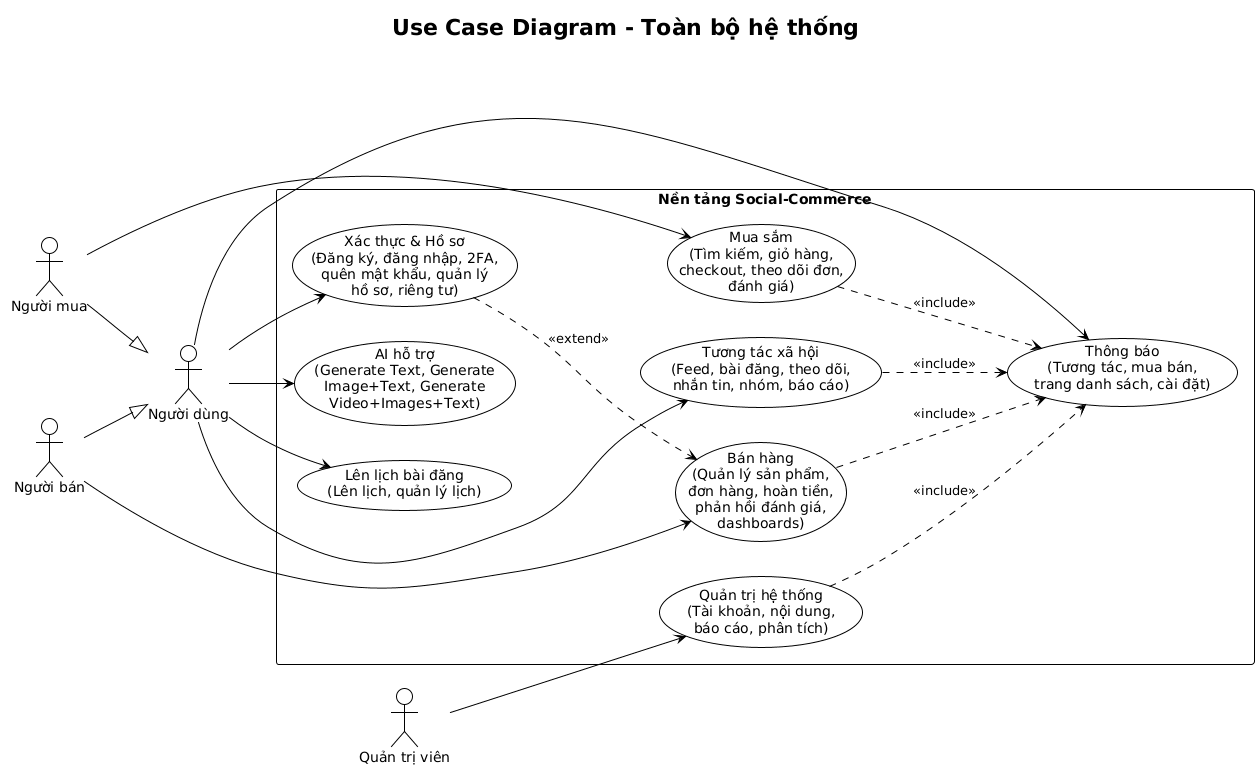
\includegraphics[width=\textwidth]{Images/Usecases/UC-All-System.png}
\caption{Sơ đồ Use Case tổng quan cho toàn hệ thống Social Commerce}
\label{fig:usecase-total}
\end{figure}

\subsection{Module 1: Quản lý Người dùng và Xác thực}
\subsubsection{Module 1: Quản lý Người dùng và Xác thực}
Module này bao gồm các chức năng cốt lõi liên quan đến việc tạo lập, xác thực và quản lý tài khoản người dùng trong hệ thống.

\begin{figure}[H]
\centering
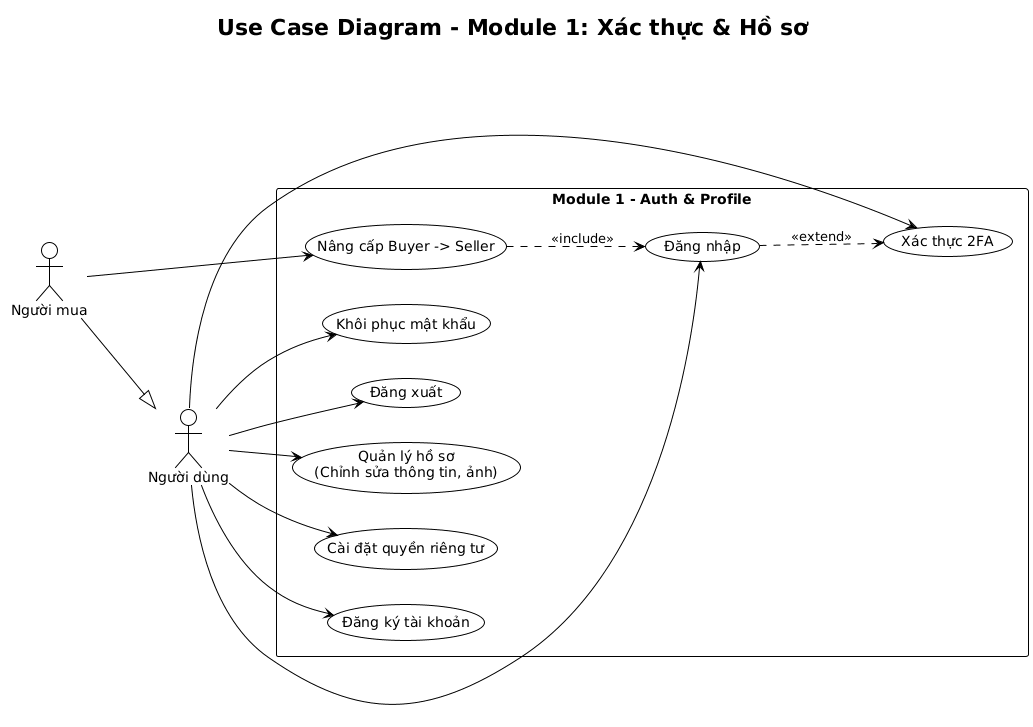
\includegraphics[width=\textwidth]{Images/Usecases/UC-M1-Auth.png}
\caption{Sơ đồ Use Case cho Module 1: Quản lý Người dùng và Xác thực}
\label{fig:usecase-module1}
\end{figure}

% Cấu hình giãn dòng cho bảng dễ đọc hơn
\renewcommand{\arraystretch}{1.3}

% =====================================================
% UC1.1: ĐĂNG KÝ TÀI KHOẢN
% =====================================================
\begin{table}[H]
\centering
\begin{tabularx}{\textwidth}{|l|X|}
\hline
\textbf{Tên Use Case} & \textbf{UC1.1: Đăng ký tài khoản} \\ \hline
\textbf{Tác nhân} & Người dùng chưa đăng nhập \\ \hline
\textbf{Mô tả} & Cho phép người dùng mới tạo một tài khoản trên hệ thống Social Commerce với vai trò mặc định là ``Người mua'' (Buyer). \\ \hline
\textbf{Kích hoạt} & Người dùng nhấn vào nút ``Đăng ký'' trên giao diện. \\ \hline
\textbf{Điều kiện tiên quyết} & 
\begin{itemize}
    \item Người dùng chưa đăng nhập vào hệ thống.
    \item Người dùng có một địa chỉ email hợp lệ và chưa được sử dụng để đăng ký.
\end{itemize} \\ \hline
\textbf{Điều kiện sau} & 
\begin{itemize}
    \item Tài khoản mới được tạo với trạng thái ``chưa xác thực''.
    \item Vai trò người dùng được gán là Buyer.
    \item Hệ thống gửi email/tin nhắn xác thực tài khoản.
    \item Người dùng được chuyển hướng đến trang yêu cầu xác thực.
\end{itemize} \\ \hline
\textbf{Luồng sự kiện chính} & 
\begin{enumerate}
    \item Người dùng truy cập trang Đăng ký.
    \item Người dùng nhập các thông tin bắt buộc.
    \item Người dùng nhấn nút ``Đăng ký''.
    \item Hệ thống kiểm tra tính hợp lệ của dữ liệu.
    \item Hệ thống kiểm tra email đã tồn tại hay chưa.
    \item Hệ thống tạo người dùng mới với trạng thái ``chưa xác thực''.
    \item Hệ thống gửi email/SMS xác thực.
    \item Hệ thống hiển thị thông báo thành công và yêu cầu xác thực.
\end{enumerate} \\ \hline
\textbf{Ngoại lệ} & 
\begin{itemize}
    \item E1: Email không hợp lệ $\rightarrow$ Báo lỗi ``Định dạng email không hợp lệ''.
    \item E2: Mật khẩu xác nhận không khớp $\rightarrow$ Báo lỗi ``Mật khẩu xác nhận không khớp''.
    \item E3: Email đã tồn tại $\rightarrow$ Báo lỗi ``Email này đã được sử dụng''.
    \item E4: Lỗi gửi email $\rightarrow$ Báo lỗi và đề nghị thử lại.
\end{itemize} \\ \hline
\textbf{Ghi chú} & Đây là bước đầu tiên để tham gia vào hệ sinh thái Social Commerce. \\ \hline
\end{tabularx}
\caption{Đặc tả Use Case Đăng ký tài khoản}
\end{table}

% =====================================================
% UC1.2: ĐĂNG NHẬP
% =====================================================
\begin{table}[H]
\centering
\begin{tabularx}{\textwidth}{|l|X|}
\hline
\textbf{Tên Use Case} & \textbf{UC1.2: Đăng nhập vào hệ thống} \\ \hline
\textbf{Tác nhân} & Người dùng chưa đăng nhập \\ \hline
\textbf{Mô tả} & Cho phép người dùng đã có tài khoản truy cập vào hệ thống bằng email và mật khẩu. \\ \hline
\textbf{Kích hoạt} & Người dùng nhấn vào nút ``Đăng nhập'' sau khi điền thông tin. \\ \hline
\textbf{Điều kiện tiên quyết} & Người dùng có một tài khoản đã đăng ký và xác thực. \\ \hline
\textbf{Điều kiện sau} & 
\begin{itemize}
    \item Hệ thống tạo một phiên làm việc (session) cho người dùng.
    \item Hệ thống cấp một JSON Web Token (JWT) để xác thực.
    \item Người dùng được chuyển hướng đến trang chủ.
\end{itemize} \\ \hline
\textbf{Luồng sự kiện chính} & 
\begin{enumerate}
    \item Người dùng truy cập trang Đăng nhập.
    \item Người dùng nhập email và mật khẩu.
    \item Người dùng nhấn nút ``Đăng nhập''.
    \item Hệ thống xác thực thông tin.
    \item Nếu thông tin chính xác và tài khoản không bật 2FA, hệ thống tạo JWT và chuyển hướng người dùng.
\end{enumerate} \\ \hline
\textbf{Ngoại lệ} & 
\begin{itemize}
    \item E1: Sai email hoặc mật khẩu $\rightarrow$ Báo lỗi ``Thông tin đăng nhập không chính xác''.
    \item E2: Tài khoản chưa được xác thực $\rightarrow$ Báo lỗi và yêu cầu xác thực.
    \item E3: Tài khoản bị khóa $\rightarrow$ Báo lỗi ``Tài khoản của bạn đã bị khóa''.
\end{itemize} \\ \hline
\textbf{Ghi chú} & Quá trình xác thực sử dụng JWT để đảm bảo an toàn. \\ \hline
\end{tabularx}
\caption{Đặc tả Use Case Đăng nhập}
\end{table}

% =====================================================
% UC1.3: XÁC THỰC 2 YẾU TỐ (2FA)
% =====================================================
\begin{table}[H]
\centering
\begin{tabularx}{\textwidth}{|l|X|}
\hline
\textbf{Tên Use Case} & \textbf{UC1.3: Sử dụng xác thực hai yếu tố (2FA)} \\ \hline
\textbf{Tác nhân} & Người dùng \\ \hline
\textbf{Mô tả} & Cung cấp một lớp bảo mật bổ sung khi đăng nhập bằng mã xác thực tạm thời. \\ \hline
\textbf{Kích hoạt} & Người dùng có bật 2FA và vừa nhập đúng mật khẩu ở bước đăng nhập. \\ \hline
\textbf{Điều kiện tiên quyết} & 
\begin{itemize}
    \item Người dùng đã kích hoạt tính năng 2FA.
    \item Người dùng đã nhập chính xác email và mật khẩu.
\end{itemize} \\ \hline
\textbf{Điều kiện sau} & 
\begin{itemize}
    \item Danh tính người dùng được xác thực hoàn toàn.
    \item Người dùng được đăng nhập thành công.
\end{itemize} \\ \hline
\textbf{Luồng sự kiện chính} & 
\begin{enumerate}
    \item Hệ thống hiển thị trang nhập mã 2FA.
    \item Người dùng lấy mã từ email (hoặc ứng dụng Authenticator).
    \item Người dùng nhập mã 2FA.
    \item Người dùng nhấn ``Xác nhận''.
    \item Hệ thống kiểm tra mã.
    \item Nếu mã hợp lệ, quá trình đăng nhập hoàn tất.
\end{enumerate} \\ \hline
\textbf{Ngoại lệ} & 
\begin{itemize}
    \item E1: Nhập sai mã 2FA $\rightarrow$ Báo lỗi ``Mã xác thực không chính xác''.
    \item E2: Mã 2FA hết hạn $\rightarrow$ Báo lỗi và yêu cầu thử lại.
\end{itemize} \\ \hline
\textbf{Ghi chú} & Tính năng này tùy chọn và quan trọng cho tài khoản người bán. \\ \hline
\end{tabularx}
\caption{Đặc tả Use Case Xác thực 2FA}
\end{table}

% =====================================================
% UC1.4: KHÔI PHỤC MẬT KHẨU
% =====================================================
\begin{table}[H]
\centering
\begin{tabularx}{\textwidth}{|l|X|}
\hline
\textbf{Tên Use Case} & \textbf{UC1.4: Khôi phục mật khẩu} \\ \hline
\textbf{Tác nhân} & Người dùng chưa đăng nhập \\ \hline
\textbf{Mô tả} & Cho phép người dùng đặt lại mật khẩu trong trường hợp họ quên. \\ \hline
\textbf{Kích hoạt} & Người dùng nhấn vào liên kết ``Quên mật khẩu?'' trên trang Đăng nhập. \\ \hline
\textbf{Điều kiện tiên quyết} & 
\begin{itemize}
    \item Người dùng có một tài khoản đã đăng ký.
    \item Người dùng có quyền truy cập vào email đã đăng ký.
\end{itemize} \\ \hline
\textbf{Điều kiện sau} & Mật khẩu của người dùng được cập nhật thành công. \\ \hline
\textbf{Luồng sự kiện chính} & 
\begin{enumerate}
    \item Người dùng nhấn ``Quên mật khẩu?''.
    \item Hệ thống yêu cầu người dùng nhập email.
    \item Người dùng nhập email và nhấn ``Gửi''.
    \item Hệ thống gửi email chứa liên kết hoặc mã OTP.
    \item Người dùng làm theo hướng dẫn trong email.
    \item Hệ thống chuyển hướng đến trang tạo mật khẩu mới.
    \item Người dùng nhập mật khẩu mới và xác nhận.
    \item Người dùng nhấn ``Lưu thay đổi''.
    \item Hệ thống cập nhật mật khẩu và thông báo thành công.
\end{enumerate} \\ \hline
\textbf{Ngoại lệ} & 
\begin{itemize}
    \item E1: Email không tồn tại $\rightarrow$ Hệ thống hiển thị thông báo chung để bảo mật (tránh lộ danh tính user).
    \item E2: Liên kết/mã OTP hết hạn hoặc không hợp lệ $\rightarrow$ Báo lỗi và yêu cầu làm lại.
    \item E3: Mật khẩu mới không khớp $\rightarrow$ Báo lỗi.
\end{itemize} \\ \hline
\end{tabularx}
\caption{Đặc tả Use Case Khôi phục mật khẩu}
\end{table}

% =====================================================
% UC1.5: ĐĂNG XUẤT
% =====================================================
\begin{table}[H]
\centering
\begin{tabularx}{\textwidth}{|l|X|}
\hline
\textbf{Tên Use Case} & \textbf{UC1.5: Đăng xuất} \\ \hline
\textbf{Tác nhân} & Người dùng \\ \hline
\textbf{Mô tả} & Cho phép người dùng kết thúc phiên làm việc hiện tại một cách an toàn. \\ \hline
\textbf{Kích hoạt} & Người dùng nhấn vào nút ``Đăng xuất''. \\ \hline
\textbf{Điều kiện tiên quyết} & Người dùng đang đăng nhập vào hệ thống. \\ \hline
\textbf{Điều kiện sau} & 
\begin{itemize}
    \item Phiên làm việc của người dùng bị hủy.
    \item JWT trên client bị xóa.
    \item Người dùng được chuyển hướng về trang chủ.
\end{itemize} \\ \hline
\textbf{Luồng sự kiện chính} & 
\begin{enumerate}
    \item Người dùng nhấn nút ``Đăng xuất''.
    \item Hệ thống hủy phiên làm việc và xóa token lưu trữ ở client.
    \item Hệ thống chuyển hướng người dùng về trang chủ.
\end{enumerate} \\ \hline
\end{tabularx}
\caption{Đặc tả Use Case Đăng xuất}
\end{table}

% =====================================================
% UC1.6: QUẢN LÝ HỒ SƠ CÁ NHÂN
% =====================================================
\begin{table}[H]
\centering
\begin{tabularx}{\textwidth}{|l|X|}
\hline
\textbf{Tên Use Case} & \textbf{UC1.6: Quản lý hồ sơ cá nhân} \\ \hline
\textbf{Tác nhân} & Người dùng \\ \hline
\textbf{Mô tả} & Cho phép người dùng xem và chỉnh sửa thông tin cá nhân, ảnh đại diện và ảnh bìa. \\ \hline
\textbf{Kích hoạt} & Người dùng truy cập trang cá nhân và chọn chức năng chỉnh sửa. \\ \hline
\textbf{Điều kiện tiên quyết} & Người dùng đang đăng nhập vào hệ thống. \\ \hline
\textbf{Điều kiện sau} & 
\begin{itemize}
    \item Thông tin cá nhân của người dùng được cập nhật.
    \item Thay đổi được hiển thị ngay lập tức.
\end{itemize} \\ \hline
\textbf{Luồng sự kiện chính} & 
\begin{enumerate}
    \item Người dùng vào trang hồ sơ cá nhân.
    \item Người dùng nhấn ``Chỉnh sửa hồ sơ''.
    \item Người dùng thay đổi thông tin.
    \item Người dùng nhấn ``Lưu thay đổi''.
    \item Hệ thống xác thực và cập nhật dữ liệu.
    \item Hệ thống hiển thị thông báo thành công.
\end{enumerate} \\ \hline
\textbf{Luồng thay thế} & A1: Người dùng nhấn ``Hủy'' $\rightarrow$ Các thay đổi sẽ không được lưu. \\ \hline
\textbf{Ngoại lệ} & 
\begin{itemize}
    \item E1: Lỗi tải lên hình ảnh $\rightarrow$ Báo lỗi tương ứng.
    \item E2: Dữ liệu nhập không hợp lệ $\rightarrow$ Báo lỗi tại trường dữ liệu đó.
\end{itemize} \\ \hline
\textbf{Ghi chú} & Giao diện quản lý cần trực quan và dễ sử dụng. \\ \hline
\end{tabularx}
\caption{Đặc tả Use Case Quản lý hồ sơ}
\end{table}

% =====================================================
% UC1.7: CÀI ĐẶT QUYỀN RIÊNG TƯ
% =====================================================
\begin{table}[H]
\centering
\begin{tabularx}{\textwidth}{|l|X|}
\hline
\textbf{Tên Use Case} & \textbf{UC1.7: Cài đặt quyền riêng tư cho tài khoản} \\ \hline
\textbf{Tác nhân} & Người dùng \\ \hline
\textbf{Mô tả} & Cho phép người dùng tùy chỉnh ai có thể xem hồ sơ, bài đăng hoặc danh sách người theo dõi. \\ \hline
\textbf{Kích hoạt} & Người dùng truy cập vào mục ``Cài đặt \& Quyền riêng tư''. \\ \hline
\textbf{Điều kiện tiên quyết} & Người dùng đang đăng nhập vào hệ thống. \\ \hline
\textbf{Điều kiện sau} & Các thiết lập quyền riêng tư của người dùng được cập nhật. \\ \hline
\textbf{Luồng sự kiện chính} & 
\begin{enumerate}
    \item Người dùng vào trang ``Cài đặt''.
    \item Người dùng chọn tab ``Quyền riêng tư''100.
    \item Người dùng thay đổi các tùy chọn.
    \item Người dùng nhấn ``Lưu thay đổi''.
    \item Hệ thống cập nhật và hiển thị thông báo thành công.
\end{enumerate} \\ \hline
\textbf{Ghi chú} & Tính năng này quan trọng để người dùng cảm thấy an toàn và kiểm soát thông tin. \\ \hline
\end{tabularx}
\caption{Đặc tả Use Case Cài đặt quyền riêng tư}
\end{table}

% =====================================================
% UC1.8: ĐĂNG KÝ NGƯỜI BÁN
% =====================================================
\begin{table}[H]
\centering
\begin{tabularx}{\textwidth}{|l|X|}
\hline
\textbf{Tên Use Case} & \textbf{UC1.8: Đăng ký trở thành Người bán} \\ \hline
\textbf{Tác nhân} & Người dùng (với vai trò Buyer) \\ \hline
\textbf{Mô tả} & Cung cấp quy trình để người dùng ``Người mua'' nâng cấp tài khoản thành ``Người bán''. \\ \hline
\textbf{Kích hoạt} & Người dùng nhấn vào nút ``Trở thành người bán''. \\ \hline
\textbf{Điều kiện tiên quyết} & 
\begin{itemize}
    \item Người dùng đang đăng nhập.
    \item Người dùng hiện có vai trò là Buyer.
\end{itemize} \\ \hline
\textbf{Điều kiện sau} & 
\begin{itemize}
    \item Hồ sơ đăng ký Seller được lưu và chuyển sang trạng thái chờ duyệt (\textit{REVIEWING}) sau khi hoàn thành các bước bắt buộc.
    \item Khi Admin phê duyệt, vai trò người dùng được cập nhật thành Seller.
\end{itemize} \\ \hline
\textbf{Luồng sự kiện chính} & 
\begin{enumerate}
    \item Người dùng truy cập trang ``Đăng ký Bán hàng'' và bắt đầu hồ sơ.
    \item Người dùng hoàn thành bước 1 (thông tin cá nhân/định danh).
    \item Người dùng hoàn thành bước 2 (thông tin kinh doanh).
    \item Người dùng hoàn thành bước 3 (thông tin ngân hàng) và nộp hồ sơ.
    \item Hệ thống chuyển hồ sơ sang trạng thái ``Đang xem xét''.
    \item Admin xét duyệt hồ sơ.
    \item Nếu được duyệt, hệ thống cập nhật vai trò thành Seller và gửi thông báo kết quả.
\end{enumerate} \\ \hline
\textbf{Luồng thay thế} & A1: Người dùng hủy bỏ quá trình đăng ký. \\ \hline
\textbf{Ngoại lệ} & 
\begin{itemize}
    \item E1: Thông tin ở bất kỳ bước nào không hợp lệ $\rightarrow$ Báo lỗi và yêu cầu sửa.
    \item E2: Hồ sơ bị từ chối $\rightarrow$ Hiển thị lý do từ chối để người dùng bổ sung.
\end{itemize} \\ \hline
\textbf{Ghi chú} & Đây là use case cốt lõi thể hiện mô hình ``buyer-to-seller'' của dự án. \\ \hline
\end{tabularx}
\caption{Đặc tả Use Case Đăng ký làm Người bán}
\end{table}

\subsection{Module 2: Tương tác Xã hội}
\subsubsection{Module 2: Tương tác Xã hội}
Module này tập trung vào các tính năng kết nối cộng đồng, chia sẻ nội dung và tương tác giữa người mua và người bán, tạo tiền đề cho các hoạt động thương mại.

\begin{figure}[H]
\centering
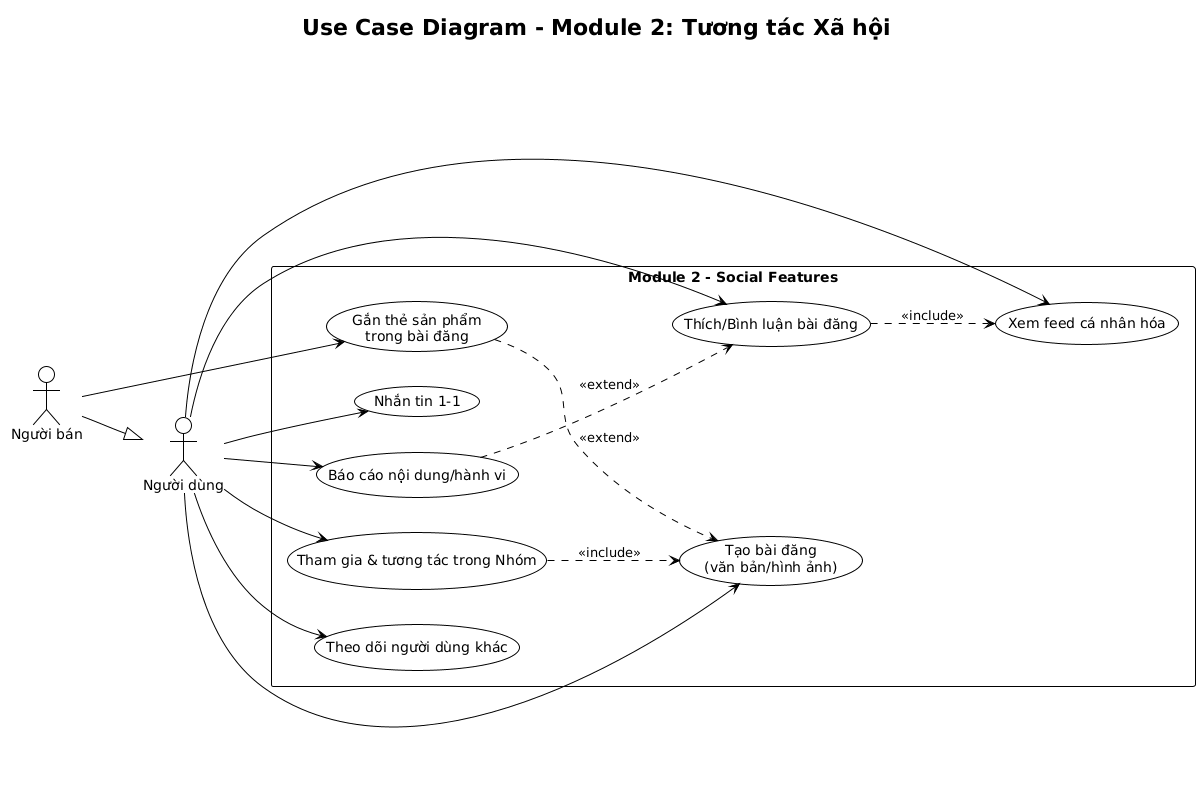
\includegraphics[width=\textwidth]{Images/Usecases/UC-M2-Social.png}
\caption{Sơ đồ Use Case cho Module 2: Tương tác Xã hội}
\label{fig:usecase-module2}
\end{figure}

% Cấu hình giãn dòng
\renewcommand{\arraystretch}{1.3}

% =====================================================
% UC2.1: XEM BẢNG TIN
% =====================================================
\begin{table}[H]
\centering
\begin{tabularx}{\textwidth}{|l|X|}
\hline
\textbf{Tên Use Case} & \textbf{UC2.1: Xem bảng tin (Feed) cá nhân hóa} \\ \hline
\textbf{Tác nhân} & Người dùng \\ \hline
\textbf{Mô tả} & Hiển thị một Bảng tin (Feed) được cá nhân hóa cho người dùng, ưu tiên hiển thị các bài đăng từ những người họ theo dõi và các bài viết có tương tác cao. \\ \hline
\textbf{Kích hoạt} & Người dùng truy cập vào trang chủ sau khi đăng nhập. \\ \hline
\textbf{Điều kiện tiên quyết} & Người dùng đã đăng nhập vào hệ thống. \\ \hline
\textbf{Điều kiện sau} & Người dùng xem được danh sách các bài đăng mới nhất và phù hợp nhất. \\ \hline
\textbf{Luồng sự kiện chính} & 
\begin{enumerate}
    \item Người dùng đăng nhập thành công và được chuyển hướng đến trang chủ.
    \item Hệ thống truy vấn cơ sở dữ liệu để lấy danh sách bài đăng từ những người dùng mà họ đang theo dõi.
    \item Hệ thống cũng lấy các bài đăng có mức độ tương tác cao hoặc được gợi ý.
    \item Hệ thống sắp xếp các bài đăng theo thuật toán (ví dụ: mới nhất, tương tác cao nhất) và hiển thị cho người dùng.
    \item Khi người dùng cuộn trang, hệ thống sẽ tải thêm các bài đăng cũ hơn (infinite scroll).
\end{enumerate} \\ \hline
\textbf{Ngoại lệ} & E1: Lỗi tải dữ liệu $\rightarrow$ Hệ thống hiển thị thông báo lỗi và nút ``Thử lại''. \\ \hline
\textbf{Ghi chú} & Thuật toán sắp xếp feed có thể được cải tiến trong tương lai để tăng tính cá nhân hóa. \\ \hline
\end{tabularx}
\caption{Đặc tả Use Case Xem Bảng tin}
\end{table}

% =====================================================
% UC2.2: TẠO BÀI ĐĂNG
% =====================================================
\begin{table}[H]
\centering
\begin{tabularx}{\textwidth}{|l|X|}
\hline
\textbf{Tên Use Case} & \textbf{UC2.2: Tạo bài đăng (văn bản, hình ảnh)} \\ \hline
\textbf{Tác nhân} & Người dùng \\ \hline
\textbf{Mô tả} & Cho phép người dùng tạo và chia sẻ các bài đăng với nội dung văn bản và hình ảnh lên trang cá nhân của họ và Bảng tin của những người theo dõi. \\ \hline
\textbf{Kích hoạt} & Người dùng nhấn vào nút ``Tạo bài đăng'' trên giao diện. \\ \hline
\textbf{Điều kiện tiên quyết} & Người dùng đã đăng nhập vào hệ thống. \\ \hline
\textbf{Điều kiện sau} & 
\begin{itemize}
    \item Một bài đăng mới được tạo và lưu vào cơ sở dữ liệu.
    \item Bài đăng mới xuất hiện trên trang cá nhân của người dùng và Bảng tin của những người theo dõi.
\end{itemize} \\ \hline
\textbf{Luồng sự kiện chính} & 
\begin{enumerate}
    \item Người dùng nhấn vào ô tạo bài đăng.
    \item Người dùng nhập nội dung văn bản.
    \item Người dùng tùy chọn tải lên một hoặc nhiều hình ảnh.
    \item Người dùng nhấn nút ``Đăng''.
    \item Hệ thống kiểm tra tính hợp lệ của nội dung.
    \item Hệ thống lưu bài đăng vào cơ sở dữ liệu.
    \item Hệ thống hiển thị bài đăng mới ngay trên giao diện của người dùng.
\end{enumerate} \\ \hline
\textbf{Luồng thay thế} & A1: Người dùng hủy bỏ việc tạo bài đăng, nội dung nháp sẽ bị xóa. \\ \hline
\textbf{Ngoại lệ} & 
\begin{itemize}
    \item E1: Lỗi tải lên hình ảnh (kích thước quá lớn, định dạng không hỗ trợ) $\rightarrow$ Hệ thống báo lỗi.
    \item E2: Mất kết nối mạng khi đang đăng bài $\rightarrow$ Hệ thống báo lỗi và lưu lại nội dung nháp (nếu có thể).
\end{itemize} \\ \hline
\end{tabularx}
\caption{Đặc tả Use Case Tạo bài đăng}
\end{table}

% =====================================================
% UC2.3: GẮN THẺ SẢN PHẨM (QUAN TRỌNG)
% =====================================================
\begin{table}[H]
\centering
\begin{tabularx}{\textwidth}{|l|X|}
\hline
\textbf{Tên Use Case} & \textbf{UC2.3: Gắn thẻ sản phẩm vào bài đăng} \\ \hline
\textbf{Tác nhân} & Người bán (Seller) \\ \hline
\textbf{Mô tả} & Cho phép người dùng ``Người bán'' gắn thẻ các sản phẩm từ cửa hàng của mình trực tiếp vào bài đăng, giúp người xem dễ dàng khám phá và mua sản phẩm. \\ \hline
\textbf{Kích hoạt} & Người bán nhấn vào tùy chọn ``Gắn thẻ sản phẩm'' khi đang tạo bài đăng. \\ \hline
\textbf{Điều kiện tiên quyết} & 
\begin{itemize}
    \item Người dùng đã đăng nhập với vai trò Seller.
    \item Người dùng đang trong quá trình tạo hoặc chỉnh sửa một bài đăng.
    \item Người bán đã có ít nhất một sản phẩm trong cửa hàng.
\end{itemize} \\ \hline
\textbf{Điều kiện sau} & Bài đăng được tạo ra có chứa liên kết trực tiếp đến trang sản phẩm đã được gắn thẻ. \\ \hline
\textbf{Luồng sự kiện chính} & 
\begin{enumerate}
    \item Khi đang soạn bài đăng, người bán chọn chức năng ``Gắn thẻ sản phẩm''.
    \item Hệ thống hiển thị danh sách sản phẩm của người bán.
    \item Người bán chọn một sản phẩm để gắn thẻ.
    \item Người bán hoàn tất việc tạo bài đăng và nhấn ``Đăng''.
    \item Hệ thống lưu bài đăng cùng danh sách \texttt{productTags} đã chọn (đa sản phẩm, đa vị trí neo).
    \item Khi hiển thị, bài đăng có thẻ sản phẩm để điều hướng sang trang chi tiết.
\end{enumerate} \\ \hline
\textbf{Ngoại lệ} & E1: Người bán cố gắng gắn thẻ một sản phẩm đã bị xóa hoặc ẩn $\rightarrow$ Hệ thống báo lỗi. \\ \hline
\textbf{Ghi chú} & Đây là tính năng kết nối trực tiếp giữa hoạt động xã hội và thương mại. \\ \hline
\end{tabularx}
\caption{Đặc tả Use Case Gắn thẻ sản phẩm}
\end{table}

% =====================================================
% UC2.4: TƯƠNG TÁC (LIKE/COMMENT)
% =====================================================
\begin{table}[H]
\centering
\begin{tabularx}{\textwidth}{|l|X|}
\hline
\textbf{Tên Use Case} & \textbf{UC2.4: Tương tác với bài đăng} \\ \hline
\textbf{Tác nhân} & Người dùng \\ \hline
\textbf{Mô tả} & Cho phép người dùng thể hiện sự quan tâm hoặc thảo luận về một bài đăng bằng cách nhấn ``Thích'' (Like) hoặc để lại ``Bình luận'' (Comment). \\ \hline
\textbf{Kích hoạt} & Người dùng nhấn vào nút ``Thích'' hoặc ô ``Bình luận'' bên dưới một bài đăng. \\ \hline
\textbf{Điều kiện tiên quyết} & Người dùng đã đăng nhập vào hệ thống. \\ \hline
\textbf{Điều kiện sau} & 
\begin{itemize}
    \item Khi Thích: Lượt thích của bài đăng được tăng lên (hoặc bỏ thích nếu nhấn lại).
    \item Khi Bình luận: Một bình luận mới được thêm vào bài đăng và hiển thị cho người dùng khác.
\end{itemize} \\ \hline
\textbf{Luồng sự kiện chính} & 
\begin{itemize}
    \item \textbf{Thích bài đăng:}
    \begin{enumerate}
        \item Người dùng nhấn vào biểu tượng ``Thích''.
        \item Hệ thống cập nhật số lượt thích và lưu trạng thái ``đã thích'' của người dùng.
    \end{enumerate}
    \item \textbf{Bình luận bài đăng:}
    \begin{enumerate}
        \item Người dùng nhấn vào ô bình luận.
        \item Người dùng nhập nội dung và nhấn gửi.
        \item Hệ thống lưu bình luận và hiển thị nó bên dưới bài đăng.
    \end{enumerate}
\end{itemize} \\ \hline
\textbf{Ngoại lệ} & E1: Mất kết nối mạng $\rightarrow$ Hệ thống báo lỗi, hành động không thực hiện. \\ \hline
\end{tabularx}
\caption{Đặc tả Use Case Tương tác bài đăng}
\end{table}

% =====================================================
% UC2.5: THEO DÕI NGƯỜI DÙNG
% =====================================================
\begin{table}[H]
\centering
\begin{tabularx}{\textwidth}{|l|X|}
\hline
\textbf{Tên Use Case} & \textbf{UC2.5: Theo dõi người dùng khác} \\ \hline
\textbf{Tác nhân} & Người dùng \\ \hline
\textbf{Mô tả} & Cho phép người dùng theo dõi (follow) một người dùng khác để xem các bài đăng của họ trên Bảng tin cá nhân. \\ \hline
\textbf{Kích hoạt} & Người dùng nhấn vào nút ``Theo dõi'' trên trang cá nhân của một người dùng khác. \\ \hline
\textbf{Điều kiện tiên quyết} & Người dùng đã đăng nhập vào hệ thống. \\ \hline
\textbf{Điều kiện sau} & 
\begin{itemize}
    \item Một mối quan hệ ``theo dõi'' được thiết lập.
    \item Các bài đăng trong tương lai của người bị theo dõi sẽ xuất hiện trên Bảng tin của người theo dõi.
\end{itemize} \\ \hline
\textbf{Luồng sự kiện chính} & 
\begin{enumerate}
    \item Người dùng truy cập trang cá nhân của một người khác.
    \item Người dùng nhấn nút ``Theo dõi''.
    \item Hệ thống ghi nhận mối quan hệ theo dõi vào cơ sở dữ liệu.
    \item Nút ``Theo dõi'' chuyển thành ``Đang theo dõi''.
\end{enumerate} \\ \hline
\textbf{Luồng thay thế} & A1: Người dùng nhấn nút ``Hủy theo dõi'' để xóa bỏ mối quan hệ. \\ \hline
\textbf{Ngoại lệ} & E1: Người dùng cố gắng theo dõi chính mình $\rightarrow$ Hệ thống không cho phép. \\ \hline
\end{tabularx}
\caption{Đặc tả Use Case Theo dõi}
\end{table}

% =====================================================
% UC2.6: NHẮN TIN 1-1 (REAL-TIME)
% =====================================================
\begin{table}[H]
\centering
\begin{tabularx}{\textwidth}{|l|X|}
\hline
\textbf{Tên Use Case} & \textbf{UC2.6: Nhắn tin 1-1} \\ \hline
\textbf{Tác nhân} & Người dùng \\ \hline
\textbf{Mô tả} & Cung cấp hệ thống chat thời gian thực cho phép người dùng nhắn tin trực tiếp với nhau, tạo điều kiện cho người mua và người bán trao đổi về sản phẩm. \\ \hline
\textbf{Kích hoạt} & Người dùng nhấn vào nút ``Nhắn tin'' trên trang cá nhân của người khác. \\ \hline
\textbf{Điều kiện tiên quyết} & Người dùng đã đăng nhập vào hệ thống. \\ \hline
\textbf{Điều kiện sau} & 
\begin{itemize}
    \item Tin nhắn được gửi thành công và hiển thị trong cửa sổ chat của cả hai người dùng trong thời gian thực.
    \item Tin nhắn được lưu lại trong lịch sử trò chuyện.
\end{itemize} \\ \hline
\textbf{Luồng sự kiện chính} & 
\begin{enumerate}
    \item Người dùng A mở cuộc hội thoại với người dùng B (tạo mới nếu chưa có).
    \item Người dùng A nhập tin nhắn và nhấn gửi.
    \item Hệ thống lưu tin nhắn vào cơ sở dữ liệu.
    \item Hệ thống phát sự kiện Socket.io theo room hội thoại để cập nhật real-time cho các client đang tham gia.
    \item Nếu người nhận đang offline, hệ thống tạo thông báo để hiển thị khi người nhận quay lại.
\end{enumerate} \\ \hline
\textbf{Ngoại lệ} & 
\begin{itemize}
    \item E1: Người gửi không thuộc cuộc hội thoại $\rightarrow$ Hệ thống từ chối gửi tin nhắn.
    \item E2: Mất kết nối mạng $\rightarrow$ Hệ thống báo lỗi gửi không thành công và cho phép thử lại.
\end{itemize} \\ \hline
\end{tabularx}
\caption{Đặc tả Use Case Nhắn tin}
\end{table}

% =====================================================
% UC2.7: THAM GIA NHÓM
% =====================================================
\begin{table}[H]
\centering
\begin{tabularx}{\textwidth}{|l|X|}
\hline
\textbf{Tên Use Case} & \textbf{UC2.7: Tham gia và tương tác trong Nhóm} \\ \hline
\textbf{Tác nhân} & Người dùng \\ \hline
\textbf{Mô tả} & Cho phép người dùng tham gia vào các Nhóm (Groups) hoặc cộng đồng để thảo luận về những chủ đề chung mà họ quan tâm. \\ \hline
\textbf{Kích hoạt} & Người dùng tìm kiếm và yêu cầu tham gia một nhóm. \\ \hline
\textbf{Điều kiện tiên quyết} & Người dùng đã đăng nhập vào hệ thống. \\ \hline
\textbf{Điều kiện sau} & 
\begin{itemize}
    \item Người dùng trở thành thành viên của nhóm.
    \item Người dùng có thể xem và tạo bài đăng bên trong nhóm đó.
\end{itemize} \\ \hline
\textbf{Luồng sự kiện chính} & 
\begin{enumerate}
    \item Người dùng tìm kiếm hoặc được gợi ý nhóm.
    \item Nhấn ``Tham gia nhóm''.
    \item Nếu nhóm công khai, người dùng trở thành thành viên ngay. Nếu nhóm riêng tư, yêu cầu được gửi để phê duyệt.
    \item Sau khi trở thành thành viên, người dùng có thể tương tác với các nội dung trong nhóm.
\end{enumerate} \\ \hline
\textbf{Luồng thay thế} & A1: Người dùng rời khỏi một nhóm mà họ đã tham gia. \\ \hline
\textbf{Ngoại lệ} & E1: Người dùng bị cấm khỏi nhóm $\rightarrow$ Hệ thống không cho phép tham gia lại. \\ \hline
\end{tabularx}
\caption{Đặc tả Use Case Tham gia Nhóm}
\end{table}

% =====================================================
% UC2.8: BÁO CÁO VI PHẠM
% =====================================================
\begin{table}[H]
\centering
\begin{tabularx}{\textwidth}{|l|X|}
\hline
\textbf{Tên Use Case} & \textbf{UC2.8: Báo cáo nội dung/hành vi vi phạm} \\ \hline
\textbf{Tác nhân} & Người dùng \\ \hline
\textbf{Mô tả} & Cung cấp công cụ để người dùng báo cáo (report) các bài đăng, sản phẩm, hoặc hành vi của người dùng khác mà họ cho là vi phạm. \\ \hline
\textbf{Kích hoạt} & Người dùng nhấn vào tùy chọn ``Báo cáo'' trên một bài đăng, bình luận hoặc trang cá nhân. \\ \hline
\textbf{Điều kiện tiên quyết} & Người dùng đã đăng nhập vào hệ thống. \\ \hline
\textbf{Điều kiện sau} & Một báo cáo được tạo và gửi đến hệ thống quản trị để xem xét. \\ \hline
\textbf{Luồng sự kiện chính} & 
\begin{enumerate}
    \item Người dùng chọn đối tượng cần báo cáo.
    \item Người dùng nhấn vào tùy chọn ``Báo cáo''.
    \item Hệ thống hiển thị biểu mẫu yêu cầu chọn lý do báo cáo.
    \item Người dùng chọn lý do và có thể thêm mô tả chi tiết.
    \item Người dùng nhấn ``Gửi báo cáo''.
    \item Hệ thống ghi nhận báo cáo và thông báo cho người dùng.
\end{enumerate} \\ \hline
\textbf{Ngoại lệ} & E1: Người dùng cố gắng báo cáo cùng một đối tượng nhiều lần trong thời gian ngắn $\rightarrow$ Hệ thống hạn chế để tránh spam. \\ \hline
\textbf{Ghi chú} & Tính năng này giúp duy trì môi trường an toàn và trong sạch cho cộng đồng. \\ \hline
\end{tabularx}
\caption{Đặc tả Use Case Báo cáo vi phạm}
\end{table}

\subsection{Module 3: Hoạt động Thương mại}
\subsubsection{Module 3: Hoạt động Thương mại}
Đây là phân hệ lõi (Core Domain) của hệ thống Social Commerce, nơi diễn ra các hoạt động trao đổi, mua bán hàng hóa giữa các người dùng.

\begin{figure}[H]
\centering
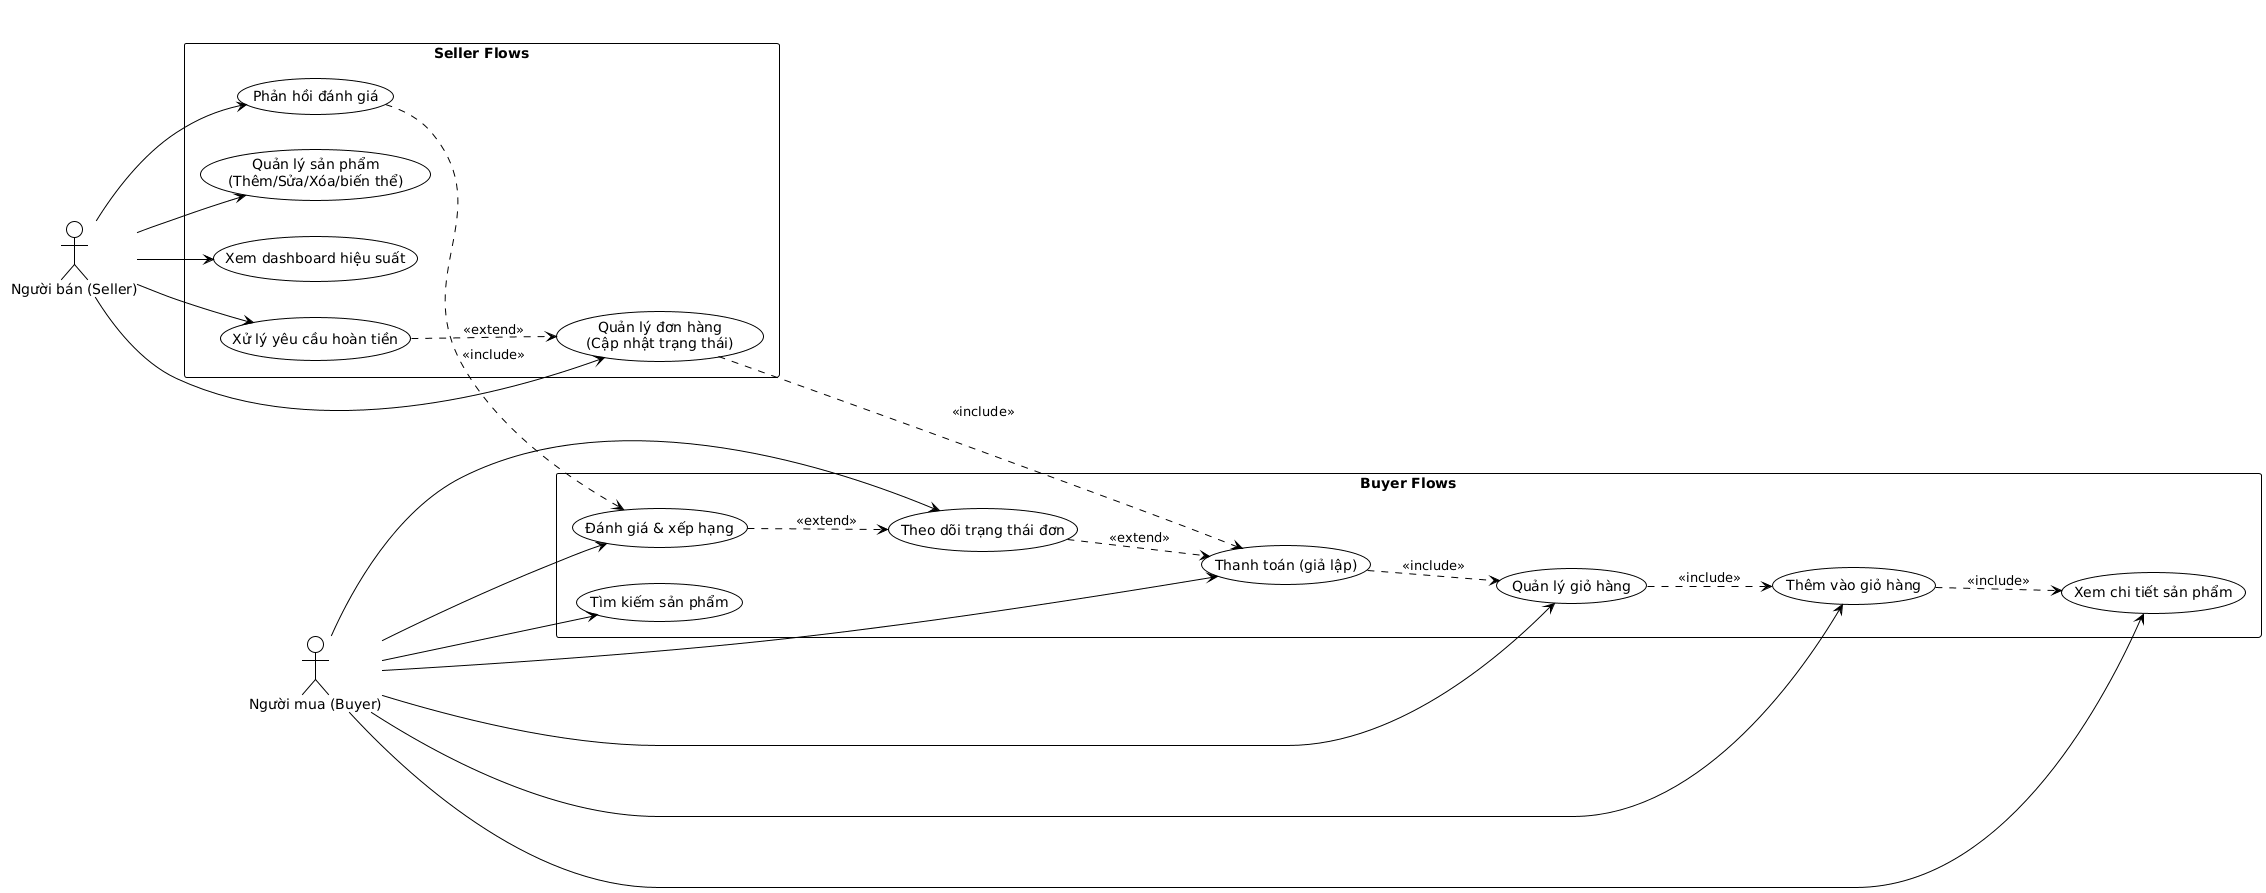
\includegraphics[width=\textwidth]{Images/Usecases/UC-M3-Commerce.png}
\caption{Sơ đồ Use Case cho Module 3: Hoạt động Thương mại}
\label{fig:usecase-module3}
\end{figure}

\renewcommand{\arraystretch}{1.3}

% =====================================================
% PHẦN 1: DÀNH CHO NGƯỜI MUA (BUYER)
% =====================================================
\paragraph{A. Các chức năng dành cho Người mua (Buyer)}

% UC3.1: TÌM KIẾM SẢN PHẨM
\begin{table}[H]
\centering
\begin{tabularx}{\textwidth}{|l|X|}
\hline
\textbf{Tên Use Case} & \textbf{UC3.1: Tìm kiếm sản phẩm} \\ \hline
\textbf{Tác nhân} & Người mua (Buyer) \\ \hline
\textbf{Mô tả} & Cho phép người mua tìm kiếm các sản phẩm họ quan tâm bằng cách sử dụng thanh tìm kiếm và các bộ lọc chi tiết như danh mục và thẻ (tags). \\ \hline
\textbf{Kích hoạt} & Người mua nhập từ khóa vào thanh tìm kiếm hoặc chọn các bộ lọc trên trang sản phẩm. \\ \hline
\textbf{Điều kiện tiên quyết} & Người mua có thể đã đăng nhập hoặc chưa. \\ \hline
\textbf{Điều kiện sau} & Một danh sách các sản phẩm phù hợp với tiêu chí tìm kiếm được hiển thị cho người mua. \\ \hline
\textbf{Luồng sự kiện chính} & 
\begin{enumerate}
    \item Người mua truy cập trang khám phá sản phẩm.
    \item Người mua nhập từ khóa vào thanh tìm kiếm.
    \item Người mua tùy chọn áp dụng các bộ lọc.
    \item Hệ thống truy vấn cơ sở dữ liệu và trả về danh sách sản phẩm khớp.
    \item Giao diện hiển thị kết quả tìm kiếm cho người mua.
\end{enumerate} \\ \hline
\textbf{Ngoại lệ} & E1: Không tìm thấy sản phẩm nào $\rightarrow$ Hệ thống hiển thị thông báo ``Không tìm thấy kết quả phù hợp''. \\ \hline
\end{tabularx}
\caption{Đặc tả Use Case Tìm kiếm sản phẩm}
\end{table}

% UC3.2: XEM CHI TIẾT SẢN PHẨM
\begin{table}[H]
\centering
\begin{tabularx}{\textwidth}{|l|X|}
\hline
\textbf{Tên Use Case} & \textbf{UC3.2: Xem chi tiết sản phẩm} \\ \hline
\textbf{Tác nhân} & Người mua \\ \hline
\textbf{Mô tả} & Cho phép người mua xem thông tin chi tiết về một sản phẩm, bao gồm hình ảnh, mô tả, giá, các biến thể, thông tin người bán và các đánh giá. \\ \hline
\textbf{Kích hoạt} & Người mua nhấp vào một sản phẩm từ kết quả tìm kiếm, Bảng tin hoặc bất kỳ đâu trên nền tảng. \\ \hline
\textbf{Điều kiện tiên quyết} & Sản phẩm phải tồn tại và đang được bán. \\ \hline
\textbf{Điều kiện sau} & Người mua nắm được đầy đủ thông tin về sản phẩm để ra quyết định mua hàng. \\ \hline
\textbf{Luồng sự kiện chính} & 
\begin{enumerate}
    \item Người mua nhấp vào một sản phẩm.
    \item Hệ thống tải và hiển thị trang chi tiết sản phẩm với đầy đủ thông tin.
    \item Người mua có thể xem các hình ảnh, chọn các biến thể (nếu có) và đọc các đánh giá.
\end{enumerate} \\ \hline
\textbf{Ngoại lệ} & E1: Sản phẩm không còn tồn tại hoặc đã bị ẩn $\rightarrow$ Hệ thống hiển thị trang lỗi ``Sản phẩm không tìm thấy''. \\ \hline
\end{tabularx}
\caption{Đặc tả Use Case Xem chi tiết sản phẩm}
\end{table}

% UC3.3: THÊM VÀO GIỎ HÀNG
\begin{table}[H]
\centering
\begin{tabularx}{\textwidth}{|l|X|}
\hline
\textbf{Tên Use Case} & \textbf{UC3.3: Thêm sản phẩm vào giỏ hàng} \\ \hline
\textbf{Tác nhân} & Người mua \\ \hline
\textbf{Mô tả} & Cho phép người mua thêm sản phẩm, bao gồm các biến thể đã chọn, vào giỏ hàng của mình. Người mua có thể thêm sản phẩm từ nhiều cửa hàng khác nhau. \\ \hline
\textbf{Điều kiện tiên quyết} & 
\begin{itemize}
    \item Người mua đã đăng nhập vào hệ thống.
    \item Người mua đã chọn đầy đủ các biến thể bắt buộc của sản phẩm (nếu có).
\end{itemize} \\ \hline
\textbf{Điều kiện sau} & 
\begin{itemize}
    \item Sản phẩm được thêm vào giỏ hàng của người mua.
    \item Biểu tượng giỏ hàng trên giao diện được cập nhật số lượng.
\end{itemize} \\ \hline
\textbf{Luồng sự kiện chính} & 
\begin{enumerate}
    \item Trên trang chi tiết sản phẩm, người mua chọn số lượng và các biến thể mong muốn.
    \item Người mua nhấn ``Thêm vào giỏ hàng''.
    \item Hệ thống xác định biến thể theo \textit{variantId} (hoặc map từ lựa chọn biến thể), kiểm tra trạng thái sản phẩm và tồn kho.
    \item Hệ thống thêm mới hoặc cập nhật cart item tương ứng trong giỏ hàng của người mua.
    \item Hệ thống hiển thị thông báo thành công.
\end{enumerate} \\ \hline
\textbf{Ngoại lệ} & E1: Sản phẩm đã hết hàng $\rightarrow$ Hệ thống báo lỗi và không cho phép thêm vào giỏ. \\ \hline
\end{tabularx}
\caption{Đặc tả Use Case Thêm vào giỏ hàng}
\end{table}

% UC3.4: QUẢN LÝ GIỎ HÀNG
\begin{table}[H]
\centering
\begin{tabularx}{\textwidth}{|l|X|}
\hline
\textbf{Tên Use Case} & \textbf{UC3.4: Quản lý giỏ hàng} \\ \hline
\textbf{Tác nhân} & Người mua \\ \hline
\textbf{Mô tả} & Cho phép người mua xem lại tất cả sản phẩm trong giỏ hàng, cập nhật số lượng, hoặc xóa sản phẩm khỏi giỏ hàng trước khi thanh toán. \\ \hline
\textbf{Kích hoạt} & Người mua nhấp vào biểu tượng giỏ hàng. \\ \hline
\textbf{Điều kiện tiên quyết} & Người mua đã đăng nhập và có ít nhất một sản phẩm trong giỏ hàng. \\ \hline
\textbf{Điều kiện sau} & Giỏ hàng của người mua được cập nhật theo các thay đổi (số lượng, sản phẩm bị xóa). \\ \hline
\textbf{Luồng sự kiện chính} & 
\begin{enumerate}
    \item Người mua truy cập trang giỏ hàng.
    \item Hệ thống hiển thị danh sách các sản phẩm đã thêm.
    \item Người mua có thể: Tăng/giảm số lượng hoặc xóa sản phẩm.
    \item Hệ thống tự động cập nhật lại tổng số tiền.
\end{enumerate} \\ \hline
\textbf{Ngoại lệ} & E1: Cập nhật số lượng vượt quá số lượng tồn kho $\rightarrow$ Hệ thống báo lỗi. \\ \hline
\end{tabularx}
\caption{Đặc tả Use Case Quản lý giỏ hàng}
\end{table}

% UC3.5: THANH TOÁN
\begin{table}[H]
\centering
\begin{tabularx}{\textwidth}{|l|X|}
\hline
\textbf{Tên Use Case} & \textbf{UC3.5: Thực hiện thanh toán} \\ \hline
\textbf{Tác nhân} & Người mua \\ \hline
\textbf{Mô tả} & Cho phép người mua hoàn tất quy trình mua sắm bằng cách cung cấp thông tin giao hàng và thực hiện thanh toán qua một giao diện giả lập. \\ \hline
\textbf{Điều kiện tiên quyết} & 
\begin{itemize}
    \item Người mua đã đăng nhập.
    \item Giỏ hàng có ít nhất một sản phẩm.
\end{itemize} \\ \hline
\textbf{Điều kiện sau} & 
\begin{itemize}
    \item Một đơn hàng mới được tạo trong hệ thống với trạng thái ``PENDING'' và ``paymentStatus=PENDING''.
    \item Giỏ hàng của người mua được làm rỗng.
    \item Người mua được chuyển đến trang xác nhận đơn hàng thành công.
\end{itemize} \\ \hline
\textbf{Luồng sự kiện chính} & 
\begin{enumerate}
    \item Từ giỏ hàng, người mua nhấn ``Thanh toán''.
    \item Hệ thống kiểm tra tồn kho lần cuối cho từng cart item.
    \item Người mua điền thông tin giao hàng.
    \item Người mua chọn phương thức thanh toán (giả lập).
    \item Người mua xác nhận đơn hàng.
    \item Hệ thống tạo bản ghi Order/OrderItem, chốt đơn giá tại thời điểm đặt hàng và trừ tồn kho.
    \item Hệ thống hiển thị thông báo đặt hàng thành công.
\end{enumerate} \\ \hline
\textbf{Ngoại lệ} & E1: Một sản phẩm trong giỏ đã hết hàng $\rightarrow$ Hệ thống báo lỗi và yêu cầu cập nhật giỏ hàng. \\ \hline
\end{tabularx}
\caption{Đặc tả Use Case Thanh toán}
\end{table}

% UC3.6: THEO DÕI ĐƠN HÀNG
\begin{table}[H]
\centering
\begin{tabularx}{\textwidth}{|l|X|}
\hline
\textbf{Tên Use Case} & \textbf{UC3.6: Theo dõi trạng thái đơn hàng} \\ \hline
\textbf{Tác nhân} & Người mua \\ \hline
\textbf{Mô tả} & Cho phép người mua xem danh sách các đơn hàng đã đặt và theo dõi trạng thái hiện tại của chúng (ví dụ: Đang xử lý, Đang giao, Đã giao). \\ \hline
\textbf{Kích hoạt} & Người mua truy cập vào mục ``Đơn hàng của tôi'' trong trang cá nhân. \\ \hline
\textbf{Điều kiện tiên quyết} & Người mua đã đăng nhập và đã đặt ít nhất một đơn hàng. \\ \hline
\textbf{Điều kiện sau} & Người mua biết được tình trạng hiện tại của đơn hàng. \\ \hline
\textbf{Luồng sự kiện chính} & 
\begin{enumerate}
    \item Người mua vào trang quản lý đơn hàng.
    \item Hệ thống hiển thị danh sách tất cả các đơn hàng đã đặt, kèm theo mã đơn hàng, ngày đặt và trạng thái.
    \item Người mua có thể nhấp vào một đơn hàng để xem chi tiết.
\end{enumerate} \\ \hline
\textbf{Ghi chú} & Trạng thái đơn hàng sẽ do Người bán cập nhật (tham chiếu UC3.10). \\ \hline
\end{tabularx}
\caption{Đặc tả Use Case Theo dõi đơn hàng}
\end{table}

% UC3.7: ĐÁNH GIÁ SẢN PHẨM
\begin{table}[H]
\centering
\begin{tabularx}{\textwidth}{|l|X|}
\hline
\textbf{Tên Use Case} & \textbf{UC3.7: Đánh giá và xếp hạng} \\ \hline
\textbf{Tác nhân} & Người mua \\ \hline
\textbf{Mô tả} & Sau khi mua hàng, người mua có thể để lại phản hồi bằng cách viết đánh giá và cho điểm (xếp hạng sao) cho sản phẩm và người bán. \\ \hline
\textbf{Điều kiện tiên quyết} & 
\begin{itemize}
    \item Người mua đã đăng nhập.
    \item Đơn hàng chứa sản phẩm đó phải ở trạng thái ``Đã giao'' hoặc ``Hoàn thành''.
\end{itemize} \\ \hline
\textbf{Điều kiện sau} & 
\begin{itemize}
    \item Một đánh giá mới được lưu vào cơ sở dữ liệu.
    \item Đánh giá và xếp hạng được hiển thị công khai.
\end{itemize} \\ \hline
\textbf{Luồng sự kiện chính} & 
\begin{enumerate}
    \item Người mua vào mục đơn hàng đã giao hoặc hoàn thành.
    \item Người mua chọn sản phẩm muốn đánh giá và nhấn ``Đánh giá''.
    \item Hệ thống hiển thị form đánh giá (chọn sao, viết bình luận, tải ảnh).
    \item Người mua điền thông tin và nhấn ``Gửi đánh giá''.
    \item Hệ thống xác thực quyền theo \textit{orderItemId} và lưu đánh giá.
\end{enumerate} \\ \hline
\textbf{Ngoại lệ} & E1: Người mua cố gắng đánh giá một sản phẩm họ chưa mua hoặc đã đánh giá trước đó $\rightarrow$ Hệ thống không cho phép. \\ \hline
\textbf{Ghi chú} & Đánh giá là một phần quan trọng để xây dựng lòng tin trong cộng đồng. \\ \hline
\end{tabularx}
\caption{Đặc tả Use Case Đánh giá sản phẩm}
\end{table}

\vspace{1cm}

% =====================================================
% PHẦN 2: DÀNH CHO NGƯỜI BÁN (SELLER)
% =====================================================
\paragraph{B. Các chức năng dành cho Người bán (Seller)}

% UC3.8: QUẢN LÝ SẢN PHẨM
\begin{table}[H]
\centering
\begin{tabularx}{\textwidth}{|l|X|}
\hline
\textbf{Tên Use Case} & \textbf{UC3.8: Quản lý sản phẩm} \\ \hline
\textbf{Tác nhân} & Người bán (Seller) \\ \hline
\textbf{Mô tả} & Cung cấp công cụ để người bán thêm, sửa, xóa sản phẩm và quản lý thông tin nâng cao như biến thể (kích cỡ, màu sắc), danh mục và thẻ. \\ \hline
\textbf{Kích hoạt} & Người bán truy cập vào mục ``Quản lý sản phẩm'' trong Bảng điều khiển của mình. \\ \hline
\textbf{Điều kiện tiên quyết} & Người dùng phải đăng nhập với vai trò Seller. \\ \hline
\textbf{Điều kiện sau} & Danh sách sản phẩm của cửa hàng được cập nhật. \\ \hline
\textbf{Luồng sự kiện chính} & 
\begin{enumerate}
    \item Người bán vào trang quản lý sản phẩm và nhấn ``Thêm sản phẩm mới''.
    \item Người bán điền đầy đủ thông tin: tên, mô tả, giá, tồn kho, hình ảnh...
    \item Người bán tùy chọn thêm các biến thể, danh mục, thẻ.
    \item Người bán nhấn ``Lưu''.
    \item Hệ thống xác thực dữ liệu và tạo một bản ghi sản phẩm mới.
    \item Người bán có thể chọn một sản phẩm có sẵn để ``Sửa'' hoặc ``Xóa''.
\end{enumerate} \\ \hline
\textbf{Ngoại lệ} & E1: Dữ liệu nhập vào không hợp lệ (ví dụ: giá âm) $\rightarrow$ Hệ thống báo lỗi. \\ \hline
\textbf{Ghi chú} & Đây là chức năng cốt lõi cho phép người bán đưa hàng hóa lên nền tảng. \\ \hline
\end{tabularx}
\caption{Đặc tả Use Case Quản lý sản phẩm}
\end{table}

% UC3.9: DASHBOARD
\begin{table}[H]
\centering
\begin{tabularx}{\textwidth}{|l|X|}
\hline
\textbf{Tên Use Case} & \textbf{UC3.9: Xem dashboard hiệu suất} \\ \hline
\textbf{Tác nhân} & Người bán \\ \hline
\textbf{Mô tả} & Cung cấp một Bảng điều khiển (dashboard) trực quan để người bán theo dõi hiệu suất kinh doanh qua các chỉ số như lượt xem, doanh số, số đơn hàng... \\ \hline
\textbf{Kích hoạt} & Người bán truy cập vào trang Dashboard chính sau khi đăng nhập. \\ \hline
\textbf{Điều kiện tiên quyết} & Người dùng phải đăng nhập với vai trò Seller. \\ \hline
\textbf{Điều kiện sau} & Người bán nắm được tình hình kinh doanh tổng quan của mình. \\ \hline
\textbf{Luồng sự kiện chính} & 
\begin{enumerate}
    \item Người bán truy cập trang Dashboard.
    \item Hệ thống tổng hợp dữ liệu trong một khoảng thời gian nhất định.
    \item Hệ thống hiển thị dữ liệu dưới dạng các con số, biểu đồ để dễ theo dõi.
    \item Người bán có thể thay đổi khoảng thời gian xem báo cáo.
\end{enumerate} \\ \hline
\textbf{Ghi chú} & Giúp người bán đưa ra các quyết định kinh doanh tốt hơn. \\ \hline
\end{tabularx}
\caption{Đặc tả Use Case Xem Dashboard}
\end{table}

% UC3.10: QUẢN LÝ ĐƠN HÀNG
\begin{table}[H]
\centering
\begin{tabularx}{\textwidth}{|l|X|}
\hline
\textbf{Tên Use Case} & \textbf{UC3.10: Quản lý đơn hàng} \\ \hline
\textbf{Tác nhân} & Người bán \\ \hline
\textbf{Mô tả} & Cho phép người bán xem danh sách các đơn hàng và cập nhật trạng thái của chúng (ví dụ: từ ``Đang xử lý'' sang ``Đang giao''). \\ \hline
\textbf{Kích hoạt} & Người bán truy cập vào mục ``Quản lý đơn hàng'' trong dashboard. \\ \hline
\textbf{Điều kiện tiên quyết} & 
\begin{itemize}
    \item Người dùng phải đăng nhập với vai trò Seller.
    \item Cửa hàng có ít nhất một đơn hàng.
\end{itemize} \\ \hline
\textbf{Điều kiện sau} & Trạng thái của đơn hàng được cập nhật và người mua sẽ thấy được sự thay đổi này. \\ \hline
\textbf{Luồng sự kiện chính} & 
\begin{enumerate}
    \item Người bán vào trang quản lý đơn hàng.
    \item Hệ thống hiển thị danh sách các đơn hàng mới.
    \item Người bán nhấp vào một đơn hàng để xem chi tiết.
    \item Sau khi chuẩn bị xong, người bán thay đổi trạng thái đơn hàng.
    \item Hệ thống lưu lại trạng thái mới.
\end{enumerate} \\ \hline
\end{tabularx}
\caption{Đặc tả Use Case Quản lý đơn hàng của Shop}
\end{table}

% UC3.11: XỬ LÝ HOÀN TIỀN
\begin{table}[H]
\centering
\begin{tabularx}{\textwidth}{|l|X|}
\hline
\textbf{Tên Use Case} & \textbf{UC3.11: Xử lý yêu cầu hoàn tiền} \\ \hline
\textbf{Tác nhân} & Người bán \\ \hline
\textbf{Mô tả} & Cung cấp một quy trình (giả lập) để người bán xem xét và xử lý các yêu cầu hoàn tiền từ người mua. \\ \hline
\textbf{Kích hoạt} & Một người mua gửi yêu cầu hoàn tiền cho một đơn hàng. \\ \hline
\textbf{Điều kiện tiên quyết} & Người dùng phải đăng nhập với vai trò Seller. \\ \hline
\textbf{Điều kiện sau} & Yêu cầu hoàn tiền được giải quyết (chấp nhận hoặc từ chối). \\ \hline
\textbf{Luồng sự kiện chính} & 
\begin{enumerate}
    \item Người bán nhận được thông báo về một yêu cầu hoàn tiền mới.
    \item Người bán vào mục ``Yêu cầu hoàn tiền'' để xem danh sách yêu cầu có trạng thái chờ xử lý.
    \item Người bán đưa ra quyết định ``Chấp nhận'' hoặc ``Từ chối'' yêu cầu.
    \item Nếu chấp nhận, hệ thống cập nhật đơn hàng sang ``REFUNDED''; nếu từ chối, hệ thống lưu lý do từ chối.
    \item Hệ thống ghi nhận quyết định và thông báo lại cho người mua.
    \item Người bán có thể liên hệ với người mua qua tin nhắn để thảo luận thêm.
\end{enumerate} \\ \hline
\textbf{Ghi chú} & Quy trình này được giả lập trong phạm vi đồ án. \\ \hline
\end{tabularx}
\caption{Đặc tả Use Case Xử lý hoàn tiền}
\end{table}

% UC3.12: PHẢN HỒI ĐÁNH GIÁ
\begin{table}[H]
\centering
\begin{tabularx}{\textwidth}{|l|X|}
\hline
\textbf{Tên Use Case} & \textbf{UC3.12: Phản hồi đánh giá} \\ \hline
\textbf{Tác nhân} & Người bán \\ \hline
\textbf{Mô tả} & Cho phép người bán viết phản hồi công khai cho các đánh giá mà người mua đã để lại, giúp tăng cường tương tác và xây dựng niềm tin. \\ \hline
\textbf{Điều kiện tiên quyết} & 
\begin{itemize}
    \item Người dùng phải đăng nhập với vai trò Seller.
    \item Phải có ít nhất một đánh giá từ người mua.
\end{itemize} \\ \hline
\textbf{Điều kiện sau} & Phản hồi của người bán được lưu và hiển thị ngay bên dưới đánh giá của người mua. \\ \hline
\textbf{Luồng sự kiện chính} & 
\begin{enumerate}
    \item Người bán vào mục quản lý đánh giá.
    \item Người bán chọn một đánh giá và nhấn nút ``Phản hồi''.
    \item Người bán nhập nội dung phản hồi và nhấn gửi.
    \item Hệ thống lưu và hiển thị phản hồi đó.
\end{enumerate} \\ \hline
\textbf{Ghi chú} & Đây là một công cụ tốt để thể hiện sự chuyên nghiệp và chăm sóc khách hàng. \\ \hline
\end{tabularx}
\caption{Đặc tả Use Case Phản hồi đánh giá}
\end{table}

\subsection{Module 4: Hệ thống Quản trị}
\subsubsection{Module 4: Hệ thống Quản trị (Admin System)}
Module này cung cấp các công cụ quyền lực cho Quản trị viên (Admin) để giám sát người dùng, kiểm duyệt nội dung và theo dõi sức khỏe của toàn bộ hệ thống.

\begin{figure}[H]
\centering
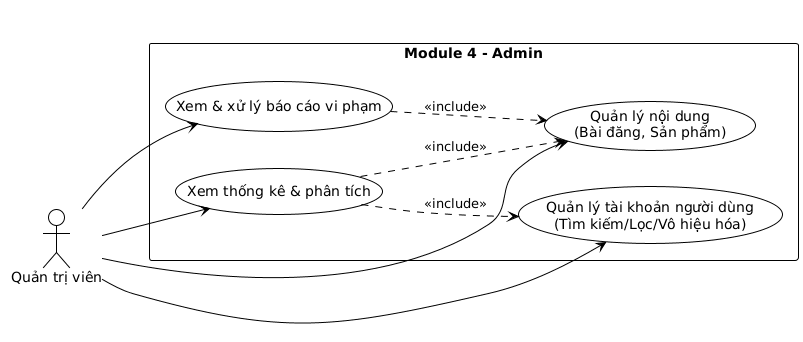
\includegraphics[width=\textwidth]{Images/Usecases/UC-M4-Admin.png}
\caption{Sơ đồ Use Case cho Module 4: Hệ thống Quản trị}
\label{fig:usecase-module4}
\end{figure}

\renewcommand{\arraystretch}{1.3}

% =====================================================
% UC4.1: QUẢN LÝ TÀI KHOẢN NGƯỜI DÙNG
% =====================================================
\begin{table}[H]
\centering
\begin{tabularx}{\textwidth}{|l|X|}
\hline
\textbf{Tên Use Case} & \textbf{UC4.1: Quản lý tài khoản người dùng} \\ \hline
\textbf{Tác nhân} & Quản trị viên (Admin) \\ \hline
\textbf{Mô tả} & Cung cấp cho quản trị viên các công cụ để xem, tìm kiếm, lọc và thực hiện các hành động trên tài khoản người dùng như vô hiệu hóa hoặc cấp lại quyền. \\ \hline
\textbf{Kích hoạt} & Quản trị viên truy cập vào mục ``Quản lý Người dùng'' trong Bảng điều khiển quản trị (Admin Dashboard). \\ \hline
\textbf{Điều kiện tiên quyết} & Quản trị viên đã đăng nhập vào hệ thống với quyền hạn phù hợp. \\ \hline
\textbf{Điều kiện sau} & Thông tin hoặc trạng thái của một hoặc nhiều tài khoản người dùng được thay đổi (ví dụ: tài khoản bị vô hiệu hóa). \\ \hline
\textbf{Luồng sự kiện chính} & 
\begin{enumerate}
    \item Quản trị viên truy cập trang quản lý người dùng.
    \item Hệ thống hiển thị danh sách tất cả người dùng.
    \item Quản trị viên sử dụng các bộ lọc để tìm kiếm người dùng theo tiêu chí.
    \item Quản trị viên chọn một tài khoản người dùng để xem thông tin chi tiết.
    \item Quản trị viên thực hiện một hành động (ví dụ: nhấn nút ``Vô hiệu hóa tài khoản'').
    \item Hệ thống yêu cầu xác nhận hành động.
    \item Quản trị viên xác nhận, và hệ thống cập nhật trạng thái của tài khoản.
\end{enumerate} \\ \hline
\textbf{Ngoại lệ} & 
\begin{itemize}
    \item E1: Quản trị viên cố gắng thực hiện hành động trên tài khoản quản trị viên khác có quyền hạn cao hơn $\rightarrow$ Hệ thống từ chối.
\end{itemize} \\ \hline
\textbf{Ghi chú} & Chức năng này giúp admin duy trì sự kiểm soát đối với cộng đồng người dùng. \\ \hline
\end{tabularx}
\caption{Đặc tả Use Case Quản lý người dùng}
\end{table}

% =====================================================
% UC4.2: QUẢN LÝ NỘI DUNG
% =====================================================
\begin{table}[H]
\centering
\begin{tabularx}{\textwidth}{|l|X|}
\hline
\textbf{Tên Use Case} & \textbf{UC4.2: Quản lý nội dung (Bài đăng/Sản phẩm)} \\ \hline
\textbf{Tác nhân} & Quản trị viên \\ \hline
\textbf{Mô tả} & Cho phép quản trị viên tìm kiếm, xem và xóa các nội dung do người dùng tạo ra như bài đăng hoặc sản phẩm không phù hợp. \\ \hline
\textbf{Kích hoạt} & Quản trị viên truy cập vào các mục quản lý nội dung (ví dụ: ``Quản lý Bài đăng'', ``Quản lý Sản phẩm'') trong dashboard. \\ \hline
\textbf{Điều kiện tiên quyết} & Quản trị viên đã đăng nhập vào hệ thống. \\ \hline
\textbf{Điều kiện sau} & Nội dung không phù hợp (bài đăng, sản phẩm) bị xóa khỏi hệ thống. \\ \hline
\textbf{Luồng sự kiện chính} & 
\begin{enumerate}
    \item Quản trị viên chọn mục nội dung cần quản lý.
    \item Hệ thống hiển thị danh sách các nội dung liên quan.
    \item Quản trị viên sử dụng bộ lọc để tìm kiếm nội dung.
    \item Quản trị viên chọn một nội dung để xem xét.
    \item Nếu nội dung vi phạm, quản trị viên nhấn nút ``Xóa''.
    \item Hệ thống xác nhận và xóa nội dung khỏi cơ sở dữ liệu.
\end{enumerate} \\ \hline
\textbf{Ghi chú} & Việc kiểm duyệt nội dung là cần thiết để giữ cho nền tảng lành mạnh. \\ \hline
\end{tabularx}
\caption{Đặc tả Use Case Quản lý nội dung}
\end{table}

% =====================================================
% UC4.3: XỬ LÝ BÁO CÁO VI PHẠM
% =====================================================
\begin{table}[H]
\centering
\begin{tabularx}{\textwidth}{|l|X|}
\hline
\textbf{Tên Use Case} & \textbf{UC4.3: Xem và xử lý báo cáo vi phạm} \\ \hline
\textbf{Tác nhân} & Quản trị viên \\ \hline
\textbf{Mô tả} & Cho phép quản trị viên xem lại các báo cáo vi phạm được gửi bởi người dùng và đưa ra hành động xử lý phù hợp (ví dụ: xóa nội dung, khóa tài khoản). \\ \hline
\textbf{Điều kiện tiên quyết} & 
\begin{itemize}
    \item Quản trị viên đã đăng nhập vào hệ thống.
    \item Có ít nhất một báo cáo từ người dùng được gửi đến hệ thống.
\end{itemize} \\ \hline
\textbf{Điều kiện sau} & 
\begin{itemize}
    \item Báo cáo được đánh dấu là ``đã xử lý''.
    \item Hành động xử lý đối với nội dung hoặc người dùng bị báo cáo được thực thi.
\end{itemize} \\ \hline
\textbf{Luồng sự kiện chính} & 
\begin{enumerate}
    \item Quản trị viên vào trang quản lý báo cáo.
    \item Hệ thống hiển thị danh sách các báo cáo chưa được xử lý, sắp xếp theo mức độ ưu tiên.
    \item Quản trị viên chọn một báo cáo để xem chi tiết.
    \item Quản trị viên điều hướng đến nội dung/người dùng bị báo cáo để kiểm tra.
    \item Dựa trên kết quả, quản trị viên quyết định hành động (ví dụ: Xóa bài đăng).
    \item Quản trị viên thực hiện hành động thông qua các công cụ quản lý.
    \item Quản trị viên đánh dấu báo cáo là ``Đã xử lý''.
\end{enumerate} \\ \hline
\textbf{Luồng thay thế} & 
\begin{itemize}
    \item A1: Quản trị viên xác định báo cáo là không hợp lệ và đánh dấu là ``Từ chối''.
\end{itemize} \\ \hline
\textbf{Ngoại lệ} & 
\begin{itemize}
    \item E1: Nội dung bị báo cáo đã được người dùng tự xóa trước khi admin xử lý $\rightarrow$ Admin đánh dấu báo cáo là đã giải quyết.
\end{itemize} \\ \hline
\textbf{Ghi chú} & Đây là chức năng tương tác trực tiếp với phản hồi của cộng đồng để duy trì một môi trường an toàn. \\ \hline
\end{tabularx}
\caption{Đặc tả Use Case Xử lý báo cáo}
\end{table}

% =====================================================
% UC4.4: THỐNG KÊ HỆ THỐNG
% =====================================================
\begin{table}[H]
\centering
\begin{tabularx}{\textwidth}{|l|X|}
\hline
\textbf{Tên Use Case} & \textbf{UC4.4: Xem thống kê và phân tích hệ thống} \\ \hline
\textbf{Tác nhân} & Quản trị viên \\ \hline
\textbf{Mô tả} & Cung cấp các biểu đồ và số liệu thống kê trực quan để quản trị viên theo dõi sự phát triển và ``sức khỏe'' của nền tảng. \\ \hline
\textbf{Kích hoạt} & Quản trị viên truy cập vào mục ``Thống kê \& Phân tích'' trong dashboard. \\ \hline
\textbf{Điều kiện tiên quyết} & Quản trị viên đã đăng nhập vào hệ thống. \\ \hline
\textbf{Điều kiện sau} & Quản trị viên nắm được các chỉ số quan trọng về hoạt động của hệ thống để đưa ra quyết định vận hành. \\ \hline
\textbf{Luồng sự kiện chính} & 
\begin{enumerate}
    \item Quản trị viên truy cập trang thống kê.
    \item Hệ thống truy vấn và tổng hợp dữ liệu.
    \item Hệ thống hiển thị các thông tin tổng quan (tổng số người dùng, sản phẩm, bài đăng).
    \item Hệ thống hiển thị các biểu đồ trực quan, chẳng hạn như: Biểu đồ đường thể hiện số lượng người dùng mới; Biểu đồ tròn thể hiện tỷ lệ giữa người mua và người bán.
    \item Quản trị viên có thể thay đổi khoảng thời gian xem thống kê (ví dụ: 7 ngày qua, 30 ngày qua).
\end{enumerate} \\ \hline
\textbf{Ngoại lệ} & 
\begin{itemize}
    \item E1: Lỗi khi tổng hợp dữ liệu $\rightarrow$ Hệ thống báo lỗi.
\end{itemize} \\ \hline
\textbf{Ghi chú} & Các công cụ phân tích này rất quan trọng để theo dõi sự tăng trưởng của hệ thống. \\ \hline
\end{tabularx}
\caption{Đặc tả Use Case Thống kê hệ thống}
\end{table}

\subsection{Module 5: Tích hợp AI Hỗ trợ Sáng tạo Nội dung}
\subsubsection{Module 5: Tích hợp AI Hỗ trợ Sáng tạo}
Đây là tính năng điểm nhấn của dự án, sử dụng Google Gemini API để hỗ trợ người dùng và người bán tạo nội dung đa phương thức chất lượng cao một cách tự động, bao gồm văn bản, hình ảnh và video ngắn. Hệ thống áp dụng pipeline \textbf{Evaluate--Refine Loop}: sau khi gọi API tạo nội dung, kết quả được đánh giá tự động theo các tiêu chí chất lượng (thang điểm 1--10, ngưỡng chấp nhận $\geq$ 7.0). Nếu chưa đạt, hệ thống tự động sửa prompt và thử lại (tối đa 3 lần) trước khi trả kết quả tốt nhất kèm gợi ý chỉnh sửa cho người dùng.

\begin{figure}[H]
\centering
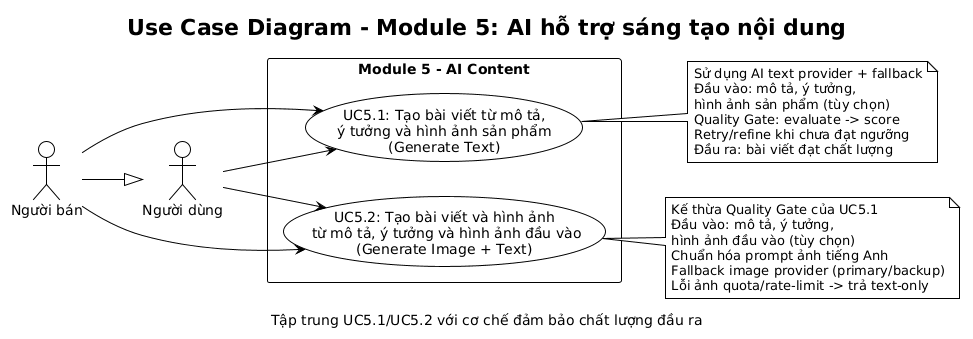
\includegraphics[width=\textwidth]{Images/Usecases/UC-M5-AI.png}
\caption{Sơ đồ Use Case cho Module 5: Tích hợp AI Hỗ trợ Sáng tạo}
\label{fig:usecase-module5}
\end{figure}

\renewcommand{\arraystretch}{1.3}

% UC5.1: GENERATE TEXT
\begin{longtable}{|p{3.5cm}|p{11cm}|}
\caption{Đặc tả Use Case AI Generate Text} \label{tab:uc5.1} \\
\hline
\endfirsthead

\multicolumn{2}{c}%
{{\bfseries \tablename\ \thetable{} -- tiếp tục từ trang trước}} \\
\hline
\endhead

\hline \multicolumn{2}{|r|}{{Tiếp tục ở trang sau}} \\ \hline
\endfoot

\hline
\endlastfoot

\textbf{Tên Use Case} & \textbf{UC5.1: Tạo bài viết từ mô tả, ý tưởng và hình ảnh sản phẩm (Generate Text)} \\ \hline
\textbf{Tác nhân} & Người dùng, Người bán \\ \hline
\textbf{Mô tả} & Cho phép người dùng tạo ra một bài viết hoàn chỉnh dựa trên mô tả, ý tưởng và hình ảnh sản phẩm (nếu có) sử dụng Google Gemini API, với quy trình đánh giá chất lượng tự động và cải thiện prompt khi kết quả chưa đạt. \\ \hline
\textbf{Kích hoạt} & Khi đang soạn thảo bài đăng, người dùng nhấn vào tùy chọn ``Tạo bài viết với AI''. \\ \hline
\textbf{Điều kiện tiên quyết} & 
\begin{itemize}
    \item Người dùng đã đăng nhập và đang trong giao diện tạo bài đăng.
    \item Người dùng đã nhập ít nhất một mô tả hoặc ý tưởng, có thể kèm theo hình ảnh sản phẩm.
\end{itemize} \\ \hline
\textbf{Điều kiện sau} & Một nội dung bài viết hoàn chỉnh (tiêu đề, nội dung, hashtags, CTA) được tạo ra và chèn vào trình soạn thảo, kèm theo điểm đánh giá chất lượng và gợi ý chỉnh sửa (nếu có). \\ \hline
\textbf{Luồng sự kiện chính} & 
\begin{enumerate}
    \item Người dùng nhập mô tả hoặc ý tưởng về bài viết (có thể tải lên hình ảnh sản phẩm).
    \item Người dùng nhấn nút ``Tạo bài viết với AI''.
    \item Hệ thống phân tích đầu vào: trích xuất thực thể chính (tên sản phẩm, đặc điểm, lợi ích), xác định giọng điệu và loại nội dung. Nếu có hình ảnh, phân tích nội dung hình ảnh bằng Gemini Vision.
    \item Hệ thống xây dựng prompt có cấu trúc gồm 5 phần: System Instruction (vai trò chuyên gia nội dung), Context (thông tin thương hiệu, nền tảng), User Input (mô tả + phân tích hình ảnh), Constraints (độ dài 100--300 từ, 5--10 hashtag, phải có CTA), Output Format (JSON schema).
    \item Hệ thống gửi prompt đến Google Gemini API và nhận kết quả.
    \item Hệ thống đánh giá chất lượng kết quả theo 6 tiêu chí có trọng số: Tính liên quan (0.25), Tính hấp dẫn (0.20), Cấu trúc hoàn chỉnh (0.15), Độ dài phù hợp (0.10), Chất lượng ngôn ngữ (0.15), Giá trị thương mại (0.15). Điểm tổng hợp là trung bình có trọng số.
    \item Nếu điểm $\geq$ 7.0/10: hệ thống hiển thị kết quả kèm điểm đánh giá. Nếu điểm $<$ 7.0 và chưa đạt giới hạn 3 lần thử: hệ thống xác định tiêu chí yếu nhất, bổ sung ràng buộc tương ứng vào prompt và gọi lại API (quay lại bước 5). Nếu đã hết lần thử: trả kết quả tốt nhất kèm gợi ý chỉnh sửa.
    \item Hệ thống hiển thị nội dung trong trình soạn thảo kèm điểm đánh giá chi tiết từng tiêu chí và gợi ý cải thiện.
\end{enumerate} \\ \hline
\textbf{Luồng thay thế} & 
\begin{itemize}
    \item A1: Người dùng không hài lòng với kết quả và nhấn ``Tạo lại'' để pipeline chạy lại từ đầu với prompt mới.
    \item A2: Người dùng chỉnh sửa trực tiếp nội dung trong editor (sửa tiêu đề, nội dung, thêm/bớt hashtag).
    \item A3: Người dùng chọn ``Viết lại đoạn này'' để AI viết lại chỉ đoạn được chọn với hướng dẫn cụ thể.
    \item A4: Người dùng thay đổi giọng điệu (chuyên nghiệp, thân thiện, hài hước, sang trọng) và yêu cầu AI viết lại theo giọng điệu mới.
\end{itemize} \\ \hline
\textbf{Ngoại lệ} & 
\begin{itemize}
    \item E1: Lỗi kết nối đến Gemini API $\rightarrow$ Hệ thống báo lỗi ``Không thể tạo nội dung lúc này, vui lòng thử lại sau''.
    \item E2: Hình ảnh không hợp lệ hoặc quá lớn $\rightarrow$ Hệ thống báo lỗi và yêu cầu tải lại hình ảnh.
    \item E3: Gemini API trả về nội dung vi phạm chính sách $\rightarrow$ Hệ thống lọc và yêu cầu tạo lại với prompt đã điều chỉnh.
\end{itemize} \\ \hline
\textbf{Ghi chú} & Pipeline sử dụng chính Gemini API để đánh giá chất lượng (meta-evaluation), kết hợp kiểm tra quy tắc tự động cho các tiêu chí có thể đo lường (format, length, hashtag count). Điểm đánh giá được hiển thị cho người dùng dưới dạng trực quan (thanh tiến trình hoặc biểu đồ radar). \\ \hline
\end{longtable}

% UC5.2: GENERATE IMAGE + TEXT
\begin{longtable}{|p{3.5cm}|p{11cm}|}
\caption{Đặc tả Use Case AI Generate Image + Text} \label{tab:uc5.2} \\
\hline
\endfirsthead

\multicolumn{2}{c}%
{{\bfseries \tablename\ \thetable{} -- tiếp tục từ trang trước}} \\
\hline
\endhead

\hline \multicolumn{2}{|r|}{{Tiếp tục ở trang sau}} \\ \hline
\endfoot

\hline
\endlastfoot

\textbf{Tên Use Case} & \textbf{UC5.2: Tạo bài viết và hình ảnh từ mô tả, ý tưởng và hình ảnh đầu vào (Generate Image + Text)} \\ \hline
\textbf{Tác nhân} & Người dùng, Người bán \\ \hline
\textbf{Mô tả} & Cho phép người dùng tự động tạo ra bài viết kèm hình ảnh dựa trên mô tả, ý tưởng và hình ảnh đầu vào (nếu có) sử dụng Google Gemini API, với đánh giá chất lượng riêng biệt cho text và image. \\ \hline
\textbf{Kích hoạt} & Khi đang soạn thảo bài đăng, người dùng nhấn vào tùy chọn ``Tạo bài viết và hình ảnh với AI''. \\ \hline
\textbf{Điều kiện tiên quyết} & 
\begin{itemize}
    \item Người dùng đã đăng nhập và đang trong giao diện tạo bài đăng.
    \item Người dùng đã nhập ít nhất một mô tả hoặc ý tưởng, có thể kèm theo hình ảnh đầu vào.
\end{itemize} \\ \hline
\textbf{Điều kiện sau} & Một bài viết hoàn chỉnh kèm hình ảnh được tạo bởi AI, cả hai đều được chèn vào trình soạn thảo kèm điểm đánh giá riêng biệt. \\ \hline
\textbf{Luồng sự kiện chính} & 
\begin{enumerate}
    \item Người dùng nhập mô tả hoặc ý tưởng (có thể tải lên hình ảnh đầu vào để tham khảo).
    \item Người dùng nhấn nút ``Tạo bài viết và hình ảnh với AI''.
    \item Hệ thống phân tích đầu vào (tương tự UC5.1), bổ sung phân tích phong cách hình ảnh (màu sắc chủ đạo, bố cục, đối tượng trong ảnh đầu vào).
    \item Hệ thống xây dựng prompt kép: prompt text (5 phần như UC5.1) và prompt image (System Instruction, Context từ text đã tạo, Visual Spec, Constraints về tỷ lệ 1:1/4:5, Negative Prompt).
    \item Hệ thống tạo text trước (với Evaluate--Refine Loop cho text), sau đó sử dụng text đã tạo làm context để tạo image (với Evaluate--Refine Loop riêng cho image).
    \item Đánh giá text: 6 tiêu chí (như UC5.1). Đánh giá image: 4 tiêu chí -- Tính liên quan (0.30), Chất lượng kỹ thuật (0.25), Tính thẩm mỹ (0.25), Nhất quán thương hiệu (0.20). Mỗi loại phải đạt $\geq$ 7.0/10.
    \item Nếu chỉ text hoặc chỉ image chưa đạt: hệ thống chỉ tạo lại phần chưa đạt, giữ nguyên phần đã tốt.
    \item Hệ thống hiển thị bài viết và hình ảnh kèm điểm đánh giá riêng cho từng loại.
\end{enumerate} \\ \hline
\textbf{Luồng thay thế} & 
\begin{itemize}
    \item A1: Người dùng nhấn ``Tạo lại'' để pipeline chạy lại từ đầu.
    \item A2: Người dùng chỉnh sửa text hoặc thay thế hình ảnh riêng biệt.
    \item A3: Người dùng chọn phong cách hình ảnh khác (photorealistic, illustration, flat design) và yêu cầu tạo lại chỉ hình ảnh.
    \item A4: Người dùng tải lên hình ảnh thay thế từ thiết bị, chỉ sử dụng text do AI tạo.
    \item A5: Người dùng yêu cầu AI chỉnh sửa hình ảnh cụ thể (thay đổi màu nền, thêm/bớt đối tượng).
\end{itemize} \\ \hline
\textbf{Ngoại lệ} & 
\begin{itemize}
    \item E1: Lỗi kết nối đến Gemini API $\rightarrow$ Hệ thống báo lỗi ``Không thể tạo nội dung lúc này, vui lòng thử lại sau''.
    \item E2: Gemini API không thể tạo hình ảnh phù hợp sau 3 lần thử $\rightarrow$ Hệ thống trả về bài viết kèm thông báo và gợi ý chỉnh sửa prompt hình ảnh.
    \item E3: Hình ảnh đầu vào không hợp lệ $\rightarrow$ Hệ thống báo lỗi và yêu cầu tải lại hình ảnh.
\end{itemize} \\ \hline
\textbf{Ghi chú} & Hai Evaluate--Refine Loop chạy tuần tự (text trước, image sau) để đảm bảo hình ảnh phù hợp với nội dung text. Chỉ phần chưa đạt ngưỡng mới được tạo lại, tối ưu chi phí gọi API. \\ \hline
\end{longtable}

% UC5.3: GENERATE VIDEO + IMAGES + TEXT
\begin{longtable}{|p{3.5cm}|p{11cm}|}
\caption{Đặc tả Use Case AI Generate Video + Images + Text} \label{tab:uc5.3} \\
\hline
\endfirsthead

\multicolumn{2}{c}%
{{\bfseries \tablename\ \thetable{} -- tiếp tục từ trang trước}} \\
\hline
\endhead

\hline \multicolumn{2}{|r|}{{Tiếp tục ở trang sau}} \\ \hline
\endfoot

\hline
\endlastfoot

\textbf{Tên Use Case} & \textbf{UC5.3: Tạo video ngắn, hình ảnh và bài viết từ mô tả, ý tưởng và hình ảnh đầu vào (Generate Video + Images + Text)} \\ \hline
\textbf{Tác nhân} & Người dùng, Người bán \\ \hline
\textbf{Mô tả} & Tính năng AI nâng cao nhất, tạo bài đăng đa phương thức (video ngắn + tối đa 3 hình ảnh + bài viết) với pipeline đánh giá ba tầng độc lập, sử dụng Google Gemini API và Google Veo 2. \\ \hline
\textbf{Kích hoạt} & Khi đang soạn thảo bài đăng, người dùng nhấn vào tùy chọn ``Tạo video và nội dung đa phương thức với AI''. \\ \hline
\textbf{Điều kiện tiên quyết} & 
\begin{itemize}
    \item Người dùng đã đăng nhập và đang trong giao diện tạo bài đăng.
    \item Người dùng đã nhập ít nhất một mô tả hoặc ý tưởng, có thể kèm theo hình ảnh đầu vào.
\end{itemize} \\ \hline
\textbf{Điều kiện sau} & Một bài đăng đa phương thức hoàn chỉnh (video + images + text) kèm điểm đánh giá từng loại được chèn vào trình soạn thảo. \\ \hline
\textbf{Luồng sự kiện chính} & 
\begin{enumerate}
    \item Người dùng nhập mô tả hoặc ý tưởng (có thể tải lên hình ảnh đầu vào).
    \item Người dùng nhấn nút ``Tạo video và nội dung đa phương thức với AI''.
    \item Hệ thống phân tích đầu vào (tương tự UC5.2), bổ sung xác định storyboard concept (cảnh mở đầu, giới thiệu, highlight, CTA).
    \item Hệ thống thực hiện pipeline tuần tự ba tầng:
    \begin{itemize}
        \item \textbf{Tầng 1 -- Text}: Xây dựng prompt text $\rightarrow$ Gemini API $\rightarrow$ Đánh giá 6 tiêu chí $\rightarrow$ Evaluate--Refine Loop (tối đa 3 lần).
        \item \textbf{Tầng 2 -- Images}: Dùng text làm context $\rightarrow$ Xây dựng prompt image $\rightarrow$ Gemini API tạo tối đa 3 ảnh $\rightarrow$ Đánh giá 4 tiêu chí mỗi ảnh $\rightarrow$ Evaluate--Refine Loop.
        \item \textbf{Tầng 3 -- Video}: Dùng text + images làm context $\rightarrow$ Tự động tạo storyboard $\rightarrow$ Xây dựng prompt video (15--30 giây, tỷ lệ 9:16/1:1) $\rightarrow$ Google Veo 2 $\rightarrow$ Đánh giá 5 tiêu chí: Tính mạch lạc (0.25), Chất lượng hình ảnh (0.25), Độ dài phù hợp (0.15), Tính hấp dẫn (0.20), Nhất quán nội dung (0.15) $\rightarrow$ Evaluate--Refine Loop.
    \end{itemize}
    \item Mỗi tầng Evaluate--Refine Loop chạy độc lập. Khi tạo lại tầng sau, kết quả tầng trước đã đạt được giữ nguyên.
    \item Hệ thống hiển thị video, hình ảnh và bài viết kèm điểm đánh giá chi tiết từng loại. Người dùng có thể chỉnh sửa hoặc tạo lại riêng từng thành phần.
\end{enumerate} \\ \hline
\textbf{Luồng thay thế} & 
\begin{itemize}
    \item A1: Người dùng nhấn ``Tạo lại'' toàn bộ để pipeline chạy lại từ đầu.
    \item A2: Người dùng tạo lại chỉ một thành phần (ví dụ: chỉ video) với yêu cầu bổ sung.
    \item A3: Người dùng chỉnh sửa text, thay thế hình ảnh hoặc video trước khi đăng.
    \item A4: Người dùng cung cấp storyboard chi tiết hơn để cải thiện chất lượng video.
    \item A5: Người dùng chỉ sử dụng một phần nội dung (ví dụ: text + images, bỏ video).
\end{itemize} \\ \hline
\textbf{Ngoại lệ} & 
\begin{itemize}
    \item E1: Lỗi kết nối đến Gemini API hoặc Google Veo 2 $\rightarrow$ Hệ thống báo lỗi.
    \item E2: Gemini API không thể tạo video phù hợp sau 3 lần thử $\rightarrow$ Hệ thống trả về images + text kèm gợi ý cải thiện prompt video.
    \item E3: Hình ảnh đầu vào không hợp lệ $\rightarrow$ Hệ thống báo lỗi.
    \item E4: Video vượt quá 30 giây $\rightarrow$ Kiểm tra rule-based đánh trượt, tự động tạo lại với ràng buộc thời lượng chặt hơn.
\end{itemize} \\ \hline
\textbf{Ghi chú} & Pipeline ba tầng đảm bảo tính nhất quán: text làm nền tảng cho images, text + images làm nền tảng cho video. Đánh giá ``Nhất quán nội dung'' (tiêu chí video) kiểm tra phong cách video có khớp với images và text đã tạo. \\ \hline
\end{longtable}

\subsection{Module 6: Lên lịch và Điều phối Bài đăng}
\subsubsection{Module 6: Lên lịch và Điều phối}
Module này cung cấp tiện ích giúp người dùng và người bán quản lý thời gian đăng bài hiệu quả, đảm bảo nội dung tiếp cận người xem vào khung giờ vàng.

\begin{figure}[H]
\centering
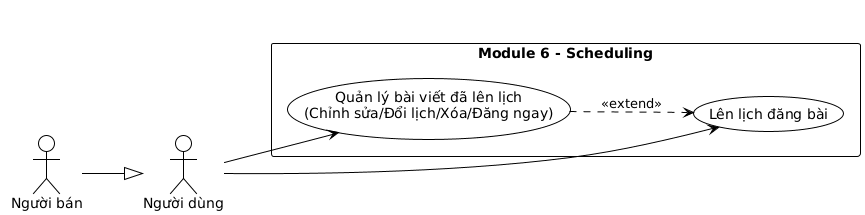
\includegraphics[width=\textwidth]{Images/Usecases/UC-M6-Scheduling.png}
\caption{Sơ đồ Use Case cho Module 6: Lên lịch và Điều phối Bài đăng}
\label{fig:usecase-module6}
\end{figure}

\renewcommand{\arraystretch}{1.3}

% UC6.1: LÊN LỊCH
\begin{table}[H]
\centering
\begin{tabularx}{\textwidth}{|l|X|}
\hline
\textbf{Tên Use Case} & \textbf{UC6.1: Lên lịch đăng bài} \\ \hline
\textbf{Tác nhân} & Người dùng, Người bán \\ \hline
\textbf{Mô tả} & Cung cấp cho người dùng tùy chọn để lên lịch cho một bài đăng, giúp bài viết được tự động xuất bản vào một thời điểm cụ thể trong tương lai. \\ \hline
\textbf{Kích hoạt} & Khi tạo một bài đăng mới, người dùng chọn tùy chọn ``Lên lịch'' thay vì ``Đăng ngay''. \\ \hline
\textbf{Điều kiện tiên quyết} & 
\begin{itemize}
    \item Người dùng đã đăng nhập vào hệ thống.
    \item Người dùng đang ở trong giao diện tạo bài đăng và đã có nội dung cho bài viết.
\end{itemize} \\ \hline
\textbf{Điều kiện sau} & 
\begin{itemize}
    \item Bài đăng được lưu vào cơ sở dữ liệu dưới dạng ``bản nháp đã lên lịch''.
    \item Bài đăng sẽ không hiển thị công khai cho đến đúng thời điểm đã được lên lịch.
\end{itemize} \\ \hline
\textbf{Luồng sự kiện chính} & 
\begin{enumerate}
    \item Trong giao diện tạo bài đăng, sau khi soạn xong nội dung, người dùng chọn tùy chọn ``Lên lịch''.
    \item Một giao diện chọn ngày và giờ trong tương lai sẽ hiện ra.
    \item Người dùng chọn ngày và giờ mong muốn để xuất bản bài viết.
    \item Người dùng nhấn nút ``Xác nhận Lịch''.
    \item Hệ thống lưu bài đăng với trạng thái ``đã lên lịch'' và thời điểm xuất bản đã chọn.
    \item Hệ thống hiển thị thông báo ``Bài viết đã được lên lịch thành công''.
\end{enumerate} \\ \hline
\textbf{Luồng thay thế} & 
\begin{itemize}
    \item A1: Người dùng quyết định không lên lịch nữa và chọn ``Đăng ngay''.
\end{itemize} \\ \hline
\textbf{Ngoại lệ} & 
\begin{itemize}
    \item E1: Người dùng chọn một thời điểm trong quá khứ $\rightarrow$ Hệ thống báo lỗi ``Vui lòng chọn một thời điểm trong tương lai''.
\end{itemize} \\ \hline
\textbf{Ghi chú} & Backend cần có một cơ chế (ví dụ: cron job) để kiểm tra và tự động xuất bản các bài đăng đã đến hạn. \\ \hline
\end{tabularx}
\caption{Đặc tả Use Case Lên lịch đăng bài}
\end{table}

% UC6.2: QUẢN LÝ LỊCH
\begin{table}[H]
\centering
\begin{tabularx}{\textwidth}{|l|X|}
\hline
\textbf{Tên Use Case} & \textbf{UC6.2: Quản lý bài viết đã lên lịch} \\ \hline
\textbf{Tác nhân} & Người dùng, Người bán \\ \hline
\textbf{Mô tả} & Cung cấp một giao diện để người dùng có thể xem lại danh sách các bài viết đang chờ xuất bản, cũng như chỉnh sửa, thay đổi lịch hoặc xóa chúng. \\ \hline
\textbf{Kích hoạt} & Người dùng truy cập vào một mục riêng trong trang cá nhân để xem các bài viết đã lên lịch. \\ \hline
\textbf{Điều kiện tiên quyết} & 
\begin{itemize}
    \item Người dùng đã đăng nhập vào hệ thống.
    \item Người dùng có ít nhất một bài viết đã được lên lịch.
\end{itemize} \\ \hline
\textbf{Điều kiện sau} & Bài viết đã lên lịch được cập nhật (thay đổi nội dung, thời gian) hoặc bị xóa khỏi hàng chờ xuất bản. \\ \hline
\textbf{Luồng sự kiện chính} & 
\begin{enumerate}
    \item Người dùng truy cập vào trang ``Quản lý bài viết đã lên lịch''.
    \item Hệ thống hiển thị danh sách các bài viết đang chờ, kèm theo nội dung xem trước và thời gian dự kiến đăng.
    \item Người dùng chọn một bài viết và thực hiện một trong các hành động: Chỉnh sửa nội dung; Thay đổi lịch; Xóa; Đăng ngay.
    \item Hệ thống cập nhật thay đổi tương ứng vào cơ sở dữ liệu.
\end{enumerate} \\ \hline
\textbf{Luồng thay thế} & 
\begin{itemize}
    \item A1: Người dùng chọn một bài viết và quyết định ``Đăng ngay'' thay vì chờ đến thời gian đã lên lịch.
\end{itemize} \\ \hline
\textbf{Ngoại lệ} & 
\begin{itemize}
    \item E1: Người dùng cố gắng chỉnh sửa một bài viết ngay tại thời điểm nó đang được hệ thống tự động xuất bản $\rightarrow$ Hệ thống báo lỗi hoặc thông báo bài viết đã được đăng.
\end{itemize} \\ \hline
\textbf{Ghi chú} & Giao diện này mang lại sự linh hoạt và quyền kiểm soát hoàn toàn cho người dùng đối với kế hoạch nội dung. \\ \hline
\end{tabularx}
\caption{Đặc tả Use Case Quản lý lịch đăng}
\end{table}

\subsection{Module 7: Hệ thống Thông báo}
\subsubsection{Module 7: Hệ thống Thông báo (Notification)}
Hệ thống thông báo thời gian thực (Real-time) đóng vai trò then chốt trong việc giữ chân người dùng và đảm bảo thông tin mua bán được cập nhật tức thì.

\begin{figure}[H]
\centering
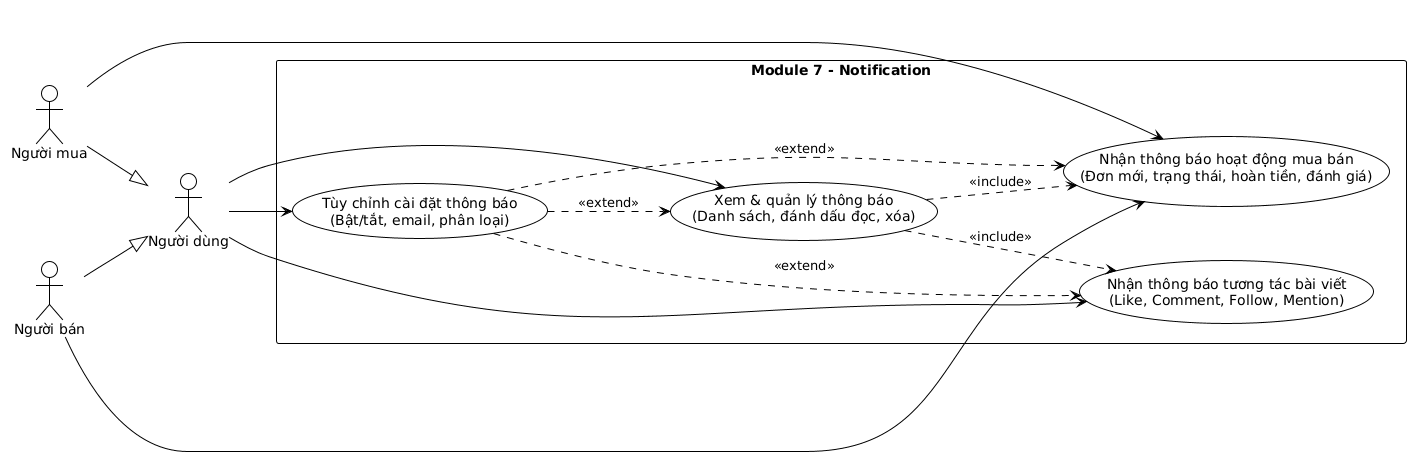
\includegraphics[width=\textwidth]{Images/Usecases/UC-M7-Notification.png}
\caption{Sơ đồ Use Case cho Module 7: Hệ thống Thông báo}
\label{fig:usecase-module7}
\end{figure}

\renewcommand{\arraystretch}{1.3}

% UC7.1: THÔNG BÁO TƯƠNG TÁC
\begin{table}[H]
\centering
\begin{tabularx}{\textwidth}{|l|X|}
\hline
\textbf{Tên Use Case} & \textbf{UC7.1: Nhận thông báo tương tác xã hội} \\ \hline
\textbf{Tác nhân} & Người dùng, Người bán \\ \hline
\textbf{Mô tả} & Hệ thống tự động gửi thông báo ngay lập tức đến người sở hữu bài viết khi có người khác thực hiện các hành động: thích bài viết, bình luận, theo dõi người dùng, hoặc được nhắc đến trong bình luận/bài viết của người khác. \\ \hline
\textbf{Kích hoạt} & Một người dùng khác thực hiện hành động tương tác với bài viết hoặc tài khoản của người nhận. \\ \hline
\textbf{Điều kiện tiên quyết} & 
\begin{itemize}
    \item Người nhận đã đăng nhập vào hệ thống ít nhất một lần trong phiên hiện tại.
    \item Người nhận không tắt hoàn toàn thông báo tương tác xã hội.
\end{itemize} \\ \hline
\textbf{Điều kiện sau} & 
\begin{itemize}
    \item Một thông báo mới xuất hiện trên giao diện người nhận.
    \item Số lượng thông báo chưa đọc tăng lên.
    \item Thông báo được lưu lại để người dùng có thể xem lại sau.
\end{itemize} \\ \hline
\textbf{Luồng sự kiện chính} & 
\begin{enumerate}
    \item Người dùng A thực hiện hành động (ví dụ: thích bài viết của Người dùng B).
    \item Hệ thống phát hiện hành động này.
    \item Hệ thống xác định chủ sở hữu bài viết (Người dùng B).
    \item Hệ thống tạo thông báo mới và gửi ngay lập tức đến Người dùng B.
    \item Giao diện của Người dùng B hiển thị thông báo.
    \item Người dùng B có thể nhấn vào thông báo để chuyển thẳng đến nội dung liên quan.
\end{enumerate} \\ \hline
\textbf{Luồng thay thế} & A1: Người dùng B đang không online $\rightarrow$ Thông báo vẫn được lưu và sẽ hiển thị ngay khi người đó đăng nhập lại. A2: Người dùng B tắt âm thanh thông báo $\rightarrow$ chỉ hiển thị hình ảnh. \\ \hline
\textbf{Ngoại lệ} & 
\begin{itemize}
    \item E1: Người dùng B đã chặn Người dùng A $\rightarrow$ Không gửi thông báo.
    \item E2: Bài viết ở chế độ riêng tư và Người dùng A không được phép xem $\rightarrow$ Không gửi thông báo.
\end{itemize} \\ \hline
\textbf{Ghi chú} & Tính năng quan trọng giúp tăng tính tương tác xã hội. \\ \hline
\end{tabularx}
\caption{Đặc tả Use Case Thông báo tương tác}
\end{table}

% UC7.2: THÔNG BÁO MUA BÁN
\begin{table}[H]
\centering
\begin{tabularx}{\textwidth}{|l|X|}
\hline
\textbf{Tên Use Case} & \textbf{UC7.2: Nhận thông báo hoạt động mua bán} \\ \hline
\textbf{Tác nhân} & Người mua, Người bán \\ \hline
\textbf{Mô tả} & Khi có sự kiện liên quan đến đơn hàng (đặt hàng mới, người bán xác nhận, giao hàng, hoàn thành, hủy đơn, yêu cầu hoàn tiền, có đánh giá mới…), hệ thống gửi thông báo ngay cho cả hai bên liên quan. \\ \hline
\textbf{Kích hoạt} & Bất kỳ thay đổi trạng thái nào của đơn hàng hoặc hành động liên quan đến đơn hàng. \\ \hline
\textbf{Điều kiện tiên quyết} & 
\begin{itemize}
    \item Người nhận có ít nhất một đơn hàng đang trong quá trình xử lý hoặc vừa hoàn tất.
    \item Người nhận chưa tắt thông báo liên quan đến mua bán.
\end{itemize} \\ \hline
\textbf{Điều kiện sau} & 
\begin{itemize}
    \item Cả người mua và người bán đều nhận được thông báo ngay lập tức.
    \item Thông báo chứa liên kết dẫn trực tiếp đến trang chi tiết đơn hàng.
\end{itemize} \\ \hline
\textbf{Luồng sự kiện chính} & 
\begin{enumerate}
    \item Người mua đặt một đơn hàng mới.
    \item Hệ thống tạo thông báo ``Bạn có đơn hàng mới'' gửi đến Người bán.
    \item Người bán xác nhận đơn hàng.
    \item Hệ thống gửi thông báo ``Đơn hàng của bạn đã được xác nhận'' cho Người mua.
    \item Tương tự với các trạng thái: đang giao, đã giao, hoàn thành, hủy, có đánh giá mới, có yêu cầu hoàn tiền…
\end{enumerate} \\ \hline
\textbf{Luồng thay thế} & A1: Một bên đang offline $\rightarrow$ Thông báo được lưu và hiển thị khi đăng nhập lại. A2: Có thể gửi thêm email nếu người dùng bật tùy chọn này. \\ \hline
\textbf{Ngoại lệ} & E1: Đơn hàng bị hủy ngay lập tức bởi người mua trước khi người bán nhìn thấy $\rightarrow$ chỉ gửi thông báo hủy. \\ \hline
\textbf{Ghi chú} & Tính năng này giúp người bán phản hồi nhanh đơn hàng và người mua luôn nắm được trạng thái mua sắm. \\ \hline
\end{tabularx}
\caption{Đặc tả Use Case Thông báo đơn hàng}
\end{table}

% UC7.3: QUẢN LÝ THÔNG BÁO
\begin{table}[H]
\centering
\begin{tabularx}{\textwidth}{|l|X|}
\hline
\textbf{Tên Use Case} & \textbf{UC7.3: Xem và quản lý danh sách thông báo} \\ \hline
\textbf{Tác nhân} & Người dùng \\ \hline
\textbf{Mô tả} & Người dùng có thể mở ra xem toàn bộ danh sách thông báo đã nhận (cả đã đọc và chưa đọc), đánh dấu đã đọc, hoặc xóa thông báo không còn cần thiết. \\ \hline
\textbf{Kích hoạt} & Người dùng nhấn vào biểu tượng chuông hoặc mục ``Thông báo'' trên thanh điều hướng. \\ \hline
\textbf{Điều kiện tiên quyết} & Người dùng đã đăng nhập và từng nhận ít nhất một thông báo. \\ \hline
\textbf{Điều kiện sau} & 
\begin{itemize}
    \item Danh sách thông báo được cập nhật trạng thái đọc/xóa theo hành động của người dùng.
    \item Số lượng thông báo chưa đọc giảm tương ứng.
\end{itemize} \\ \hline
\textbf{Luồng sự kiện chính} & 
\begin{enumerate}
    \item Người dùng nhấn vào biểu tượng thông báo.
    \item Hệ thống hiển thị danh sách tất cả thông báo (mới nhất ở trên).
    \item Thông báo chưa đọc được làm nổi bật.
    \item Người dùng có thể: Nhấn vào thông báo; Đánh dấu đã đọc; Xóa.
    \item Hệ thống cập nhật lại trạng thái và giao diện ngay lập tức.
\end{enumerate} \\ \hline
\textbf{Luồng thay thế} & A1: Người dùng chọn ``Xóa tất cả thông báo'' $\rightarrow$ toàn bộ thông báo bị xóa vĩnh viễn. \\ \hline
\textbf{Ngoại lệ} & E1: Không có thông báo nào $\rightarrow$ hiển thị dòng chữ ``Bạn chưa có thông báo nào''. \\ \hline
\textbf{Ghi chú} & Giao diện nên hỗ trợ phân loại thông báo để dễ theo dõi. \\ \hline
\end{tabularx}
\caption{Đặc tả Use Case Quản lý danh sách thông báo}
\end{table}

% UC7.4: CÀI ĐẶT THÔNG BÁO
\begin{table}[H]
\centering
\begin{tabularx}{\textwidth}{|l|X|}
\hline
\textbf{Tên Use Case} & \textbf{UC7.4: Tùy chỉnh cài đặt thông báo} \\ \hline
\textbf{Tác nhân} & Người dùng \\ \hline
\textbf{Mô tả} & Người dùng có thể tự quyết định sẽ nhận loại thông báo nào, qua kênh nào (trên web, âm thanh, email), và tắt hoàn toàn một số loại thông báo nếu muốn. \\ \hline
\textbf{Kích hoạt} & Người dùng vào phần Cài đặt $\rightarrow$ Thông báo. \\ \hline
\textbf{Điều kiện tiên quyết} & Người dùng đã đăng nhập. \\ \hline
\textbf{Điều kiện sau} & Cài đặt thông báo của người dùng được lưu lại và áp dụng cho mọi phiên đăng nhập sau này. \\ \hline
\textbf{Luồng sự kiện chính} & 
\begin{enumerate}
    \item Người dùng vào Trang cá nhân $\rightarrow$ Cài đặt $\rightarrow$ Thông báo.
    \item Hệ thống hiển thị danh sách các loại thông báo có thể bật/tắt.
    \item Người dùng bật/tắt từng mục và chọn có nhận qua email hay không.
    \item Người dùng nhấn ``Lưu cài đặt''.
    \item Hệ thống lưu và áp dụng ngay lập tức.
\end{enumerate} \\ \hline
\textbf{Luồng thay thế} & A1: Người dùng chọn ``Tắt tất cả thông báo'' $\rightarrow$ toàn bộ thông báo (trừ thông báo hệ thống bắt buộc) sẽ không hiển thị nữa. \\ \hline
\textbf{Ngoại lệ} & Không có. \\ \hline
\textbf{Ghi chú} & Tính năng này quan trọng để tránh làm phiền và tăng trải nghiệm cá nhân hóa. \\ \hline
\end{tabularx}
\caption{Đặc tả Use Case Cài đặt thông báo}
\end{table}

\section{Activity diagram}
Phần này trình bày các Activity Diagrams mô tả dòng chảy nghiệp vụ, điểm quyết định, trạng thái và phản hồi của hệ thống theo từng module. Mỗi module có mô tả tổng quan và các diagram chi tiết với hình ảnh minh họa.

\subsection{Module 1 – Authentication \& Profile}

Module này bao quát hành trình xác thực người dùng: đăng ký, đăng nhập với 2FA, khôi phục mật khẩu, quản lý hồ sơ, cài đặt quyền riêng tư và nâng cấp lên Seller.

\subsubsection{AD-M1-Auth-Register-Login}

Diagram này mô tả quy trình đăng ký và đăng nhập của người dùng, bao gồm ba use case chính.

\textbf{UC1.1 – Đăng ký tài khoản:} Người dùng nhập email, mật khẩu và thông tin cá nhân. Hệ thống kiểm tra tính hợp lệ và email đã tồn tại chưa. Nếu hợp lệ, hệ thống tạo tài khoản với trạng thái \textit{unverified} và gửi email xác thực. Sau khi người dùng xác thực, hệ thống kích hoạt tài khoản.

\textbf{UC1.2 – Đăng nhập:} Người dùng nhập email và mật khẩu. Hệ thống xác thực thông tin. Nếu đúng và không bật 2FA, hệ thống tạo JWT và chuyển hướng đến Trang chủ. Nếu bật 2FA, quy trình chuyển sang UC1.3.

\textbf{UC1.3 – Xác thực hai yếu tố (2FA):} Sau khi xác thực email/mật khẩu, hệ thống gửi mã OTP. Người dùng nhập mã OTP. Nếu mã hợp lệ và chưa hết hạn, hệ thống tạo JWT và chuyển hướng đến Trang chủ.

\begin{figure}[H]
  \centering
  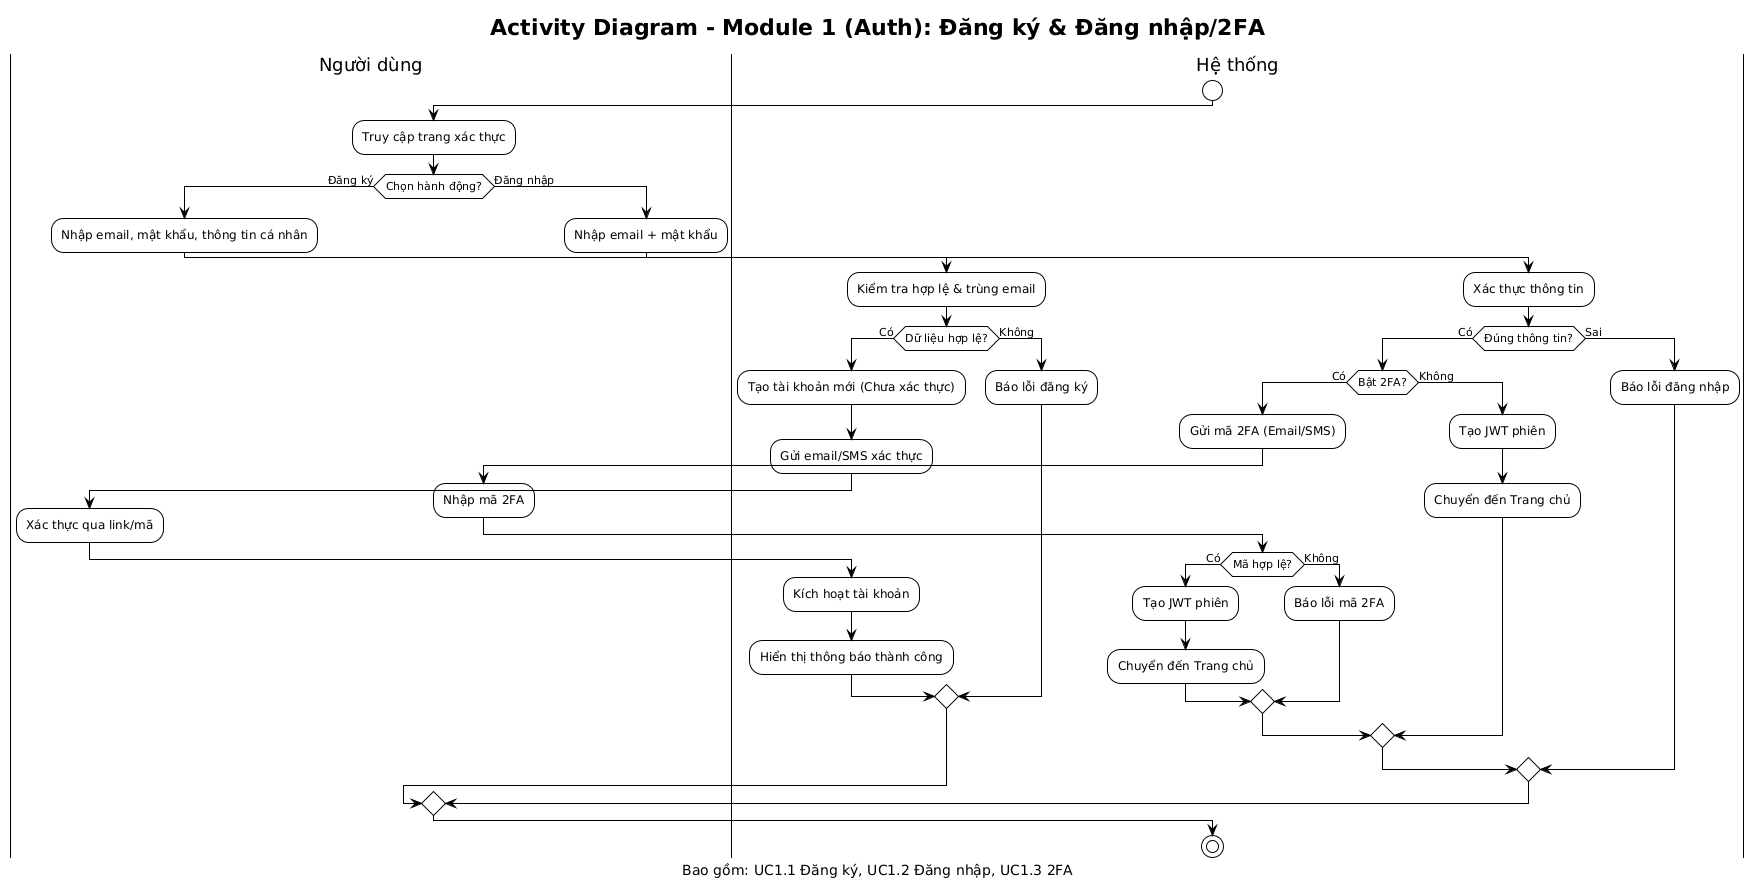
\includegraphics[width=\textwidth]{Images/Activity diagrams/AD-M1-Auth-Register-Login.png}
  \caption{Activity Diagram - Đăng ký và Đăng nhập (AD-M1-Auth-Register-Login)}
\end{figure}

\subsubsection{AD-M1-Auth-Recovery-Logout}

Diagram này mô tả quy trình khôi phục mật khẩu và đăng xuất của người dùng.

\textbf{UC1.4 – Khôi phục mật khẩu:} Người dùng nhập email. Hệ thống kiểm tra và gửi link/mã OTP (bảo mật: luôn trả về thông báo chung). Người dùng mở link/nhập mã và đặt mật khẩu mới. Hệ thống xác thực và cập nhật mật khẩu.

\textbf{UC1.5 – Đăng xuất:} Người dùng nhấn "Đăng xuất". Hệ thống hủy phiên, xóa JWT token và blacklist token trên server, sau đó chuyển hướng về Trang chủ.

\begin{figure}[H]
  \centering
  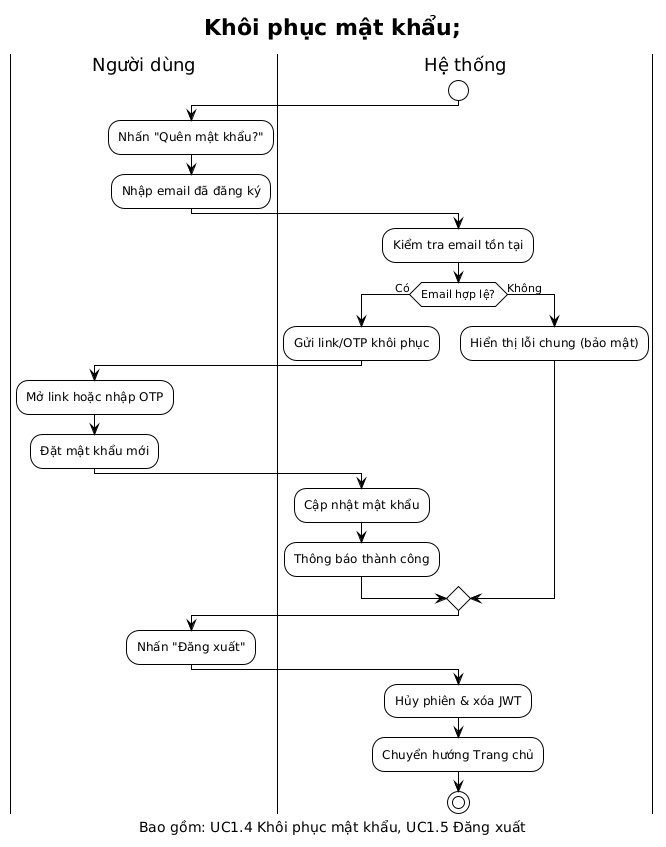
\includegraphics[width=\textwidth]{Images/Activity diagrams/AD-M1-Auth-Recovery-Logout.png}
  \caption{Activity Diagram - Khôi phục mật khẩu và Đăng xuất (AD-M1-Auth-Recovery-Logout)}
\end{figure}

\subsubsection{AD-M1-Profile-EditPrivacy}

Diagram này mô tả quy trình chỉnh sửa hồ sơ cá nhân và cài đặt quyền riêng tư.

\textbf{UC1.6 – Quản lý hồ sơ:} Người dùng cập nhật thông tin (bio, ảnh đại diện, ảnh bìa). Hệ thống upload ảnh (nếu có), xác thực dữ liệu, và cập nhật thông tin trong database. Nếu có lỗi, hệ thống trả về thông báo lỗi cụ thể.

\textbf{UC1.7 – Quyền riêng tư:} Người dùng điều chỉnh cài đặt ai có thể xem hồ sơ, bài đăng và nhắn tin (công khai, chỉ bạn bè, chỉ mình tôi). Hệ thống lưu cấu hình vào database và áp dụng ngay lập tức.

\begin{figure}[H]
  \centering
  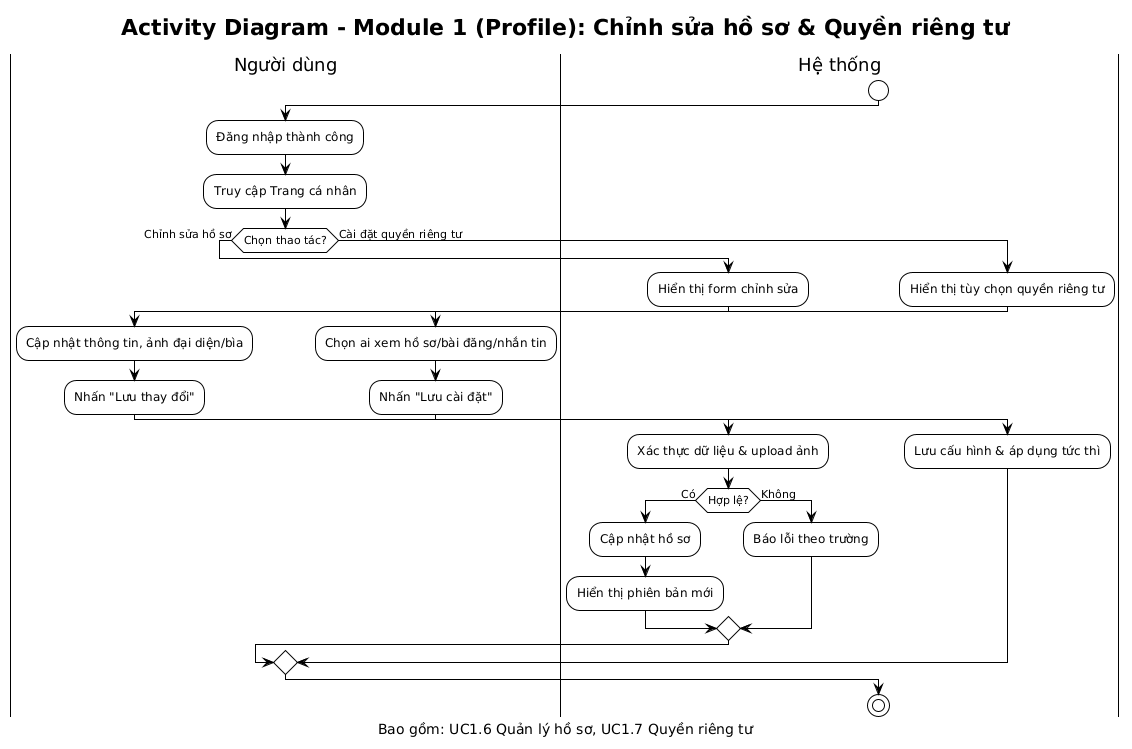
\includegraphics[width=\textwidth]{Images/Activity diagrams/AD-M1-Profile-EditPrivacy.png}
  \caption{Activity Diagram - Chỉnh sửa hồ sơ và Quyền riêng tư (AD-M1-Profile-EditPrivacy)}
\end{figure}

\subsubsection{AD-M1-Profile-SellerUpgrade}

Diagram này mô tả quy trình đăng ký trở thành người bán (Seller).

\textbf{UC1.8 – Đăng ký Người bán:} Buyer điền form đăng ký với thông tin shop (tên shop, địa chỉ, số điện thoại, giấy tờ pháp lý). Hệ thống lưu với trạng thái \textit{pending} và gửi email xác minh. Sau khi xác minh thành công, hệ thống cập nhật trạng thái thành \textit{approved}, thay đổi vai trò từ \textit{buyer} sang \textit{seller}, và chuyển hướng đến Seller Dashboard.

\begin{figure}[H]
  \centering
  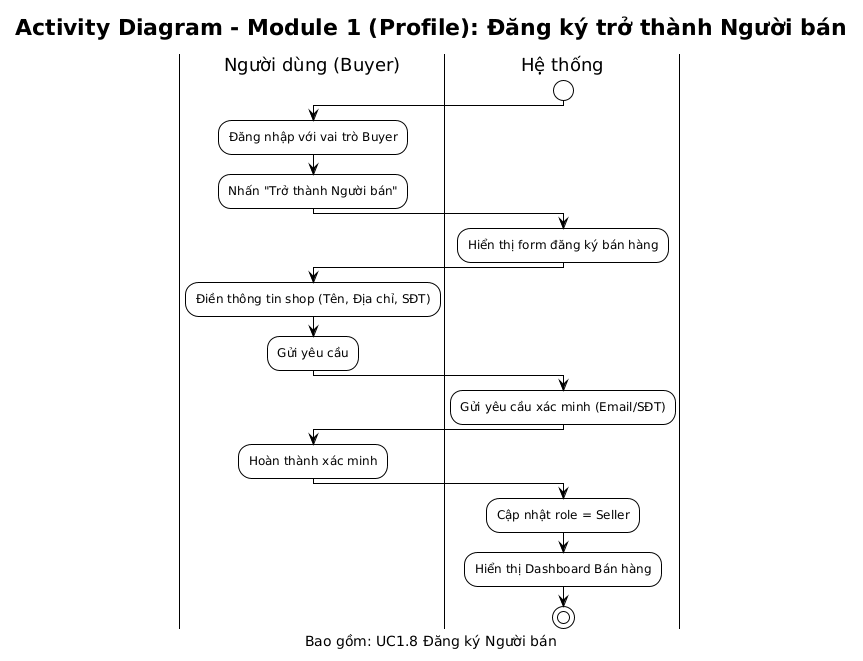
\includegraphics[width=\textwidth]{Images/Activity diagrams/AD-M1-Profile-SellerUpgrade.png}
  \caption{Activity Diagram - Đăng ký trở thành Người bán (AD-M1-Profile-SellerUpgrade)}
\end{figure}

\subsection{Module 2 – Social \& Content}

Module này tập trung vào các tính năng mạng xã hội: xem feed cá nhân hóa, tạo và quản lý bài đăng, tương tác, follow, nhắn tin, tham gia nhóm, và báo cáo vi phạm.

\subsubsection{AD-M2-FeedAndPosts}

Diagram này mô tả quy trình xem feed, tạo bài đăng và tương tác với nội dung.

\textbf{UC2.1 – Xem Feed:} Người dùng truy cập Trang chủ. Hệ thống truy vấn database lấy bài đăng từ người đang theo dõi kết hợp gợi ý, áp dụng thuật toán sắp xếp. Feed hiển thị với tính năng infinite scroll.

\textbf{UC2.2 – Tạo bài đăng:} Người dùng nhập nội dung văn bản và tải hình ảnh (nếu có). Seller có thể gắn thẻ sản phẩm (UC2.3). Hệ thống kiểm tra nội dung, lưu bài đăng vào database, và hiển thị trên feed.

\textbf{UC2.3 – Gắn thẻ sản phẩm:} Seller chọn một hoặc nhiều sản phẩm từ shop để gắn thẻ vào bài đăng. Người dùng xem bài đăng có thể nhấn vào thẻ sản phẩm để chuyển đến trang chi tiết.

\textbf{UC2.4 – Tương tác với bài đăng:} Người dùng có thể thích hoặc bình luận bài đăng. Hệ thống cập nhật số lượt thích/bình luận, lưu vào database và gửi thông báo đến chủ sở hữu bài đăng (UC7.1).

\begin{figure}[H]
  \centering
  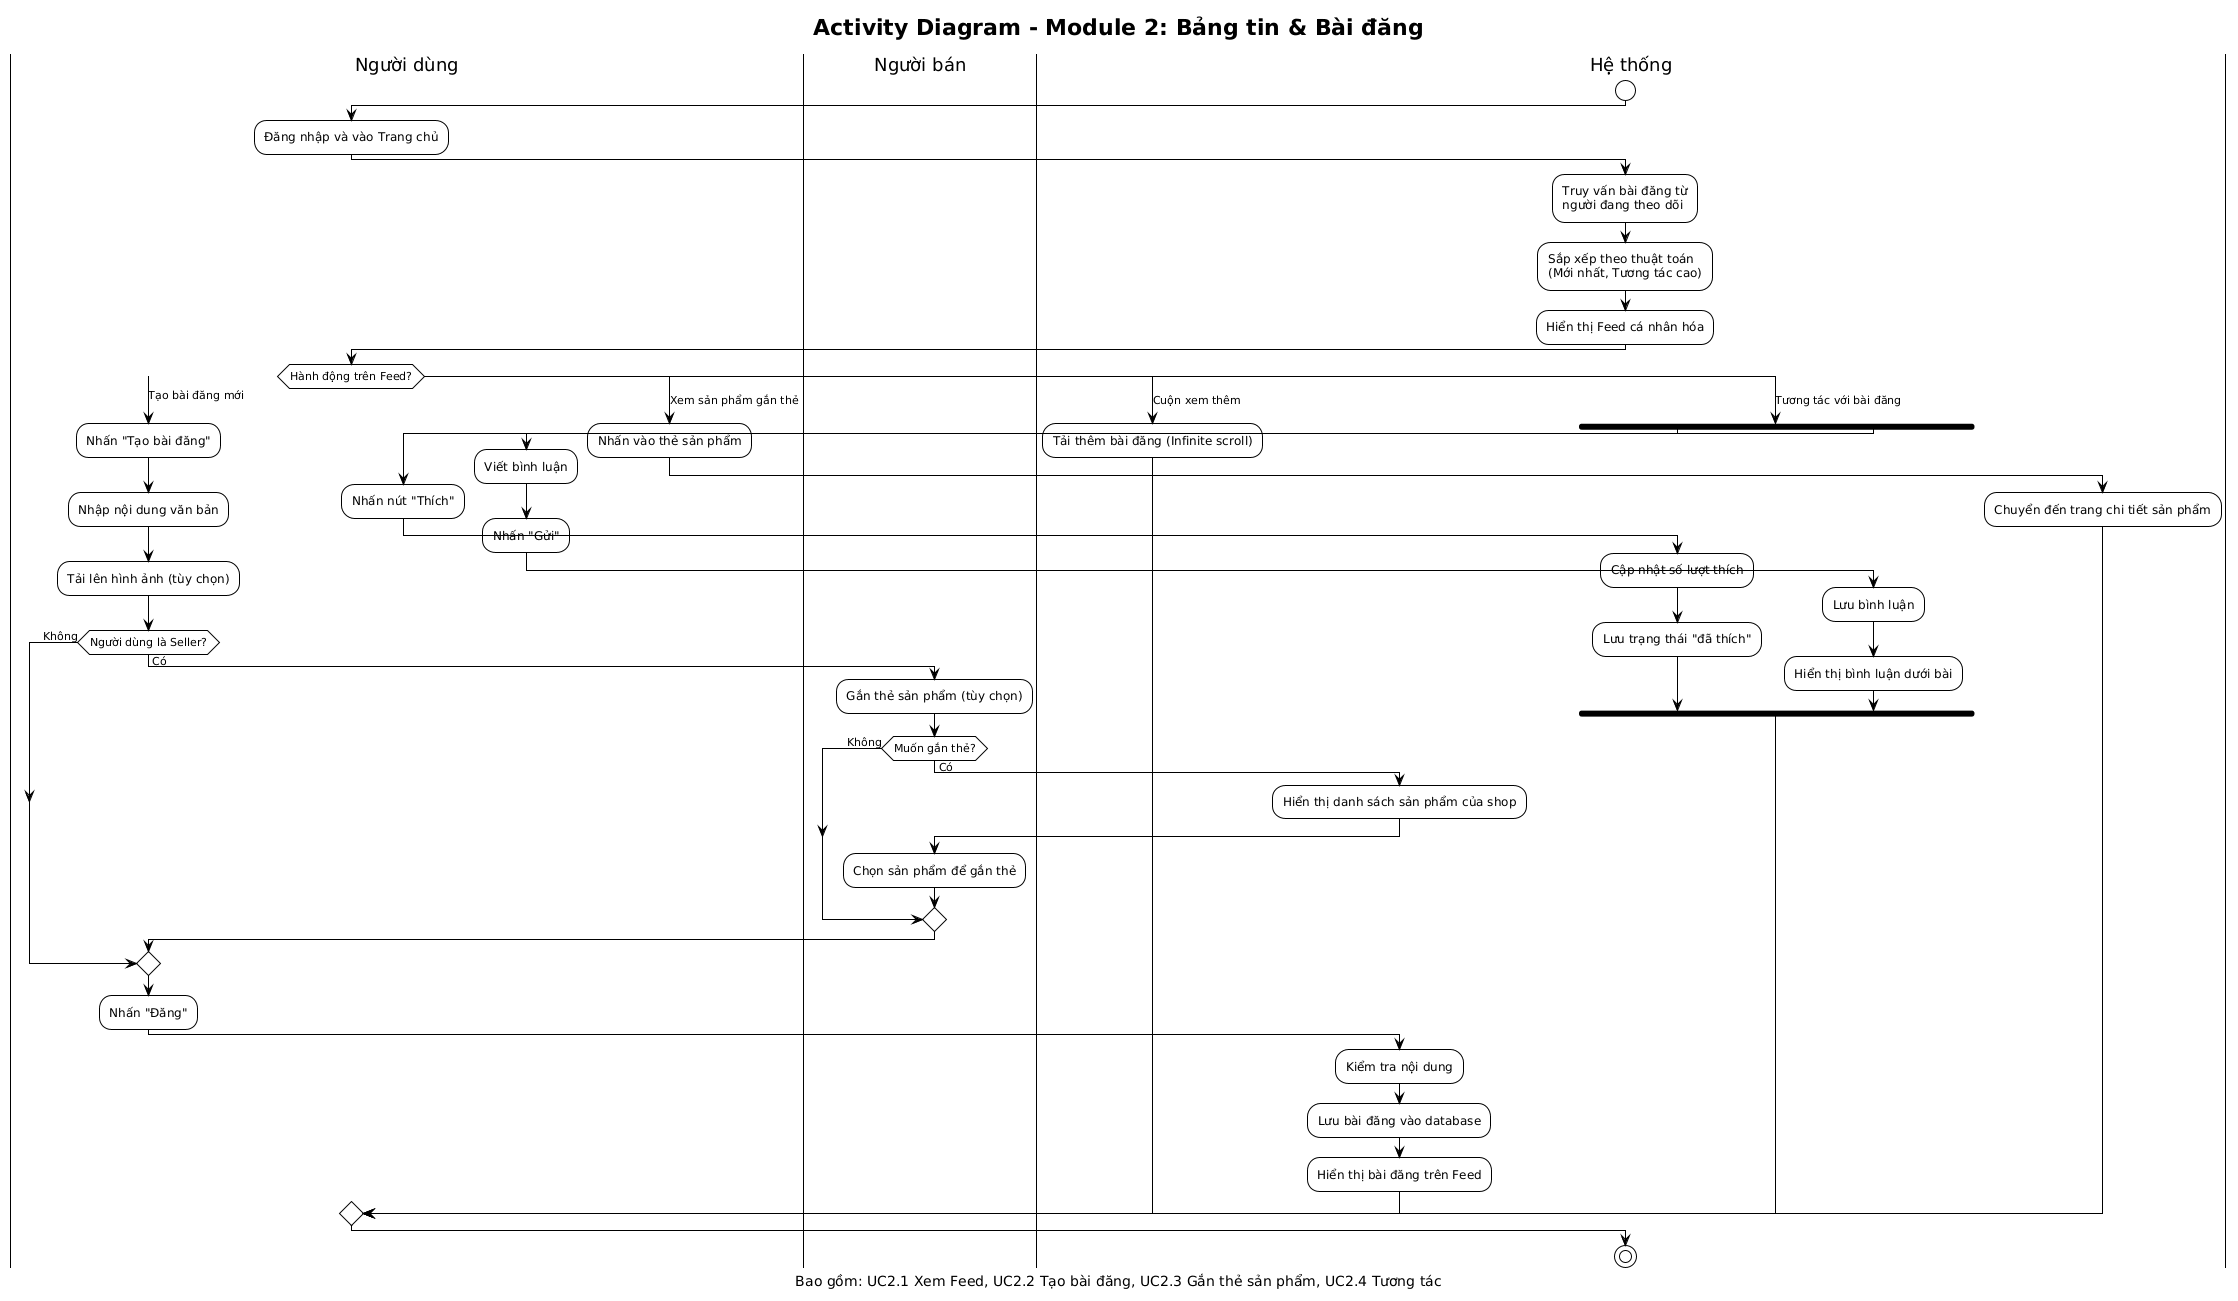
\includegraphics[width=\textwidth]{Images/Activity diagrams/AD-M2-FeedAndPosts.png}
  \caption{Activity Diagram - Feed và Bài đăng (AD-M2-FeedAndPosts)}
\end{figure}

\subsubsection{AD-M2-SocialConnections}

Diagram này mô tả các kết nối xã hội giữa người dùng, bao gồm follow, nhắn tin, tham gia nhóm và báo cáo vi phạm.

\textbf{UC2.5 – Theo dõi người dùng:} Người dùng A nhấn "Theo dõi" trên trang cá nhân của B. Hệ thống tạo mối quan hệ follow, cập nhật số người theo dõi, gửi thông báo đến B, và bài đăng của B sẽ xuất hiện trên Feed của A.

\textbf{UC2.6 – Nhắn tin 1-1:} Người dùng A gửi tin nhắn cho B. Hệ thống kiểm tra B có chặn A hay không. Nếu không bị chặn, hệ thống lưu tin nhắn vào database và gửi real-time đến B qua WebSocket (Socket.io).

\textbf{UC2.7 – Tham gia nhóm:} Người dùng A chọn nhóm và nhấn "Tham gia". Nếu là nhóm công khai, hệ thống thêm A vào nhóm ngay lập tức. Nếu là nhóm riêng tư, hệ thống gửi yêu cầu và chờ Admin phê duyệt.

\textbf{UC2.8 – Báo cáo vi phạm:} Người dùng A chọn đối tượng báo cáo (bài đăng, bình luận hoặc người dùng), chọn lý do vi phạm và thêm mô tả (nếu có). Hệ thống lưu báo cáo với trạng thái \textit{pending}, thông báo Admin và hiển thị "Báo cáo đã được ghi nhận".

\begin{figure}[H]
  \centering
  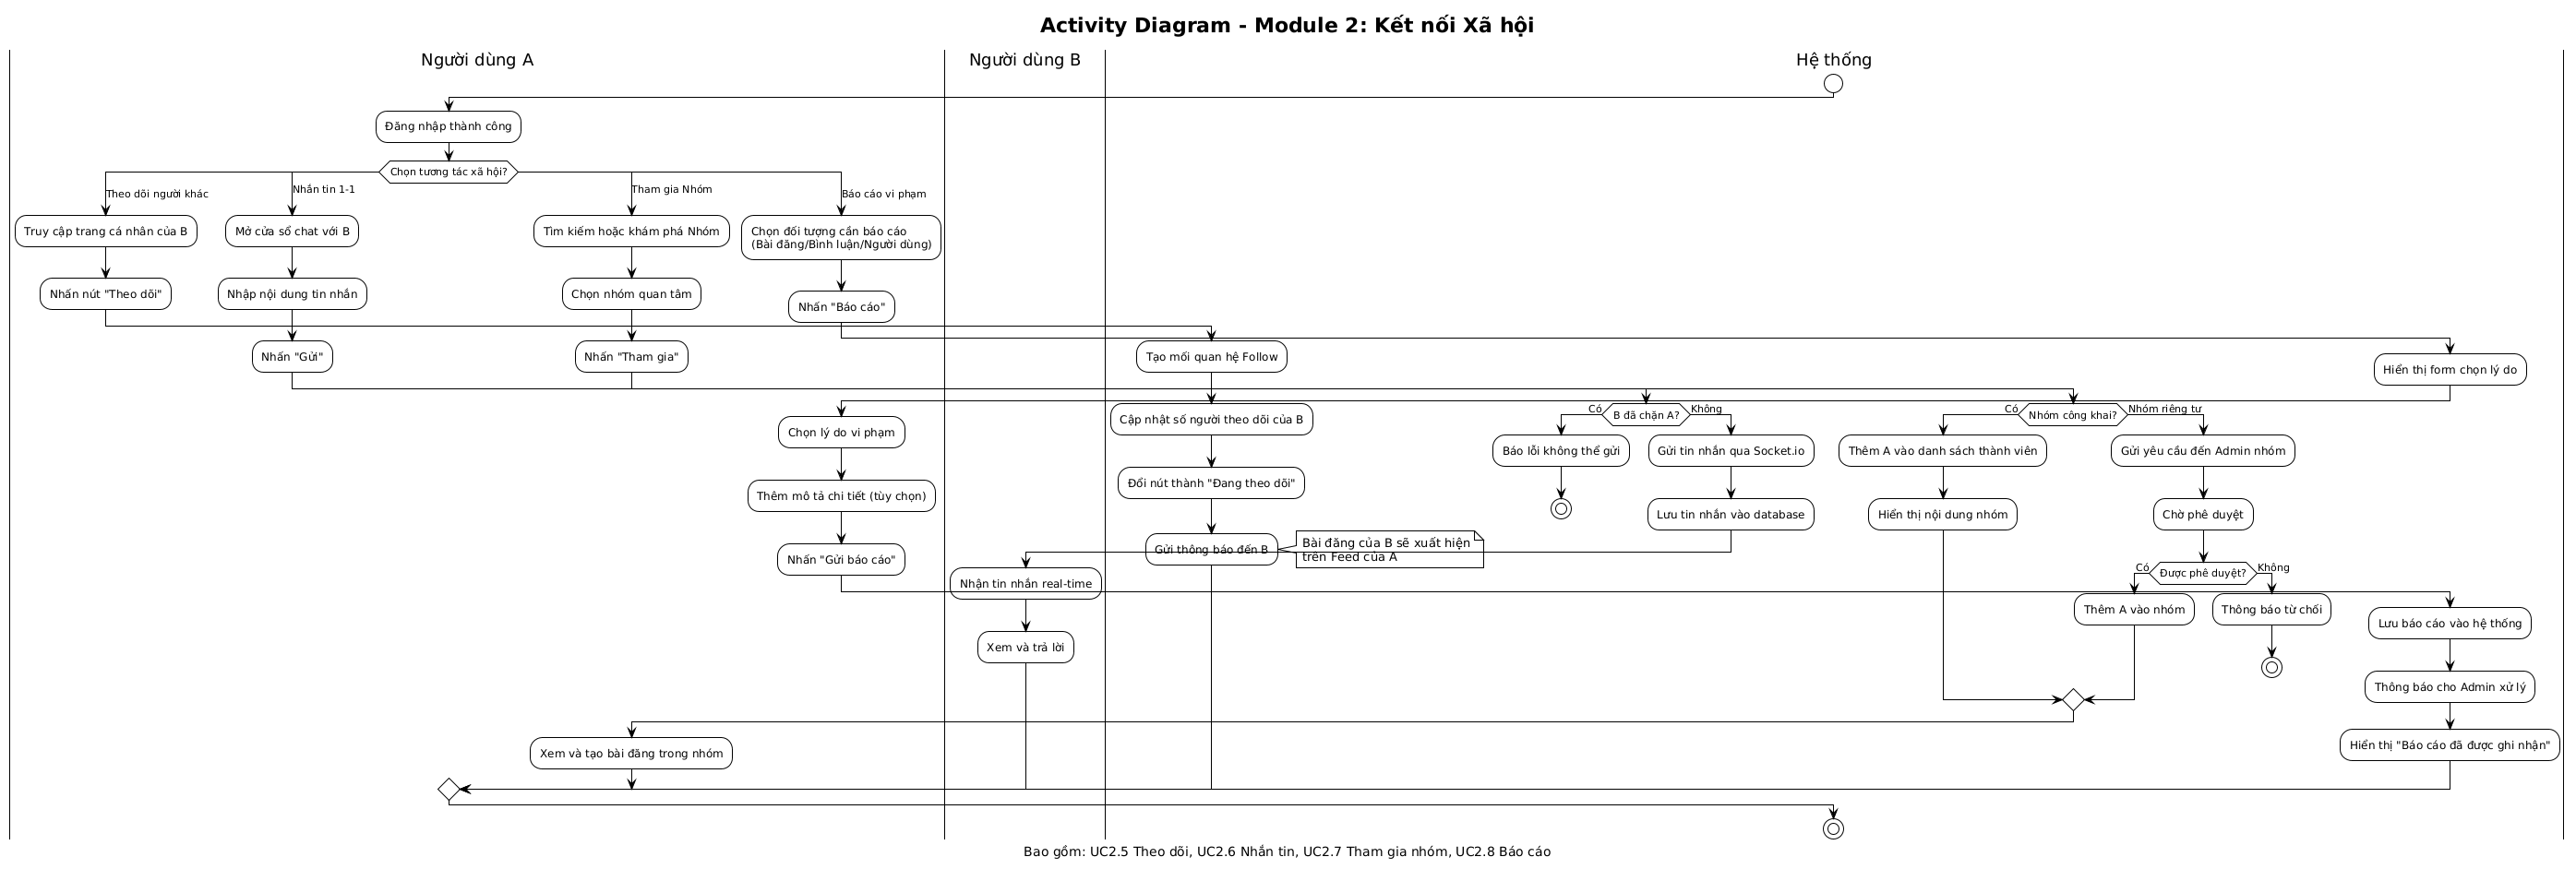
\includegraphics[width=\textwidth]{Images/Activity diagrams/AD-M2-SocialConnections.png}
  \caption{Activity Diagram - Kết nối Xã hội (AD-M2-SocialConnections)}
\end{figure}

\subsection{Module 3 – Commerce}

Module này bao quát hệ sinh thái thương mại điện tử: hành trình mua hàng của Buyer (tìm kiếm, xem sản phẩm, giỏ hàng, thanh toán, theo dõi đơn hàng, đánh giá) và quản lý của Seller (sản phẩm, đơn hàng, hoàn tiền, phản hồi đánh giá).

\subsubsection{AD-M3-BuyerFlow}

Diagram này mô tả toàn bộ quy trình mua hàng từ góc nhìn của người mua (Buyer).

\textbf{UC3.1 – Tìm kiếm và lọc sản phẩm:} Buyer nhập từ khóa và áp dụng bộ lọc (danh mục, khoảng giá, tags). Hệ thống truy vấn database và hiển thị danh sách sản phẩm phù hợp hoặc thông báo không tìm thấy.

\textbf{UC3.2 – Xem chi tiết sản phẩm và chọn biến thể:} Buyer chọn sản phẩm, hệ thống hiển thị chi tiết (hình ảnh, mô tả, giá, tồn kho, đánh giá). Buyer chọn biến thể (size, màu) và số lượng.

\textbf{UC3.3 – Thêm vào giỏ hàng:} Buyer nhấn "Thêm vào giỏ hàng". Hệ thống kiểm tra tồn kho, nếu còn hàng thì lưu vào giỏ hàng và cập nhật số lượng. Nếu hết hàng, hệ thống trả về lỗi và đề xuất sản phẩm tương tự.

\textbf{UC3.4 – Quản lý giỏ hàng:} Buyer truy cập giỏ hàng, hệ thống hiển thị danh sách sản phẩm và tổng tiền. Buyer có thể cập nhật số lượng hoặc xóa sản phẩm, hệ thống tự động tính lại tổng tiền.

\textbf{UC3.5 – Thanh toán:} Buyer nhấn "Thanh toán". Hệ thống kiểm tra tồn kho lần cuối. Nếu đủ hàng, Buyer nhập địa chỉ giao hàng và chọn phương thức thanh toán. Hệ thống tạo đơn hàng với trạng thái \textit{Processing}, làm rỗng giỏ hàng, gửi thông báo cho Seller và hiển thị "Đặt hàng thành công".

\textbf{UC3.6 – Theo dõi đơn hàng:} Buyer xem "Đơn hàng của tôi", hệ thống hiển thị danh sách đơn hàng với mã, trạng thái và ngày đặt. Buyer có thể xem chi tiết và theo dõi trạng thái real-time.

\textbf{UC3.7 – Đánh giá sản phẩm:} Khi đơn hàng đã giao (\textit{Delivered}), Buyer có thể đánh giá sản phẩm (chọn số sao, viết nhận xét, tải ảnh). Hệ thống lưu đánh giá và hiển thị trên trang chi tiết sản phẩm.

\begin{figure}[H]
  \centering
  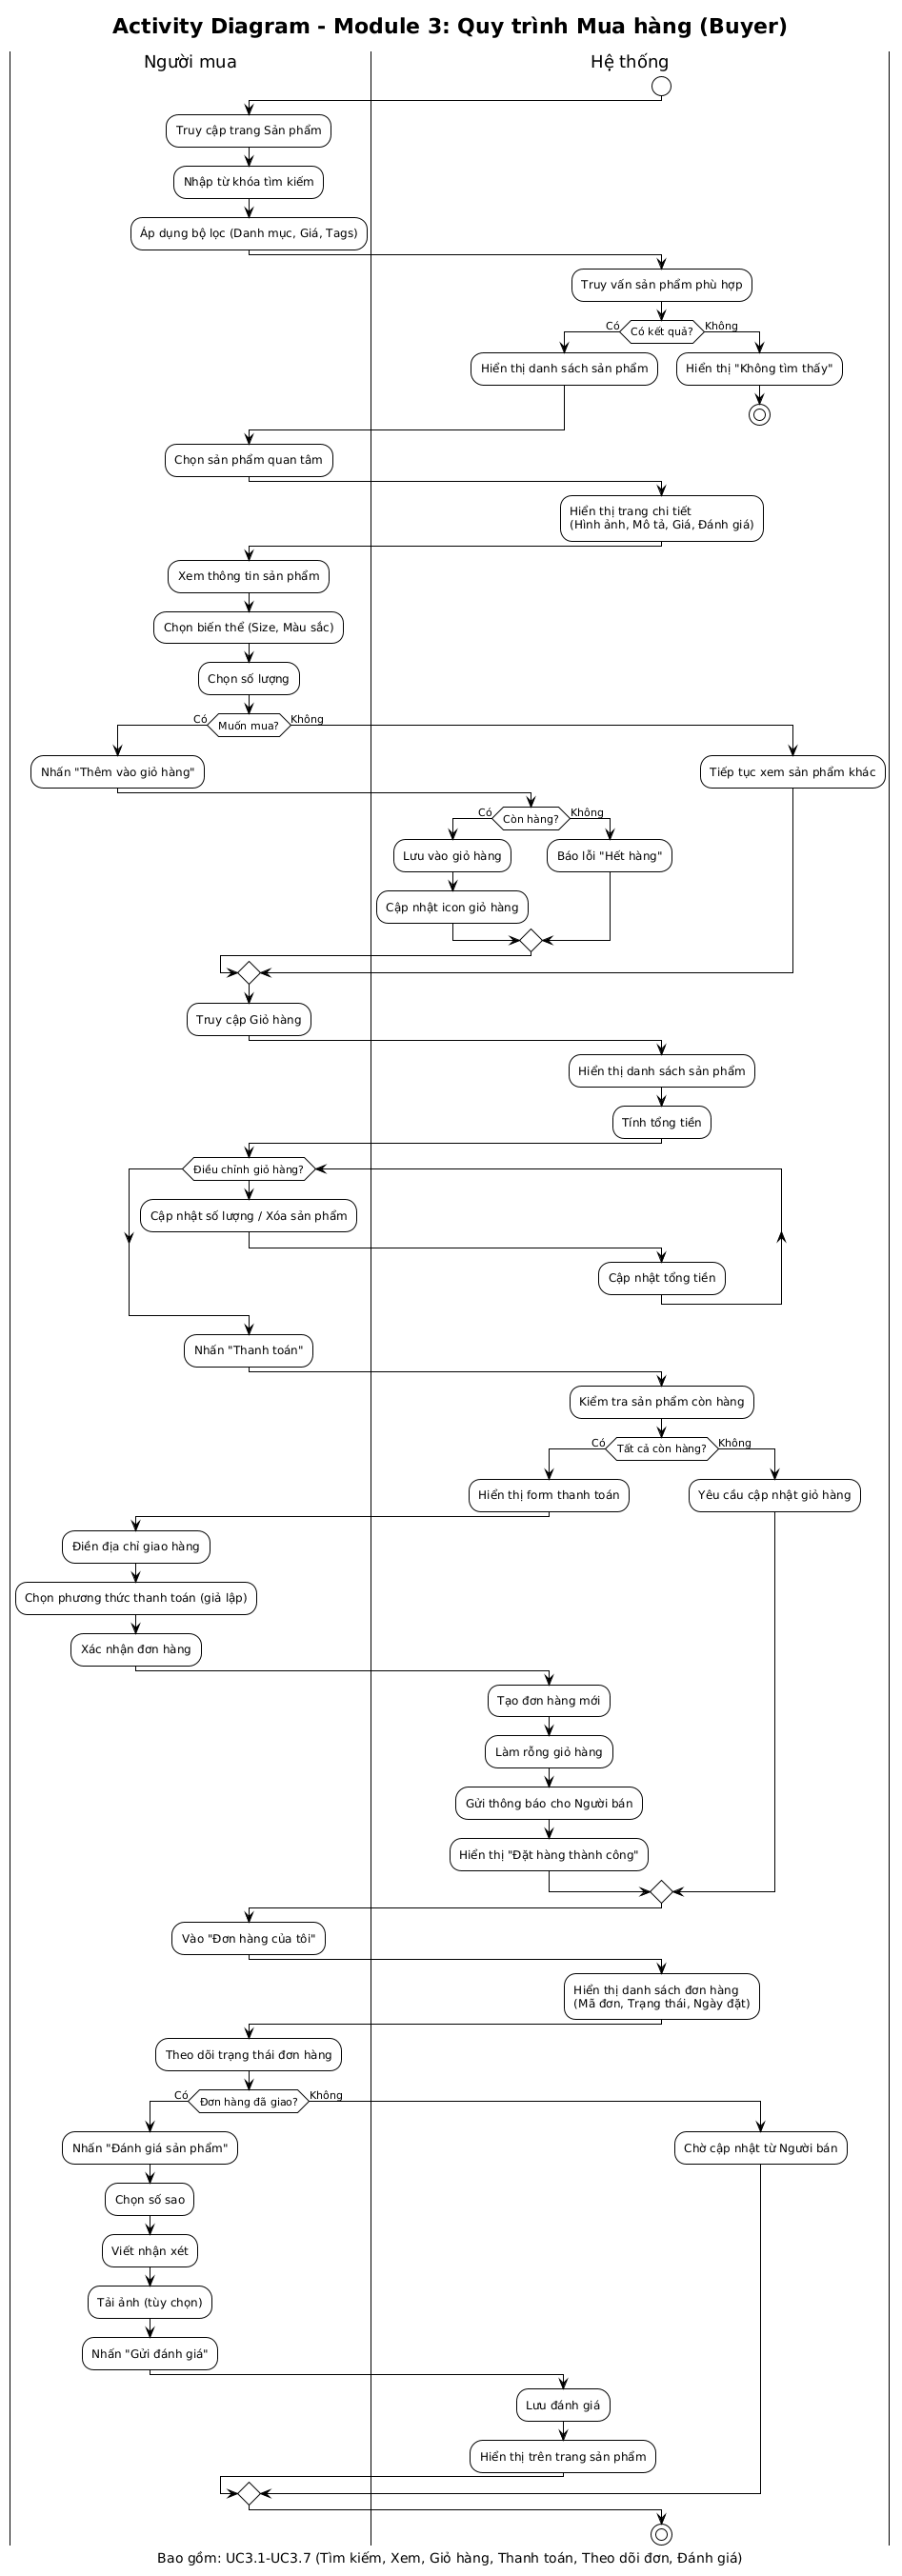
\includegraphics[width=\textwidth]{Images/Activity diagrams/AD-M3-BuyerFlow.png}
  \caption{Activity Diagram - Quy trình Mua hàng (AD-M3-BuyerFlow)}
\end{figure}

\subsubsection{AD-M3-Seller-ProductsOrders}

Diagram này mô tả các tác vụ quản lý sản phẩm và đơn hàng của Seller.

\textbf{UC3.8 – Quản lý sản phẩm:} Seller truy cập Dashboard Bán hàng, chọn "Quản lý Sản phẩm". Seller có thể thêm (tên, mô tả, giá, tồn kho, hình ảnh, biến thể), sửa hoặc xóa sản phẩm (soft delete). Hệ thống xác thực và lưu vào database.

\textbf{UC3.10 – Quản lý đơn hàng:} Seller chọn "Quản lý Đơn hàng", hệ thống hiển thị danh sách đơn hàng. Seller xem chi tiết và cập nhật trạng thái: "Đang xử lý", "Đang giao", "Đã giao", hoặc "Đã hủy". Hệ thống lưu thay đổi, ghi lịch sử và gửi thông báo đến Buyer.

\begin{figure}[H]
  \centering
  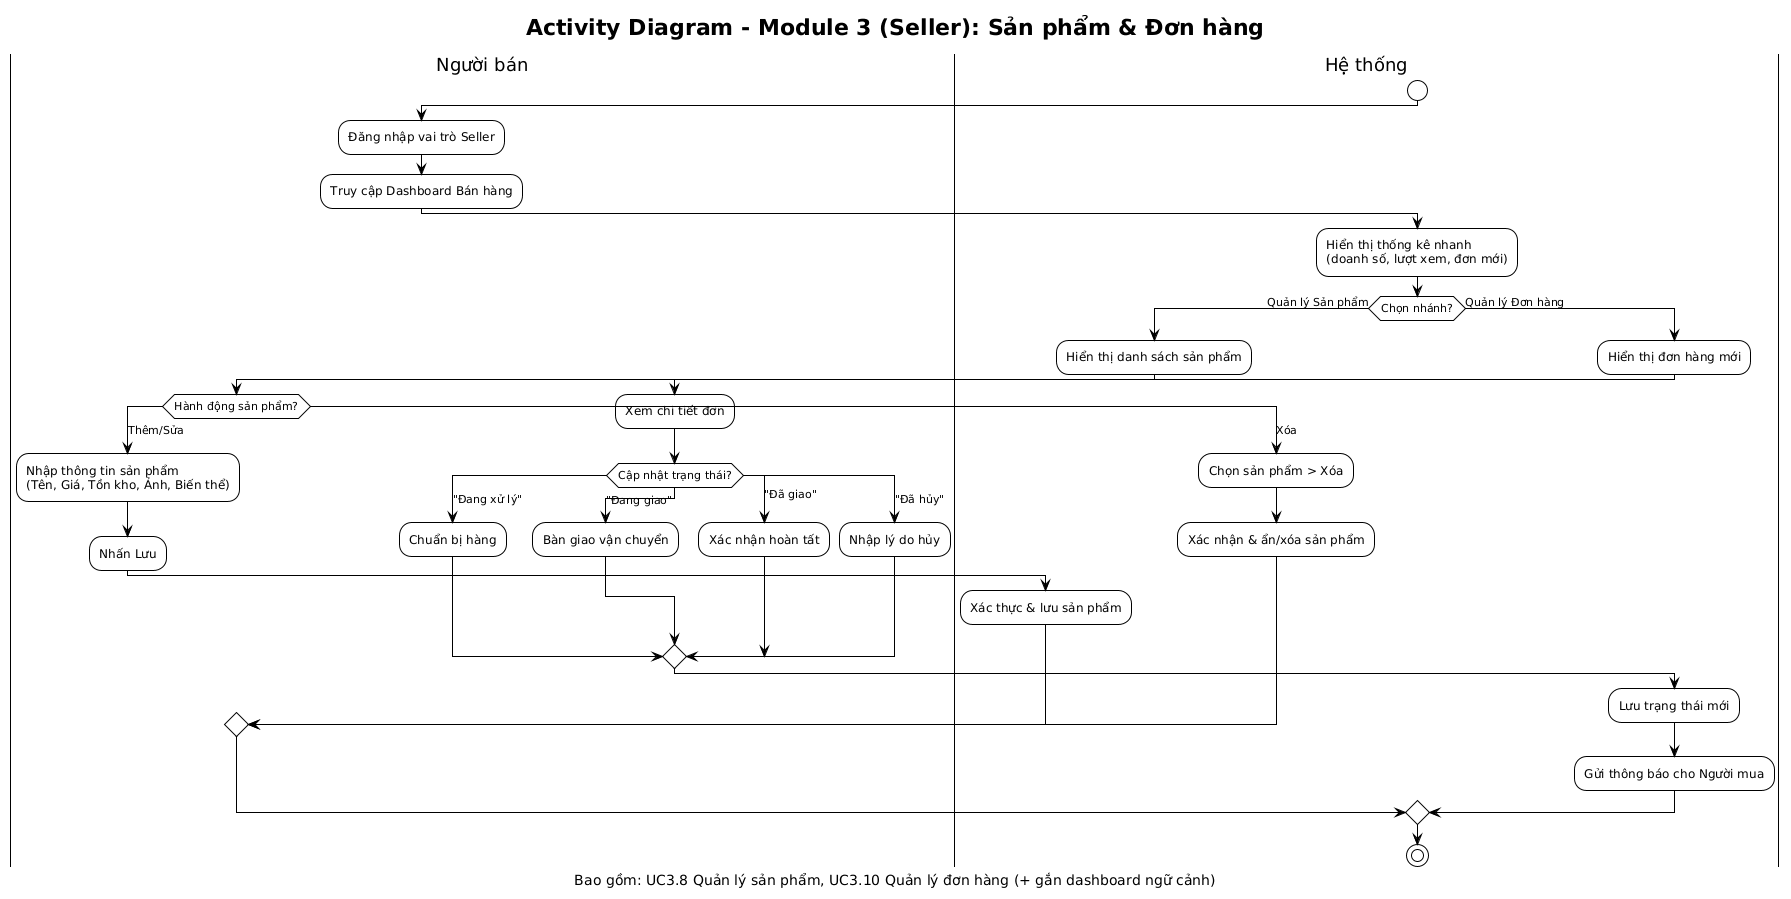
\includegraphics[width=\textwidth]{Images/Activity diagrams/AD-M3-Seller-ProductsOrders.png}
  \caption{Activity Diagram - Quản lý Sản phẩm và Đơn hàng của Seller (AD-M3-Seller-ProductsOrders)}
\end{figure}

\subsubsection{AD-M3-Seller-RefundReview}

Diagram này mô tả quy trình xử lý hoàn tiền và phản hồi đánh giá của Seller.

\textbf{UC3.11 – Xử lý hoàn tiền:} Seller chọn "Xử lý hoàn tiền", hệ thống hiển thị danh sách yêu cầu hoàn tiền. Seller xem chi tiết và quyết định chấp nhận hoặc từ chối. Nếu chấp nhận, hệ thống cập nhật trạng thái \textit{Refunded}, xử lý hoàn tiền và gửi thông báo. Nếu từ chối, hệ thống lưu lý do và gửi thông báo đến Buyer.

\textbf{UC3.12 – Phản hồi đánh giá:} Seller chọn "Đánh giá", hệ thống hiển thị danh sách đánh giá từ Buyer. Seller chọn đánh giá cần phản hồi, nhập nội dung và gửi. Hệ thống lưu phản hồi và hiển thị dưới đánh giá gốc trên trang sản phẩm.

\begin{figure}[H]
  \centering
  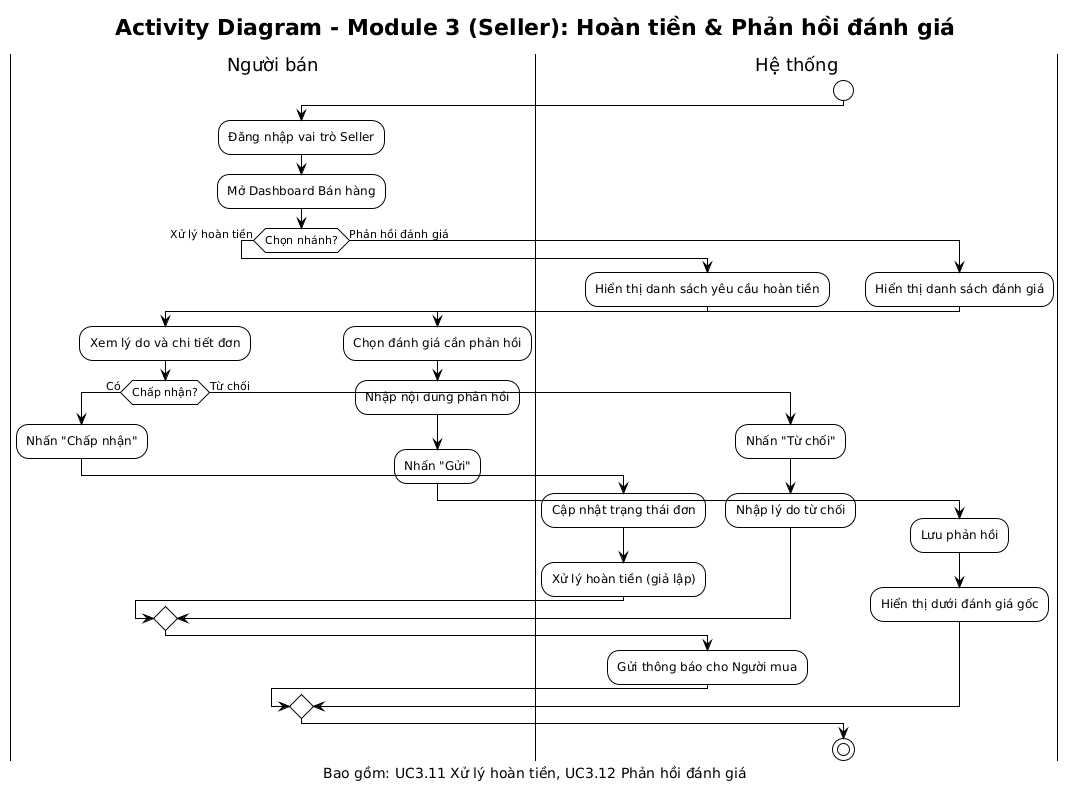
\includegraphics[width=\textwidth]{Images/Activity diagrams/AD-M3-Seller-RefundReview.png}
  \caption{Activity Diagram - Hoàn tiền và Phản hồi Đánh giá của Seller (AD-M3-Seller-RefundReview)}
\end{figure}

\subsection{Module 4 – Admin}

Module này cung cấp công cụ quản trị: quản lý tài khoản (vô hiệu hóa, kích hoạt, thay đổi vai trò), quản lý nội dung (duyệt và xóa bài đăng, sản phẩm vi phạm), xử lý báo cáo vi phạm, và thống kê tổng quan hệ thống.

\subsubsection{AD-M4-Admin-AccountsContent}

Diagram này mô tả quy trình quản lý tài khoản người dùng và nội dung của Admin.

\textbf{UC4.1 – Quản lý tài khoản:} Admin chọn "Quản lý Tài khoản", hệ thống hiển thị danh sách người dùng. Admin có thể tìm kiếm/lọc theo tên, email, vai trò, trạng thái. Admin có thể vô hiệu hóa, kích hoạt lại, hoặc đổi vai trò người dùng. Mỗi hành động được ghi lịch sử và cập nhật database.

\textbf{UC4.2 – Quản lý nội dung:} Admin chọn "Quản lý Nội dung", hệ thống hiển thị danh sách bài đăng và sản phẩm (có thể lọc theo loại, người đăng, trạng thái). Admin xem chi tiết và có thể xóa nội dung vi phạm. Hệ thống xóa/ẩn nội dung và gửi email thông báo đến chủ sở hữu.

\begin{figure}[H]
  \centering
  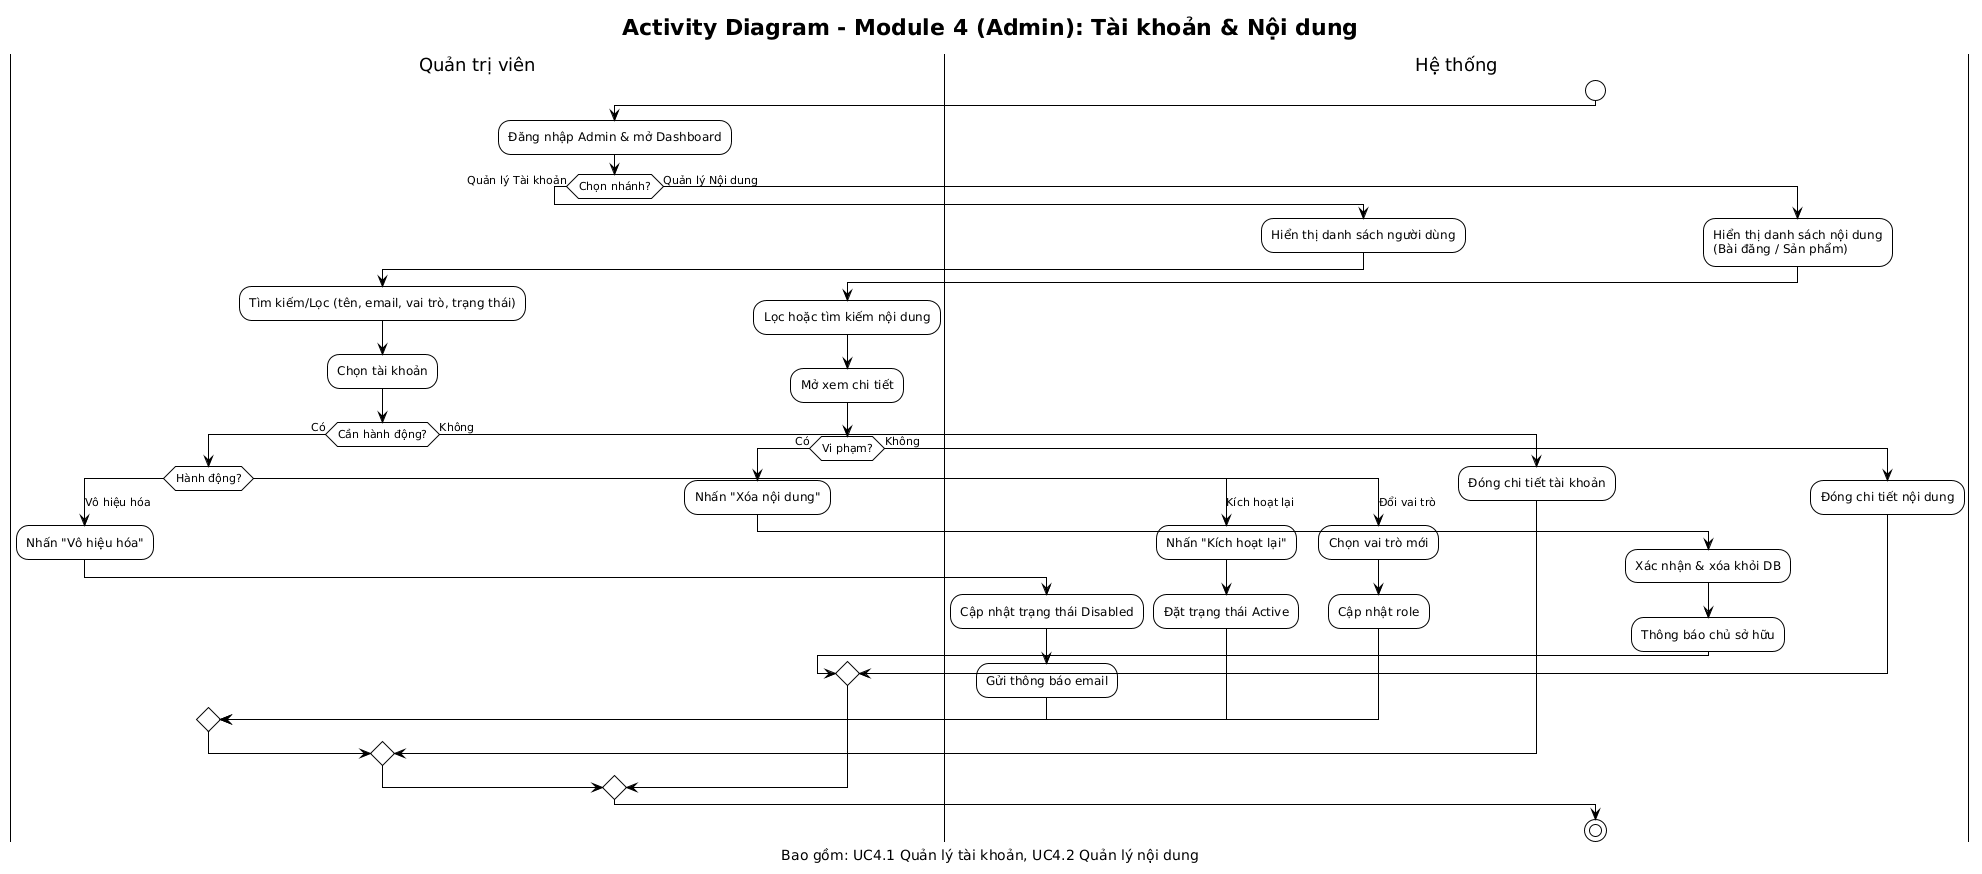
\includegraphics[width=\textwidth]{Images/Activity diagrams/AD-M4-Admin-AccountsContent.png}
  \caption{Activity Diagram - Quản lý Tài khoản và Nội dung của Admin (AD-M4-Admin-AccountsContent)}
\end{figure}

\subsubsection{AD-M4-Admin-ReportsAnalytics}

Diagram này mô tả quy trình xử lý báo cáo vi phạm và xem thống kê phân tích của Admin.

\textbf{UC4.3 – Xử lý báo cáo vi phạm:} Admin chọn "Xử lý báo cáo vi phạm", hệ thống hiển thị danh sách báo cáo đang chờ (sắp xếp theo mức độ ưu tiên). Admin xem chi tiết và đánh giá tính hợp lệ. Nếu hợp lệ, Admin chọn hành động: xóa nội dung, khóa tài khoản, hoặc gửi cảnh cáo. Hệ thống thực thi hành động, đánh dấu "Đã xử lý" và gửi thông báo. Nếu không hợp lệ, Admin đánh dấu "Từ chối".

\textbf{UC4.4 – Thống kê và phân tích:} Admin chọn khoảng thời gian và xem Dashboard với các chỉ số: số lượng người dùng (mới, tổng), tỷ lệ Buyer/Seller, số lượng bài đăng/sản phẩm mới, hoạt động giao dịch (đơn hàng, doanh thu). Dashboard có biểu đồ trực quan hóa xu hướng theo thời gian.

\begin{figure}[H]
  \centering
  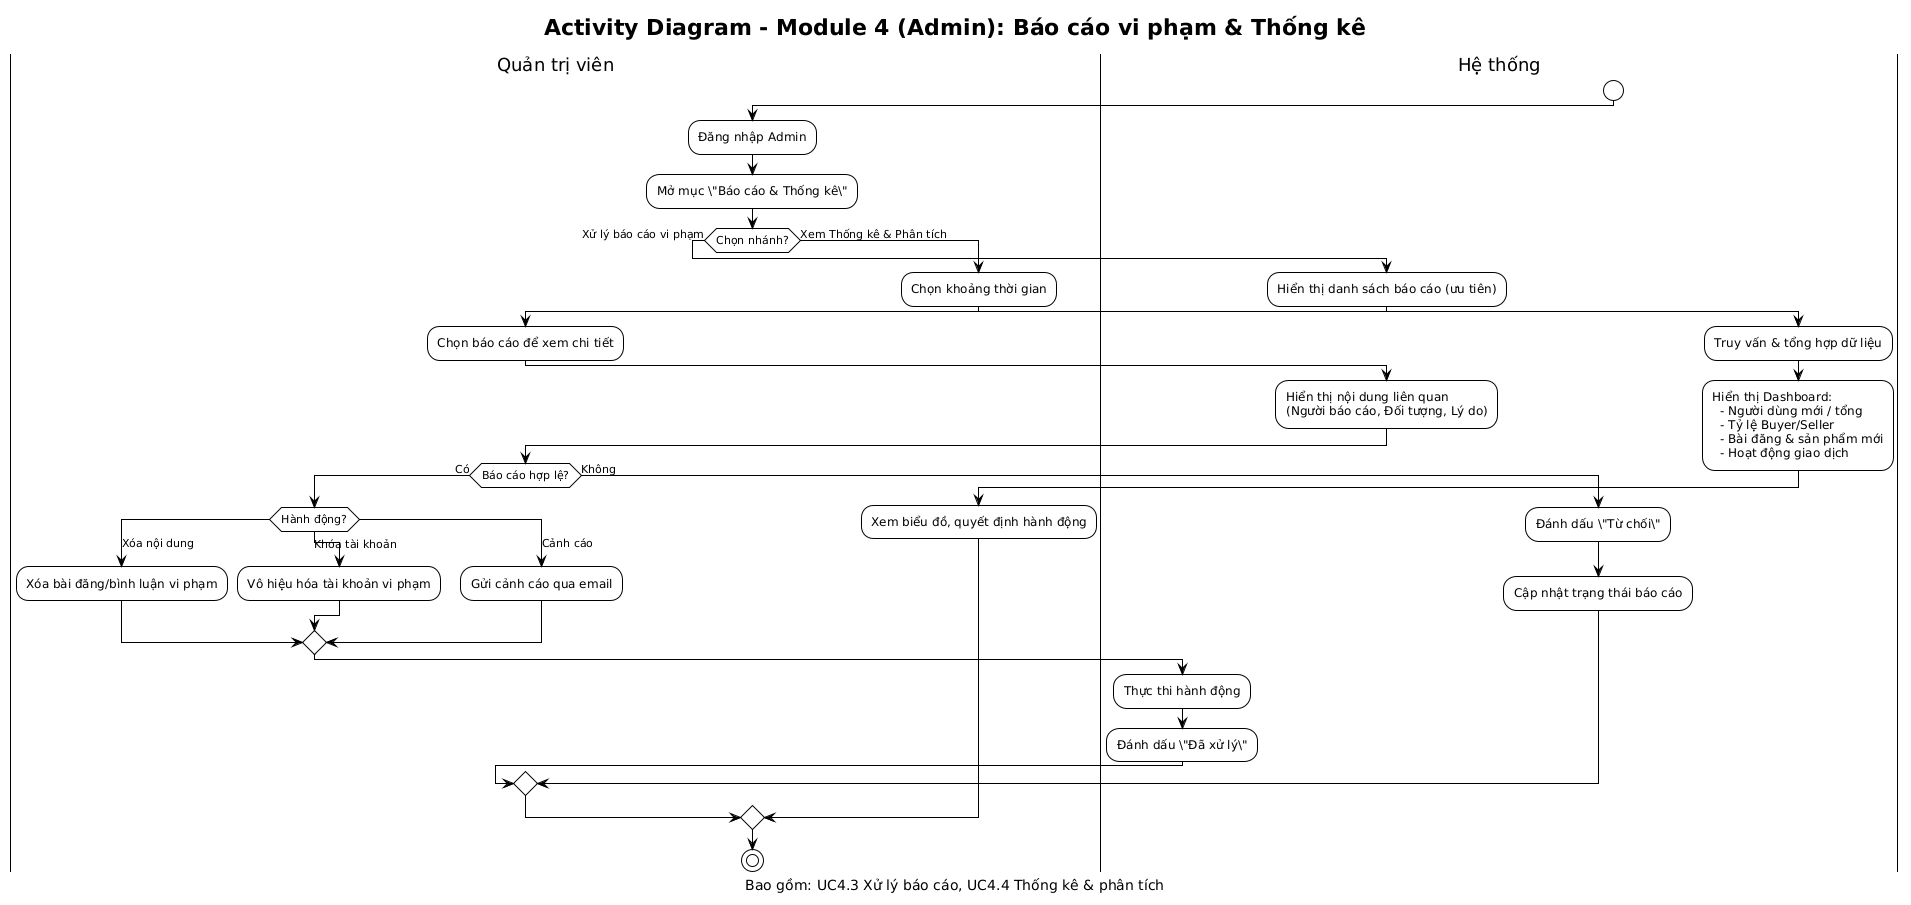
\includegraphics[width=\textwidth]{Images/Activity diagrams/AD-M4-Admin-ReportsAnalytics.png}
  \caption{Activity Diagram - Báo cáo và Thống kê của Admin (AD-M4-Admin-ReportsAnalytics)}
\end{figure}

\subsection{Module 5 – AI Content Assistant}

Module này tích hợp AI (Google Gemini API) để hỗ trợ tạo nội dung đa phương thức: generate text, generate image+text, và generate video+images+text. Luồng xử lý được thiết kế theo mô hình \textbf{Evaluate--Refine Loop}: sau khi gọi API tạo nội dung, hệ thống tự động đánh giá chất lượng kết quả dựa trên các tiêu chí đã định nghĩa. Nếu điểm đánh giá chưa đạt ngưỡng ($< 7.0/10$), hệ thống phân tích tiêu chí yếu, bổ sung ràng buộc vào prompt và gọi lại API (tối đa 3 lần). Kết quả tốt nhất được trả về cho người dùng kèm điểm đánh giá chi tiết và gợi ý chỉnh sửa.

\subsubsection{AD-M5-UC5.1-GenerateText}

Diagram này mô tả quy trình tạo nội dung bài đăng từ mô tả, ý tưởng và hình ảnh sản phẩm sử dụng Google Gemini API, bao gồm vòng lặp đánh giá và cải thiện tự động.

\textbf{UC5.1 – Tạo bài viết từ mô tả, ý tưởng và hình ảnh sản phẩm:} Người dùng nhập mô tả/ý tưởng và tải hình ảnh sản phẩm (nếu có), nhấn ``Tạo bài viết với AI''. Hệ thống thực hiện quy trình sau:

\begin{enumerate}
    \item \textbf{Phân tích đầu vào}: Trích xuất thực thể chính (tên sản phẩm, đặc điểm, lợi ích), xác định giọng điệu và phân loại loại nội dung (quảng cáo, chia sẻ, giáo dục). Nếu có hình ảnh, sử dụng Gemini Vision phân tích nội dung hình.
    \item \textbf{Xây dựng Prompt}: Tổng hợp thông tin vào prompt có cấu trúc 5 phần (System Instruction, Context, User Input, Constraints, Output Format). Ràng buộc bao gồm: độ dài 100--300 từ, 5--10 hashtag, phải có Call-to-Action, output dạng JSON.
    \item \textbf{Gọi API}: Gửi prompt đến Google Gemini API.
    \item \textbf{Đánh giá chất lượng}: Kết quả được chấm điểm theo 6 tiêu chí: Tính liên quan (0.25), Tính hấp dẫn (0.20), Cấu trúc hoàn chỉnh (0.15), Độ dài phù hợp (0.10), Chất lượng ngôn ngữ (0.15), Giá trị thương mại (0.15). Điểm tổng hợp là trung bình có trọng số.
    \item \textbf{Quyết định}: Nếu điểm $\geq$ 7.0 $\rightarrow$ trả kết quả. Nếu $<$ 7.0 và chưa đạt giới hạn 3 lần thử $\rightarrow$ xác định tiêu chí yếu, bổ sung ràng buộc vào prompt, gọi lại API. Nếu đã hết lần thử $\rightarrow$ trả kết quả tốt nhất kèm gợi ý chỉnh sửa.
    \item \textbf{Hiển thị}: Bài viết được chèn vào trình soạn thảo kèm điểm đánh giá chi tiết. Người dùng có thể chỉnh sửa trực tiếp, yêu cầu viết lại đoạn cụ thể, thay đổi giọng điệu, hoặc tạo lại toàn bộ.
\end{enumerate}

\begin{figure}[H]
  \centering
  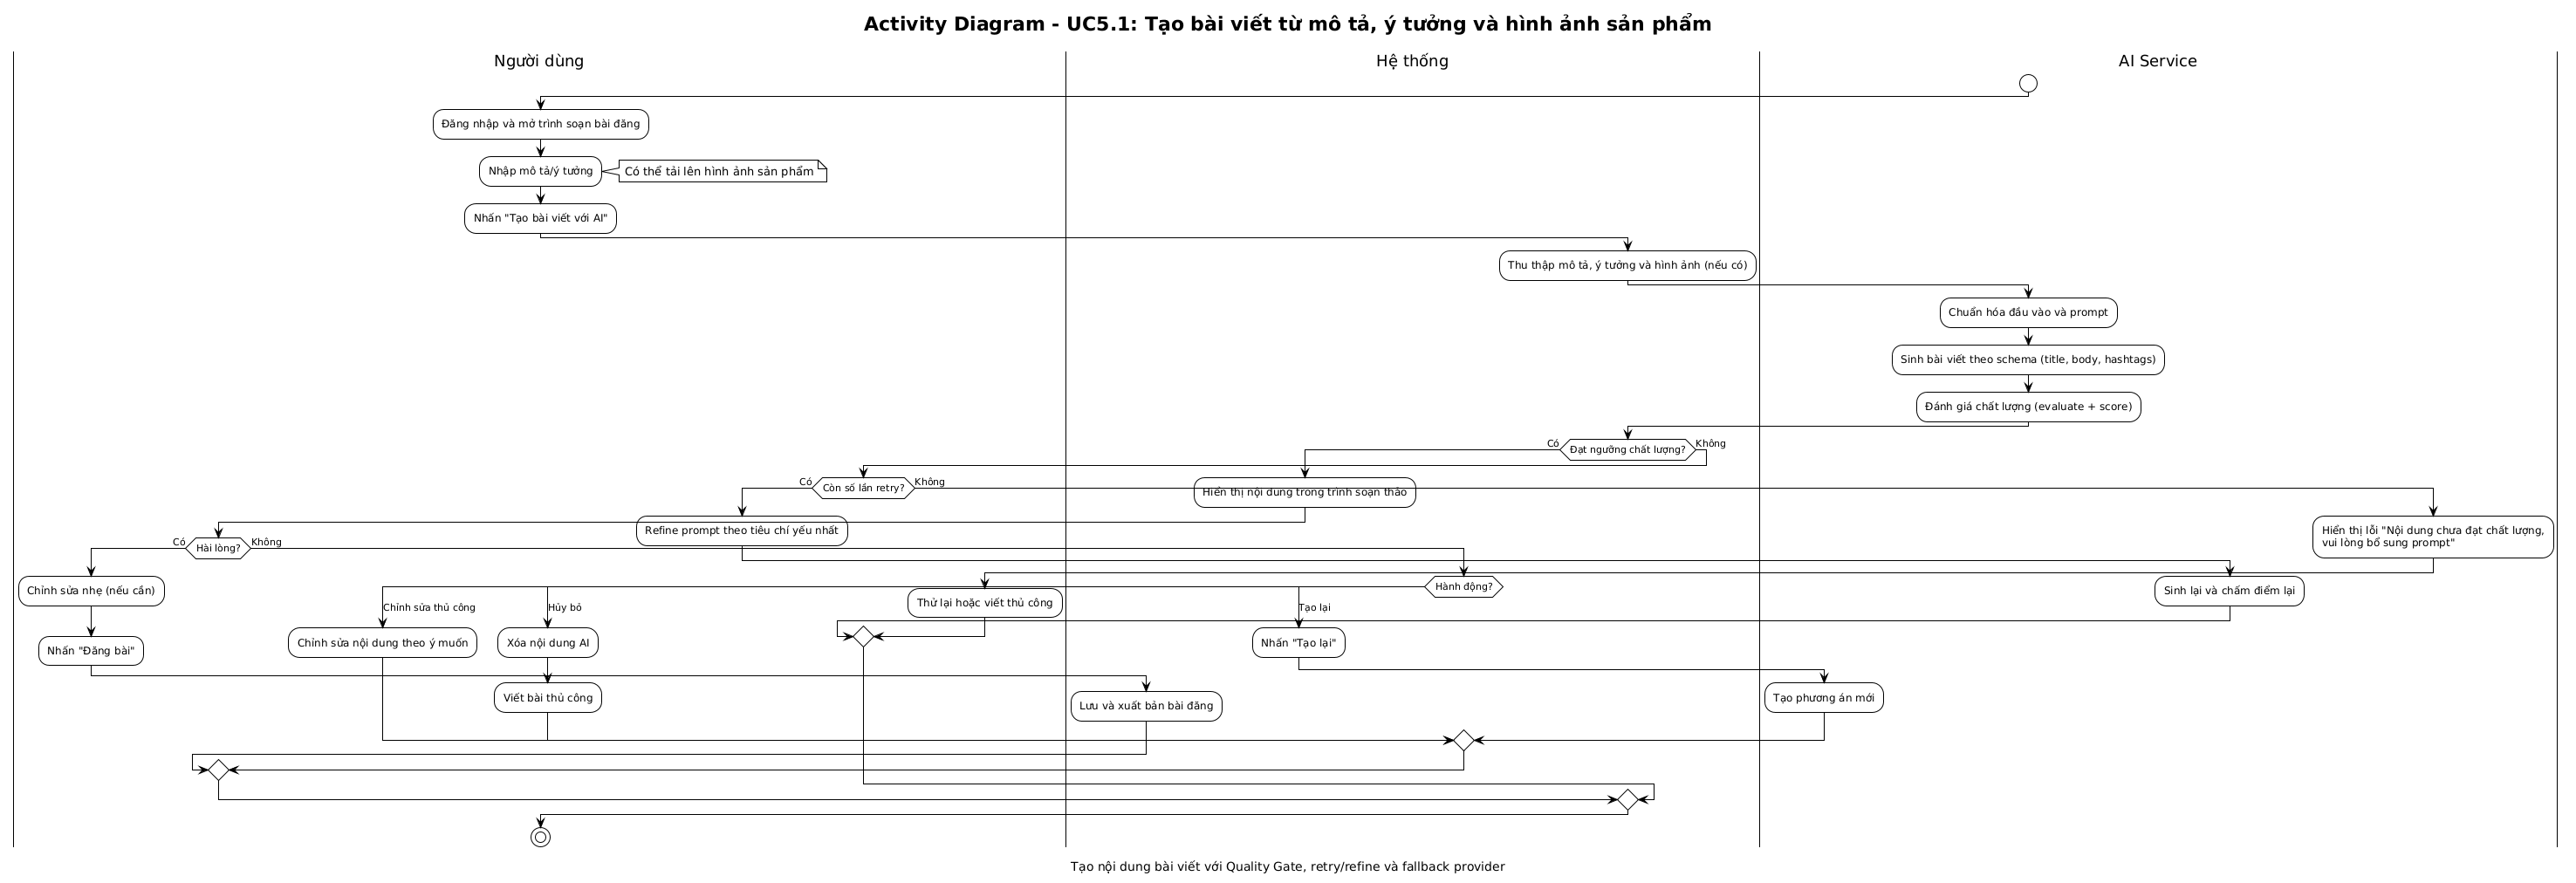
\includegraphics[width=\textwidth]{Images/Activity diagrams/AD-M5-UC5.1-GenerateText.png}
  \caption{Activity Diagram - Tạo bài viết với vòng lặp đánh giá và cải thiện (AD-M5-UC5.1-GenerateText)}
\end{figure}

\subsubsection{AD-M5-UC5.2-GenerateImageText}

Diagram này mô tả quy trình tạo bài viết và hình ảnh từ mô tả, ý tưởng và hình ảnh đầu vào sử dụng Google Gemini API, với đánh giá chất lượng riêng biệt cho text và image.

\textbf{UC5.2 – Tạo bài viết và hình ảnh:} Người dùng nhập mô tả/ý tưởng và hình ảnh đầu vào (nếu có), nhấn ``Tạo bài viết và hình ảnh với AI''. Hệ thống thực hiện quy trình sau:

\begin{enumerate}
    \item \textbf{Phân tích đầu vào}: Tương tự UC5.1, bổ sung phân tích hình ảnh đầu vào để xác định phong cách hình ảnh (màu sắc chủ đạo, bố cục, đối tượng).
    \item \textbf{Xây dựng Prompt kép}: Tạo prompt cho text (tương tự UC5.1) và prompt riêng cho image (bao gồm Visual Spec, phong cách, tỷ lệ 1:1 hoặc 4:5, negative prompt). Nội dung text vừa tạo được dùng làm context cho prompt image.
    \item \textbf{Gọi API}: Gửi prompt text đến Gemini API, sau đó sử dụng kết quả text làm context gửi prompt image.
    \item \textbf{Đánh giá chất lượng}: Text được đánh giá theo 6 tiêu chí (như UC5.1). Image được đánh giá theo 4 tiêu chí riêng: Tính liên quan (0.30), Chất lượng kỹ thuật (0.25), Tính thẩm mỹ (0.25), Nhất quán thương hiệu (0.20). Cả hai phải đạt ngưỡng $\geq$ 7.0/10.
    \item \textbf{Quyết định}: Nếu cả text và image đạt $\rightarrow$ trả kết quả. Nếu chỉ một phần chưa đạt $\rightarrow$ chỉ sửa prompt và tạo lại phần chưa đạt (không cần tạo lại phần đã tốt). Nếu hết lần thử $\rightarrow$ trả kết quả tốt nhất.
    \item \textbf{Hiển thị}: Bài viết và hình ảnh được hiển thị trong trình soạn thảo kèm điểm đánh giá từng loại. Người dùng có thể chỉnh sửa text, tạo lại hình ảnh với phong cách khác, hoặc tải lên hình ảnh thay thế.
\end{enumerate}

\begin{figure}[H]
  \centering
  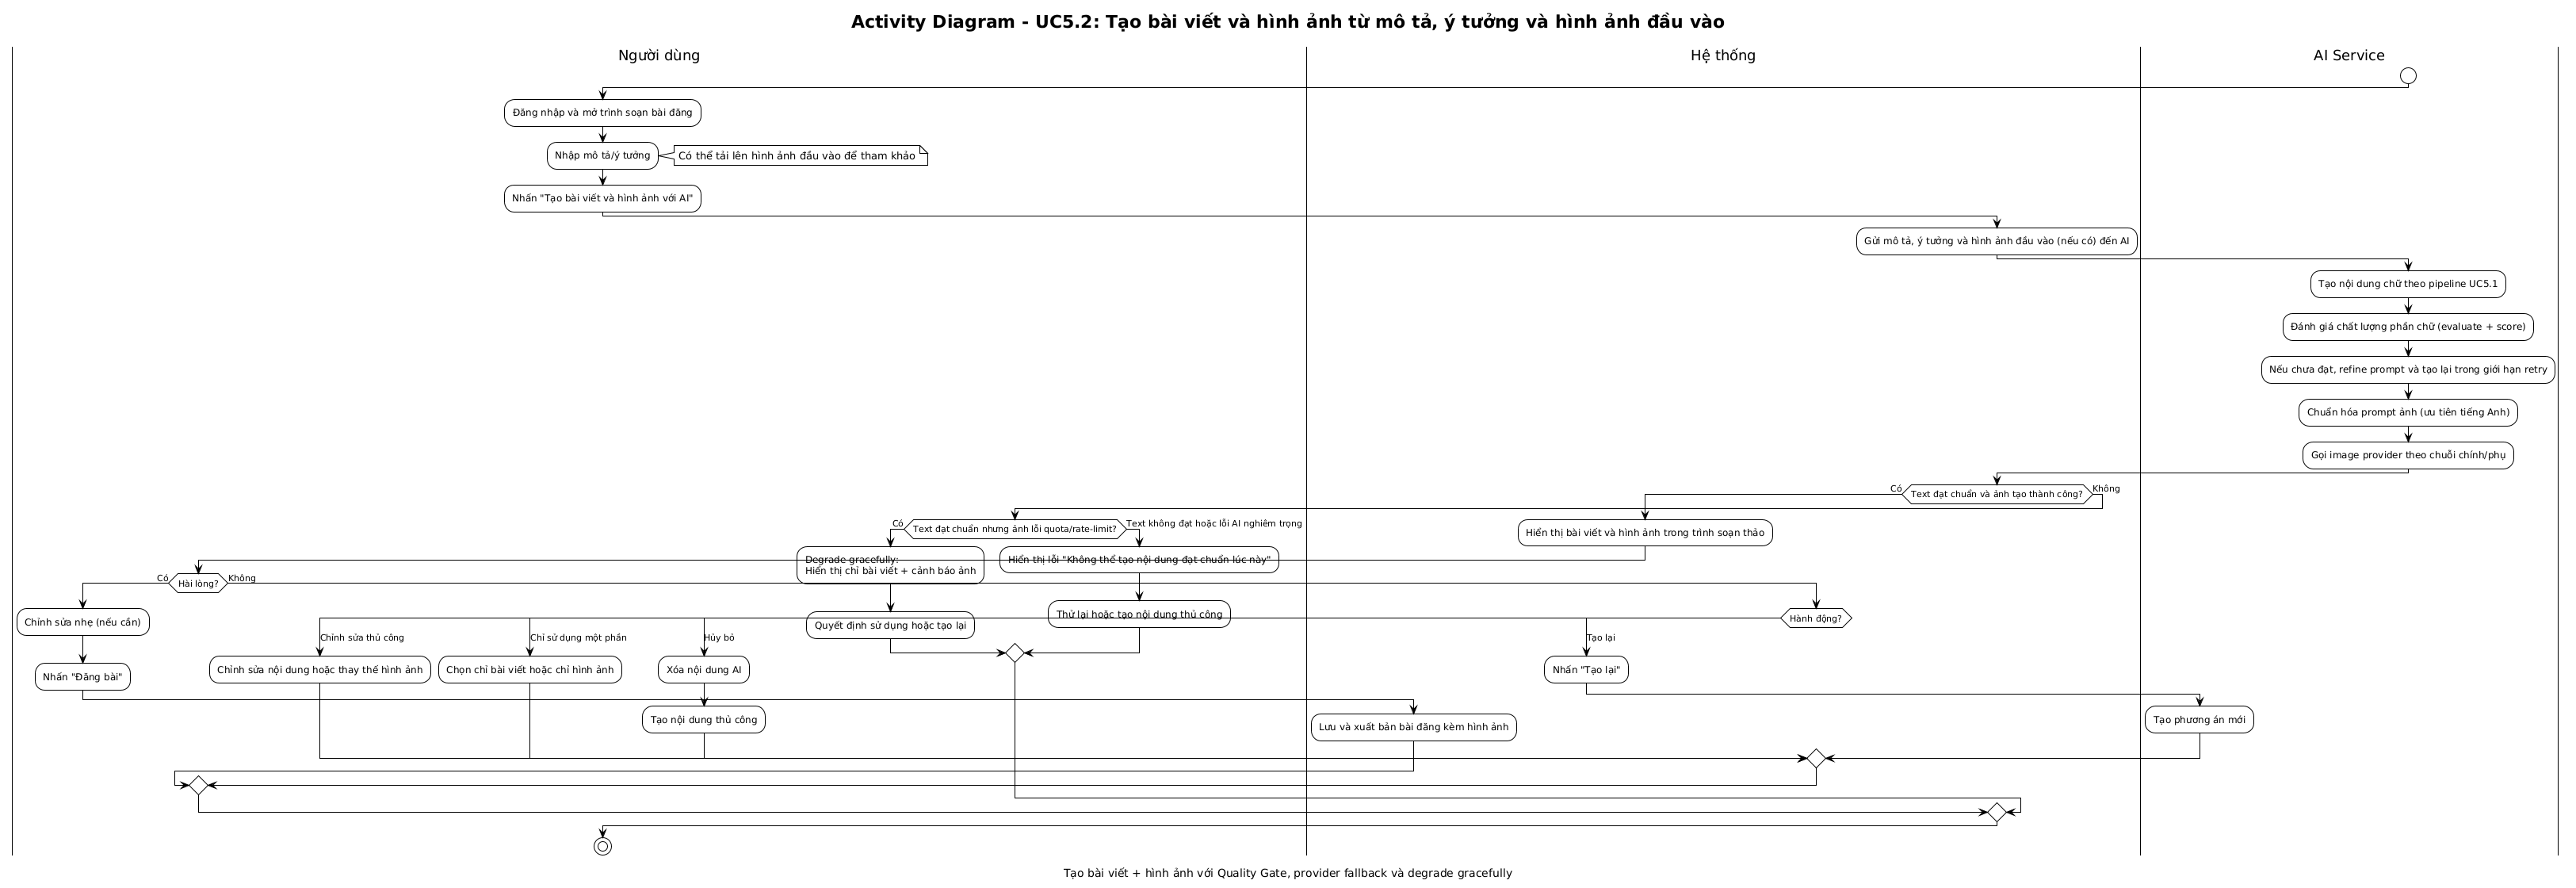
\includegraphics[width=\textwidth]{Images/Activity diagrams/AD-M5-UC5.2-GenerateImageText.png}
  \caption{Activity Diagram - Tạo bài viết và hình ảnh với đánh giá chất lượng riêng biệt (AD-M5-UC5.2-GenerateImageText)}
\end{figure}

\subsubsection{AD-M5-UC5.3-GenerateVideoImagesText}

Diagram này mô tả quy trình tạo nội dung đa phương thức (video + hình ảnh + bài viết) với pipeline đánh giá ba tầng.

\textbf{UC5.3 – Tạo video ngắn, hình ảnh và bài viết:} Người dùng nhập mô tả/ý tưởng và hình ảnh đầu vào (nếu có), nhấn ``Tạo video và nội dung đa phương thức với AI''. Hệ thống thực hiện quy trình sau:

\begin{enumerate}
    \item \textbf{Phân tích đầu vào}: Tương tự UC5.2, bổ sung xác định cấu trúc storyboard cho video (cảnh mở đầu, giới thiệu sản phẩm, highlight, CTA).
    \item \textbf{Xây dựng Prompt ba tầng}: Tạo prompt text $\rightarrow$ dùng text làm context tạo prompt image $\rightarrow$ dùng text + image làm context tạo prompt video. Prompt video bao gồm storyboard tự động, ràng buộc 15--30 giây, tỷ lệ 9:16 hoặc 1:1.
    \item \textbf{Gọi API tuần tự}: Gemini API cho text $\rightarrow$ Gemini API cho images (tối đa 3) $\rightarrow$ Google Veo 2 cho video.
    \item \textbf{Đánh giá chất lượng ba tầng}: Text (6 tiêu chí), Image (4 tiêu chí), Video (5 tiêu chí: Tính mạch lạc 0.25, Chất lượng hình ảnh 0.25, Độ dài phù hợp 0.15, Tính hấp dẫn 0.20, Nhất quán nội dung 0.15). Mỗi loại phải đạt $\geq$ 7.0/10.
    \item \textbf{Quyết định cải thiện có chọn lọc}: Chỉ tạo lại thành phần chưa đạt. Ví dụ: text và image đạt nhưng video chưa đạt $\rightarrow$ chỉ sửa prompt video và tạo lại video, giữ nguyên text và image. Tối đa 3 lần thử cho mỗi thành phần.
    \item \textbf{Hiển thị}: Video, hình ảnh và bài viết được hiển thị kèm điểm đánh giá từng loại. Người dùng có thể chỉnh sửa từng thành phần riêng biệt, tạo lại chỉ phần không hài lòng, hoặc thay thế bằng nội dung tự tạo.
\end{enumerate}

\begin{figure}[H]
  \centering
  \includegraphics[width=\textwidth]{Images/Activity diagrams/AD-M5-UC5.3-GenerateVideoImagesText.png}
  \caption{Activity Diagram - Tạo nội dung đa phương thức với pipeline đánh giá ba tầng (AD-M5-UC5.3-GenerateVideoImagesText)}
\end{figure}

\subsection{Module 6 – Post Scheduling}

Module này cho phép lên lịch đăng bài trong tương lai, quản lý bài đăng đã lên lịch (xem trước, chỉnh sửa, thay đổi thời gian, đăng ngay, xóa), và tự động xuất bản thông qua cron job.

\subsubsection{AD-M6-PostScheduling}

Diagram này mô tả quy trình lên lịch đăng bài và quản lý bài đăng đã lên lịch.

\textbf{UC6.1 – Lên lịch đăng bài:} Người dùng soạn bài đăng, chọn "Lên lịch" và chọn ngày/giờ xuất bản trong tương lai. Hệ thống kiểm tra thời gian hợp lệ, lưu bài đăng với trạng thái \textit{scheduled} và hiển thị thông báo. Nếu thời gian không hợp lệ, hệ thống báo lỗi.

\textbf{UC6.2 – Quản lý bài đăng đã lên lịch:} Người dùng xem danh sách bài viết chờ xuất bản. Người dùng có thể xem trước, chỉnh sửa nội dung/hình ảnh, thay đổi lịch đăng, đăng ngay, hoặc xóa bài viết. Mỗi hành động được cập nhật trong database ngay lập tức.

\textbf{Cron Job – Xuất bản tự động:} Cron job chạy định kỳ kiểm tra các bài viết có trạng thái \textit{scheduled} và thời gian xuất bản đã đến. Đối với mỗi bài viết đến hạn, cron job thay đổi trạng thái thành \textit{published}, xuất bản lên Feed và gửi thông báo đến tác giả.

\begin{figure}[H]
  \centering
  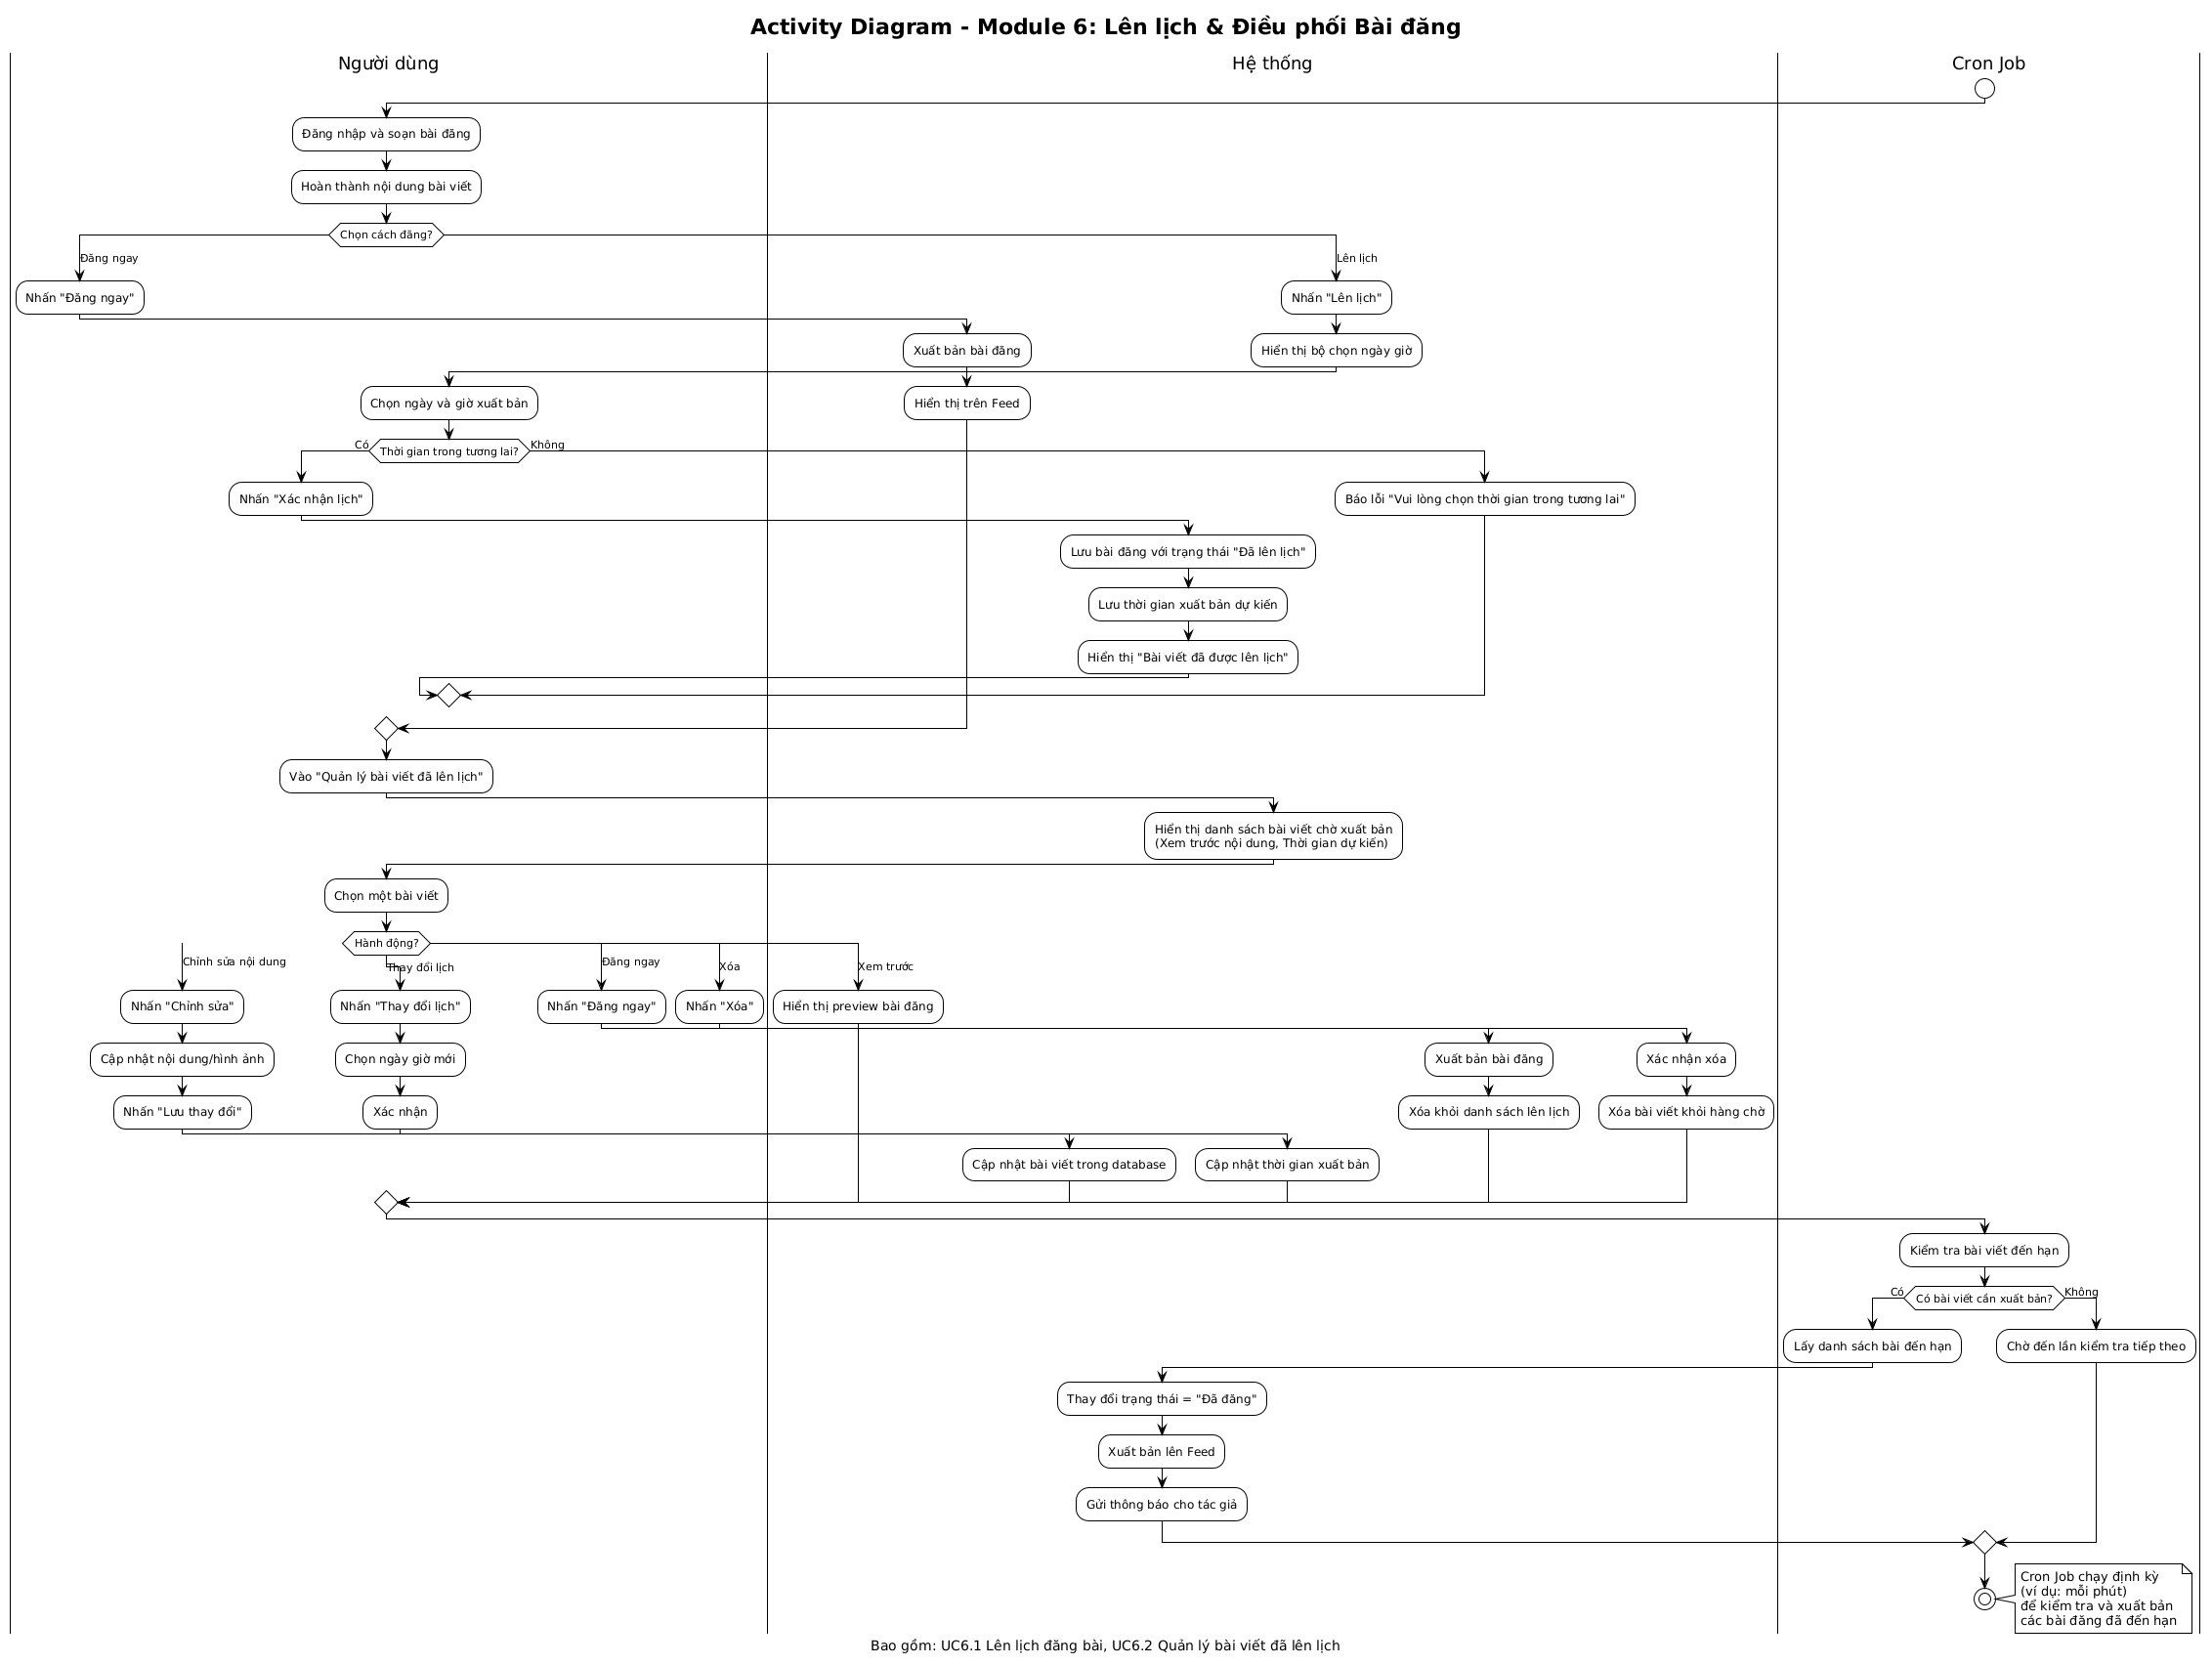
\includegraphics[width=\textwidth]{Images/Activity diagrams/AD-M6-PostScheduling.png}
  \caption{Activity Diagram - Lên lịch và Điều phối Bài đăng (AD-M6-PostScheduling)}
\end{figure}

\subsection{Module 7 – Notification}

Module này cung cấp hệ thống thông báo cho sự kiện tương tác xã hội (like, comment, follow, mention) và giao dịch (đơn hàng, hoàn tiền, đánh giá). Người dùng có thể quản lý thông báo (xem, đánh dấu đã đọc, xóa) và cấu hình nhận thông báo theo loại và kênh (web/email). Sử dụng WebSocket để gửi real-time khi online.

\subsubsection{AD-M7-NotificationSystem}

Diagram này mô tả toàn bộ hệ thống thông báo từ tạo, gửi, quản lý đến cấu hình.

\textbf{UC7.1 – Thông báo tương tác:} Khi A thực hiện tương tác với B (like, comment, follow, mention), hệ thống kiểm tra B có chặn A và cài đặt thông báo của B. Nếu cho phép, hệ thống tạo thông báo và lưu vào database. Nếu B đang online, gửi qua WebSocket ngay lập tức; nếu offline, lưu để hiển thị sau.

\textbf{UC7.2 – Thông báo giao dịch:} Hệ thống tạo và gửi thông báo cho các sự kiện: đơn hàng mới, xác nhận đơn, cập nhật trạng thái giao hàng, yêu cầu hoàn tiền, đánh giá mới. Tất cả thông báo được lưu vào database và gửi real-time nếu người nhận online và bật nhận loại thông báo này.

\textbf{UC7.3 – Quản lý thông báo:} Người dùng mở danh sách thông báo (sắp xếp theo thời gian, mới nhất ở trên). Người dùng có thể xem chi tiết, đánh dấu đã đọc (một hoặc tất cả), xóa một thông báo hoặc xóa tất cả (có xác nhận). Hệ thống cập nhật trạng thái và badge số thông báo chưa đọc.

\textbf{UC7.4 – Cài đặt thông báo:} Người dùng vào Cài đặt > Thông báo, bật/tắt từng loại thông báo (like, comment, follow, đơn hàng, đánh giá, tin nhắn, email) và chọn kênh nhận (web, email, hoặc cả hai). Hệ thống lưu cấu hình vào database và áp dụng ngay lập tức.

\begin{figure}[H]
  \centering
  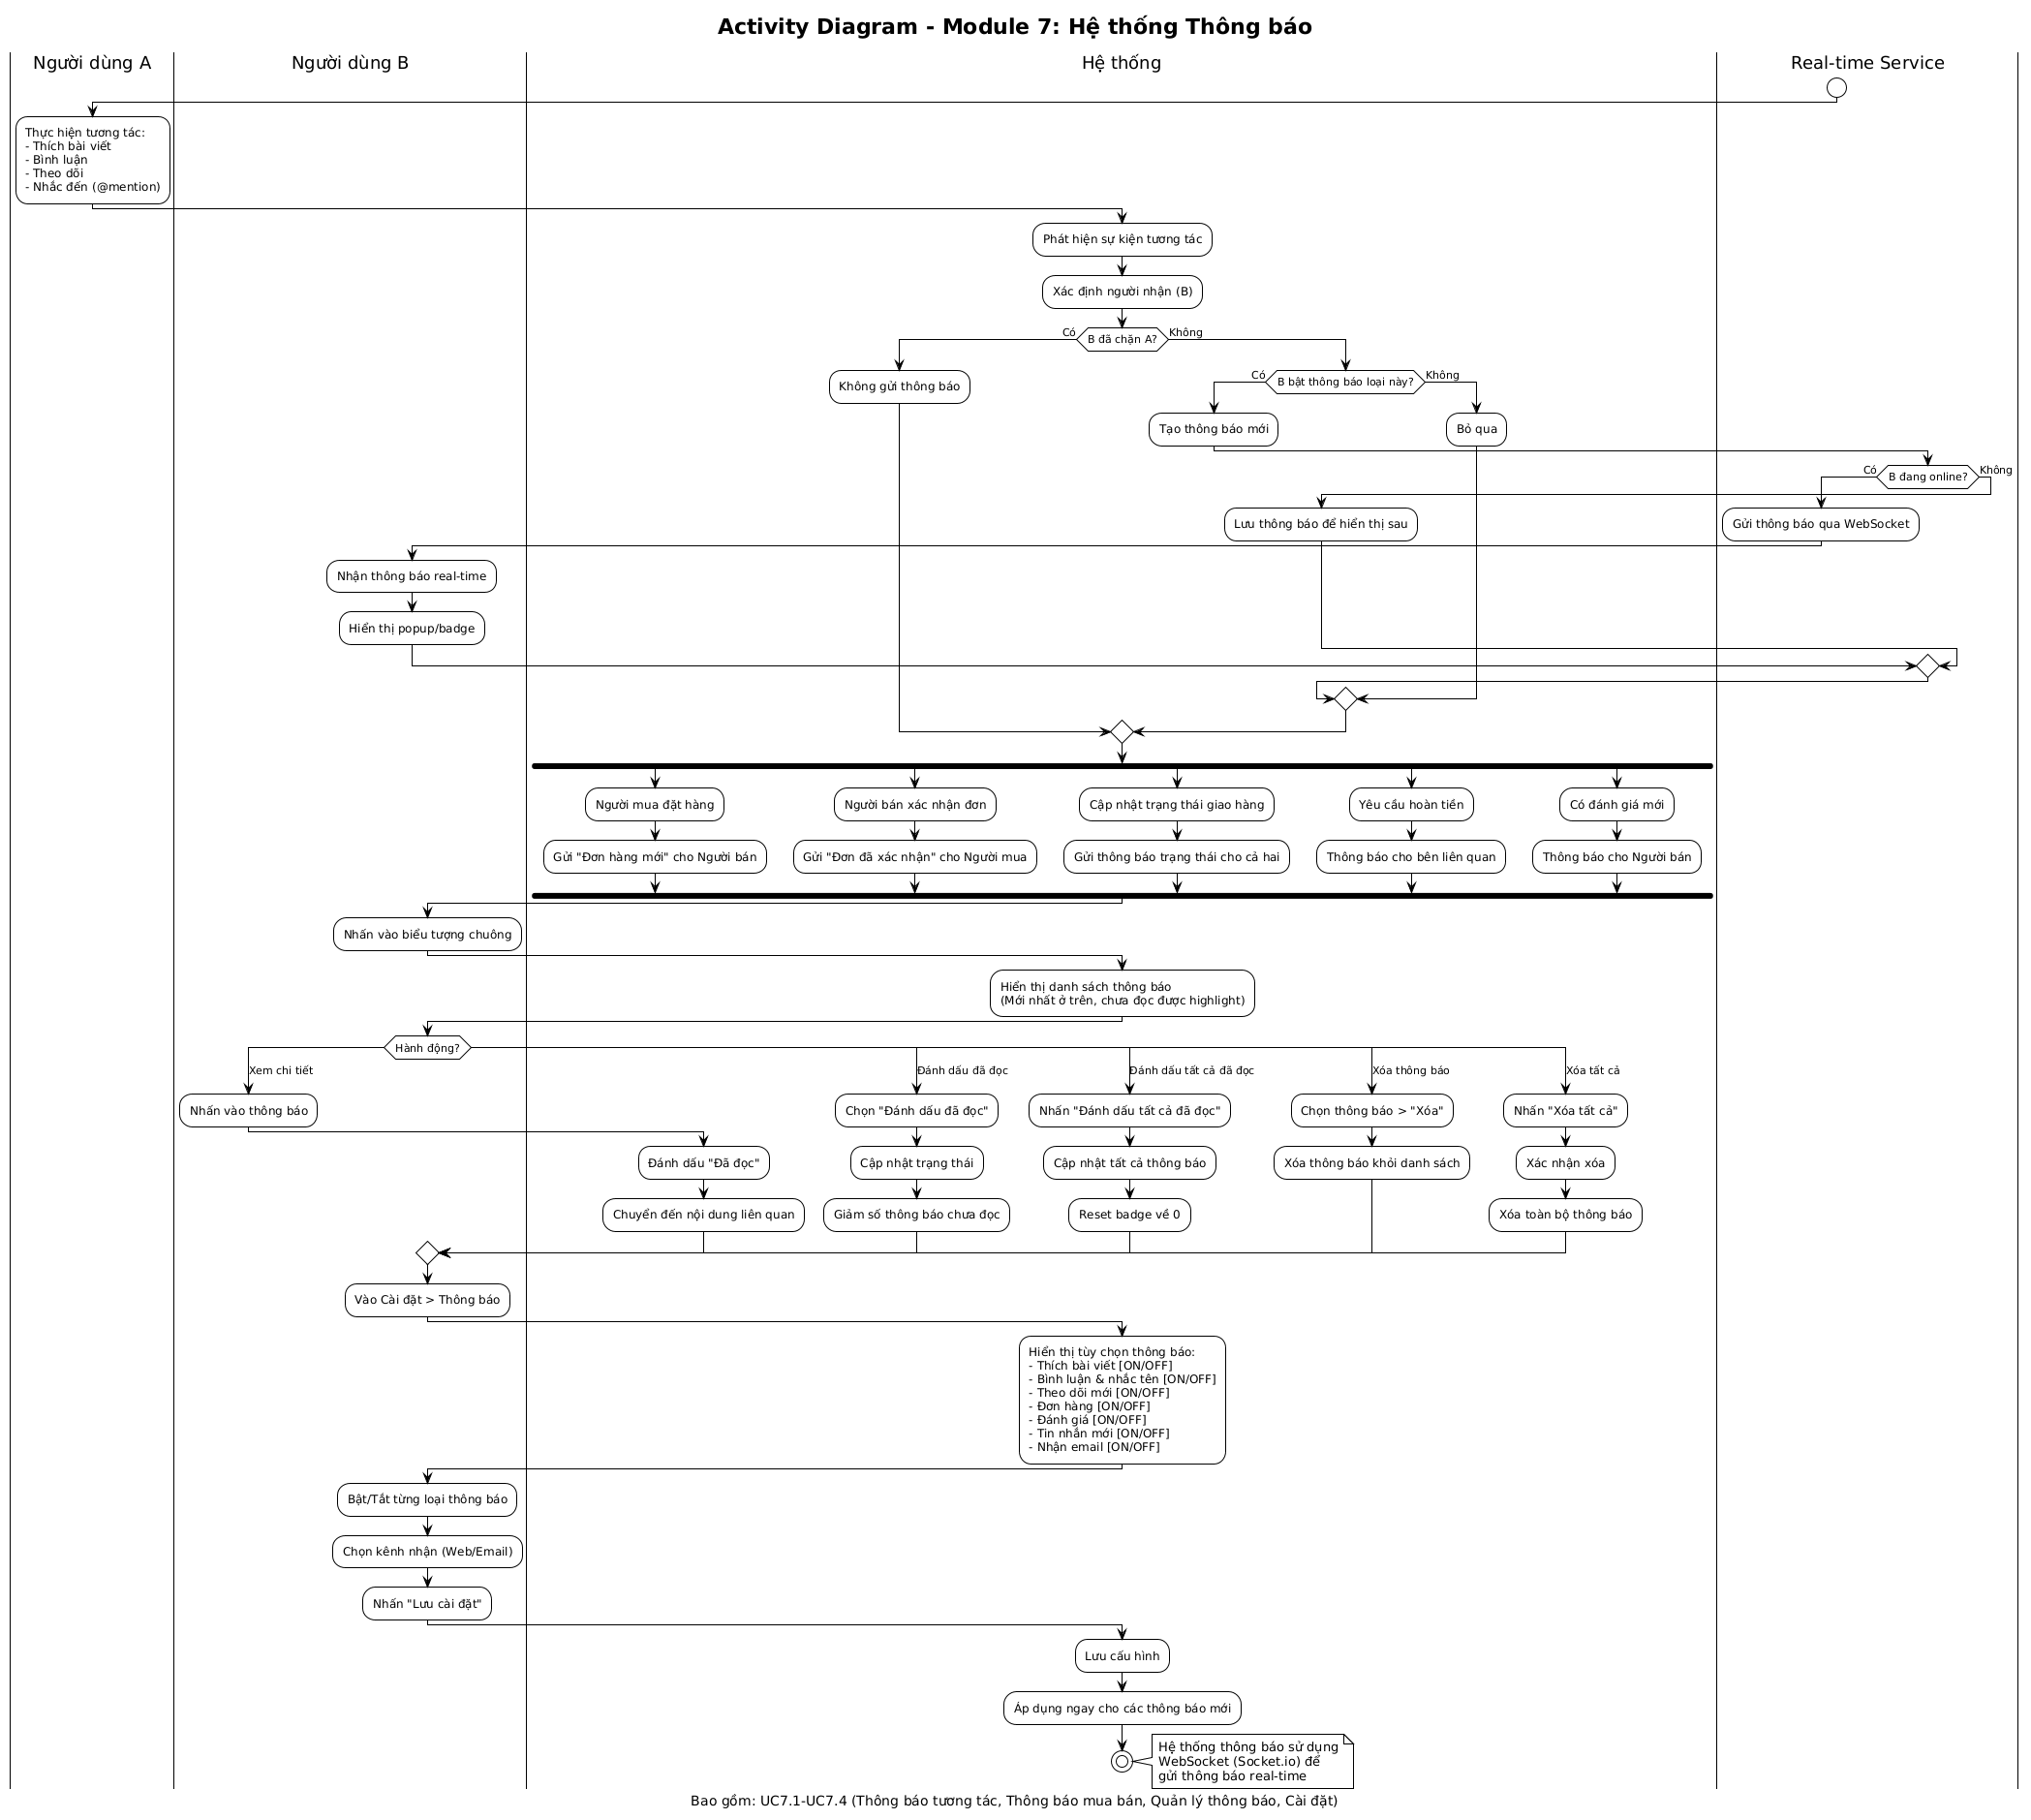
\includegraphics[width=\textwidth]{Images/Activity diagrams/AD-M7-NotificationSystem.png}
  \caption{Activity Diagram - Hệ thống Thông báo (AD-M7-NotificationSystem)}
\end{figure}


\section{Sequence diagram}
Phần này trình bày các Sequence Diagrams mô tả luồng tương tác giữa các thành phần hệ thống (Frontend, Controllers, Services, Database) thông qua các lời gọi API, kiểm tra điều kiện và phản hồi theo từng module. Mỗi module có mô tả tổng quan và các diagram chi tiết với hình ảnh minh họa.

\subsection{Module 1 – Quản lý Người dùng và Xác thực}

Module này mô tả luồng tương tác trong xác thực người dùng: đăng ký, đăng nhập với 2FA, khôi phục mật khẩu, quản lý hồ sơ, và nâng cấp lên Seller. Các diagram thể hiện cách Frontend giao tiếp với AuthController, UserController, EmailService và TokenService.

\subsubsection{SD-M1-Auth-RegisterLogin}

Diagram này mô tả chuỗi tương tác trong quá trình đăng ký và đăng nhập, bao gồm ba use case chính.

\textbf{UC1.1 – Đăng ký tài khoản:} Frontend gửi POST \texttt{/api/auth/register} với dữ liệu đăng ký. AuthController kiểm tra email đã tồn tại trong DB chưa. Nếu đã tồn tại, trả về 409 (Conflict). Nếu hợp lệ, AuthController tạo tài khoản với trạng thái \textit{unverified} và vai trò \textit{buyer}, gọi EmailService gửi email xác thực, và trả về 201 (Created).

\textbf{UC1.2 – Đăng nhập:} Frontend gửi POST \texttt{/api/auth/login} với email và mật khẩu. AuthController xác thực thông tin trong DB. Nếu sai/khóa/chưa xác thực, trả về 401/403. Nếu đúng và không bật 2FA, AuthController gọi TokenService tạo JWT, trả về 200 kèm token. Nếu bật 2FA, chuyển sang UC1.3.

\textbf{UC1.3 – Xác thực hai yếu tố (2FA):} AuthController gọi EmailService gửi mã OTP. Người dùng nhập mã OTP, Frontend gửi POST \texttt{/api/auth/verify-2fa}. AuthController kiểm tra mã OTP trong DB. Nếu hợp lệ, tạo JWT và trả về 200. Nếu sai/hết hạn, trả về 401.

\begin{figure}[H]
  \centering
  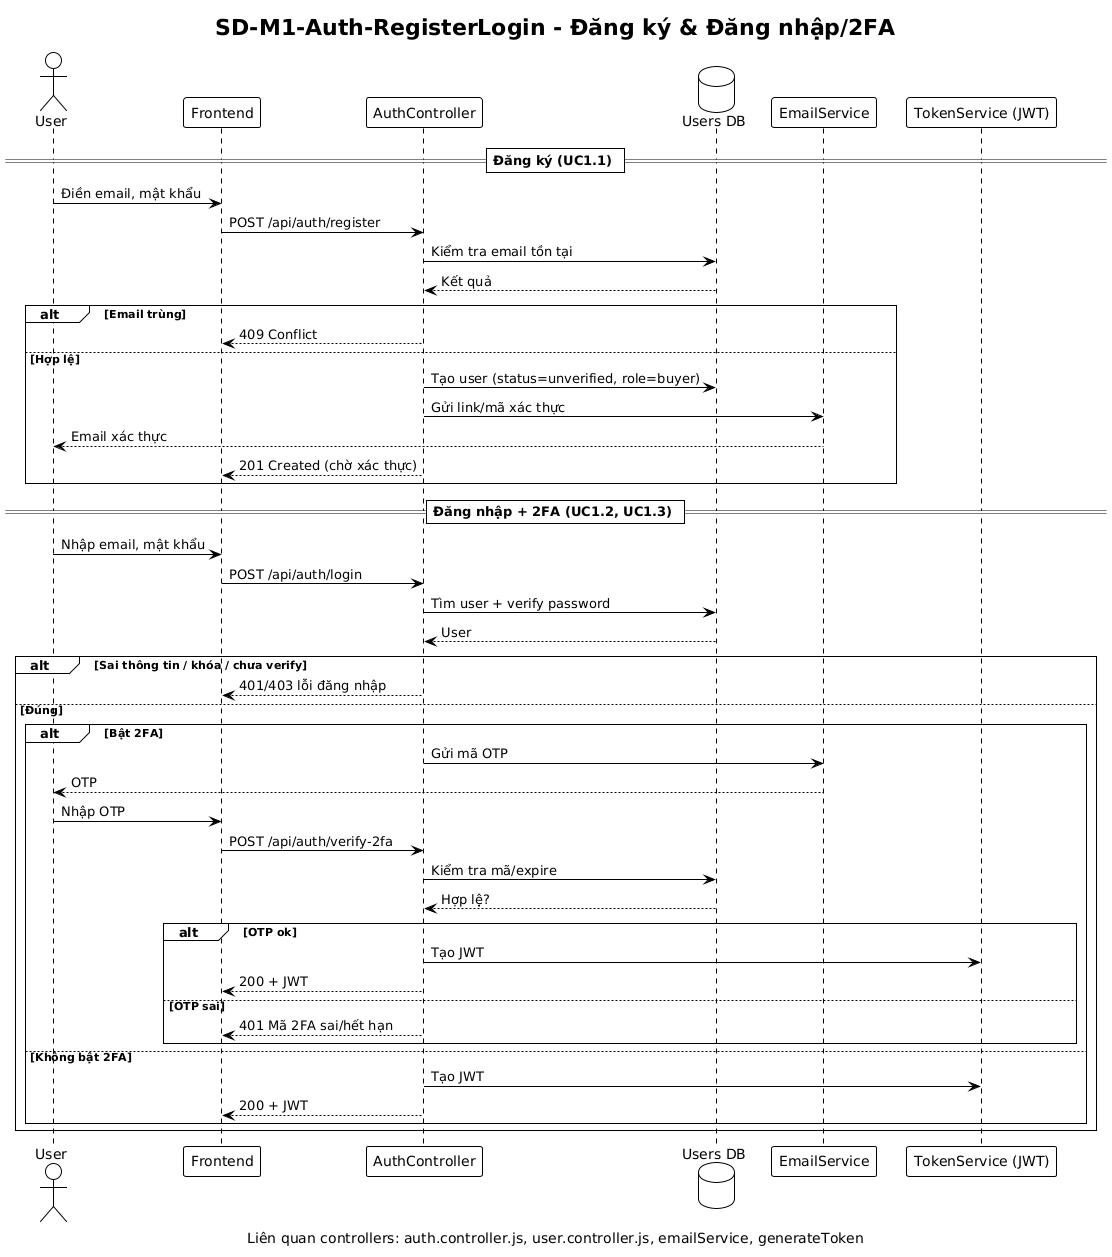
\includegraphics[width=\textwidth]{Images/Sequence diagrams/SD-M1-Auth-RegisterLogin.png}
  \caption{Sequence Diagram - Đăng ký và Đăng nhập (SD-M1-Auth-RegisterLogin)}
\end{figure}

\subsubsection{SD-M1-Auth-RecoveryLogout}

Diagram này mô tả chuỗi tương tác trong quá trình khôi phục mật khẩu và đăng xuất.

\textbf{UC1.4 – Khôi phục mật khẩu:} Frontend gửi POST \texttt{/api/auth/forgot-password} với email. AuthController xử lý yêu cầu theo cơ chế trả thông báo chung để tránh lộ thông tin tài khoản. Nếu email tồn tại, hệ thống tạo token reset, lưu vào DB và gọi EmailService gửi email. Người dùng mở link và đặt mật khẩu mới. Frontend gửi POST \texttt{/api/auth/reset-password} với token và mật khẩu mới. AuthController xác thực, hash mật khẩu và cập nhật trong DB, trả về 200.

\textbf{UC1.5 – Đăng xuất:} Frontend gửi POST \texttt{/api/auth/logout}. AuthController trả về kết quả đăng xuất, sau đó Frontend xóa token khỏi local storage và chuyển hướng về Trang chủ.

\begin{figure}[H]
  \centering
  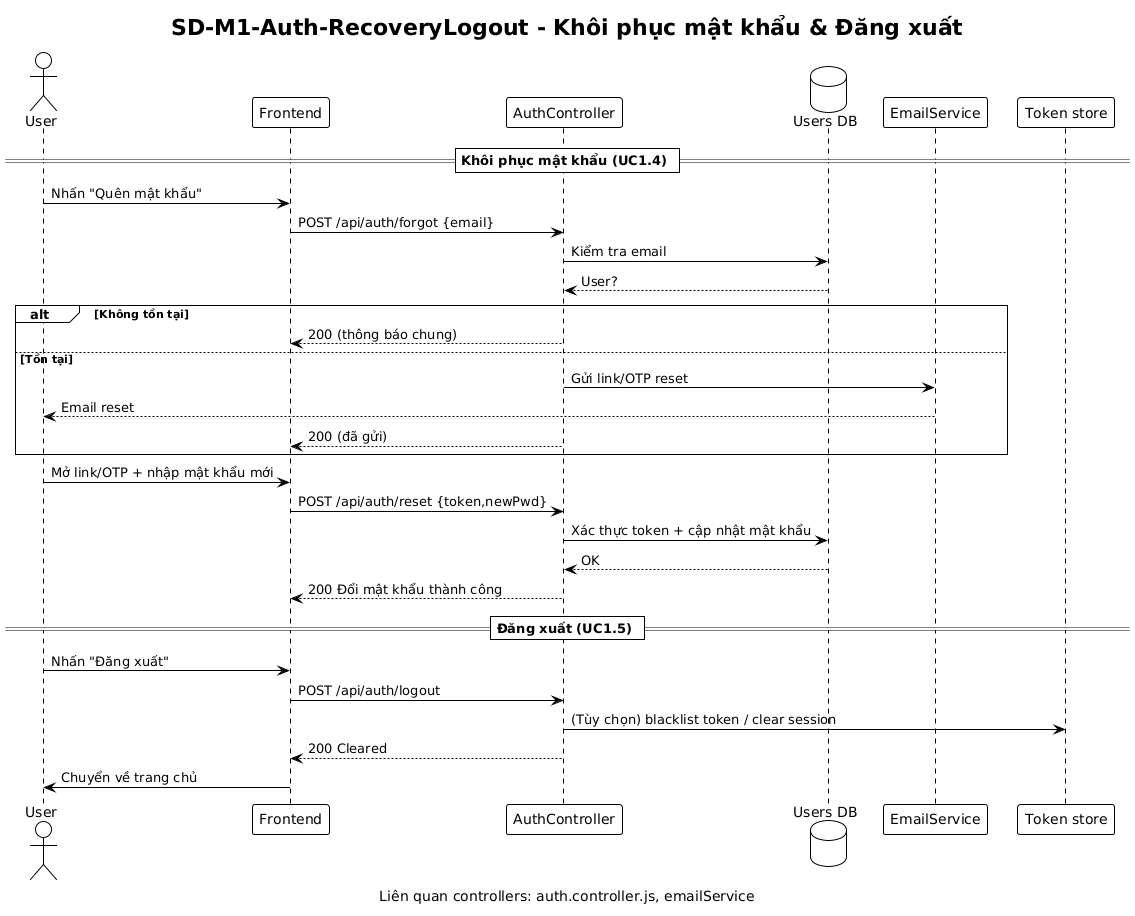
\includegraphics[width=\textwidth]{Images/Sequence diagrams/SD-M1-Auth-RecoveryLogout.png}
  \caption{Sequence Diagram - Khôi phục mật khẩu và Đăng xuất (SD-M1-Auth-RecoveryLogout)}
\end{figure}

\subsubsection{SD-M1-Profile-EditPrivacy}

Diagram này mô tả chuỗi tương tác trong quá trình chỉnh sửa hồ sơ và cài đặt quyền riêng tư.

\textbf{UC1.6 – Chỉnh sửa hồ sơ:} Frontend gửi PUT \texttt{/api/users/me} kèm dữ liệu cập nhật, file ảnh (nếu có) và JWT token. UserController xác thực token, nếu có ảnh thì gọi Storage service upload và nhận URL ảnh. UserController cập nhật thông tin trong Users DB, trả về 200 kèm hồ sơ mới.

\textbf{UC1.7 – Quyền riêng tư:} Frontend gửi PUT \texttt{/api/auth/privacy} kèm cấu hình quyền riêng tư và JWT token. AuthController xác thực token, lưu cấu hình vào Users DB và trả về 200.

\begin{figure}[H]
  \centering
  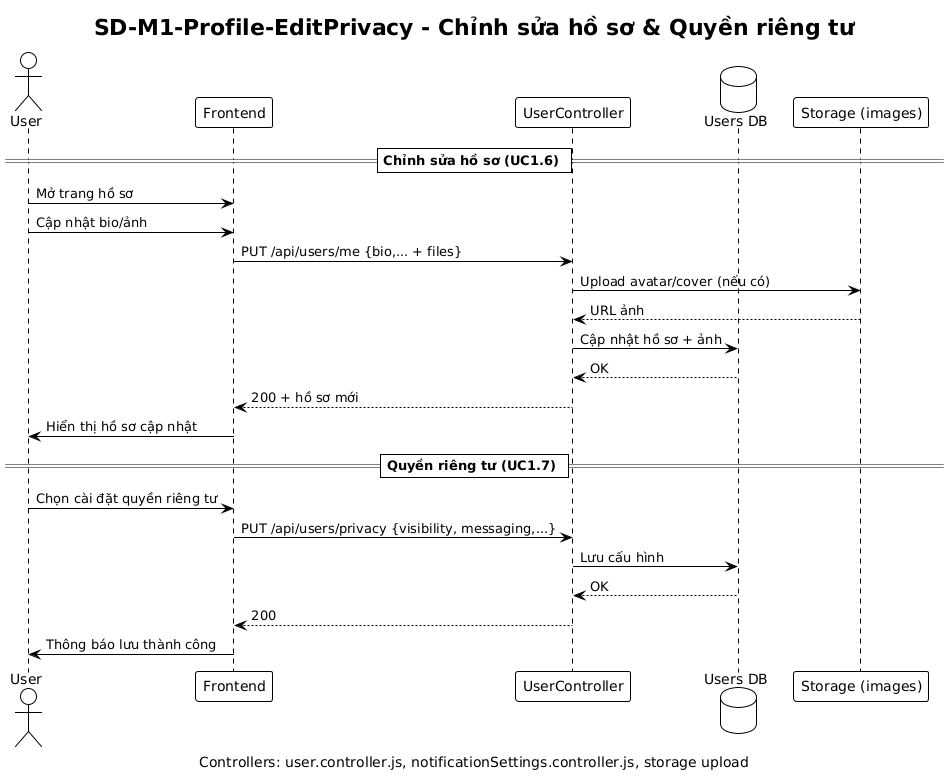
\includegraphics[width=\textwidth]{Images/Sequence diagrams/SD-M1-Profile-EditPrivacy.png}
  \caption{Sequence Diagram - Chỉnh sửa hồ sơ và Quyền riêng tư (SD-M1-Profile-EditPrivacy)}
\end{figure}

\subsubsection{SD-M1-Profile-SellerUpgrade}

Diagram này mô tả chuỗi tương tác trong quá trình đăng ký trở thành người bán.

\textbf{UC1.8 – Đăng ký Người bán:} Frontend gửi POST \texttt{/api/seller/apply} để khởi tạo hồ sơ, sau đó gửi dữ liệu qua các endpoint nhiều bước như \texttt{/api/seller/step1}, \texttt{/api/seller/step2}, \texttt{/api/seller/step3} hoặc \texttt{/api/seller/register-with-uploads}. SellerController xác thực, lưu hồ sơ vào bảng \textit{seller\_verifications} và chuyển trạng thái sang chờ duyệt. Admin xử lý qua admin API; nếu duyệt, hệ thống cập nhật role của user thành \textit{SELLER}.

\begin{figure}[H]
  \centering
  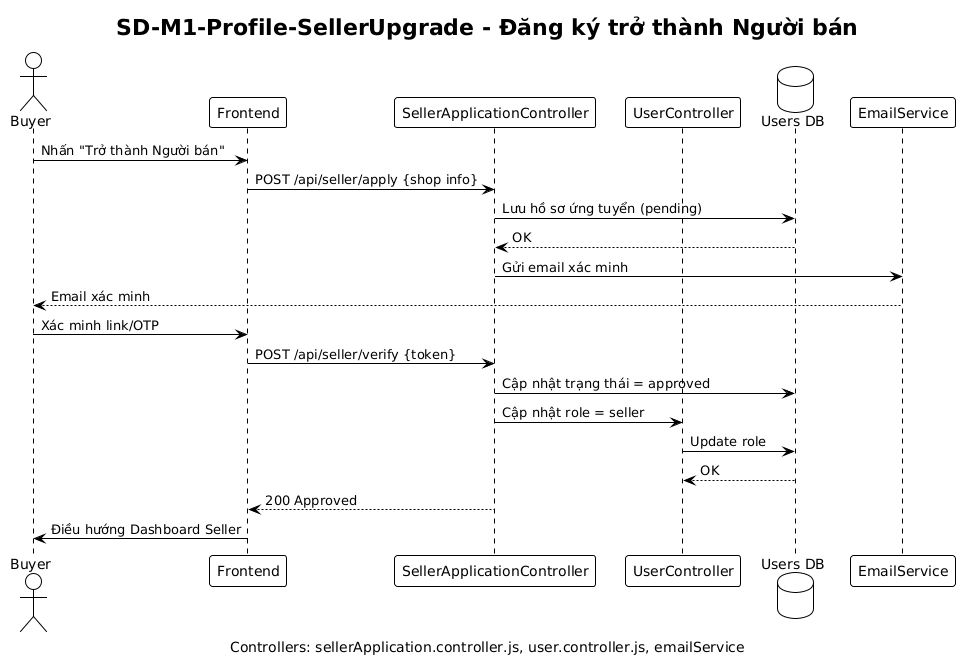
\includegraphics[width=\textwidth]{Images/Sequence diagrams/SD-M1-Profile-SellerUpgrade.png}
  \caption{Sequence Diagram - Đăng ký trở thành Người bán (SD-M1-Profile-SellerUpgrade)}
\end{figure}

\subsection{Module 2 – Tương tác Xã hội}

Module này mô tả luồng tương tác trong tính năng mạng xã hội: xem feed, tạo và tương tác với bài đăng, follow, nhắn tin, tham gia nhóm, báo cáo vi phạm. Các diagram thể hiện cách Frontend giao tiếp với PostController, UserController, MessageController, ReportController, FeedService, ProductController và NotificationService.

\subsubsection{SD-M2-FeedAndPosts}

Diagram này mô tả chuỗi tương tác trong quá trình xem feed, tạo bài đăng và tương tác với nội dung.

\textbf{UC2.1 – Xem Feed:} Frontend gửi GET \texttt{/api/posts/feed} kèm JWT token và tham số phân trang để lấy personalized feed, hoặc GET \texttt{/api/posts} cho feed công khai. PostController gọi PostService truy vấn DB lấy bài đăng từ người đang theo dõi kết hợp gợi ý, trả về danh sách đã sắp xếp. Frontend hiển thị với infinite scroll.

\textbf{UC2.2 và UC2.3 – Tạo bài đăng và gắn thẻ sản phẩm:} Nếu Seller muốn gắn sản phẩm, Frontend có thể lấy sản phẩm của seller qua các endpoint sản phẩm dành cho seller như \texttt{/api/products/seller/me}. Sau khi chọn một hoặc nhiều sản phẩm, Frontend gửi POST \texttt{/api/posts} kèm nội dung, media, mảng \texttt{productTags} và JWT token. PostController xác thực, kiểm tra nội dung, PostService lưu bài đăng vào \textit{posts} và lưu các tag vào \textit{post\_product\_tags}, sau đó trả về 201.

\textbf{UC2.4 – Tương tác với bài đăng:} Frontend gửi POST \texttt{/api/posts/:id/like} hoặc \texttt{/api/posts/:id/comments} kèm nội dung (nếu comment) và JWT token. PostController xác thực, lưu lượt thích/bình luận vào DB, gọi NotificationService gửi thông báo đến chủ sở hữu bài đăng, trả về 200 kèm trạng thái mới.

\begin{figure}[H]
  \centering
  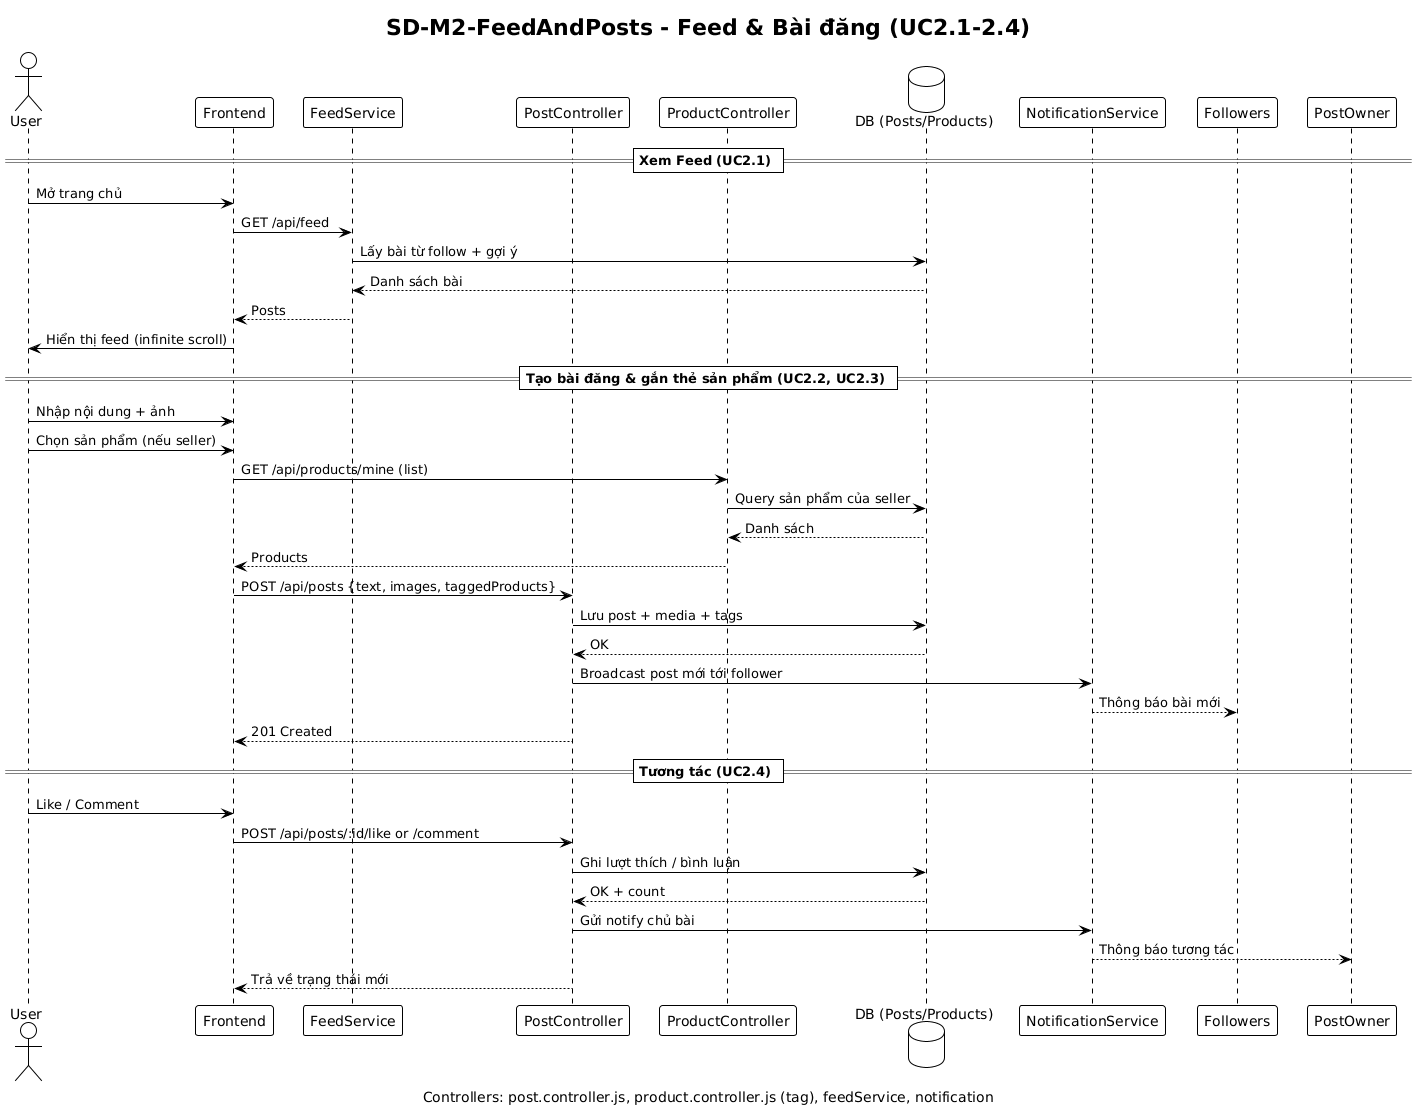
\includegraphics[width=\textwidth]{Images/Sequence diagrams/SD-M2-FeedAndPosts.png}
  \caption{Sequence Diagram - Feed và Bài đăng (SD-M2-FeedAndPosts)}
\end{figure}

\subsubsection{SD-M2-SocialConnections}

Diagram này mô tả chuỗi tương tác trong các kết nối xã hội giữa người dùng.

\textbf{UC2.5 – Theo dõi người dùng:} Frontend gửi POST \texttt{/api/users/:bId/follow} kèm JWT token. UserController xác thực, kiểm tra A chưa follow B, tạo mối quan hệ UserFollow trong DB, gọi NotificationService gửi thông báo đến B, trả về 200.

\textbf{UC2.6 – Nhắn tin 1-1:} Frontend gửi POST \texttt{/api/messages/conversations} để lấy hoặc tạo conversation với người nhận. Khi gửi tin nhắn, Frontend gửi POST \texttt{/api/messages/conversations/:conversationId} kèm nội dung và JWT token. MessageController xác thực người gửi thuộc conversation, lưu tin nhắn vào DB, emit realtime qua Socket.IO và tạo notification nếu người nhận offline.

\textbf{UC2.7 – Tham gia nhóm:} Frontend gửi POST \texttt{/api/groups/:groupId/join} kèm JWT token. GroupController xác thực, kiểm tra loại nhóm. Nếu công khai, thêm membership ngay; nếu riêng tư, tạo yêu cầu tham gia với trạng thái \textit{pending}. Lưu vào DB và trả về kết quả.

\textbf{UC2.8 – Báo cáo vi phạm:} Frontend gửi POST \texttt{/api/reports} kèm targetType, targetId, reason, description (nếu có) và JWT token. ReportController xác thực, lưu báo cáo với trạng thái \textit{pending} vào DB và trả về kết quả. Admin xem báo cáo qua admin API.

\begin{figure}[H]
  \centering
  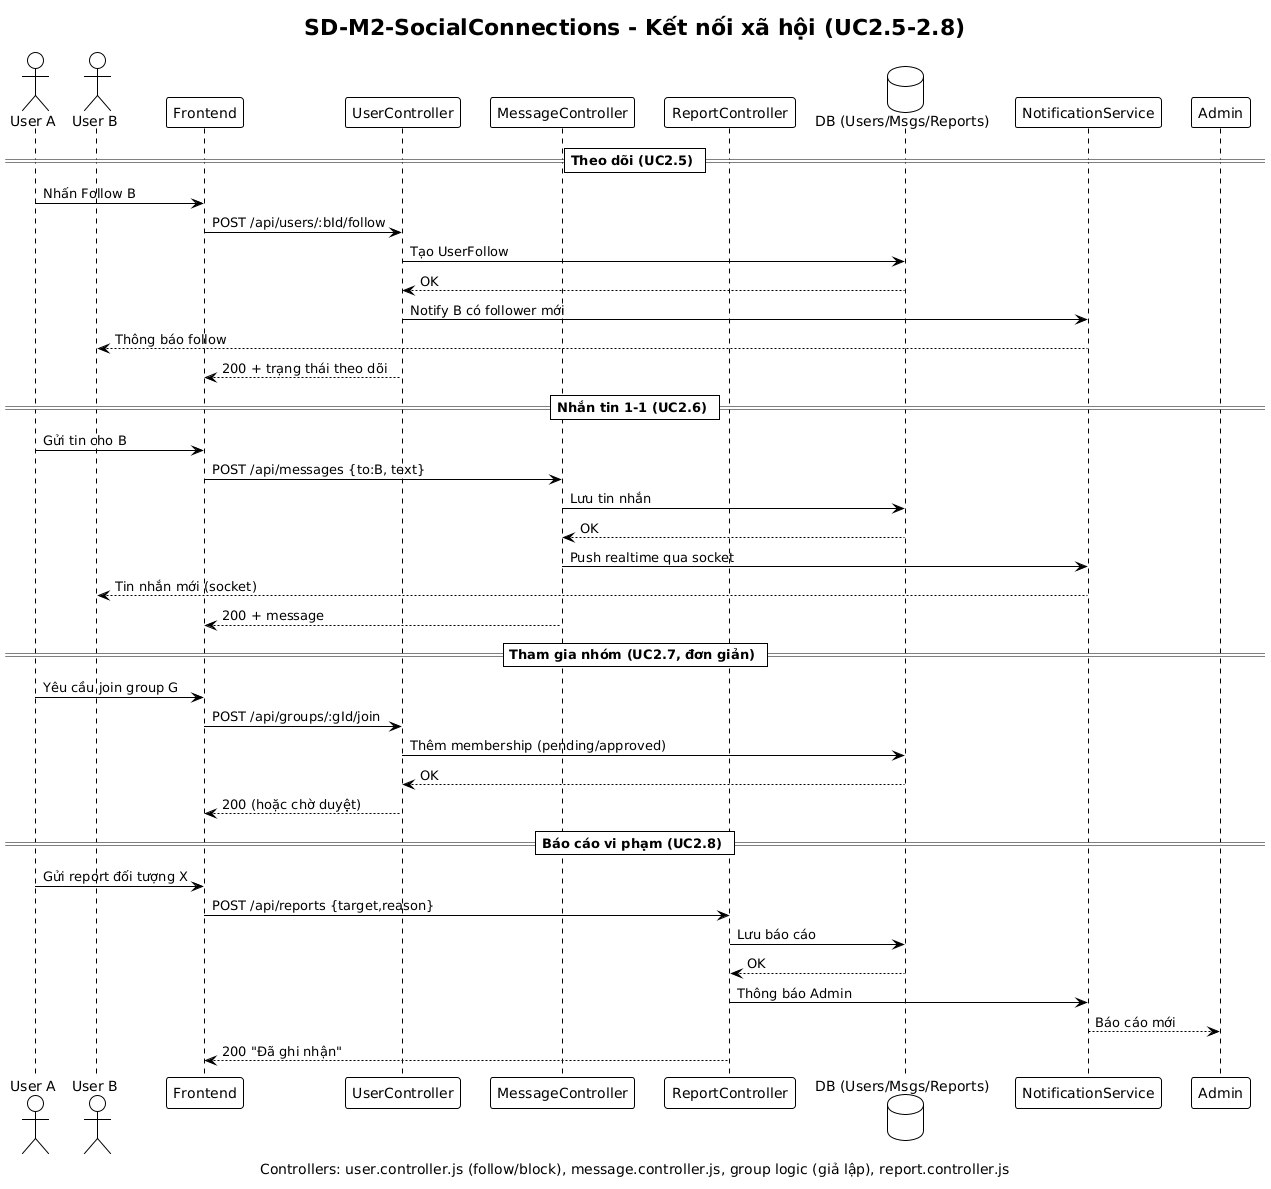
\includegraphics[width=\textwidth]{Images/Sequence diagrams/SD-M2-SocialConnections.png}
  \caption{Sequence Diagram - Kết nối Xã hội (SD-M2-SocialConnections)}
\end{figure}

\subsection{Module 3 – Hoạt động Thương mại}

Module này mô tả luồng tương tác trong hệ sinh thái thương mại: hành trình mua hàng của Buyer (tìm kiếm, xem sản phẩm, giỏ hàng, thanh toán, theo dõi đơn hàng, đánh giá) và tác vụ của Seller (quản lý sản phẩm, xử lý đơn hàng, hoàn tiền, phản hồi đánh giá). Các diagram thể hiện cách Frontend giao tiếp với ProductController, CartController, OrderController, ReviewController và NotificationService.

\subsubsection{SD-M3-BuyerFlow}

Diagram này mô tả chuỗi tương tác trong toàn bộ quy trình mua hàng từ góc nhìn của Buyer.

\textbf{UC3.1 và UC3.2 – Tìm kiếm và xem sản phẩm:} Frontend gửi GET \texttt{/api/products?query=...\&filters=...} với tham số tìm kiếm và lọc. ProductController truy vấn DB, trả về danh sách sản phẩm. Frontend hiển thị danh sách. Để xem chi tiết, Frontend gửi GET \texttt{/api/products/:id}. ProductController truy vấn DB lấy chi tiết và biến thể, trả về dữ liệu chi tiết.

\textbf{UC3.3 và UC3.4 – Quản lý giỏ hàng:} Frontend gửi POST \texttt{/api/cart/items} kèm ID sản phẩm, biến thể, số lượng và JWT token. CartController xác thực, kiểm tra tồn kho, lưu cart item vào DB, trả về giỏ hàng đã cập nhật. Để cập nhật/xóa: Frontend gửi PATCH \texttt{/api/cart/items/:id} hoặc DELETE. CartController cập nhật/xóa trong DB, tính lại tổng tiền, trả về giỏ hàng đã cập nhật.

\textbf{UC3.5 – Thanh toán:} Frontend gửi POST \texttt{/api/orders} kèm thông tin giỏ hàng, địa chỉ giao hàng, phương thức thanh toán và JWT token. OrderController xác thực, kiểm tra tồn kho. Nếu đủ hàng, tạo Order với trạng thái \textit{Processing} và OrderItems trong DB, gọi NotificationService gửi thông báo đến Seller, trả về 201. Nếu hết hàng, trả về 400.

\textbf{UC3.6 và UC3.7 – Theo dõi đơn hàng và đánh giá:} Frontend gửi GET \texttt{/api/orders/my/purchases} kèm JWT token. OrderController xác thực, truy vấn DB lấy danh sách đơn hàng của Buyer, trả về danh sách. Khi đơn hàng đã giao hoặc hoàn thành, Frontend gửi POST \texttt{/api/reviews} kèm ID order item, số sao, nhận xét, hình ảnh (nếu có) và JWT token. ReviewController xác thực, lưu đánh giá vào DB, trả về 201.

\begin{figure}[H]
  \centering
  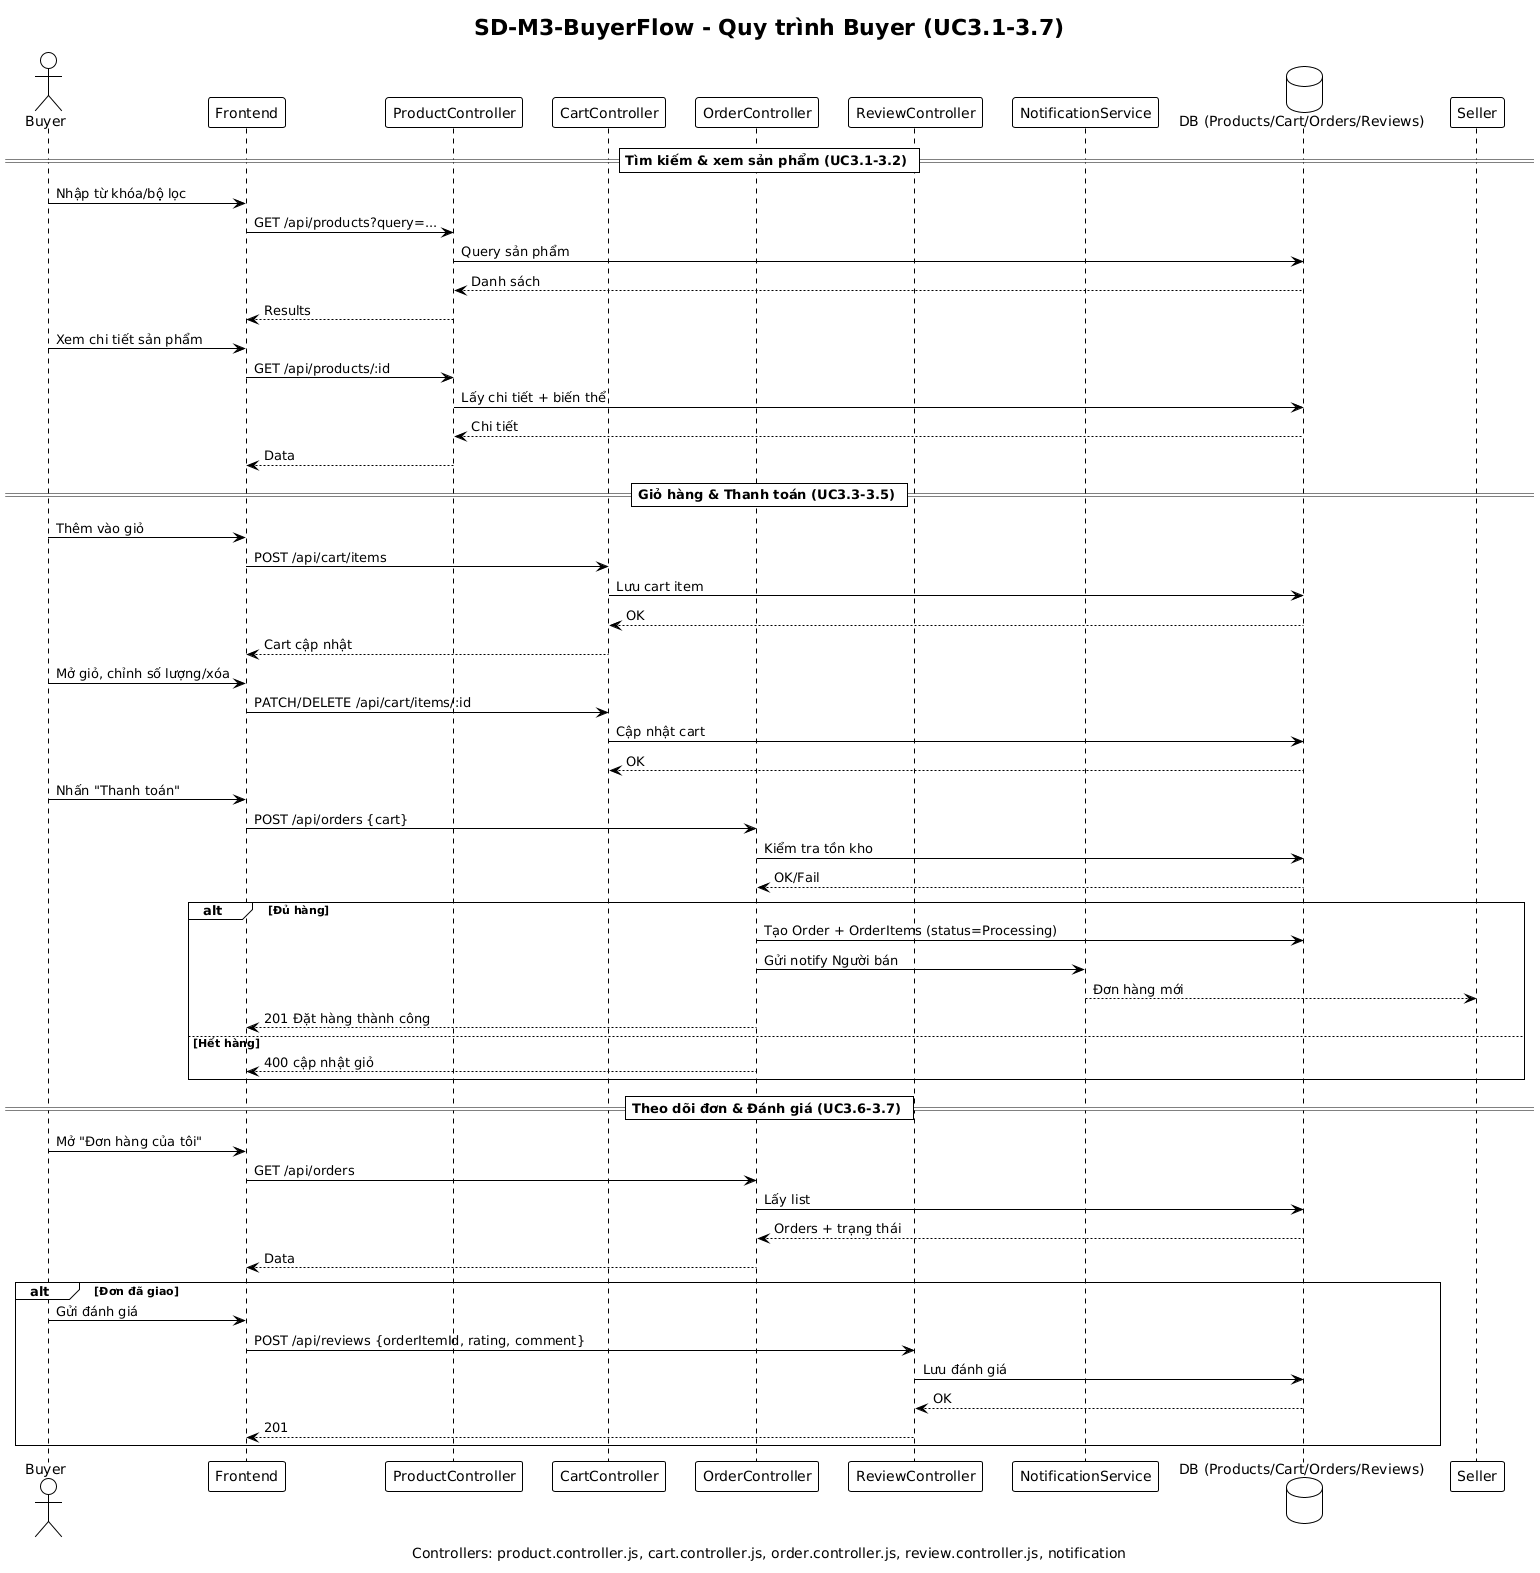
\includegraphics[width=\textwidth]{Images/Sequence diagrams/SD-M3-BuyerFlow.png}
  \caption{Sequence Diagram - Quy trình Mua hàng (SD-M3-BuyerFlow)}
\end{figure}

\subsubsection{SD-M3-Seller-ProductsOrders}

Diagram này mô tả chuỗi tương tác trong quá trình quản lý sản phẩm và đơn hàng của Seller.

\textbf{UC3.8 – Quản lý sản phẩm:} Frontend gửi POST \texttt{/api/products} (thêm), PUT \texttt{/api/products/:id} (sửa), hoặc DELETE \texttt{/api/products/:id} (xóa) kèm dữ liệu sản phẩm và JWT token. ProductController xác thực token và vai trò Seller, thực hiện lưu/cập nhật/soft-delete sản phẩm cùng biến thể trong DB, trả về 200/201.

\textbf{UC3.10 – Quản lý đơn hàng:} Frontend gửi GET \texttt{/api/orders/my/sales} kèm JWT token. OrderController xác thực token và vai trò Seller, truy vấn DB lấy danh sách đơn hàng của shop, trả về danh sách. Để cập nhật trạng thái: Frontend gửi PUT \texttt{/api/orders/:orderId/status} kèm trạng thái mới và JWT token. OrderController xác thực quyền, cập nhật trạng thái trong DB, gọi NotificationService thông báo Buyer, trả về 200.

\begin{figure}[H]
  \centering
  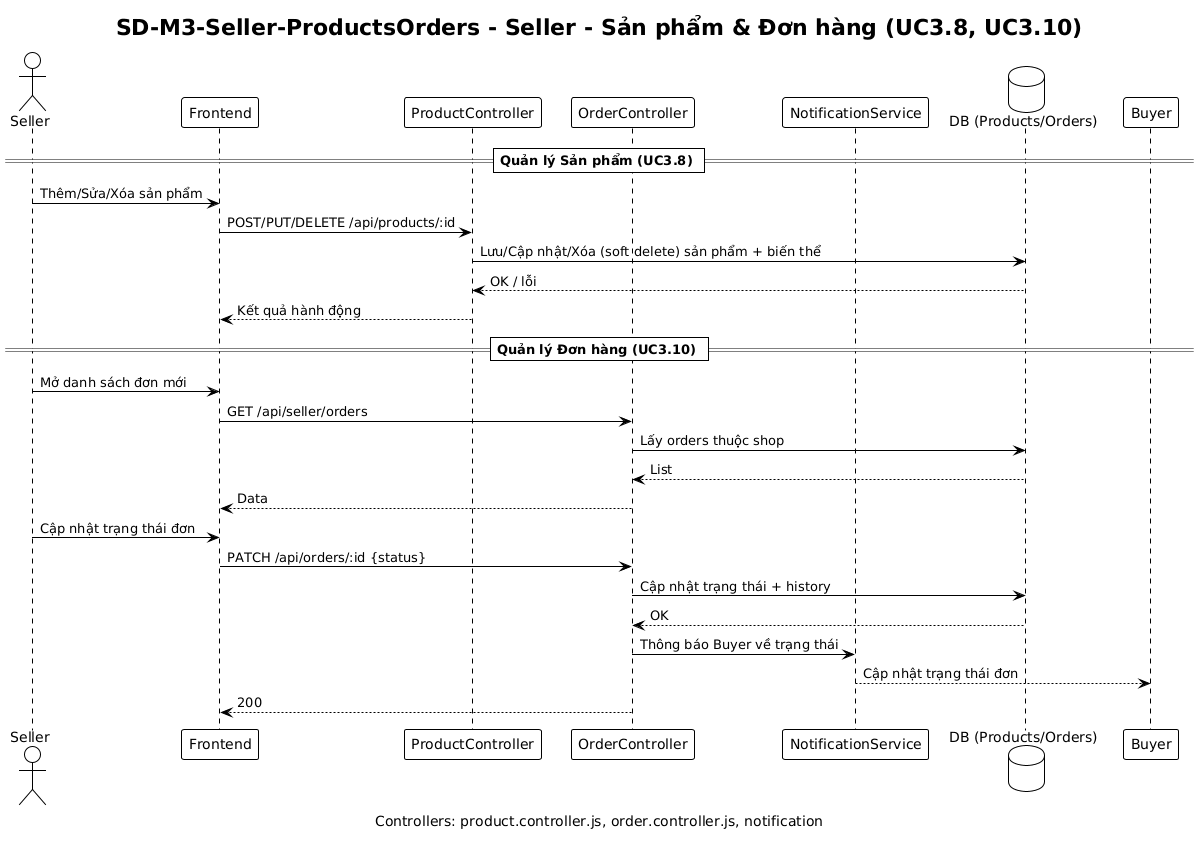
\includegraphics[width=\textwidth]{Images/Sequence diagrams/SD-M3-Seller-ProductsOrders.png}
  \caption{Sequence Diagram - Quản lý Sản phẩm và Đơn hàng của Seller (SD-M3-Seller-ProductsOrders)}
\end{figure}

\subsubsection{SD-M3-Seller-RefundReview}

Diagram này mô tả chuỗi tương tác trong quá trình xử lý hoàn tiền và phản hồi đánh giá của Seller.

\textbf{UC3.11 – Xử lý hoàn tiền:} Frontend gửi GET \texttt{/api/orders/seller/refunds} kèm JWT token. OrderController xác thực, truy vấn DB lấy danh sách yêu cầu hoàn tiền, trả về danh sách. Seller quyết định: Frontend gửi POST \texttt{/api/orders/:orderId/refund} kèm quyết định và lý do. OrderController cập nhật trạng thái/lý do liên quan trong phạm vi giả lập, gọi NotificationService thông báo Buyer và trả về kết quả.

\textbf{UC3.12 – Phản hồi đánh giá:} Frontend gửi POST \texttt{/api/reviews/:id/reply} kèm nội dung phản hồi và JWT token. ReviewController xác thực token và vai trò Seller, lưu phản hồi vào DB, gọi NotificationService thông báo Buyer, trả về 201.

\begin{figure}[H]
  \centering
  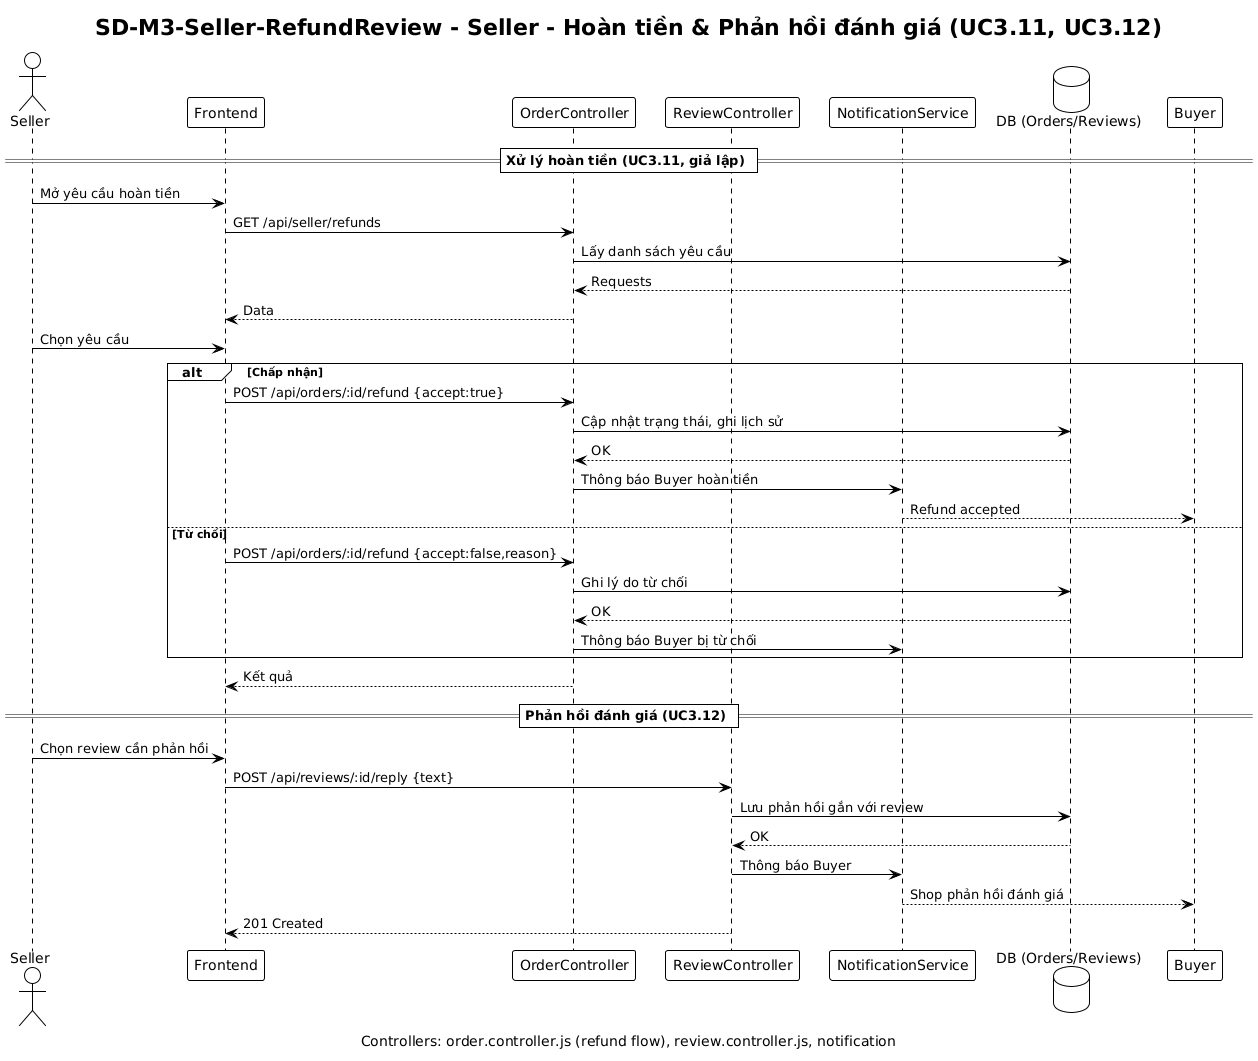
\includegraphics[width=\textwidth]{Images/Sequence diagrams/SD-M3-Seller-RefundReview.png}
  \caption{Sequence Diagram - Hoàn tiền và Phản hồi Đánh giá của Seller (SD-M3-Seller-RefundReview)}
\end{figure}

\subsection{Module 4 – Hệ thống Quản trị}

Module này mô tả luồng tương tác trong công cụ quản trị: quản lý tài khoản, quản lý nội dung, xử lý báo cáo vi phạm, và thống kê phân tích. Các diagram thể hiện cách Frontend giao tiếp với Admin Controllers (UsersController, PostsController, ProductsController, ReportsController, DashboardController) và Database.

\subsubsection{SD-M4-Admin-AccountsContent}

Diagram này mô tả chuỗi tương tác trong quá trình quản lý tài khoản và nội dung của Admin.

\textbf{UC4.1 – Quản lý tài khoản:} Admin Frontend gửi GET \texttt{/api/admin/users?filters=...} đến admin API với tham số lọc và admin JWT. AdminController xác thực token và vai trò Admin, truy vấn DB, trả về danh sách người dùng. Để thực hiện hành động: Frontend gửi PATCH \texttt{/api/admin/users/:id/toggle-active} hoặc PATCH \texttt{/api/admin/users/:id/role}. Controller xác thực quyền, cập nhật trong DB, trả về 200.

\textbf{UC4.2 – Quản lý nội dung:} Admin Frontend gửi GET \texttt{/api/admin/posts} hoặc \texttt{/api/admin/products} kèm admin JWT. AdminController xác thực token và vai trò Admin, truy vấn DB, trả về danh sách. Để xóa: Frontend gửi DELETE \texttt{/api/admin/posts/:id} hoặc \texttt{/api/admin/products/:id}. Controller xác thực quyền, xóa nội dung trong DB và trả về 200.

\begin{figure}[H]
  \centering
  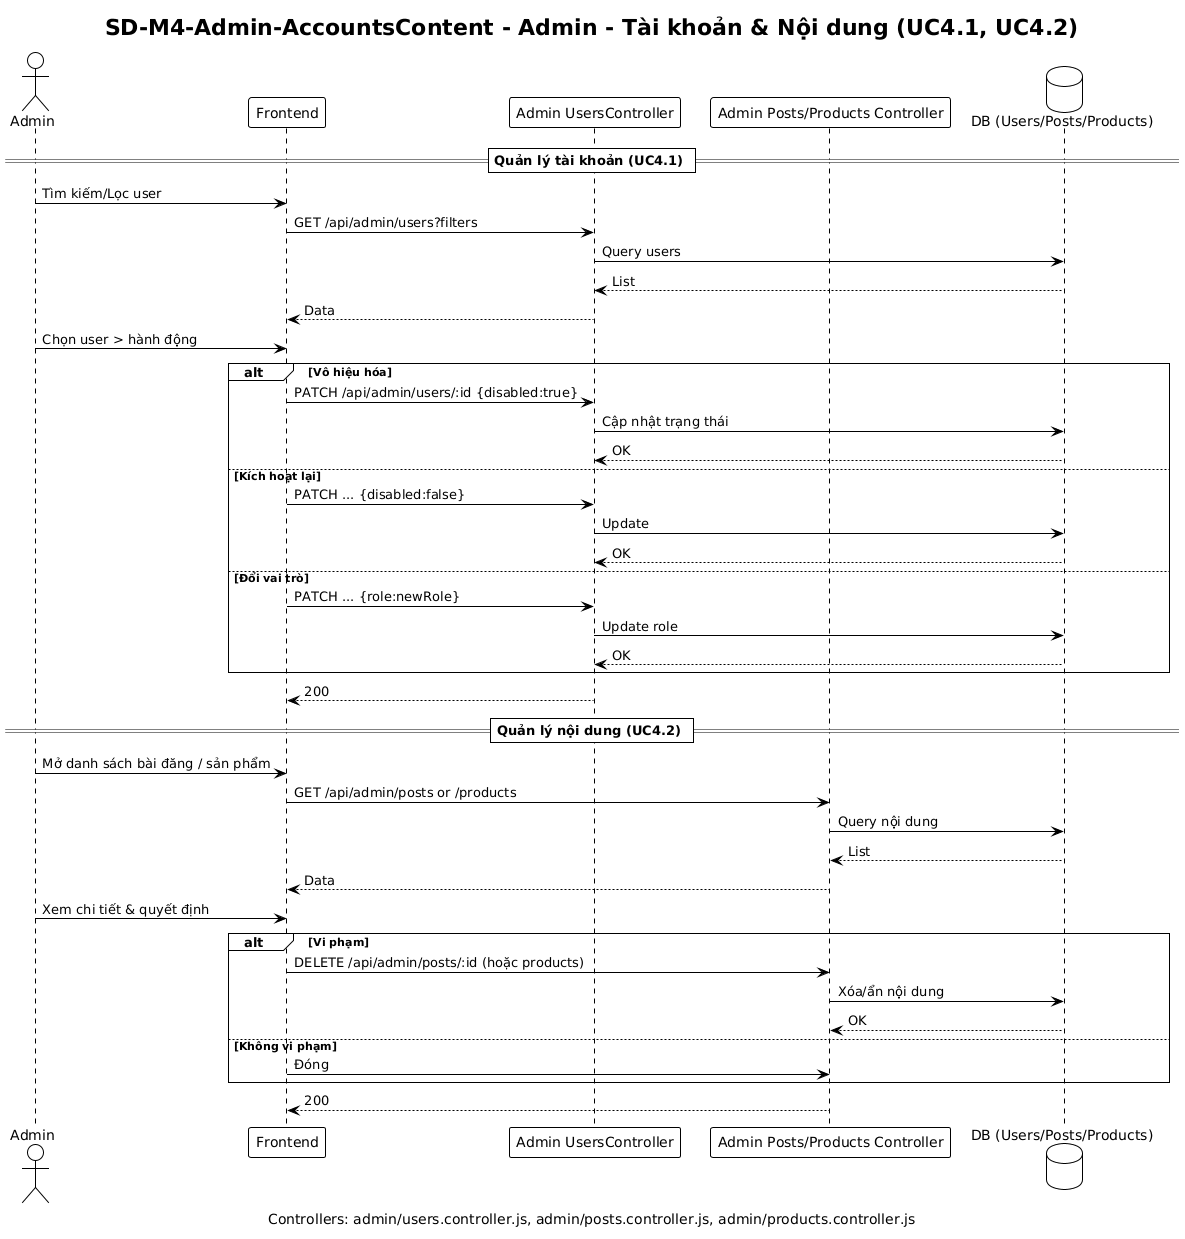
\includegraphics[width=\textwidth]{Images/Sequence diagrams/SD-M4-Admin-AccountsContent.png}
  \caption{Sequence Diagram - Quản lý Tài khoản và Nội dung của Admin (SD-M4-Admin-AccountsContent)}
\end{figure}

\subsubsection{SD-M4-Admin-ReportsAnalytics}

Diagram này mô tả chuỗi tương tác trong quá trình xử lý báo cáo và xem thống kê của Admin.

\textbf{UC4.3 – Xử lý báo cáo vi phạm:} Admin Frontend gửi GET \texttt{/api/reports?status=pending} đến admin API kèm admin JWT. ReportController xác thực, truy vấn DB lấy danh sách báo cáo pending, trả về danh sách. Để xem chi tiết: Frontend gửi GET \texttt{/api/reports/:reportId}. Để xử lý: Frontend gửi PATCH \texttt{/api/reports/:reportId/resolve} kèm action và admin JWT. Controller xác thực quyền, thực thi hành động trong DB, trả về 200.

\textbf{UC4.4 – Thống kê và phân tích:} Admin Frontend gửi GET \texttt{/api/admin/dashboard} hoặc \texttt{/api/admin/dashboard/growth?days=...} kèm admin JWT. AdminController xác thực, truy vấn DB tổng hợp số liệu về người dùng, bài đăng, sản phẩm, đơn hàng, doanh thu và growth, trả về dữ liệu thống kê.

\begin{figure}[H]
  \centering
  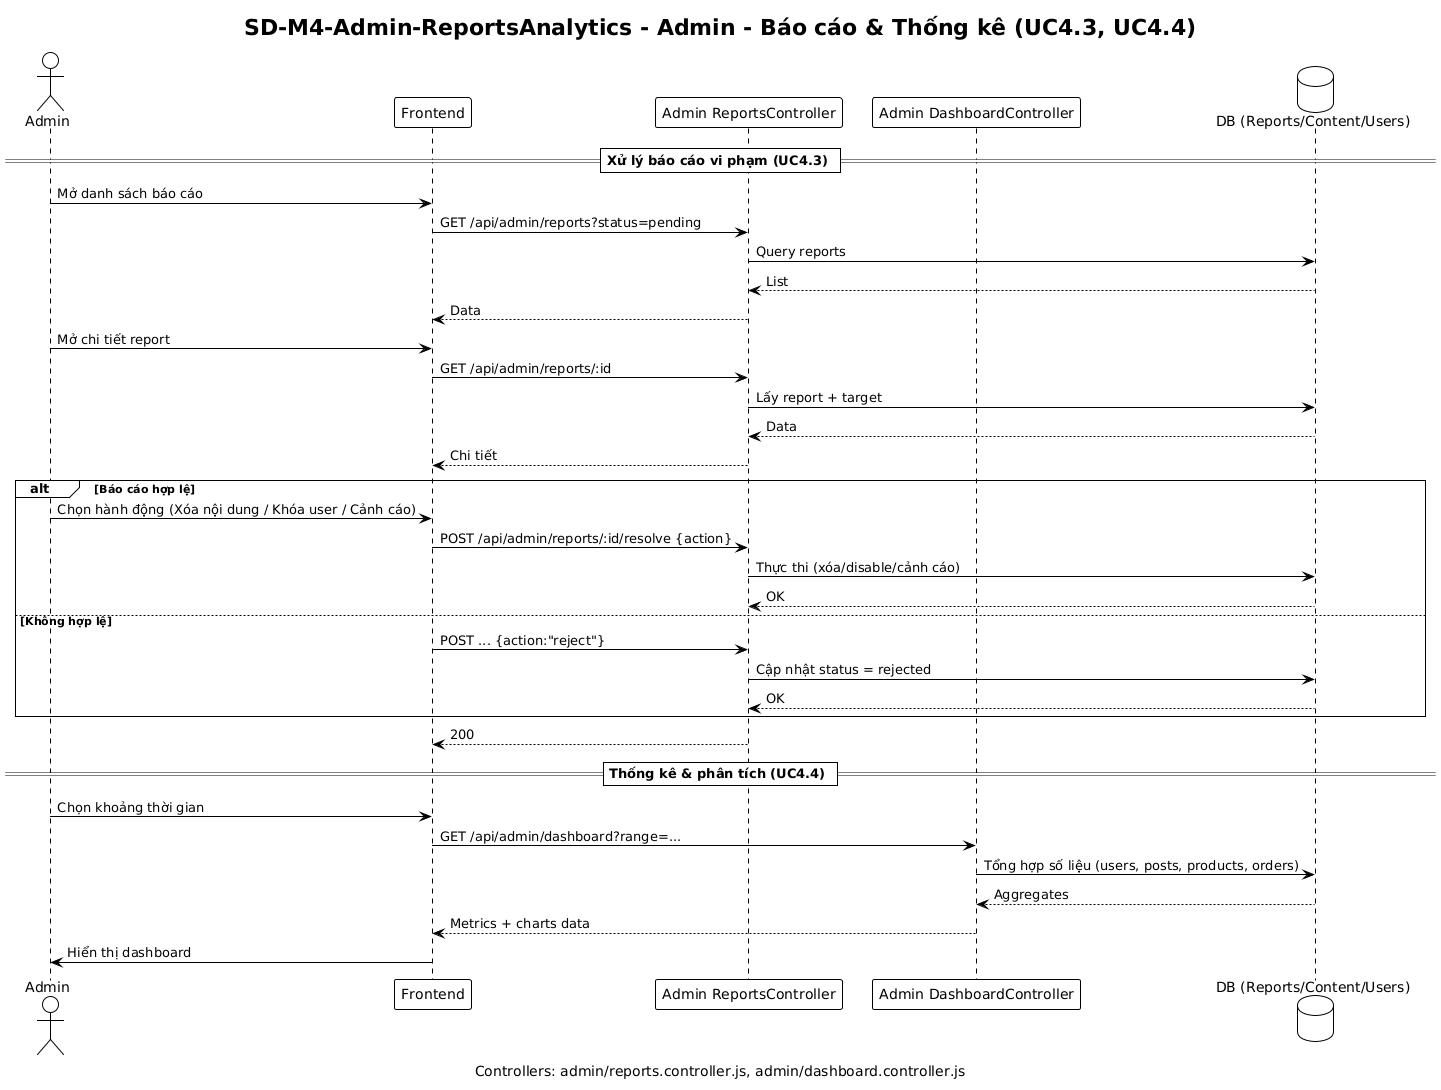
\includegraphics[width=\textwidth]{Images/Sequence diagrams/SD-M4-Admin-ReportsAnalytics.png}
  \caption{Sequence Diagram - Báo cáo và Thống kê của Admin (SD-M4-Admin-ReportsAnalytics)}
\end{figure}

\subsection{Module 5 – Tích hợp AI hỗ trợ}

Module này mô tả luồng tương tác trong tính năng AI hỗ trợ tạo nội dung và AI Shopping Assistant: generate text, generate image+text, quản lý lịch sử nội dung AI và chatbox tư vấn mua sắm. Các diagram thể hiện cách Frontend giao tiếp với AIController, AI Assistant Controller, AI Service, external AI providers và Database.

\subsubsection{SD-M5-AIContentCreation}

Diagram này mô tả chuỗi tương tác trong quá trình tạo nội dung sử dụng AI và tư vấn mua sắm qua chatbox.

\textbf{UC5.1 – Generate Text:} Frontend gửi POST \texttt{/api/ai/generate-text} kèm mô tả, ý tưởng, hình ảnh (nếu có) và JWT token. AIController xác thực, gọi AI Service. AI Service chuẩn hóa đầu vào, gọi text provider để sinh nội dung dạng cấu trúc, sau đó chạy bước đánh giá chất lượng (\textit{evaluate + score}). Nếu điểm chưa đạt ngưỡng, AI Service tự động \textit{refine prompt} và \textit{regenerate} theo vòng lặp giới hạn số lần thử. Nếu provider chính gặp lỗi quota/rate-limit, hệ thống retry/backoff và có thể chuyển sang provider dự phòng. Khi nội dung đạt ngưỡng, hệ thống lưu lịch sử và trả về văn bản với trạng thái chất lượng phù hợp.

\textbf{UC5.2 – Generate Image + Text:} Frontend gửi POST \texttt{/api/ai/generate-image-text} kèm mô tả, ý tưởng, hình ảnh đầu vào (nếu có) và JWT token. AIController xác thực và gọi AI Service. AI Service thực thi đầy đủ pipeline UC5.1 để bảo đảm chất lượng phần chữ, sau đó chuẩn hóa prompt ảnh (ưu tiên tiếng Anh) và gọi chuỗi image provider theo thứ tự chính/phụ. Nếu provider chính thất bại, hệ thống tự fallback sang provider kế tiếp. Nếu gặp lỗi quota/rate-limit hoặc toàn bộ provider ảnh không khả dụng, hệ thống \textit{degrade gracefully}: vẫn trả phần chữ đã đạt chuẩn cùng trạng thái lỗi ảnh để người dùng tiếp tục thao tác.

\textbf{UC5.3 – AI Shopping Assistant Chatbox:} Frontend gửi POST \texttt{/api/ai-assistant/chat} kèm câu hỏi, lịch sử hội thoại gần nhất, bộ nhớ phiên và JWT token. AiAssistantController xác thực người dùng, chuẩn hóa lịch sử, sau đó gọi AiAssistantService. Service phân tích intent, truy vấn dữ liệu sản phẩm/đơn hàng thuộc quyền truy cập của người dùng, gọi AI text provider để tạo phản hồi và trả về \texttt{reply}, \texttt{followUps}, \texttt{memory}, \texttt{cards} và \texttt{quickActions}. Frontend hiển thị phản hồi trong chatbox và thực hiện quick action như mở sản phẩm, thêm vào giỏ hàng hoặc xem chi tiết đơn hàng.

\begin{figure}[H]
  \centering
  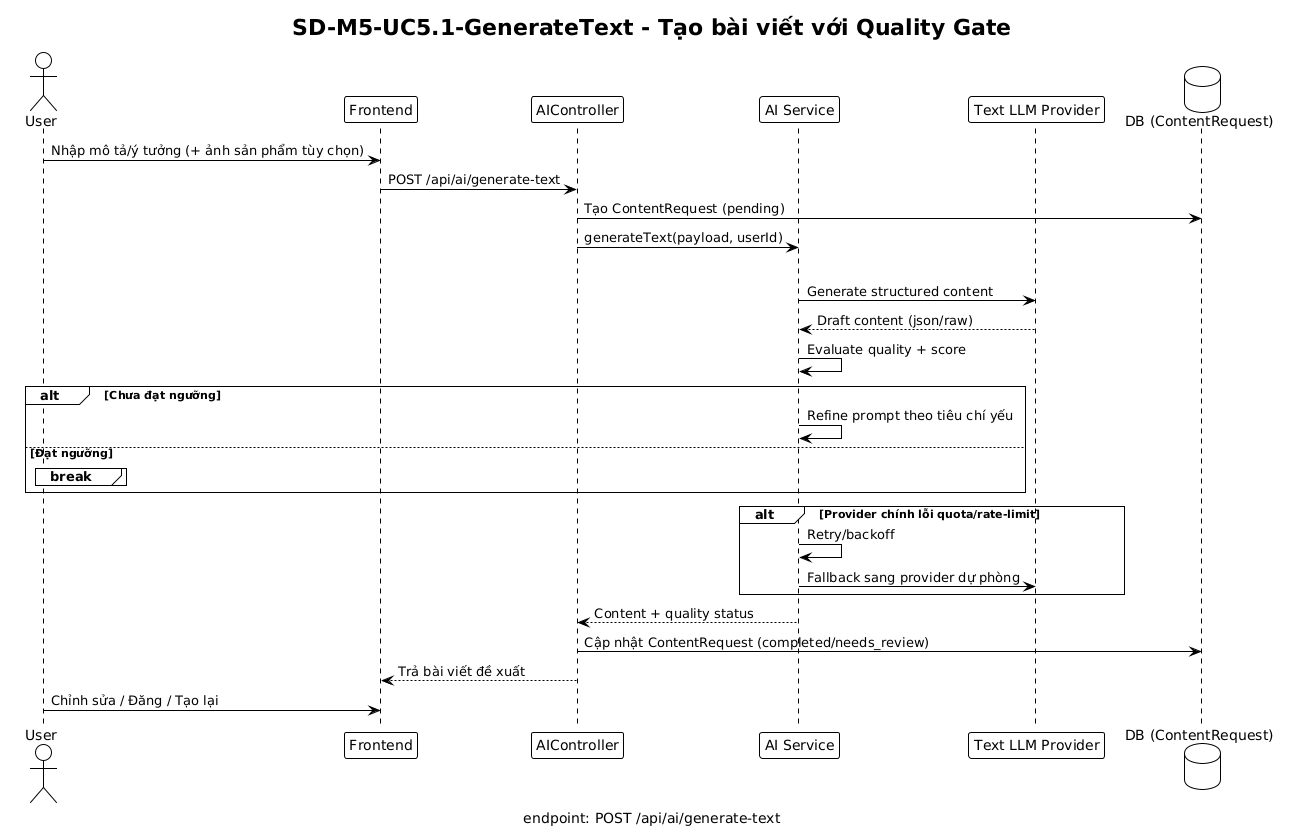
\includegraphics[width=\textwidth]{Images/Sequence diagrams/SD-M5-UC5.1-GenerateText.png}
  \caption{Sequence Diagram - Tạo bài viết với AI (SD-M5-UC5.1-GenerateText)}
\end{figure}

\begin{figure}[H]
  \centering
  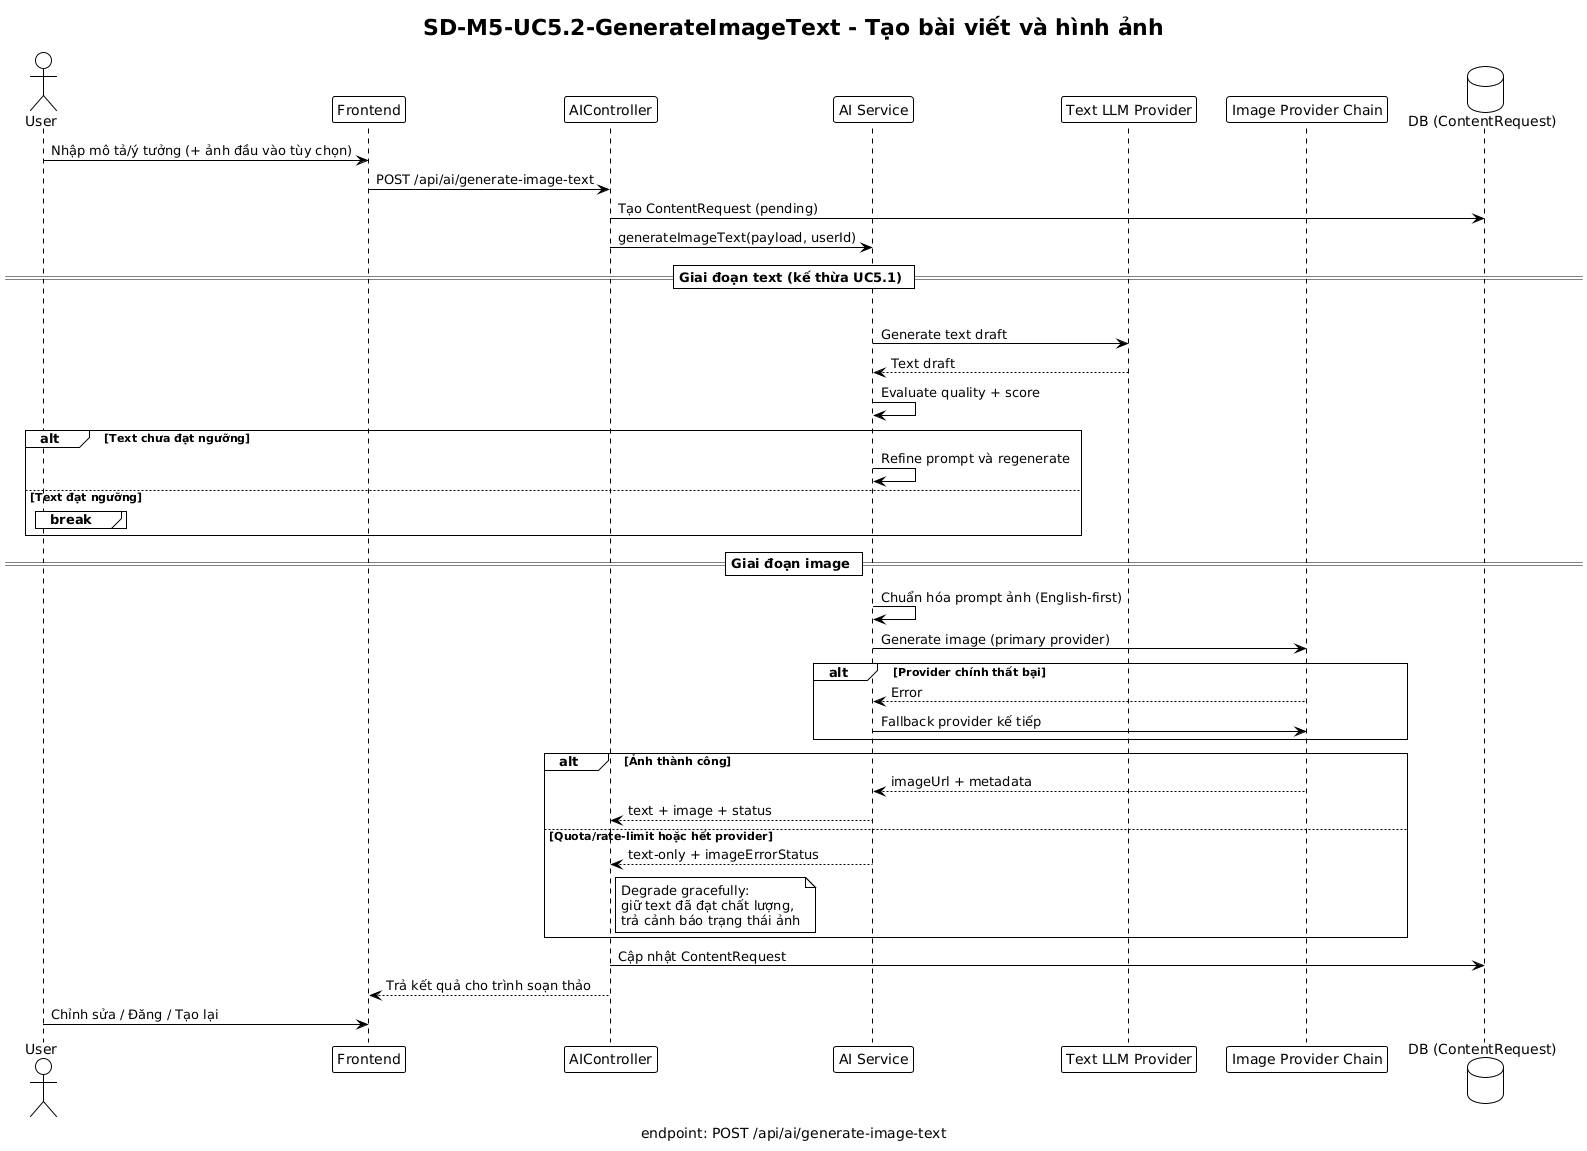
\includegraphics[width=\textwidth]{Images/Sequence diagrams/SD-M5-UC5.2-GenerateImageText.png}
  \caption{Sequence Diagram - Tạo bài viết và hình ảnh với AI (SD-M5-UC5.2-GenerateImageText)}
\end{figure}

\begin{figure}[H]
  \centering
  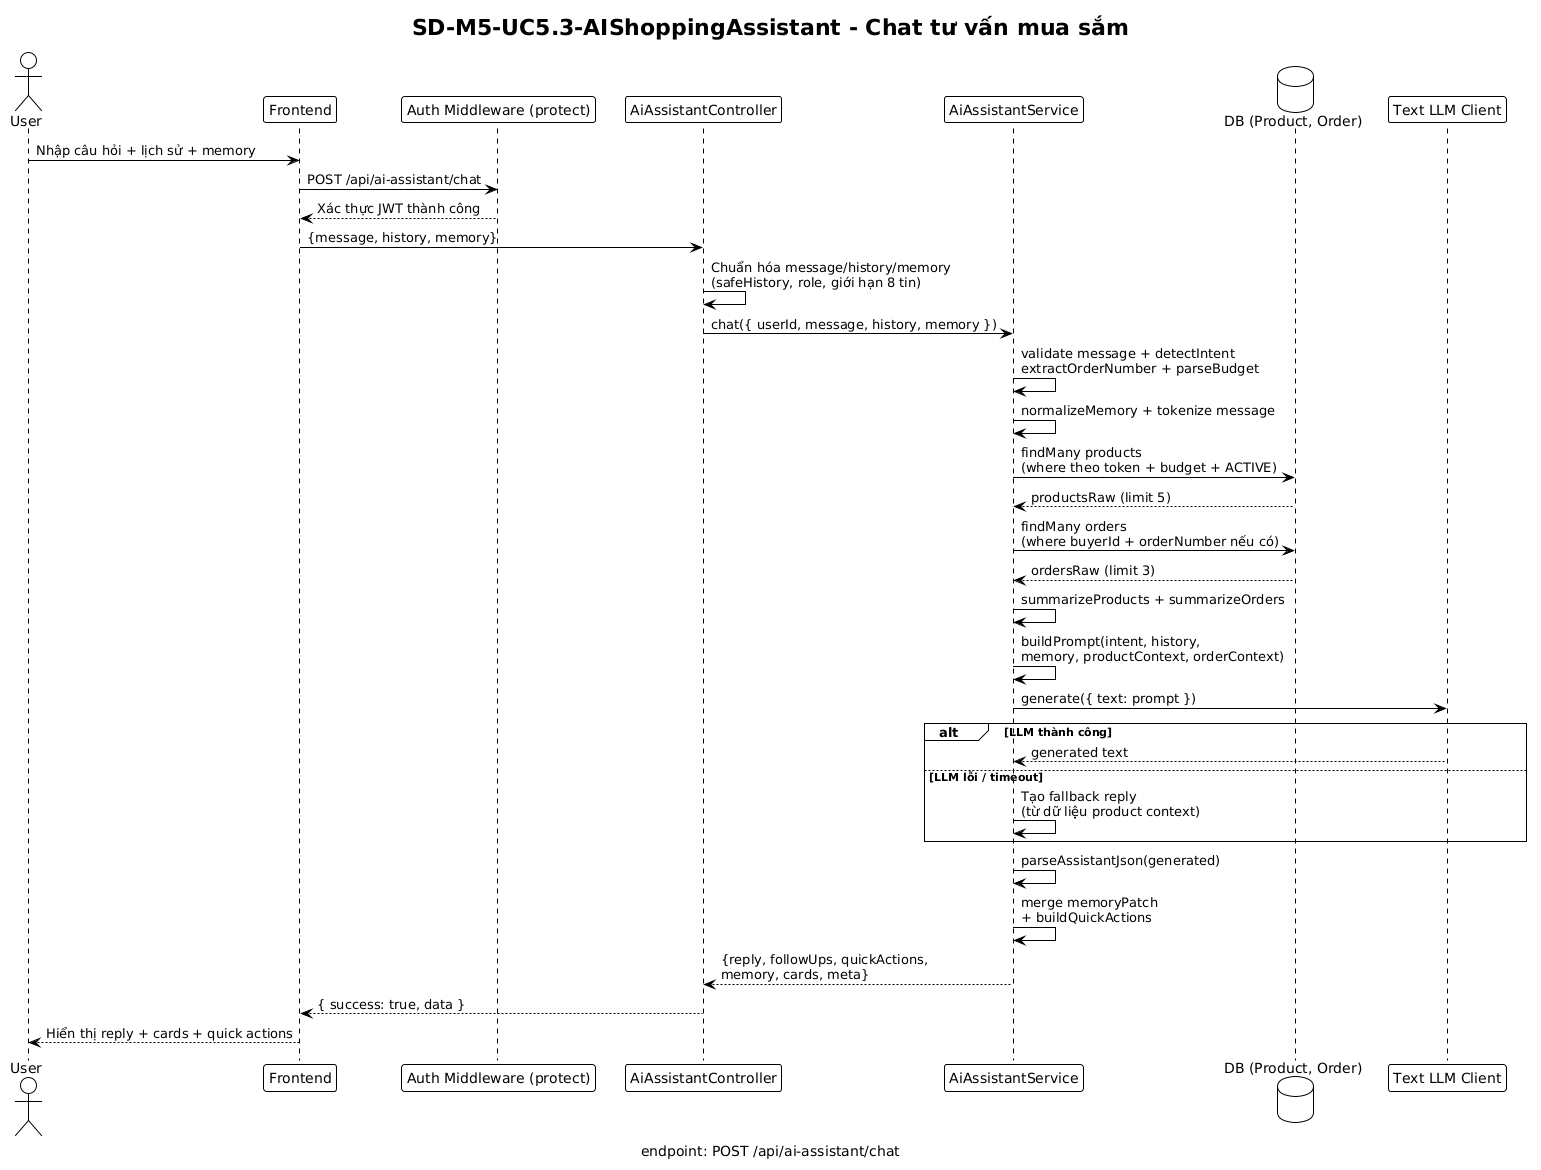
\includegraphics[width=\textwidth]{Images/Sequence diagrams/SD-M5-UC5.3-AIShoppingAssistant.png}
  \caption{Sequence Diagram - AI Shopping Assistant Chatbox (SD-M5-UC5.3-AIShoppingAssistant)}
\end{figure}

\subsection{Module 6 – Lên lịch và Điều phối Bài đăng}

Module này mô tả luồng tương tác trong tính năng lên lịch đăng bài: tạo lịch đăng, quản lý bài đăng đã lên lịch, và tự động xuất bản qua cron job. Các diagram thể hiện cách Frontend giao tiếp với PostController, Database và CronScheduler.

\subsubsection{SD-M6-PostScheduling}

Diagram này mô tả chuỗi tương tác trong quá trình lên lịch đăng bài và quản lý bài đăng đã lên lịch, bao gồm cả tác vụ tự động của cron job.

\textbf{UC6.1 – Lên lịch đăng bài:} Frontend gửi POST \texttt{/api/scheduled-posts} kèm nội dung, thời gian xuất bản (scheduledTime) và JWT token. ScheduledPostController xác thực, kiểm tra thời gian trong tương lai, lưu bài đăng với trạng thái \textit{scheduled} vào DB, trả về 201.

\textbf{UC6.2 – Quản lý bài đăng đã lên lịch:} Frontend gửi GET \texttt{/api/scheduled-posts} kèm JWT token. ScheduledPostController xác thực, truy vấn DB lấy danh sách bài đăng \textit{scheduled}, trả về danh sách. Để chỉnh sửa: Frontend gửi PUT \texttt{/api/scheduled-posts/:id}. Để đăng ngay: Frontend gửi POST \texttt{/api/scheduled-posts/:id/publish}. Để xóa: Frontend gửi DELETE \texttt{/api/scheduled-posts/:id}. Controller xử lý trong DB, trả về kết quả.

\textbf{Cron Job – Xuất bản tự động:} CronScheduler chạy định kỳ, truy vấn DB lấy scheduled posts có trạng thái \textit{scheduled} và thời gian đã đến. Scheduler tạo bản ghi Post tương ứng, cập nhật scheduled post thành \textit{published} và lưu publishedPostId.

\begin{figure}[H]
  \centering
  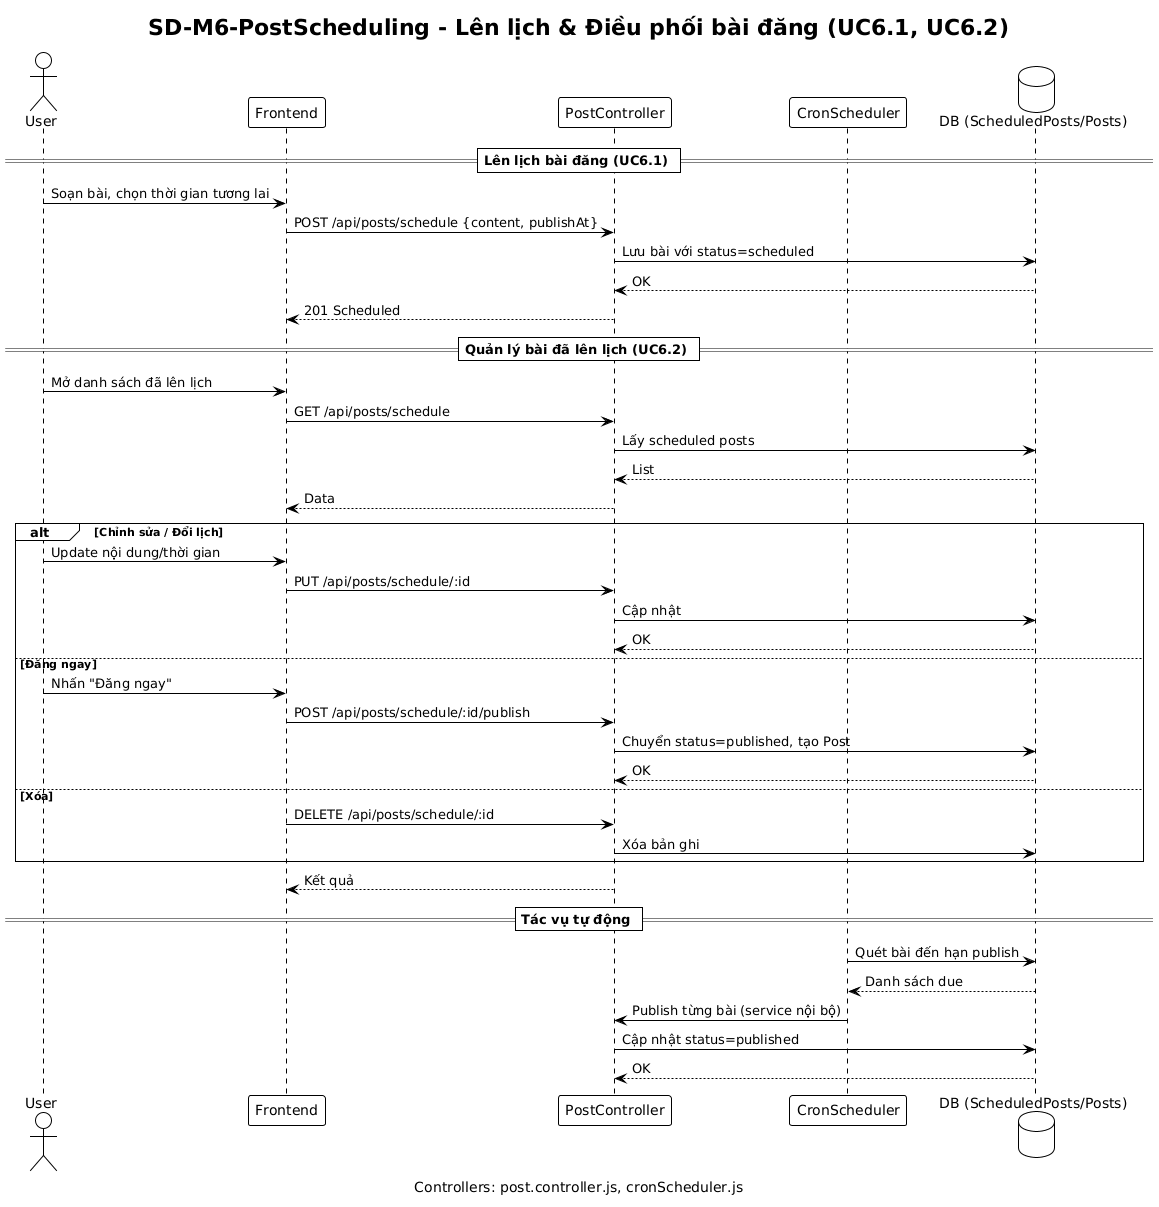
\includegraphics[width=\textwidth]{Images/Sequence diagrams/SD-M6-PostScheduling.png}
  \caption{Sequence Diagram - Lên lịch và Điều phối Bài đăng (SD-M6-PostScheduling)}
\end{figure}

\subsection{Module 7 – Hệ thống Thông báo}

Module này mô tả luồng tương tác trong hệ thống thông báo: tạo và gửi thông báo (tương tác xã hội, giao dịch), quản lý thông báo (xem, đánh dấu đã đọc, xóa), và cấu hình nhận thông báo. Các diagram thể hiện cách Frontend giao tiếp với NotificationController, NotificationService (Socket) và Database.

\subsubsection{SD-M7-NotificationSystem}

Diagram này mô tả chuỗi tương tác trong toàn bộ hệ thống thông báo, bao gồm bốn use case chính.

\textbf{UC7.1 – Thông báo tương tác:} Khi có sự kiện like, comment hoặc follow, service nghiệp vụ gọi NotificationService để tạo thông báo. NotificationService kiểm tra preference của người nhận, lưu thông báo vào DB và emit qua Socket.IO nếu người nhận online. Thông báo vẫn được lưu để hiển thị khi người nhận mở lại ứng dụng.

\textbf{UC7.2 – Thông báo giao dịch:} Khi có sự kiện giao dịch, hệ thống gọi NotificationController tạo thông báo. Controller lưu vào DB và gửi qua Socket đến Buyer/Seller. Nếu người nhận online và bật nhận, họ nhận real-time qua WebSocket.

\textbf{UC7.3 – Quản lý thông báo:} Frontend gửi GET \texttt{/api/notifications} kèm JWT token. NotificationController xác thực, truy vấn DB lấy danh sách thông báo (sắp xếp theo thời gian, mới nhất trước), trả về danh sách. Để đánh dấu đã đọc: Frontend gửi PATCH \texttt{/api/notifications/:id} với \texttt{\{read: true\}}. Để xóa: Frontend gửi DELETE \texttt{/api/notifications/:id}. Controller cập nhật/xóa trong DB, trả về 200.

\textbf{UC7.4 – Cài đặt thông báo:} Frontend gửi GET \texttt{/api/notifications/preferences} kèm JWT token. NotificationController xác thực, đọc cấu hình hiện tại từ privacySettings của user và trả về cấu hình. Để cập nhật: Frontend gửi PATCH \texttt{/api/notifications/preferences} kèm cấu hình mới và JWT token. Controller xác thực, lưu cấu hình vào DB, trả về 200. Cấu hình được áp dụng ngay lập tức.

\begin{figure}[H]
  \centering
  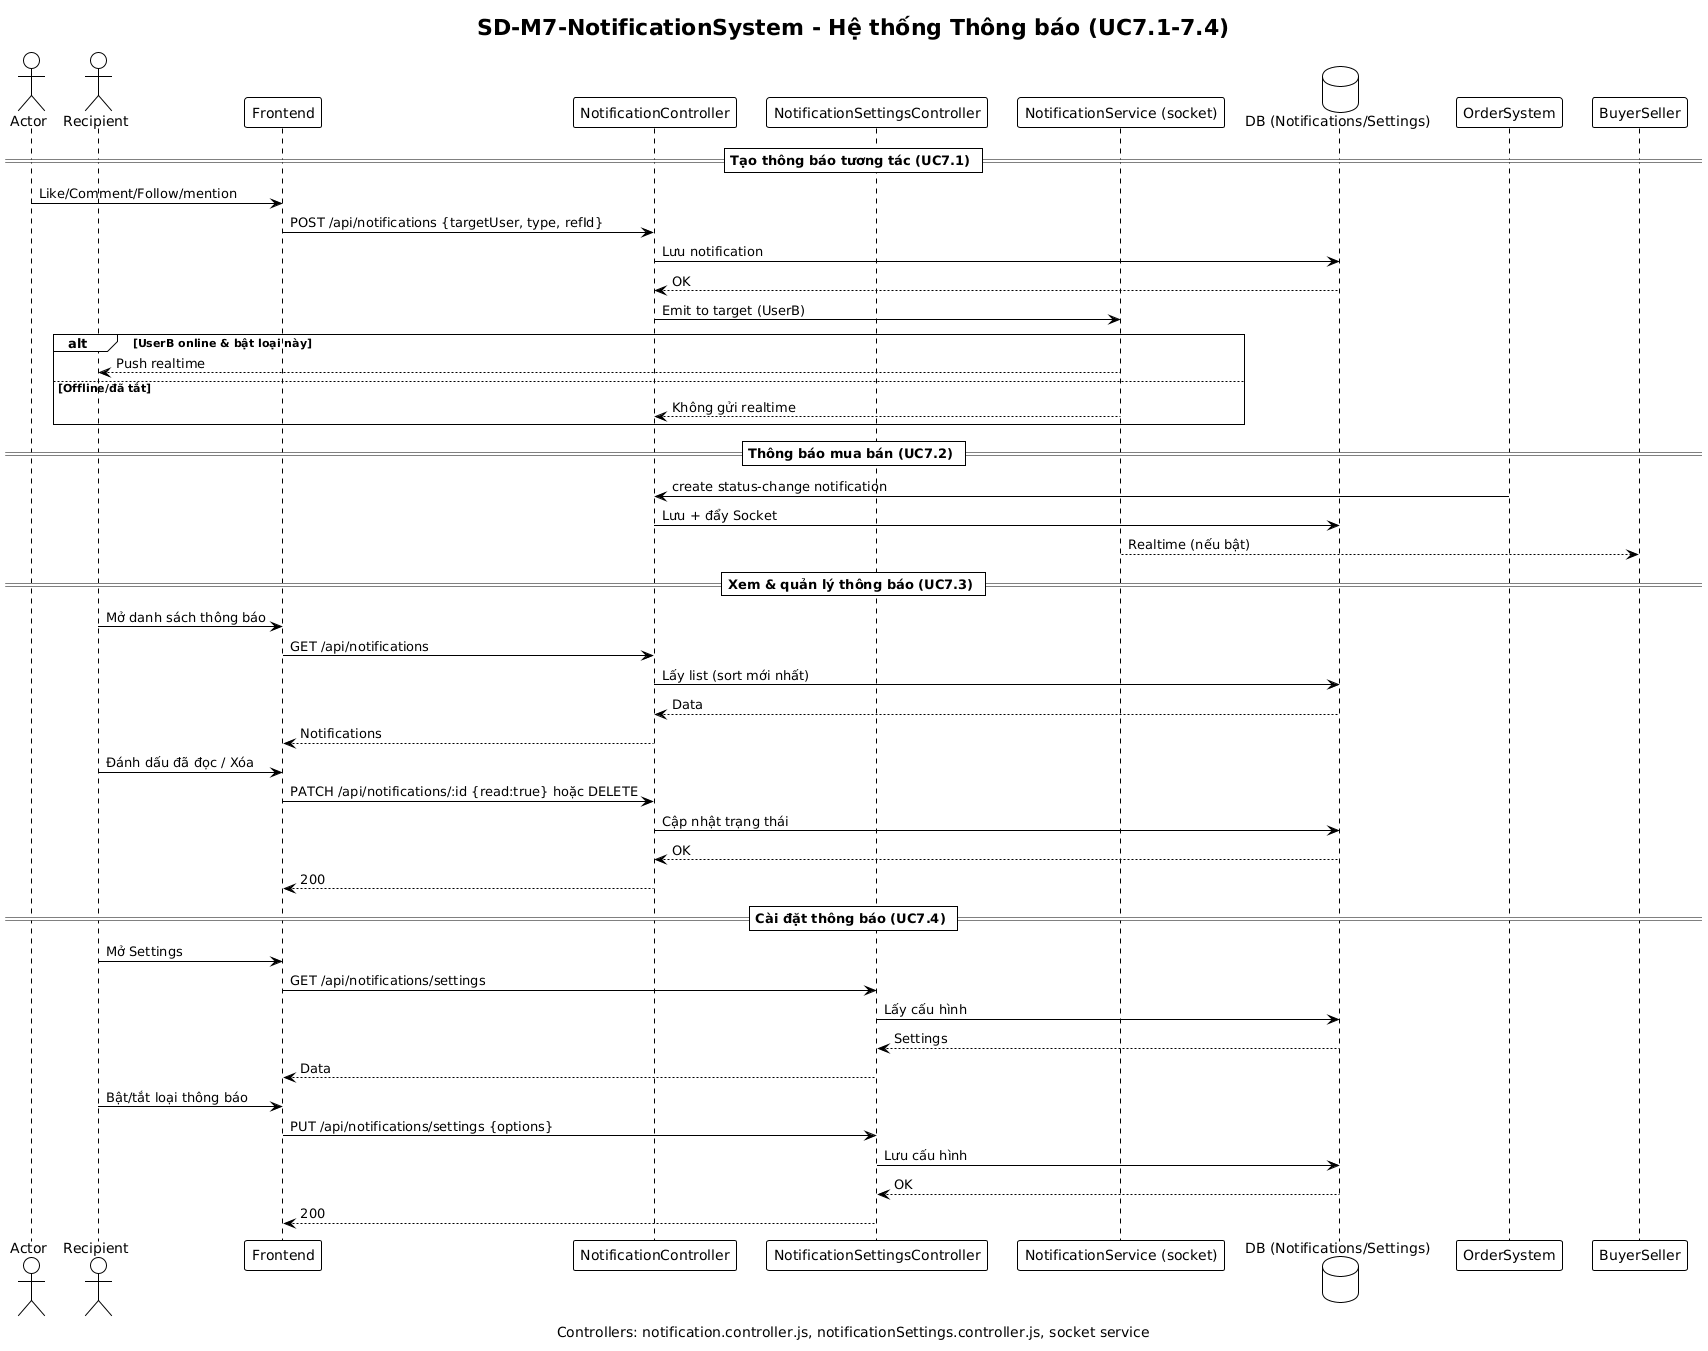
\includegraphics[width=\textwidth]{Images/Sequence diagrams/SD-M7-NotificationSystem.png}
  \caption{Sequence Diagram - Hệ thống Thông báo (SD-M7-NotificationSystem)}
\end{figure}


\section{Database design}
Dưới đây là mô tả chi tiết các entity, nêu ra vai trò, attribute và các relationship trong hệ thống.

\begin{figure}[H]
  \centering
  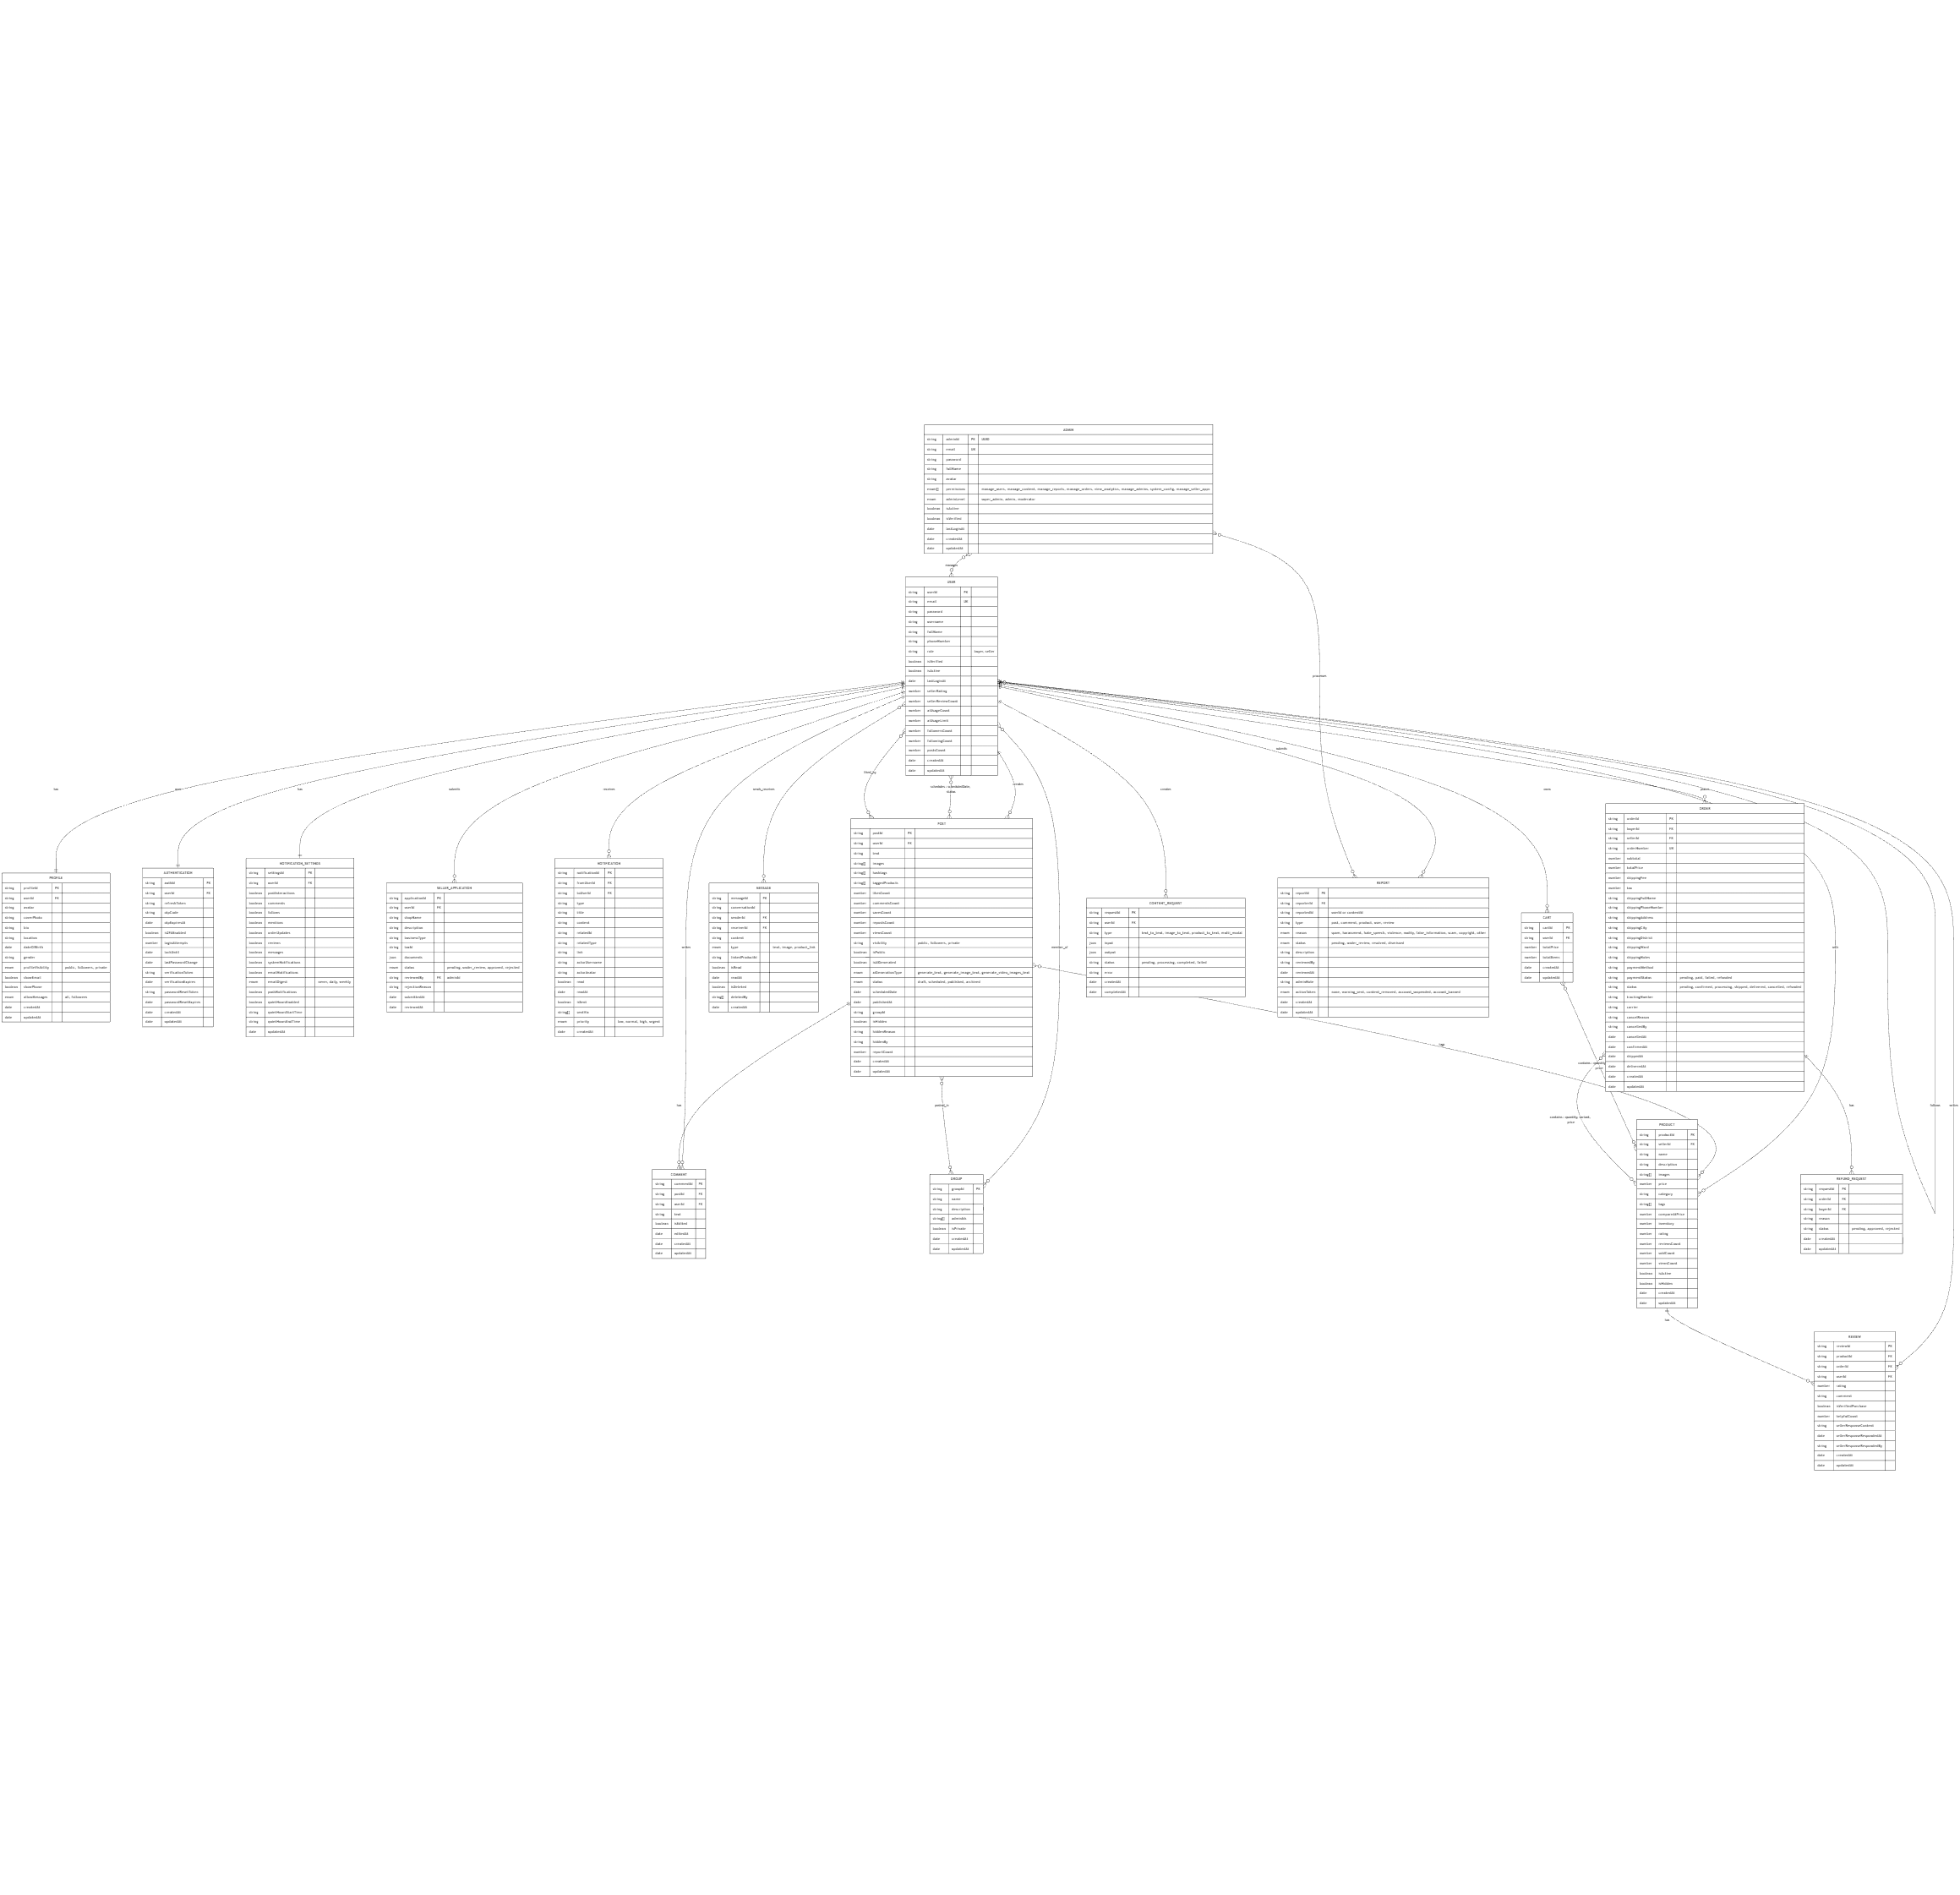
\includegraphics[width=\textwidth]{Images/ERD.png}
  \caption{Sơ đồ ERD (Entity Relationship Diagram) - Mô hình thực thể kết hợp của hệ thống}
  \label{fig:erd-diagram}
\end{figure}

\subsection{Thực thể (Entities)}
\paragraph{USER} Entity đại diện cho người dùng chung của hệ thống (buyer hoặc seller). Attributes: \textit{userId} (PK), email (UK), password, username, fullName, role (buyer/seller), isVerified, isActive, aiUsageCount (số lần đã sử dụng AI), aiUsageLimit (giới hạn số lần sử dụng AI), followersCount, followingCount, (...), createdAt, updatedAt.

\paragraph{PROFILE} Entity lưu trữ hồ sơ công khai/riêng tư gắn với người dùng. Attributes: \textit{profileId} (PK), \textit{userId} (FK), avatar, coverPhoto, bio, location, profileVisibility (public/followers/private), showEmail, allowMessages (all/followees), (...), createdAt, updatedAt.

\paragraph{AUTHENTICATION} Entity quản lý thông tin đăng nhập và bảo mật. Attributes: \textit{authId} (PK), \textit{userId} (FK), refreshToken, otpCode, otpExpiresAt, is2FAEnabled, loginAttempts, lockUntil, verificationToken, passwordResetToken, (...), createdAt, updatedAt.

\paragraph{NOTIFICATION\_SETTINGS} Entity lưu trữ cấu hình thông báo cá nhân. Attributes: \textit{settingsId} (PK), \textit{userId} (FK), postInteractions, comments, follows, orderUpdates, reviews, messages, emailNotifications, emailDigest (never/daily/weekly), pushNotifications, quietHoursEnabled, (...), updatedAt.

\paragraph{NOTIFICATION} Entity lưu trữ bản ghi thông báo gửi tới người dùng. Attributes: \textit{notificationId} (PK), fromUserId (FK), toUserId (FK), type, title, content, relatedId, relatedType, link, read, readAt, priority (low/normal/high/urgent), (...), createdAt.

\paragraph{POST} Entity đại diện cho bài viết của người dùng. Attributes: \textit{postId} (PK), \textit{userId} (FK), text (nội dung văn bản), images[] (danh sách ảnh), hashtags[], taggedProducts[], likesCount, commentsCount, viewsCount, visibility (public/followers/private), isAIGenerated (được tạo bởi AI), aiGenerationType (generate\_text/generate\_image\_text/generate\_video\_images\_text - loại tạo nội dung AI), status (draft/scheduled/published/archived), scheduledDate, publishedAt, (...), createdAt, updatedAt.

\paragraph{COMMENT} Entity đại diện cho bình luận trên bài viết. Attributes: \textit{commentId} (PK), \textit{postId} (FK), \textit{userId} (FK), text, isEdited, editedAt, createdAt, updatedAt.

\paragraph{GROUP} Entity đại diện cho nhóm cộng đồng. Attributes: \textit{groupId} (PK), name, description, adminIds[], isPrivate, createdAt, updatedAt.

\paragraph{MESSAGE} Entity lưu trữ tin nhắn giữa người dùng. Attributes: \textit{messageId} (PK), conversationId, senderId (FK), receiverId (FK), content, type (text/image/product\_link), linkedProductId, isRead, readAt, (...), createdAt.

\paragraph{PRODUCT} Entity đại diện cho sản phẩm do người bán đăng. Attributes: \textit{productId} (PK), sellerId (FK), name, description, images[], price, category, tags[], compareAtPrice, inventory, rating, reviewsCount, soldCount, viewsCount, isActive, (...), createdAt, updatedAt.

\paragraph{CART} Entity đại diện cho giỏ hàng của người mua. Attributes: \textit{cartId} (PK), \textit{userId} (FK), totalPrice, totalItems, createdAt, updatedAt.

\paragraph{ORDER} Entity đại diện cho đơn hàng giữa người mua và người bán. Attributes: \textit{orderId} (PK), buyerId (FK), sellerId (FK), orderNumber (UK), subtotal, totalPrice, shippingFee, shippingAddress, shippingCity, paymentMethod, paymentStatus (pending/paid/failed/refunded), status (pending/confirmed/processing/shipped/delivered/cancelled/refunded), trackingNumber, refund\_status, refund\_reason, (...), createdAt, updatedAt.

\paragraph{REVIEW} Entity đại diện cho đánh giá sản phẩm gắn với đơn. Attributes: \textit{reviewId} (PK), productId (FK), orderId (FK), userId (FK), rating, comment, isVerifiedPurchase, helpfulCount, sellerResponseContent, (...), createdAt, updatedAt.

\paragraph{REFUND\_REQUEST} Entity đại diện cho yêu cầu hoàn tiền cho đơn. \textbf{Lưu ý:} Trong schema thực tế, các trường refund được tích hợp vào bảng \textit{orders} (refund\_status, refund\_reason, refund\_requested\_at, refund\_processed\_at, refund\_processed\_by).

\paragraph{CONTENT\_REQUEST} Entity lưu trữ yêu cầu tạo nội dung AI. Attributes: \textit{requestId} (PK), userId (FK), type (generate\_text/generate\_image\_text/generate\_video\_images\_text - loại yêu cầu), input (json - dữ liệu đầu vào), output (json - kết quả đầu ra), status (pending/processing/completed/failed), error, createdAt, completedAt.

\paragraph{REPORT} Entity lưu trữ báo cáo vi phạm. Attributes: \textit{reportId} (PK), reporterId (FK), reportedId, type (post/comment/product/user/review), reason (spam/harassment/hate\_speech/violence/nudity/false\_information/scam/copyright/other), status (pending/under\_review/resolved/dismissed), description, reviewedBy, actionTaken (none/warning\_sent/content\_removed/account\_suspended/account\_banned), (...), createdAt, updatedAt.

\paragraph{SELLER\_APPLICATION} Entity lưu trữ hồ sơ đăng ký trở thành người bán. Attributes: \textit{applicationId} (PK), userId (FK), shopName, description, businessType, taxId, documents (json), status (pending/under\_review/approved/rejected), reviewedBy, rejectionReason, submittedAt, reviewedAt.

\paragraph{ADMIN} Entity đại diện cho tài khoản quản trị. Attributes: \textit{adminId} (PK, UUID), email (UK), password, fullName, avatar, permissions[] (manage\_users/manage\_content/manage\_reports/manage\_orders/view\_analytics/manage\_admins/system\_config/manage\_seller\_apps), adminLevel (super\_admin/admin/moderator), isActive, isVerified, lastLoginAt, createdAt, updatedAt.

\subsection{Mối quan hệ (Relationships)}
\begin{itemize}
  \item \textbf{USER -- PROFILE}: 1:1. Mỗi USER có đúng một PROFILE; mỗi PROFILE chỉ thuộc một USER.
  \item \textbf{USER -- AUTHENTICATION}: 1:1. Lưu token/OTP và cấu hình 2FA cho đúng một USER.
  \item \textbf{USER -- NOTIFICATION\_SETTINGS}: 1:1. Mỗi USER có cấu hình thông báo riêng.
  \item \textbf{USER -- NOTIFICATION}: 1:N. Một USER nhận nhiều thông báo qua toUserId; fromUserId ghi nhận tác nhân phát sinh.
  \item \textbf{USER -- SELLER\_APPLICATION}: 1:N. Người dùng có thể nộp nhiều đơn đăng ký bán.
  \item \textbf{ADMIN -- USER}: N:M (quản lý). ADMIN có thể quản lý nhiều USER và ngược lại (phân ca/phạm vi).
  \item \textbf{USER -- USER (follow)}: N:M. Người dùng có thể theo dõi lẫn nhau.
  \item \textbf{POST -- COMMENT}: 1:N. Một POST có nhiều COMMENT; COMMENT thuộc duy nhất một POST.
  \item \textbf{USER -- POST}: 1:N. Người dùng tạo nhiều POST; mỗi POST thuộc một USER.
  \item \textbf{USER -- COMMENT}: 1:N. Người dùng viết nhiều COMMENT.
  \item \textbf{POST -- USER (liked\_by)}: N:M. Một bài có nhiều người thích; một người thích nhiều bài.
  \item \textbf{POST -- GROUP (posted\_in)}: N:M. Bài viết có thể được đăng trong nhiều GROUP; GROUP chứa nhiều bài.
  \item \textbf{POST -- PRODUCT (tags)}: N:M. Bài viết có thể gắn nhiều sản phẩm; sản phẩm có thể được tag ở nhiều bài.
  \item \textbf{USER -- GROUP (member\_of)}: N:M. Người dùng có thể tham gia nhiều nhóm; nhóm có nhiều thành viên.
  \item \textbf{USER -- MESSAGE}: N:M. Một USER gửi/nhận nhiều MESSAGE; mỗi MESSAGE có sender và receiver.
  \item \textbf{USER -- POST (schedules)}: N:M qua thuộc tính scheduling. Một USER có thể lên lịch nhiều POST; một POST có thể có bản ghi lịch.
  \item \textbf{USER -- PRODUCT}: 1:N. Một người bán đăng nhiều PRODUCT; mỗi PRODUCT thuộc một seller.
  \item \textbf{CART -- PRODUCT}: N:M. Một CART chứa nhiều PRODUCT (kèm quantity/variant/price trên dòng giỏ); một PRODUCT có thể nằm trong nhiều CART.
  \item \textbf{ORDER -- PRODUCT}: N:M. Một ORDER chứa nhiều PRODUCT (dòng hàng gồm quantity/variant/price); một PRODUCT xuất hiện trong nhiều ORDER.
  \item \textbf{USER -- CART}: 1:N (thiết kế cho phép nhiều giỏ theo phiên; thực tế thường 1). Mỗi CART thuộc một USER.
  \item \textbf{USER -- ORDER}: 1:N. Người mua có nhiều ORDER; mỗi ORDER gắn với một buyer. Đồng thời ORDER giữ sellerId để biết người bán.
  \item \textbf{USER -- REVIEW}: 1:N. Người dùng viết nhiều REVIEW.
  \item \textbf{PRODUCT -- REVIEW}: 1:N. Một PRODUCT có nhiều REVIEW.
  \item \textbf{ORDER -- REFUND\_REQUEST}: 1:N. Một ORDER có thể phát sinh nhiều REFUND\_REQUEST.
  \item \textbf{USER -- REFUND\_REQUEST}: 1:N. Người mua gửi nhiều yêu cầu hoàn.
  \item \textbf{USER -- CONTENT\_REQUEST}: 1:N. Người dùng tạo nhiều yêu cầu AI; mỗi yêu cầu thuộc một USER.
  \item \textbf{USER -- REPORT}: 1:N. Người dùng có thể gửi nhiều REPORT; mỗi REPORT có một reporter.
  \item \textbf{ADMIN -- REPORT}: N:M. Nhiều ADMIN có thể xử lý các REPORT, mỗi REPORT có thể được giao/lưu vết nhiều admin.
\end{itemize}

\subsection{Chuyển đổi từ ERD sang Database Schema}

Quá trình chuyển đổi từ mô hình ERD sang database schema PostgreSQL đã được thực hiện với các quyết định thiết kế cụ thể để tối ưu performance, đảm bảo data integrity và hỗ trợ các tính năng của hệ thống.

\subsubsection{Quyết định về cấu trúc bảng (Table Structure)}

\paragraph{Junction Tables cho quan hệ N:M}
Để hỗ trợ các relationship N:M, hệ thống đã tách thành các junction table riêng biệt thay vì sử dụng array:

\begin{itemize}
  \item \textbf{post\_likes}: Lưu trữ relationship giữa POST và USER (liked\_by). Mỗi record gồm post\_id, user\_id và created\_at. Có UNIQUE constraint (post\_id, user\_id) để đảm bảo một người dùng chỉ like một bài viết một lần.
  \item \textbf{post\_saves}: Tương tự cho chức năng lưu bài viết (bookmark).
  \item \textbf{post\_reposts}: Lưu trữ các bài viết được chia sẻ lại (repost).
  \item \textbf{review\_helpful\_votes}: Lưu trữ các vote "hữu ích" cho đánh giá sản phẩm.
  \item \textbf{group\_members}: Quản lý thành viên của nhóm với role (member/admin/moderator), thay vì chỉ dùng adminIds[] trong GROUP.
  \item \textbf{user\_follows}: Relationship follow giữa người dùng với UNIQUE constraint (follower\_id, following\_id) và CHECK constraint để tránh tự follow.
  \item \textbf{user\_blocks}: Relationship block giữa người dùng (không có trong ERD nhưng cần thiết cho tính năng chặn người dùng).
\end{itemize}

\paragraph{Denormalization}
Một số quyết định gộp bảng để tối ưu query performance:

\begin{itemize}
  \item \textbf{REFUND\_REQUEST → orders}: Thay vì tạo bảng REFUND\_REQUEST riêng như trong ERD, các trường refund được tích hợp trực tiếp vào bảng \textit{orders}:
  \begin{itemize}
    \item refund\_requested (BOOLEAN)
    \item refund\_status (pending/approved/rejected)
    \item refund\_reason (TEXT)
    \item refund\_requested\_at, refund\_processed\_at (TIMESTAMP)
    \item refund\_processed\_by (FK → users)
  \end{itemize}
  Lý do: Mỗi đơn hàng chỉ có tối đa một yêu cầu hoàn tiền, việc gộp giảm số lượng JOIN và tăng query performance.
\end{itemize}

\paragraph{Supporting Tables}
Các bảng hỗ trợ được tách để quản lý metadata và lịch sử:

\begin{itemize}
  \item \textbf{product\_images}: Tách từ images[] trong PRODUCT để lưu metadata (url, public\_id, is\_primary, width, height) và hỗ trợ quản lý ảnh tốt hơn.
  \item \textbf{post\_images}: Tương tự cho POST (mặc dù posts vẫn giữ images[] để backward compatibility).
  \item \textbf{review\_images}: Ảnh đính kèm trong đánh giá sản phẩm.
  \item \textbf{report\_screenshots}: Ảnh chụp màn hình trong báo cáo vi phạm.
  \item \textbf{order\_status\_history}: Lưu lịch sử thay đổi trạng thái đơn hàng với timestamp, note và updated\_by để audit trail.
  \item \textbf{product\_variants} và \textbf{product\_variant\_options}: Hỗ trợ biến thể sản phẩm (size, color, etc.) với giá và tồn kho riêng.
\end{itemize}

\subsubsection{Sơ đồ Relational Mapping}
Hình \ref{fig:relational-mapping} mô tả sơ đồ relational mapping của hệ thống, thể hiện tất cả các bảng và mối quan hệ giữa chúng thông qua Primary Keys (PK) và Foreign Keys (FK). Sơ đồ này được tạo từ database schema PostgreSQL thực tế, bao gồm các junction tables cho quan hệ N:M và các supporting tables đã được mô tả ở trên.

\begin{figure}[H]
  \centering
  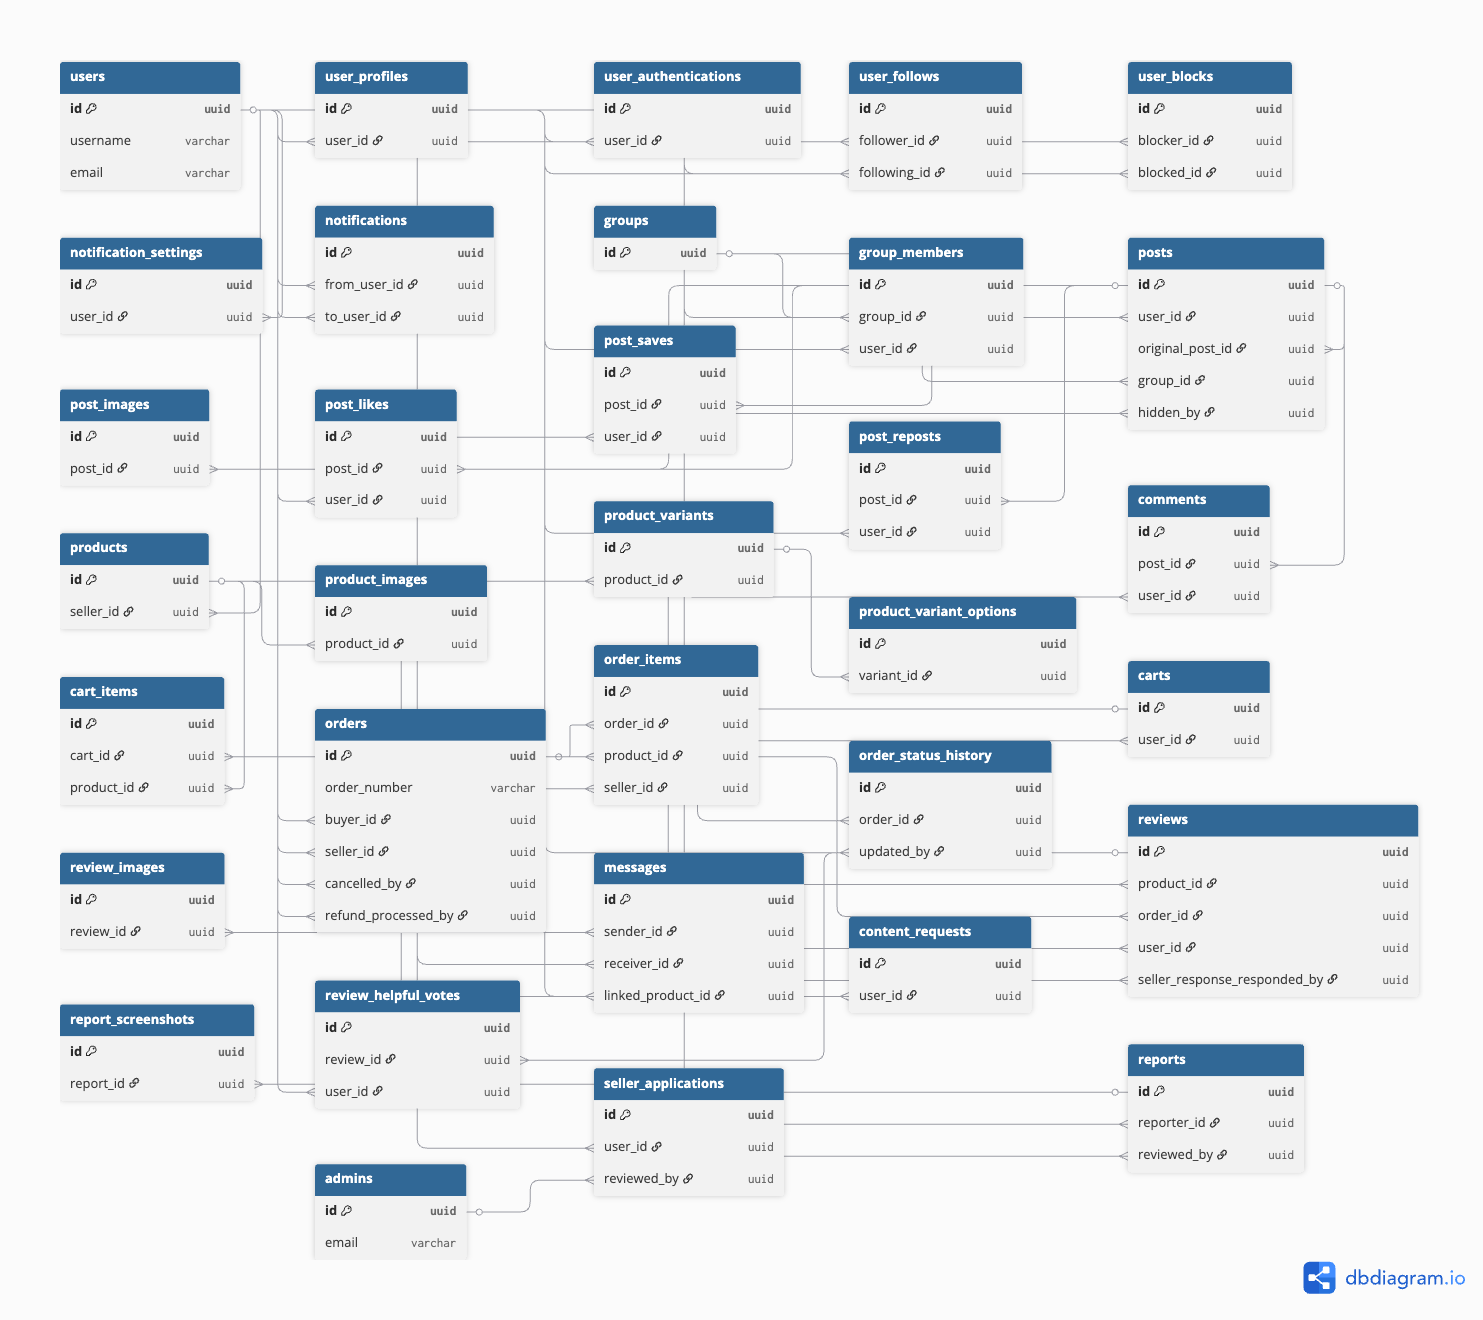
\includegraphics[width=\textwidth]{Images/Relation-Mapping.png}
  \caption{Sơ đồ Relational Mapping - Các bảng và mối quan hệ trong database schema}
  \label{fig:relational-mapping}
\end{figure}


\section{Architecture design}
\subsection{Architectural pattern}

Dự án sử dụng mô hình \textbf{MVCS}. Kiến trúc chuẩn của \textbf{MVCS} được thể hiện trong \ref{fig:mvcs-pattern}:

\begin{figure}[htbp]
    \centering
    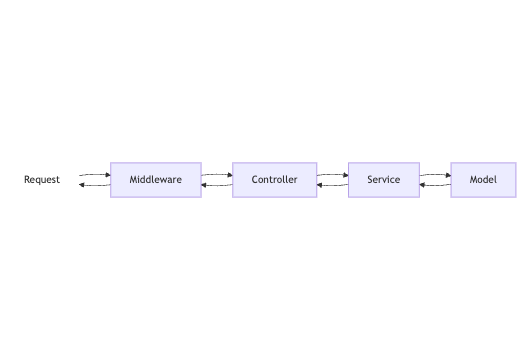
\includegraphics[width=0.8\textwidth]{Images/MVCS.png}
    \caption{MVCS pattern}
    \label{fig:mvcs-pattern}
\end{figure}

\textbf{MVCS} là viết tắt của \textbf{Model-View-Controller-Service}. Mô hình này cho phép lập trình viên định nghĩa trước sự tương tác giữa các phần code và dễ dàng chỉnh sửa bằng cách chia code thành các \textbf{layer} theo chức năng. Kiến trúc này không thuộc về bất kỳ ngôn ngữ lập trình hay framework cụ thể nào. \textbf{Pattern} này tách biệt \textbf{Database} hoặc \textbf{networking interaction} khỏi \textbf{Controller}. Mỗi phần đóng vai trò quan trọng trong việc phát triển ứng dụng.

\begin{itemize}
    \item \textbf{View Layer}: Đại diện cho cách dữ liệu được render lên giao diện người dùng. Trong dự án này, \textbf{View Layer} được xây dựng bằng \textbf{React.js} với các \textbf{Router} quản lý navigation và các \textbf{Component} hiển thị dữ liệu.
    \item \textbf{Controller Layer}: Chịu trách nhiệm chỉ nhận \textbf{request} và hiển thị kết quả của thao tác. \textbf{Controller} được sử dụng để giao tiếp giữa \textbf{Model}, \textbf{Service} và \textbf{View}. Trong \textbf{Backend Node.js}, các \textbf{Controller} như \textbf{Auth Controller}, \textbf{User Controller}, \textbf{Post Controller} xử lý các request từ \textbf{Frontend} và trả về \textbf{response} tương ứng.
    \item \textbf{Service Layer}: Còn được gọi là \textbf{Business Layer}, chứa các chức năng tạo nên core của ứng dụng, do đó trở nên \textbf{highly reusable} cho controllers và services. \textbf{Service Layer} xử lý \textbf{business logic} phức tạp, tách biệt khỏi \textbf{Controller} để dễ dàng maintain và test.
    \item \textbf{Model Layer}: Chịu trách nhiệm định nghĩa cách \textbf{data model} được định nghĩa. \textbf{Model Layer} sử dụng \textbf{Sequelize ORM} để ánh xạ các \textbf{entity} trong database như \textbf{User}, \textbf{Post}, \textbf{Product}, \textbf{Order}, \textbf{Message} và \textbf{Notification}.
\end{itemize}

\subsection{Architecture diagram}

\ref{fig:architecture-diagram} minh họa tổng quan cách chúng tôi lên kế hoạch triển khai hệ thống. Đối với \textbf{frontend}, tất cả các thiết kế đã được thực hiện với \textbf{Figma} sẽ được implement bằng \textbf{React.js} và cấu trúc được tổ chức như trong hình. \textbf{Frontend} được kết nối với \textbf{Backend Node.js} thông qua \textbf{HTTP request} và \textbf{WebSocket connection}.

\begin{figure}[htbp]
    \centering
    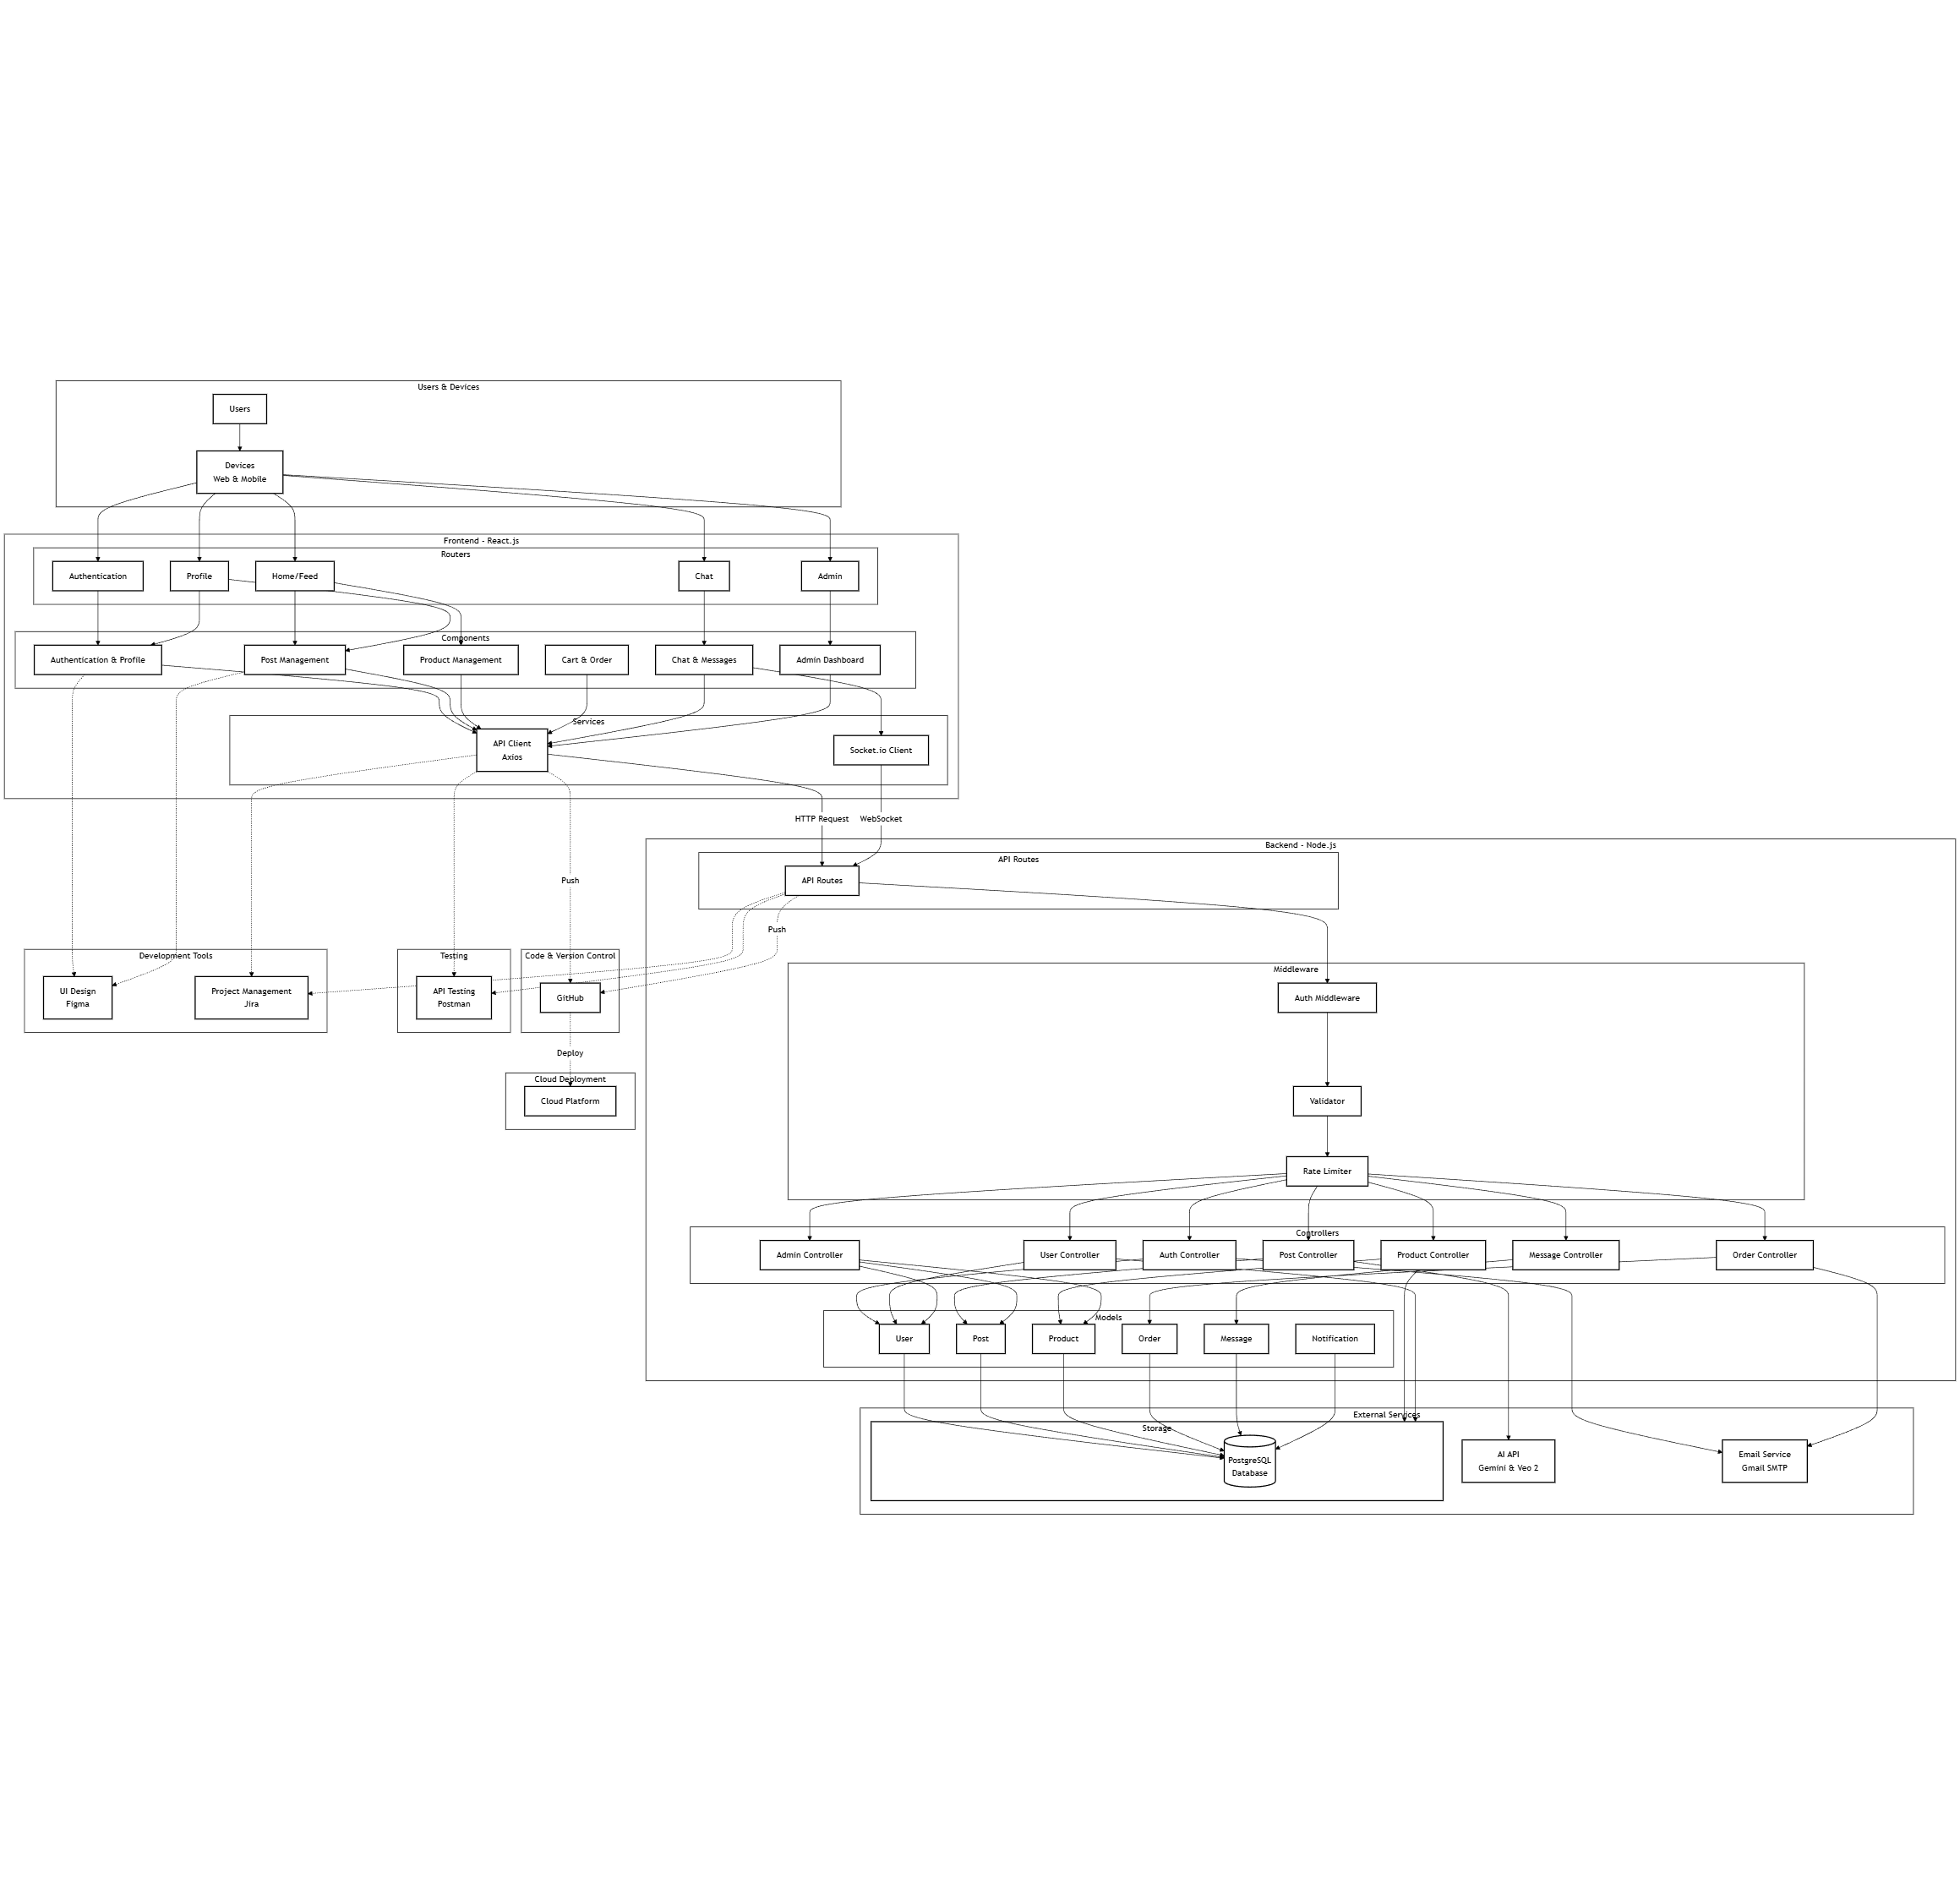
\includegraphics[width=1.0\textwidth]{Images/Architecture Diagram.png}
    \caption{Architecture Diagram for the system}
    \label{fig:architecture-diagram}
\end{figure}

\paragraph{Frontend Structure} Cấu trúc \textbf{Frontend} được tổ chức thành các thành phần chính:

\begin{itemize}
    \item \textbf{Routers}: Quản lý navigation giữa các trang
    \begin{itemize}
        \item \textbf{Authentication}: Trang xác thực người dùng
        \item \textbf{Home/Feed}: Trang chủ và bảng tin
        \item \textbf{Profile}: Trang hồ sơ người dùng
        \item \textbf{Chat}: Trang nhắn tin
        \item \textbf{Admin}: Trang quản trị
    \end{itemize}
    \item \textbf{Components}: Được tổ chức theo chức năng
    \begin{itemize}
        \item \textbf{Authentication \& Profile}: Xác thực và quản lý hồ sơ
        \item \textbf{Post Management}: Quản lý bài viết
        \item \textbf{Product Management}: Quản lý sản phẩm
        \item \textbf{Cart \& Order}: Giỏ hàng và đơn hàng
        \item \textbf{Chat \& Messages}: Tin nhắn và cuộc trò chuyện
        \item \textbf{Admin Dashboard}: Bảng điều khiển quản trị
    \end{itemize}
    \item \textbf{Services}: Kết nối với Backend
    \begin{itemize}
        \item \textbf{API Client (Axios)}: Thực hiện \textbf{HTTP request}
        \item \textbf{Socket.io Client}: Thiết lập kết nối \textbf{WebSocket} cho các tính năng \textbf{real-time}
    \end{itemize}
\end{itemize}

\paragraph{Backend Structure} \textbf{Backend} được xây dựng bằng \textbf{Node.js} với \textbf{Express.js framework}. Cấu trúc bao gồm:

\begin{itemize}
    \item \textbf{API Routes}: Đóng vai trò \textbf{entry point} nhận các request từ \textbf{Frontend}
    \item \textbf{Middleware}: Xử lý request qua chuỗi middleware
    \begin{itemize}
        \item \textbf{Auth Middleware}: Xác thực \textbf{JWT} và quản lý \textbf{session}
        \item \textbf{Validator}: Kiểm tra và validate dữ liệu đầu vào
        \item \textbf{Rate Limiter}: Giới hạn số lượng request để bảo vệ hệ thống
    \end{itemize}
    \item \textbf{Controllers}: Xử lý logic nghiệp vụ
    \begin{itemize}
        \item \textbf{Auth Controller}: Xử lý xác thực
        \item \textbf{User Controller}: Quản lý người dùng
        \item \textbf{Post Controller}: Quản lý bài viết
        \item \textbf{Product Controller}: Quản lý sản phẩm
        \item \textbf{Order Controller}: Quản lý đơn hàng
        \item \textbf{Message Controller}: Quản lý tin nhắn
        \item \textbf{Admin Controller}: Quản lý quản trị
    \end{itemize}
    \item \textbf{Models}: Đại diện cho các entity trong hệ thống
    \begin{itemize}
        \item \textbf{User}: Người dùng
        \item \textbf{Post}: Bài viết
        \item \textbf{Product}: Sản phẩm
        \item \textbf{Order}: Đơn hàng
        \item \textbf{Message}: Tin nhắn
        \item \textbf{Notification}: Thông báo
        \item Các Model hỗ trợ khác
    \end{itemize}
\end{itemize}

\paragraph{Database} Các \textbf{Model} này kết nối trực tiếp với database \textbf{PostgreSQL} thông qua \textbf{Sequelize ORM} để thực hiện các thao tác \textbf{CRUD} (Create, Read, Update, Delete).

\paragraph{Code \& Version Control} Để quản lý code và version, nhóm sử dụng \textbf{GitHub} và từ đó chúng tôi lên kế hoạch triển khai website thông qua \textbf{Cloud Platform} sử dụng các dịch vụ:

\begin{itemize}
    \item \textbf{Elastic Beanstalk}: Triển khai và quản lý ứng dụng
    \item \textbf{CodePipeline}: Tự động hóa quy trình CI/CD
    \item \textbf{Amazon RDS}: Quản lý database
\end{itemize}

Tất cả đều được cung cấp bởi các nhà cung cấp cloud.

\paragraph{Testing \& Development Tools} Hệ thống sử dụng các công cụ hỗ trợ:

\begin{itemize}
    \item \textbf{Testing}:
    \begin{itemize}
        \item \textbf{Postman}: Kiểm tra và đánh giá \textbf{API}
    \end{itemize}
    \item \textbf{Development Tools}:
    \begin{itemize}
        \item \textbf{Jira Software}: Bug tracking và project management
    \end{itemize}
\end{itemize}

\paragraph{External Services} Hệ thống tích hợp với các dịch vụ bên ngoài:

\begin{itemize}
    \item \textbf{AI API (Google Gemini \& Veo 2)}: Tạo nội dung đa phương thức (văn bản, hình ảnh, video ngắn)
    \item \textbf{File Storage (Cloudinary)}: Lưu trữ và quản lý hình ảnh
    \item \textbf{Email Service (Gmail SMTP)}: Gửi email xác thực và thông báo
\end{itemize}


\section{Thiết kế Pipeline AI Content Generation}
Phần này trình bày chi tiết thiết kế pipeline tạo nội dung AI cho hệ thống Social Commerce, bao gồm quy trình xây dựng prompt, tiêu chí đánh giá chất lượng kết quả, và chiến lược cải thiện khi kết quả chưa đạt yêu cầu.

\subsection{Tổng quan Pipeline}

Pipeline tạo nội dung AI được thiết kế theo mô hình \textbf{vòng lặp đánh giá -- cải thiện (Evaluate--Refine Loop)}, đảm bảo chất lượng đầu ra trước khi trả kết quả cho người dùng. Pipeline gồm 7 giai đoạn chính:

\begin{enumerate}
    \item \textbf{Thu nhận đầu vào (Input Collection)}: Thu thập mô tả, ý tưởng, hình ảnh tham khảo và ngữ cảnh từ người dùng.
    \item \textbf{Phân tích đầu vào (Input Analysis)}: Trích xuất thực thể, xác định giọng điệu, phân loại nội dung.
    \item \textbf{Xây dựng Prompt (Prompt Construction)}: Tổng hợp tất cả thông tin thành prompt có cấu trúc gửi đến API.
    \item \textbf{Gọi API (API Invocation)}: Gửi prompt đến Google Gemini API (văn bản, hình ảnh) hoặc Google Veo 2 (video).
    \item \textbf{Đánh giá chất lượng (Quality Evaluation)}: Chấm điểm kết quả theo các tiêu chí đã định nghĩa.
    \item \textbf{Quyết định và Cải thiện (Decision \& Refinement)}: Nếu đạt ngưỡng thì trả kết quả; nếu chưa đạt thì sửa prompt và thử lại (tối đa 3 lần).
    \item \textbf{Trả kết quả và Hỗ trợ chỉnh sửa (Result Delivery \& Editing Support)}: Hiển thị kết quả kèm điểm đánh giá và gợi ý chỉnh sửa cho người dùng.
\end{enumerate}

% TODO: Thêm hình minh họa pipeline tổng quan
% \begin{figure}[H]
%   \centering
%   \includegraphics[width=\textwidth]{Images/AI-Pipeline-Overview.png}
%   \caption{Tổng quan Pipeline tạo nội dung AI}
%   \label{fig:ai-pipeline-overview}
% \end{figure}

Luồng xử lý tổng quát như sau: Khi người dùng gửi yêu cầu tạo nội dung, hệ thống phân tích đầu vào để hiểu ngữ cảnh và ý định, sau đó xây dựng prompt tối ưu cho từng loại nội dung (văn bản, hình ảnh, video). Kết quả từ API được đánh giá tự động bằng kết hợp \textbf{kiểm tra quy tắc (rule-based checks)} và \textbf{đánh giá bằng AI (AI-based evaluation)}. Nếu điểm đánh giá dưới ngưỡng chấp nhận, hệ thống tự động phân tích điểm yếu, bổ sung ràng buộc vào prompt và gọi lại API. Quy trình lặp tối đa 3 lần trước khi trả về kết quả tốt nhất kèm gợi ý chỉnh sửa.

\subsection{Phân tích đầu vào (Input Analysis)}

Trước khi xây dựng prompt, hệ thống thực hiện phân tích đầu vào để trích xuất thông tin có cấu trúc:

\begin{table}[H]
\centering
\renewcommand{\arraystretch}{1.3}
\begin{tabularx}{\textwidth}{|l|X|}
\hline
\textbf{Thông tin} & \textbf{Mô tả} \\ \hline
Thực thể chính & Tên sản phẩm, đặc điểm nổi bật, lợi ích, giá cả (nếu có) được trích xuất từ mô tả của người dùng. \\ \hline
Loại nội dung & Phân loại mục đích: quảng cáo sản phẩm, chia sẻ trải nghiệm, thông tin giáo dục, giải trí, hoặc kết hợp. \\ \hline
Đối tượng mục tiêu & Xác định từ ngữ cảnh: thông tin hồ sơ người bán, danh mục sản phẩm, lịch sử bài đăng. \\ \hline
Giọng điệu & Xác định từ từ khóa trong mô tả: chuyên nghiệp, thân thiện, hài hước, sang trọng, trẻ trung. \\ \hline
Thông tin hình ảnh & Nếu có hình ảnh đầu vào: sử dụng Gemini Vision phân tích nội dung hình ảnh, màu sắc chủ đạo, đối tượng trong ảnh. \\ \hline
Ngữ cảnh thương hiệu & Lấy từ hồ sơ shop của Seller: tên shop, phong cách, danh mục sản phẩm chính, tone \& voice. \\ \hline
\end{tabularx}
\caption{Các thông tin được trích xuất trong giai đoạn Phân tích đầu vào}
\label{tab:input-analysis}
\end{table}

\subsection{Xây dựng Prompt (Prompt Engineering)}

\subsubsection{Cấu trúc Prompt tổng quát}

Mỗi prompt gửi đến Google Gemini API được xây dựng theo cấu trúc 5 phần:

\begin{enumerate}
    \item \textbf{System Instruction}: Định nghĩa vai trò và hành vi của AI (không thay đổi giữa các lần gọi).
    \item \textbf{Context Block}: Ngữ cảnh nền tảng (Social Commerce), thông tin thương hiệu, đối tượng mục tiêu.
    \item \textbf{User Input Block}: Mô tả, ý tưởng và hình ảnh tham khảo từ người dùng.
    \item \textbf{Constraint Block}: Các ràng buộc về độ dài, giọng điệu, định dạng đầu ra, nội dung cần tránh.
    \item \textbf{Output Format Specification}: Định dạng JSON cụ thể cho đầu ra để dễ parse và đánh giá.
\end{enumerate}

\subsubsection{Prompt cho nội dung văn bản (Text Generation)}

Prompt tạo văn bản được thiết kế để sinh ra bài viết hoàn chỉnh cho nền tảng Social Commerce:

\begin{table}[H]
\centering
\renewcommand{\arraystretch}{1.3}
\begin{tabularx}{\textwidth}{|l|X|}
\hline
\textbf{Thành phần} & \textbf{Nội dung} \\ \hline
System Instruction & ``Bạn là chuyên gia sáng tạo nội dung cho nền tảng Social Commerce. Nhiệm vụ: tạo bài viết hấp dẫn, thúc đẩy tương tác và chuyển đổi mua hàng.'' \\ \hline
Context & Tên shop, danh mục sản phẩm, phong cách thương hiệu, nền tảng (Social Commerce với tính năng mua sắm trực tiếp). \\ \hline
User Input & Mô tả/ý tưởng người dùng + kết quả phân tích hình ảnh (nếu có). \\ \hline
Constraints & Độ dài: 100--300 từ; Hashtag: 5--10 cái liên quan; Phải có Call-to-Action; Ngôn ngữ: tiếng Việt; Không sử dụng nội dung nhạy cảm. \\ \hline
Output Format & JSON: \texttt{\{title, body, hashtags[], callToAction, tone\}}. \\ \hline
\end{tabularx}
\caption{Cấu trúc Prompt cho Text Generation}
\label{tab:prompt-text}
\end{table}

\subsubsection{Prompt cho hình ảnh (Image Generation)}

Prompt tạo hình ảnh được xây dựng dựa trên nội dung văn bản đã tạo và ngữ cảnh sản phẩm:

\begin{table}[H]
\centering
\renewcommand{\arraystretch}{1.3}
\begin{tabularx}{\textwidth}{|l|X|}
\hline
\textbf{Thành phần} & \textbf{Nội dung} \\ \hline
System Instruction & ``Tạo hình ảnh quảng cáo chất lượng cao cho nền tảng Social Commerce. Hình ảnh phải bắt mắt, phù hợp với nội dung bài viết và phong cách thương hiệu.'' \\ \hline
Context & Nội dung bài viết đã tạo (hoặc đang tạo song song), thông tin sản phẩm, phong cách thương hiệu. \\ \hline
Visual Spec & Phong cách hình ảnh (photorealistic, illustration, minimalist, etc.), bảng màu chủ đạo, bố cục mong muốn. \\ \hline
Constraints & Tỷ lệ: 1:1 hoặc 4:5 (phù hợp social media); Không chứa text/watermark không mong muốn; Phù hợp với nội dung đã tạo. \\ \hline
Negative Prompt & Nội dung cần tránh: hình ảnh mờ, biến dạng, không phù hợp, vi phạm bản quyền. \\ \hline
\end{tabularx}
\caption{Cấu trúc Prompt cho Image Generation}
\label{tab:prompt-image}
\end{table}

\subsubsection{Prompt cho video (Video Generation)}

Prompt tạo video sử dụng Google Veo 2 được thiết kế dựa trên storyboard tự động:

\begin{table}[H]
\centering
\renewcommand{\arraystretch}{1.3}
\begin{tabularx}{\textwidth}{|l|X|}
\hline
\textbf{Thành phần} & \textbf{Nội dung} \\ \hline
System Instruction & ``Tạo video ngắn quảng cáo hấp dẫn cho nền tảng Social Commerce. Video phải thu hút sự chú ý trong 3 giây đầu tiên.'' \\ \hline
Context & Nội dung bài viết, hình ảnh đã tạo (làm keyframe tham chiếu), thông tin sản phẩm. \\ \hline
Storyboard & Mô tả các cảnh chính: cảnh mở đầu (hook), cảnh giới thiệu sản phẩm, cảnh highlight đặc điểm, cảnh Call-to-Action. \\ \hline
Constraints & Độ dài: 15--30 giây; Chuyển cảnh mượt; Phong cách nhất quán với hình ảnh đã tạo; Phù hợp cho xem trên thiết bị di động. \\ \hline
Technical Spec & Tỷ lệ: 9:16 (vertical) hoặc 1:1 (square); Tốc độ: phù hợp với nội dung; Không cần audio (sẽ thêm sau). \\ \hline
\end{tabularx}
\caption{Cấu trúc Prompt cho Video Generation}
\label{tab:prompt-video}
\end{table}

\subsection{Tiêu chí đánh giá chất lượng kết quả}

Sau khi nhận kết quả từ API, hệ thống thực hiện đánh giá chất lượng bằng phương pháp \textbf{kết hợp (hybrid)}: kiểm tra quy tắc tự động (rule-based) cho các tiêu chí có thể đo lường được, và sử dụng chính Gemini API để đánh giá các tiêu chí mang tính chủ quan (AI-based evaluation). Mỗi tiêu chí được chấm trên thang điểm \textbf{1--10}. Điểm tổng hợp là \textbf{trung bình có trọng số (weighted average)} và ngưỡng chấp nhận là \textbf{$\geq$ 7.0/10}.

\subsubsection{Tiêu chí đánh giá nội dung văn bản}

\begin{longtable}{|p{2.8cm}|p{5cm}|p{1.2cm}|p{4.5cm}|}
\caption{Tiêu chí đánh giá chất lượng nội dung văn bản} \label{tab:eval-text} \\
\hline
\textbf{Tiêu chí} & \textbf{Mô tả} & \textbf{Trọng số} & \textbf{Phương pháp đánh giá} \\ \hline
\endfirsthead

\multicolumn{4}{c}%
{{\bfseries \tablename\ \thetable{} -- tiếp tục từ trang trước}} \\
\hline
\textbf{Tiêu chí} & \textbf{Mô tả} & \textbf{Trọng số} & \textbf{Phương pháp đánh giá} \\ \hline
\endhead

\hline \multicolumn{4}{|r|}{{Tiếp tục ở trang sau}} \\ \hline
\endfoot

\hline
\endlastfoot

Tính liên quan (Relevance) & Nội dung phù hợp với mô tả, ý tưởng và hình ảnh đầu vào của người dùng. & 0.25 & AI-based: Gemini so sánh ngữ nghĩa giữa đầu vào và đầu ra. \\ \hline
Tính hấp dẫn (Engagement) & Nội dung có sức hút, có hook cảm xúc, câu hỏi gợi mở, hoặc Call-to-Action rõ ràng. & 0.20 & AI-based: Gemini đánh giá engagement potential. \\ \hline
Cấu trúc hoàn chỉnh (Structure) & Có đầy đủ tiêu đề, nội dung chính, hashtags theo đúng format yêu cầu. & 0.15 & Rule-based: Kiểm tra sự hiện diện của từng trường trong JSON output. \\ \hline
Độ dài phù hợp (Length) & Nội dung nằm trong khoảng 100--300 từ, phù hợp nền tảng social media. & 0.10 & Rule-based: Đếm số từ, so sánh với khoảng cho phép. \\ \hline
Chất lượng ngôn ngữ (Language) & Ngữ pháp chính xác, văn phong tự nhiên, giọng điệu phù hợp với yêu cầu. & 0.15 & AI-based: Gemini đánh giá grammar và naturalness. \\ \hline
Giá trị thương mại (Commercial Value) & Nếu là bài bán hàng: phải highlight lợi ích sản phẩm, tạo nhu cầu mua, có CTA mua hàng. & 0.15 & AI-based: Gemini đánh giá persuasion và commercial intent. \\ \hline
\end{longtable}

\subsubsection{Tiêu chí đánh giá hình ảnh}

\begin{longtable}{|p{2.8cm}|p{5cm}|p{1.2cm}|p{4.5cm}|}
\caption{Tiêu chí đánh giá chất lượng hình ảnh} \label{tab:eval-image} \\
\hline
\textbf{Tiêu chí} & \textbf{Mô tả} & \textbf{Trọng số} & \textbf{Phương pháp đánh giá} \\ \hline
\endfirsthead

\multicolumn{4}{c}%
{{\bfseries \tablename\ \thetable{} -- tiếp tục từ trang trước}} \\
\hline
\textbf{Tiêu chí} & \textbf{Mô tả} & \textbf{Trọng số} & \textbf{Phương pháp đánh giá} \\ \hline
\endhead

\hline \multicolumn{4}{|r|}{{Tiếp tục ở trang sau}} \\ \hline
\endfoot

\hline
\endlastfoot

Tính liên quan (Relevance) & Hình ảnh phù hợp với nội dung bài viết và sản phẩm được mô tả. & 0.30 & AI-based: Gemini Vision phân tích hình ảnh và so sánh với context. \\ \hline
Chất lượng kỹ thuật (Technical Quality) & Độ phân giải đủ cao, không bị mờ, méo, artifact; tỷ lệ khung hình phù hợp. & 0.25 & Rule-based: Kiểm tra resolution, aspect ratio. AI-based: Kiểm tra artifact. \\ \hline
Tính thẩm mỹ (Aesthetic) & Bố cục cân đối, màu sắc hài hòa, ánh sáng tự nhiên, tổng thể bắt mắt. & 0.25 & AI-based: Gemini Vision đánh giá aesthetic quality. \\ \hline
Nhất quán thương hiệu (Brand Consistency) & Phong cách hình ảnh phù hợp với tone của thương hiệu và các hình ảnh khác trong bài. & 0.20 & AI-based: Gemini so sánh style với brand profile. \\ \hline
\end{longtable}

\subsubsection{Tiêu chí đánh giá video}

\begin{longtable}{|p{2.8cm}|p{5cm}|p{1.2cm}|p{4.5cm}|}
\caption{Tiêu chí đánh giá chất lượng video} \label{tab:eval-video} \\
\hline
\textbf{Tiêu chí} & \textbf{Mô tả} & \textbf{Trọng số} & \textbf{Phương pháp đánh giá} \\ \hline
\endfirsthead

\multicolumn{4}{c}%
{{\bfseries \tablename\ \thetable{} -- tiếp tục từ trang trước}} \\
\hline
\textbf{Tiêu chí} & \textbf{Mô tả} & \textbf{Trọng số} & \textbf{Phương pháp đánh giá} \\ \hline
\endhead

\hline \multicolumn{4}{|r|}{{Tiếp tục ở trang sau}} \\ \hline
\endfoot

\hline
\endlastfoot

Tính mạch lạc (Coherence) & Nội dung video logic, mạch lạc, có cấu trúc mở đầu -- thân -- kết. & 0.25 & AI-based: Gemini phân tích các frame chính và đánh giá narrative flow. \\ \hline
Chất lượng hình ảnh (Visual Quality) & Chuyển cảnh mượt mà, hình ảnh sắc nét, không bị giật hoặc biến dạng. & 0.25 & AI-based: Gemini đánh giá visual quality trên các frame trích xuất. \\ \hline
Độ dài phù hợp (Duration) & Video nằm trong khoảng 15--30 giây, phù hợp cho social media. & 0.15 & Rule-based: Kiểm tra duration metadata. \\ \hline
Tính hấp dẫn (Engagement) & Thu hút sự chú ý ngay từ đầu (3 giây đầu), nội dung compelling, kết thúc ấn tượng. & 0.20 & AI-based: Gemini đánh giá hook strength và overall engagement. \\ \hline
Nhất quán nội dung (Content Consistency) & Phong cách video nhất quán với hình ảnh và bài viết đã tạo trong cùng bài đăng. & 0.15 & AI-based: Gemini so sánh style giữa video, hình ảnh và text. \\ \hline
\end{longtable}

\subsubsection{Quy trình đánh giá tự động}

Quy trình đánh giá được thực hiện theo hai bước:

\textbf{Bước 1 -- Kiểm tra quy tắc (Rule-based Checks):} Hệ thống thực hiện các kiểm tra tự động có thể lập trình được:
\begin{itemize}
    \item Kiểm tra định dạng JSON output có đúng schema yêu cầu.
    \item Kiểm tra độ dài nội dung văn bản (100--300 từ).
    \item Kiểm tra số lượng hashtag (5--10).
    \item Kiểm tra sự hiện diện của Call-to-Action.
    \item Kiểm tra tỷ lệ khung hình và độ phân giải hình ảnh.
    \item Kiểm tra độ dài video (15--30 giây).
\end{itemize}

Nếu bất kỳ kiểm tra rule-based nào thất bại, tiêu chí tương ứng tự động nhận điểm thấp (1--3) mà không cần gọi AI đánh giá, giúp tiết kiệm chi phí API.

\textbf{Bước 2 -- Đánh giá bằng AI (AI-based Evaluation):} Đối với các tiêu chí mang tính chủ quan, hệ thống gửi một prompt đánh giá đến Gemini API với cấu trúc:

\begin{itemize}
    \item \textbf{Input}: Đầu vào gốc của người dùng + kết quả vừa tạo.
    \item \textbf{Rubric}: Bảng tiêu chí đánh giá với mô tả chi tiết cho từng mức điểm.
    \item \textbf{Output}: JSON chứa điểm số (1--10) và lý do ngắn gọn cho từng tiêu chí.
\end{itemize}

Điểm tổng hợp được tính theo công thức:

\[
\text{Score}_{total} = \sum_{i=1}^{n} w_i \times s_i
\]

trong đó $w_i$ là trọng số và $s_i$ là điểm của tiêu chí thứ $i$. Nếu $\text{Score}_{total} \geq 7.0$, kết quả được coi là đạt yêu cầu.

\subsection{Chiến lược cải thiện kết quả}

Khi điểm đánh giá tổng hợp $< 7.0/10$, hệ thống thực hiện cải thiện tự động theo chiến lược phân tầng:

\subsubsection{Tự động sửa Prompt (Automatic Prompt Refinement)}

Quy trình sửa prompt tự động gồm 3 bước:

\textbf{Bước 1 -- Xác định điểm yếu:} Hệ thống phân tích kết quả đánh giá, xác định tiêu chí nào có điểm thấp nhất (dưới 6/10). Ví dụ: nếu tiêu chí ``Tính hấp dẫn'' chỉ đạt 4/10, đây là tiêu chí cần cải thiện ưu tiên.

\textbf{Bước 2 -- Sinh ràng buộc bổ sung:} Dựa trên tiêu chí yếu, hệ thống áp dụng bảng ánh xạ sau để bổ sung ràng buộc vào prompt:

\begin{longtable}{|p{3cm}|p{5.5cm}|p{5cm}|}
\caption{Ánh xạ tiêu chí yếu $\rightarrow$ Ràng buộc bổ sung cho Prompt} \label{tab:refinement-map} \\
\hline
\textbf{Tiêu chí yếu} & \textbf{Ràng buộc bổ sung vào Prompt} & \textbf{Ví dụ} \\ \hline
\endfirsthead

\multicolumn{3}{c}%
{{\bfseries \tablename\ \thetable{} -- tiếp tục từ trang trước}} \\
\hline
\textbf{Tiêu chí yếu} & \textbf{Ràng buộc bổ sung vào Prompt} & \textbf{Ví dụ} \\ \hline
\endhead

\hline \multicolumn{3}{|r|}{{Tiếp tục ở trang sau}} \\ \hline
\endfoot

\hline
\endlastfoot

Tính liên quan thấp & Thêm câu: ``Bài viết PHẢI đề cập trực tiếp đến: [danh sách thực thể chính].'' Kèm theo kết quả trước đó và lý do không liên quan. & ``Bài viết PHẢI đề cập trực tiếp đến: kem chống nắng, SPF 50+, bảo vệ da.'' \\ \hline
Tính hấp dẫn thấp & Thêm: ``Bắt đầu bằng câu hỏi gợi mở hoặc số liệu ấn tượng. Thêm ít nhất 2 emoji liên quan. Kết thúc bằng CTA mạnh mẽ.'' & ``Bạn có biết 80\% người dùng...?'' \\ \hline
Cấu trúc chưa đạt & Thêm: ``Output PHẢI tuân thủ chính xác JSON schema sau: [schema]. Mỗi trường là BẮT BUỘC.'' & Nhấn mạnh format và ví dụ output mong muốn. \\ \hline
Ngôn ngữ chưa tốt & Thêm: ``Viết bằng tiếng Việt tự nhiên, tránh dịch máy. Giọng điệu [tone cụ thể]. Không sử dụng thuật ngữ quá chuyên môn.'' & ``Giọng điệu thân thiện, gần gũi như đang tư vấn cho bạn bè.'' \\ \hline
Giá trị thương mại thấp & Thêm: ``Highlight rõ ràng 3 lợi ích chính của sản phẩm. Tạo cảm giác khan hiếm hoặc ưu đãi. Đưa ra lý do nên mua ngay.'' & ``Ưu đãi chỉ còn 2 ngày! Mua ngay để nhận...'' \\ \hline
Hình ảnh không liên quan & Bổ sung mô tả chi tiết hơn về đối tượng chính cần xuất hiện trong ảnh, kèm negative prompt mạnh hơn. & ``Hình ảnh PHẢI chứa lọ kem chống nắng ở vị trí trung tâm, nền biển hoặc ngoài trời.'' \\ \hline
Video thiếu mạch lạc & Bổ sung storyboard chi tiết hơn với mô tả từng cảnh cụ thể, thời lượng từng cảnh, và chuyển cảnh. & ``Cảnh 1 (0--5s): Cận ảnh sản phẩm. Cảnh 2 (5--15s): Demo sử dụng...'' \\ \hline
\end{longtable}

\textbf{Bước 3 -- Gọi lại API:} Hệ thống gửi prompt đã cải thiện đến API. Kết quả mới được đánh giá lại. Quá trình lặp tối đa \textbf{3 lần (max\_retries = 3)}. Sau mỗi lần lặp, hệ thống theo dõi xem điểm có cải thiện hay không. Nếu điểm không cải thiện sau 2 lần liên tiếp, hệ thống dừng lặp sớm để tránh lãng phí tài nguyên.

\subsubsection{Hỗ trợ chỉnh sửa trực tiếp bởi người dùng}

Sau khi pipeline tự động hoàn tất (dù đạt hay chưa đạt ngưỡng), kết quả được trả về cho người dùng kèm theo:

\begin{itemize}
    \item \textbf{Điểm đánh giá chi tiết}: Hiển thị điểm từng tiêu chí và điểm tổng hợp dưới dạng trực quan (thanh tiến trình hoặc biểu đồ radar).
    \item \textbf{Gợi ý cải thiện}: Dựa trên tiêu chí có điểm thấp, hệ thống gợi ý cụ thể cho người dùng.
    \item \textbf{Công cụ chỉnh sửa}: Tùy theo loại nội dung.
\end{itemize}

\textbf{Chỉnh sửa nội dung văn bản:}
\begin{itemize}
    \item Rich text editor cho phép chỉnh sửa trực tiếp tiêu đề, nội dung, hashtags.
    \item Nút ``Viết lại đoạn này'' cho phép chọn một phần nội dung và yêu cầu AI viết lại riêng đoạn đó với hướng dẫn cụ thể (ngắn hơn, hấp dẫn hơn, chuyên nghiệp hơn).
    \item Điều chỉnh giọng điệu: dropdown chọn tone (chuyên nghiệp, thân thiện, hài hước, sang trọng) để AI viết lại toàn bộ theo giọng điệu mới.
    \item Thêm/bớt hashtags thủ công hoặc yêu cầu AI gợi ý thêm.
\end{itemize}

\textbf{Chỉnh sửa hình ảnh:}
\begin{itemize}
    \item Tạo lại hình ảnh với mô tả cụ thể hơn (người dùng bổ sung yêu cầu).
    \item Chọn phong cách hình ảnh khác (photorealistic, illustration, flat design, etc.) và tạo lại.
    \item Giữ hình ảnh hiện tại nhưng yêu cầu AI chỉnh sửa cụ thể (thay đổi màu nền, thêm/bớt đối tượng).
    \item Tải lên hình ảnh thay thế từ thiết bị.
\end{itemize}

\textbf{Chỉnh sửa video:}
\begin{itemize}
    \item Tạo lại video với mô tả storyboard chi tiết hơn từ người dùng.
    \item Yêu cầu thay đổi tốc độ, phong cách, hoặc bố cục cảnh.
    \item Tạo lại chỉ một phần video (ví dụ: chỉ cảnh mở đầu).
    \item Tải lên video thay thế từ thiết bị.
\end{itemize}

\subsubsection{Tổng hợp luồng quyết định}

Toàn bộ luồng quyết định của pipeline được tóm tắt như sau:

\begin{enumerate}
    \item Nhận kết quả từ API $\rightarrow$ Đánh giá chất lượng.
    \item Nếu \textbf{Score $\geq$ 7.0}: Trả kết quả cho người dùng (trạng thái: \textit{Đạt yêu cầu}).
    \item Nếu \textbf{Score $<$ 7.0} và \textbf{retry $<$ max\_retries}:
    \begin{itemize}
        \item Xác định tiêu chí yếu nhất.
        \item Bổ sung ràng buộc tương ứng vào prompt.
        \item Gọi lại API $\rightarrow$ Quay lại bước 1.
    \end{itemize}
    \item Nếu \textbf{Score $<$ 7.0} và \textbf{retry $\geq$ max\_retries}:
    \begin{itemize}
        \item Chọn kết quả có điểm cao nhất trong tất cả các lần thử.
        \item Trả kết quả kèm gợi ý chỉnh sửa cụ thể (trạng thái: \textit{Cần chỉnh sửa}).
        \item Người dùng chỉnh sửa trực tiếp hoặc nhập thêm yêu cầu và tạo lại.
    \end{itemize}
\end{enumerate}

% TODO: Thêm hình minh họa luồng quyết định (flowchart)
% \begin{figure}[H]
%   \centering
%   \includegraphics[width=\textwidth]{Images/AI-Pipeline-Decision-Flow.png}
%   \caption{Luồng quyết định trong Pipeline AI Content Generation}
%   \label{fig:ai-pipeline-decision}
% \end{figure}


\section{Component diagram}
Component diagram mô tả cấu trúc và mối quan hệ giữa các thành phần trong hệ thống theo mô hình \textbf{MVCS}. Để dễ hiểu và quản lý, chúng tôi chia component diagram thành hai loại: \textbf{tổng quan} và \textbf{theo từng vai trò người dùng}.

\subsubsection{Component diagram tổng quan}

\ref{fig:component-overview} minh họa kiến trúc tổng quan của hệ thống, bao gồm frontend người dùng, core backend API, frontend admin, admin backend API, PostgreSQL, Redis cache và các dịch vụ ngoài.

\begin{figure}[htbp]
    \centering
    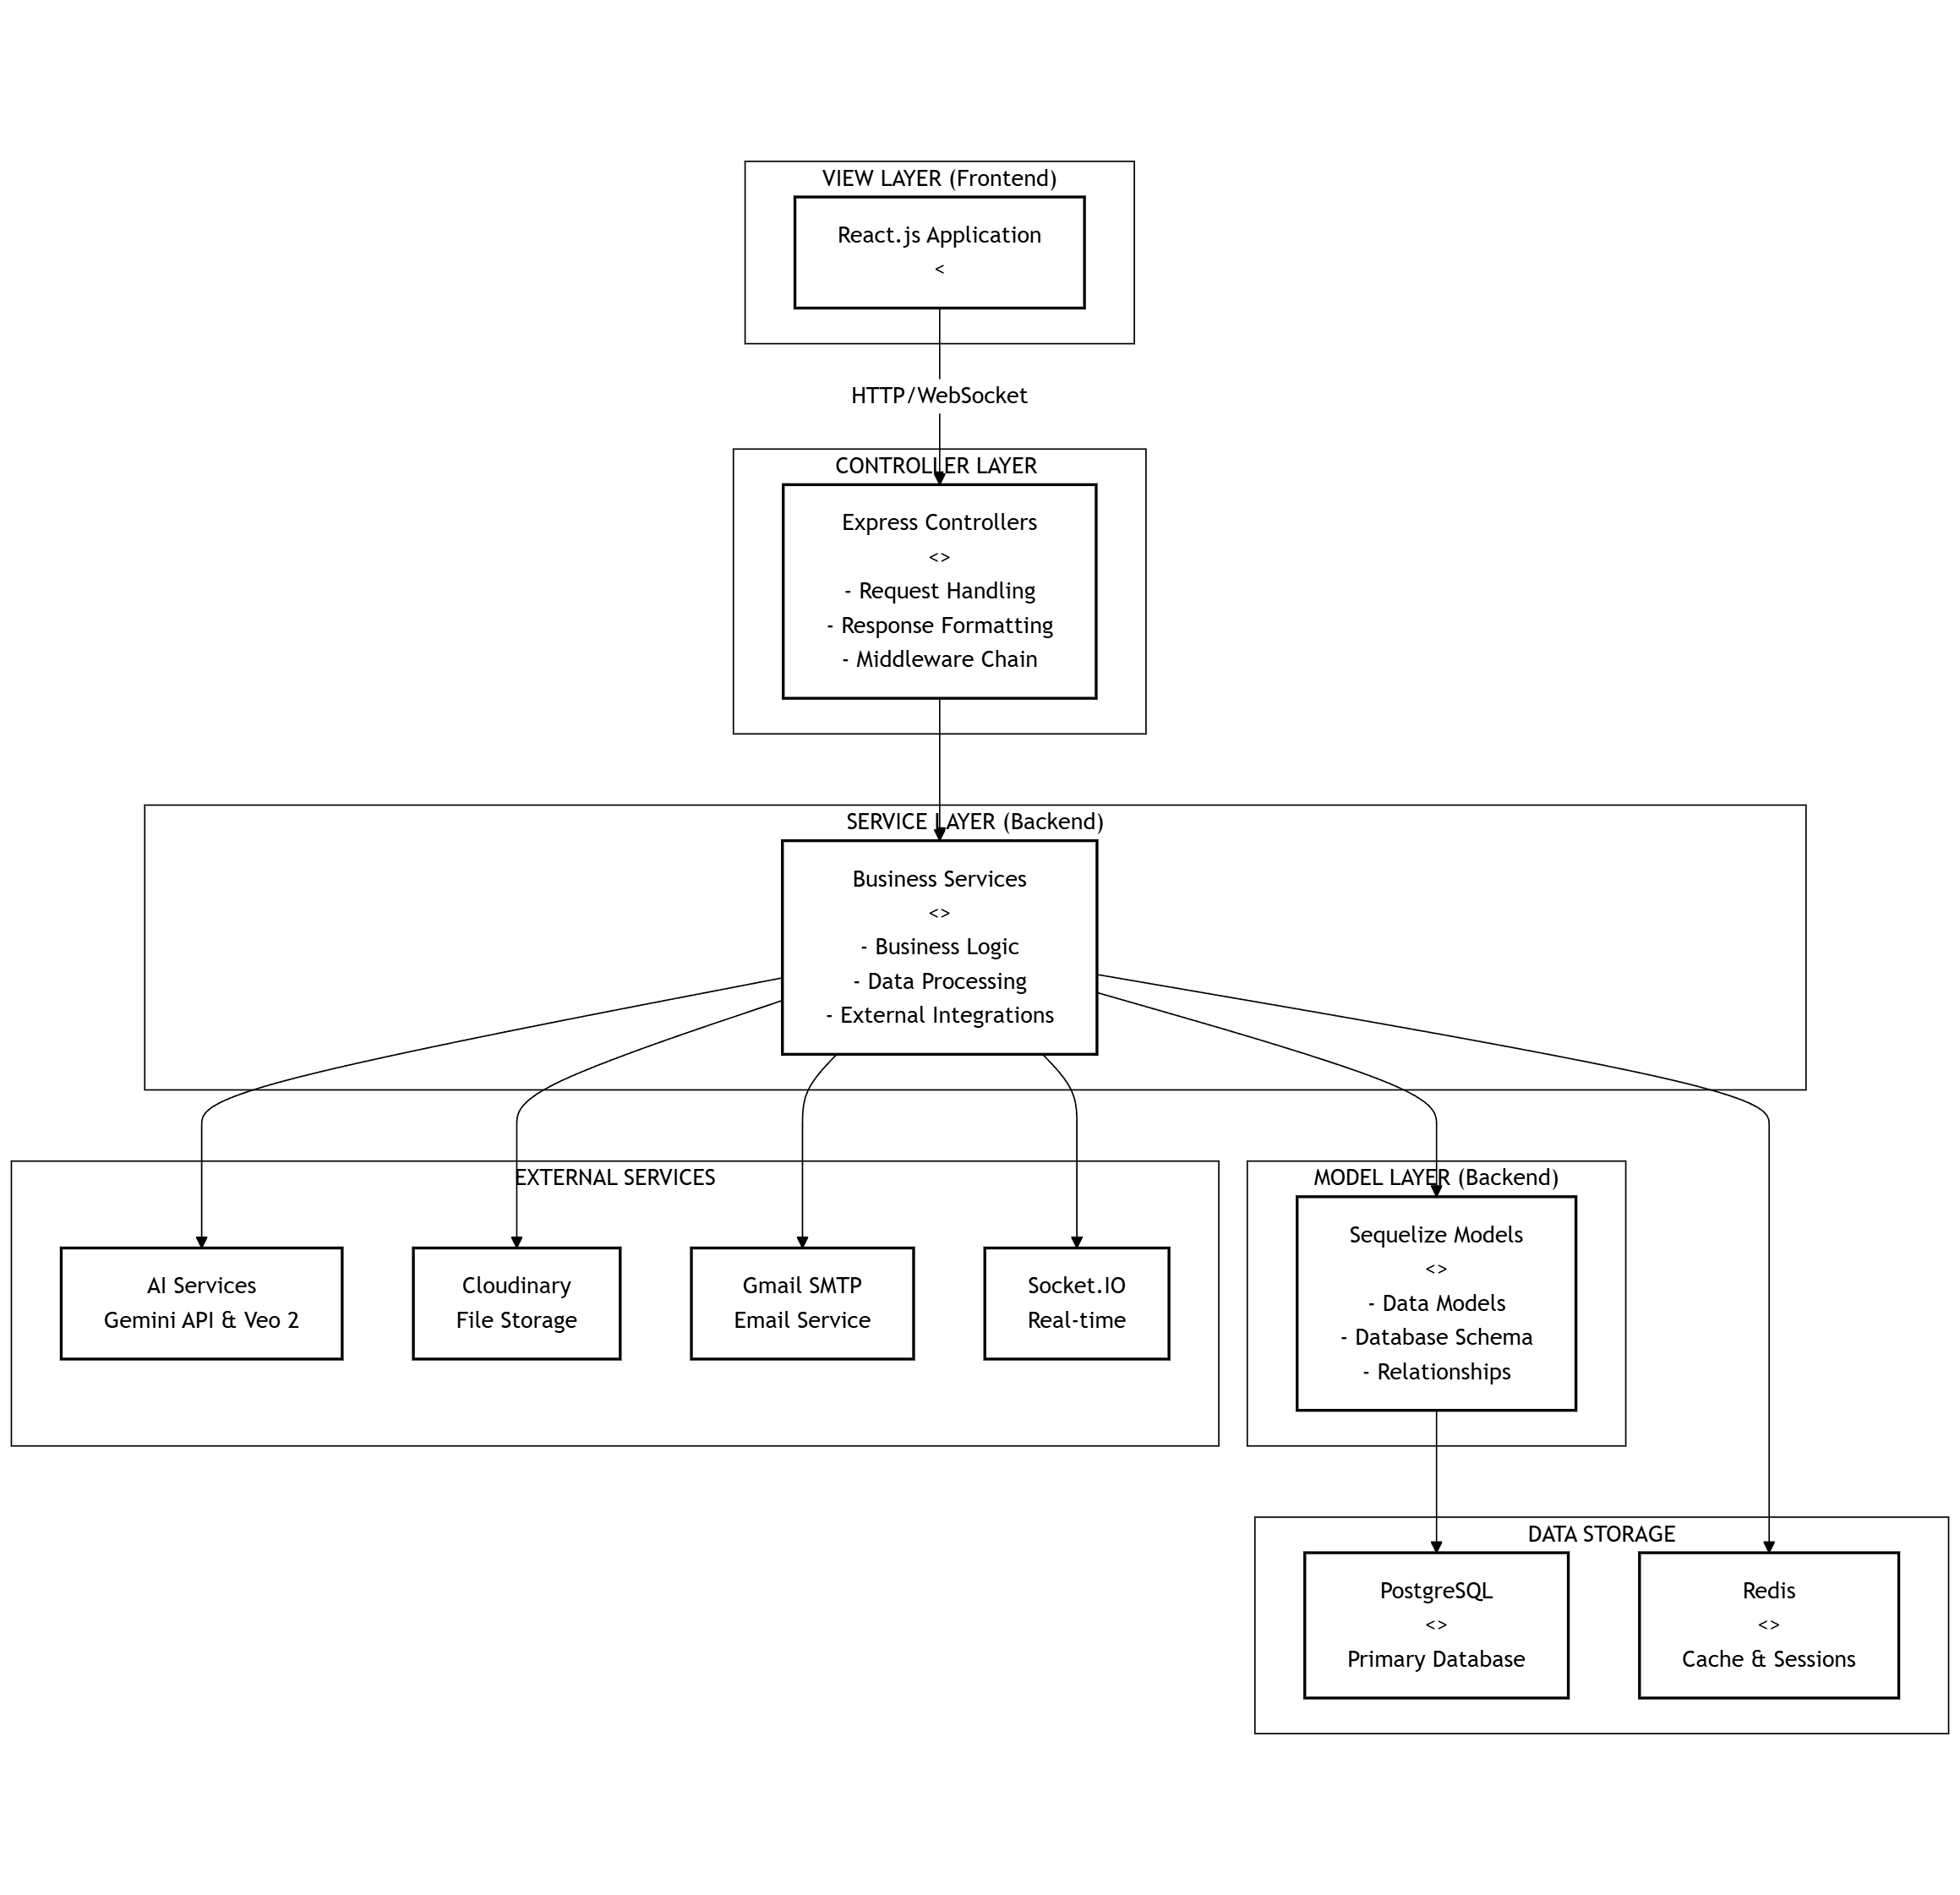
\includegraphics[width=0.9\textwidth]{Images/Component Diagrams/Component Diagram Overview.png}
    \caption{Component Diagram - Tổng quan hệ thống theo MVCS}
    \label{fig:component-overview}
\end{figure}

\paragraph{View Layer (Frontend)} \textbf{View Layer} được xây dựng bằng \textbf{React.js}, \textbf{TypeScript} và \textbf{Vite}, bao gồm:
\begin{itemize}
    \item \textbf{Main Frontend}: Ứng dụng cho buyer/seller/guest, gồm feed, marketplace, cart, checkout, orders, profile, groups, messages, notifications, AI creative lab, AI shopping assistant và seller dashboard.
    \item \textbf{Admin Frontend}: Ứng dụng riêng cho admin, gồm dashboard, users, content, reports, categories, sellers và settings.
    \item \textbf{State \& Context}: Quản lý auth state, notification state, messaging state và các state theo feature.
    \item \textbf{API Services}: Giao tiếp với backend qua REST API bằng fetch wrapper và kết nối Socket.IO cho real-time.
\end{itemize}

\paragraph{Controller Layer (Backend)} \textbf{Controller Layer} được xây dựng bằng \textbf{Express.js}, chịu trách nhiệm:
\begin{itemize}
    \item \textbf{Request Handling}: Nhận và xử lý HTTP request từ frontend.
    \item \textbf{Response Formatting}: Trả response thống nhất cho client.
    \item \textbf{Middleware Chain}: Áp dụng authentication, authorization, validation, rate limiting và error handling.
\end{itemize}

\paragraph{Service Layer (Backend)} \textbf{Service Layer} chứa business logic của hệ thống:
\begin{itemize}
    \item \textbf{Auth \& User Service}: Đăng ký, verify email, login, 2FA, reset password, profile và privacy settings.
    \item \textbf{Social Services}: Feed, posts, likes, comments, follow, saved items, groups và reports.
    \item \textbf{Commerce Services}: Products, variants, cart, orders, refunds, reviews, seller stats và product recommendations.
    \item \textbf{Realtime Services}: Messaging, notification và Socket.IO event emission.
    \item \textbf{AI Services}: Tạo nội dung text, image+text, lưu lịch sử AI, liên kết nội dung với post/scheduled post và cung cấp AI Shopping Assistant qua chatbox.
    \item \textbf{Admin Services}: Quản lý users, content, categories, seller verification và reports.
    \item \textbf{Cache Helper}: Đọc/ghi Redis cho các endpoint đọc nhiều như product list/detail, post list/detail, post comments và search; đồng thời xóa cache liên quan khi dữ liệu bài viết hoặc sản phẩm thay đổi.
\end{itemize}

\paragraph{Model/Data Access Layer (Backend)} \textbf{Model Layer} sử dụng \textbf{Prisma ORM} để:
\begin{itemize}
    \item \textbf{Data Models}: Định nghĩa schema dữ liệu tại \texttt{database/prisma/schema.prisma}.
    \item \textbf{Database Access}: Truy vấn và cập nhật PostgreSQL thông qua Prisma Client.
    \item \textbf{Relationships}: Quản lý quan hệ giữa users, products, orders, posts, groups, messages, notifications, reports và các bảng hỗ trợ.
\end{itemize}

\paragraph{Data Storage \& External Services} Hệ thống sử dụng:
\begin{itemize}
    \item \textbf{PostgreSQL}: Database chính lưu trữ dữ liệu nghiệp vụ.
    \item \textbf{Prisma Client}: Tầng ORM/data access cho backend.
    \item \textbf{Redis}: Cache tùy chọn cho dữ liệu đọc nhiều, được cấu hình bằng \texttt{REDIS\_URL}.
    \item \textbf{Cloudinary}: Lưu trữ và quản lý hình ảnh/file upload.
    \item \textbf{SMTP/Nodemailer}: Gửi email xác thực, OTP và reset password.
    \item \textbf{Socket.IO}: Giao tiếp real-time giữa frontend và core backend.
    \item \textbf{AI Providers}: Gemini cho text/vision; Hugging Face hoặc Replicate cho image generation nếu được cấu hình.
\end{itemize}

\paragraph{MVCS Flow} Luồng xử lý trong hệ thống:
\begin{enumerate}
    \item \textbf{View Layer} gửi request đến backend qua HTTP hoặc kết nối realtime qua Socket.IO.
    \item \textbf{Controller Layer} xác thực, validate và gọi service phù hợp.
    \item \textbf{Service Layer} thực hiện business logic và tương tác với Prisma Client.
    \item \textbf{Prisma Client} truy vấn hoặc cập nhật \textbf{PostgreSQL}.
    \item Với các endpoint đọc nhiều, \textbf{Controller/Cache Helper} có thể lấy dữ liệu từ \textbf{Redis} trước khi gọi service; khi có thay đổi dữ liệu, cache liên quan được invalidation theo pattern.
    \item \textbf{Service Layer} có thể gọi \textbf{Cloudinary}, \textbf{SMTP} hoặc \textbf{AI Providers} khi cần.
    \item Kết quả được trả về frontend; các sự kiện realtime được emit qua Socket.IO.
\end{enumerate}

\subsubsection{Component diagram theo vai trò người dùng}

Để dễ hiểu và phát triển các tính năng cụ thể, chúng tôi chia component diagram thành các diagram theo từng vai trò người dùng trong hệ thống.

\paragraph{Component diagram cho User/Buyer} \ref{fig:component-user-buyer} mô tả các components và flow dành cho người dùng thông thường (User/Buyer).

\begin{figure}[htbp]
    \centering
    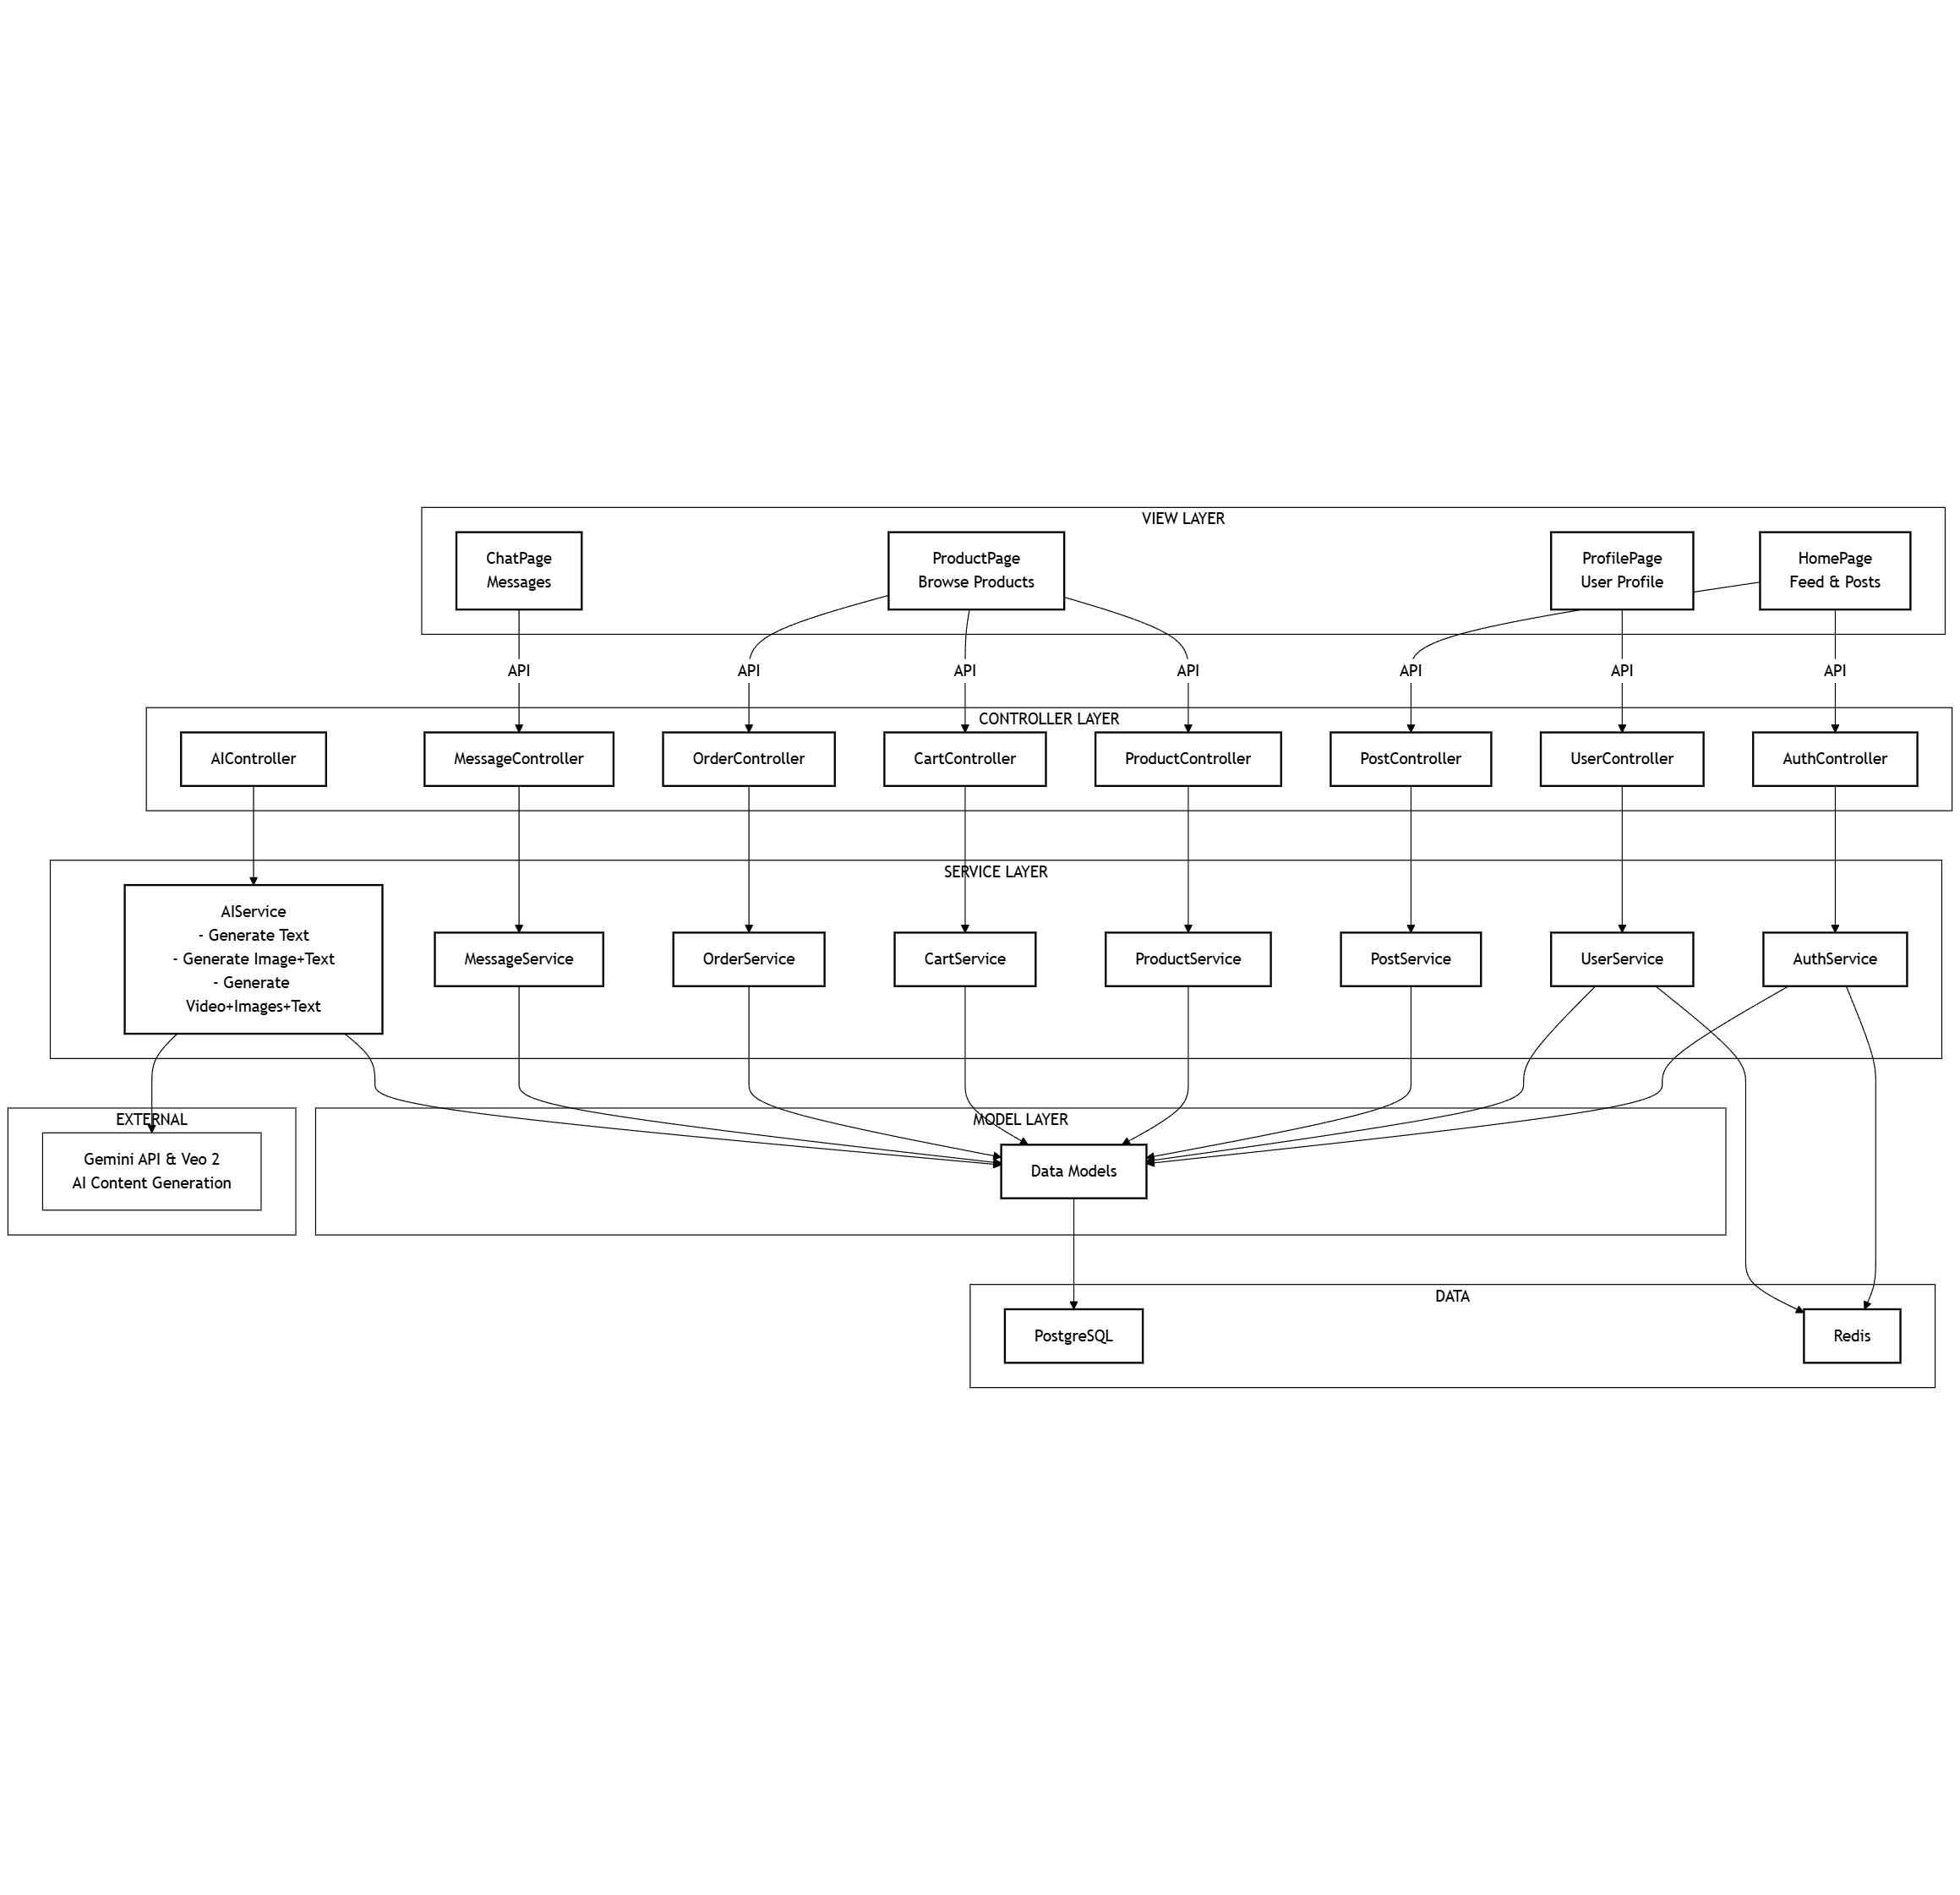
\includegraphics[width=0.9\textwidth]{Images/Component Diagrams/UserBuyer Component Diagram.png}
    \caption{Component Diagram - User/Buyer Role}
    \label{fig:component-user-buyer}
\end{figure}

\textbf{View Layer} bao gồm các trang:
\begin{itemize}
    \item \textbf{Feed/Home}: Trang feed, bài viết và tương tác xã hội.
    \item \textbf{Marketplace/Product Detail}: Duyệt, tìm kiếm, lọc và xem sản phẩm.
    \item \textbf{Cart/Checkout/Orders}: Giỏ hàng, đặt hàng, xác nhận thanh toán và theo dõi đơn.
    \item \textbf{Profile/Saved Items}: Hồ sơ, follow và danh sách đã lưu.
    \item \textbf{Groups/Messages/Notifications}: Nhóm cộng đồng, nhắn tin và thông báo.
\end{itemize}

\textbf{Controller Layer} xử lý các request từ frontend:
\begin{itemize}
    \item \textbf{AuthController, UserController}: Xác thực, profile, follow.
    \item \textbf{PostController, GroupController, ReportController}: Bài viết, nhóm, tương tác và báo cáo.
    \item \textbf{ProductController, CartController, OrderController, ReviewController}: Marketplace, giỏ hàng, đơn hàng và đánh giá.
    \item \textbf{MessageController, NotificationController}: Tin nhắn và thông báo realtime.
\end{itemize}

\textbf{Service Layer} thực hiện business logic tương ứng, còn \textbf{Model Layer} truy cập dữ liệu qua Prisma và PostgreSQL.

\paragraph{Component diagram cho Seller} \ref{fig:component-seller} mô tả các components và flow dành cho người bán (Seller).

\begin{figure}[htbp]
    \centering
    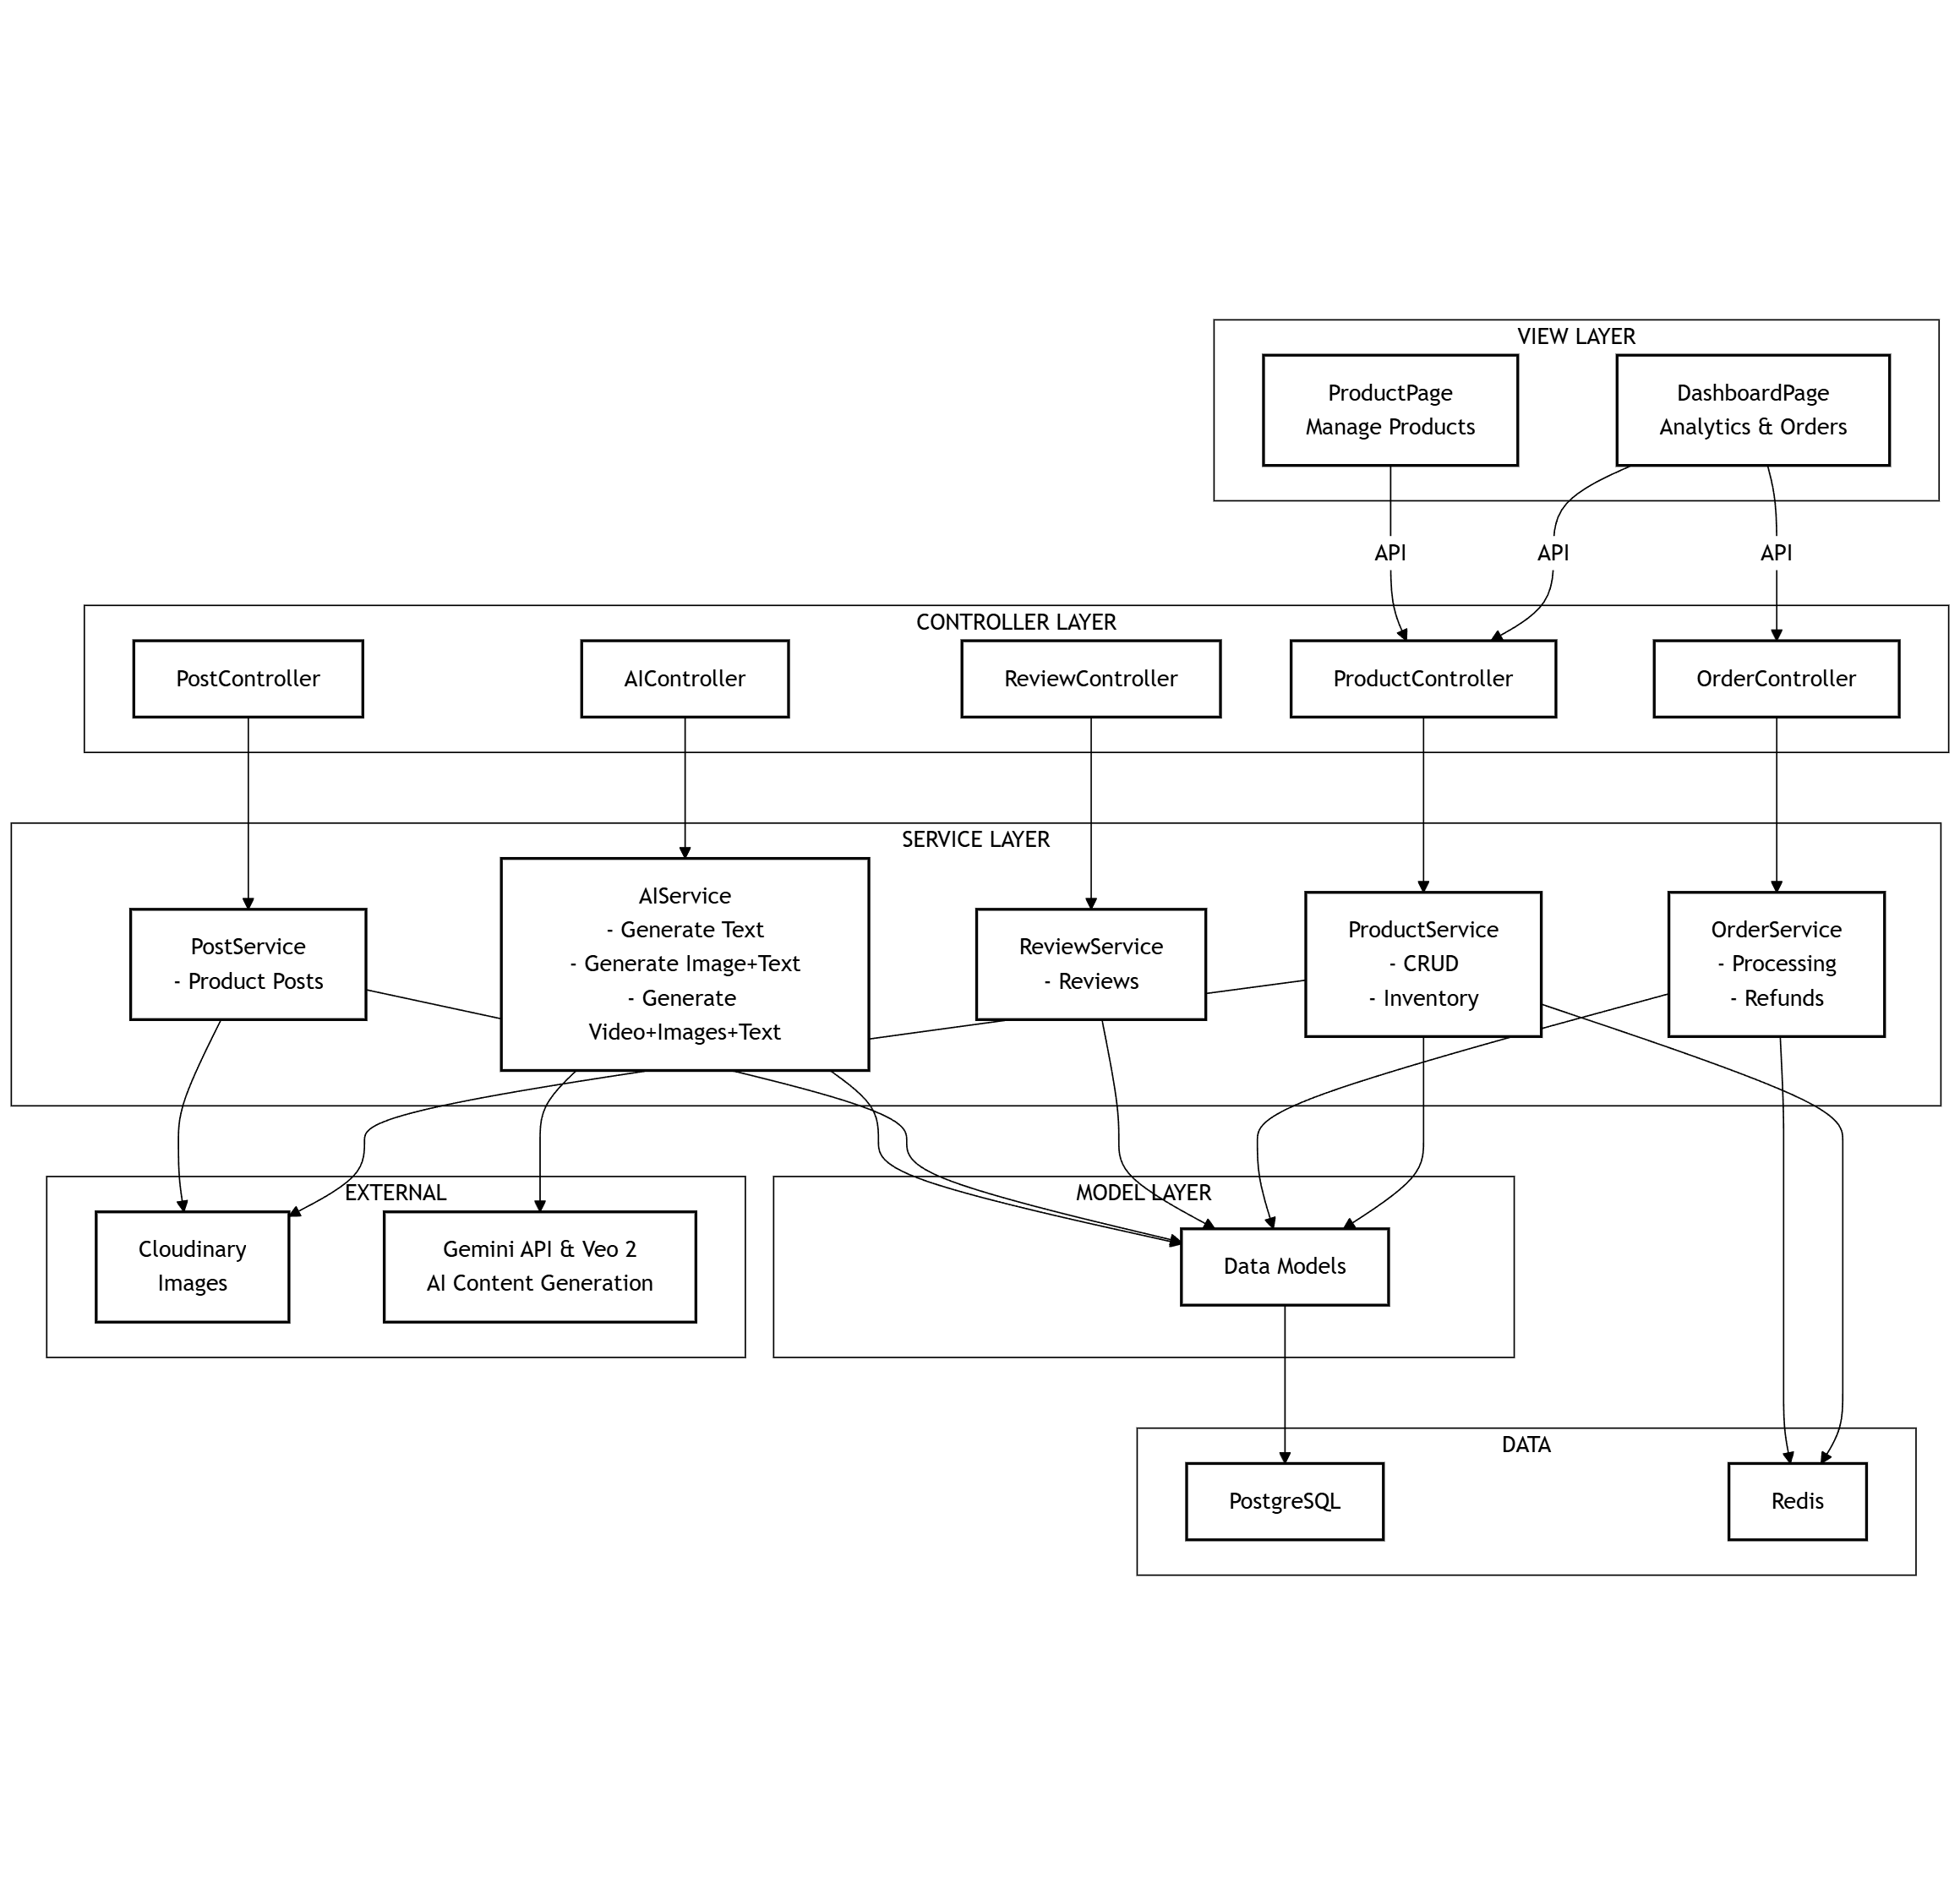
\includegraphics[width=0.9\textwidth]{Images/Component Diagrams/Seller Component Diagram.png}
    \caption{Component Diagram - Seller Role}
    \label{fig:component-seller}
\end{figure}

\textbf{View Layer} cho Seller bao gồm:
\begin{itemize}
    \item \textbf{Seller Registration}: Quy trình đăng ký seller nhiều bước, upload giấy tờ và theo dõi trạng thái duyệt.
    \item \textbf{Seller Dashboard}: Tổng quan doanh thu, đơn hàng, lượt xem và tồn kho.
    \item \textbf{Products/Inventory}: Quản lý sản phẩm, ảnh, biến thể, trạng thái và soft delete/restore.
    \item \textbf{Orders/Refunds/Reviews}: Quản lý đơn bán, xử lý hoàn tiền và phản hồi đánh giá.
    \item \textbf{Scheduled Posts/AI Lab}: Lên lịch bài đăng, tạo nội dung bằng AI và tư vấn mua sắm qua AI chatbox.
\end{itemize}

\textbf{Controller Layer} xử lý các chức năng của Seller:
\begin{itemize}
    \item \textbf{SellerController}: Đăng ký seller, xác minh hồ sơ, sensitive re-auth và change request.
    \item \textbf{ProductController}: Quản lý sản phẩm, inventory và variants.
    \item \textbf{OrderController}: Xem/cập nhật trạng thái đơn hàng và xử lý hoàn tiền.
    \item \textbf{ReviewController}: Phản hồi đánh giá.
    \item \textbf{ScheduledPostController}: CRUD bài đăng đã lên lịch và publish ngay.
    \item \textbf{AIController/AiAssistantController}: Tạo nội dung AI, quản lý lịch sử và xử lý chatbox tư vấn mua sắm.
\end{itemize}

Seller sử dụng \textbf{Cloudinary} để upload ảnh sản phẩm, shop logo/cover và giấy tờ xác minh.

\paragraph{Component diagram cho Admin} \ref{fig:component-admin} mô tả các components và flow dành cho quản trị viên (Admin).

\begin{figure}[htbp]
    \centering
    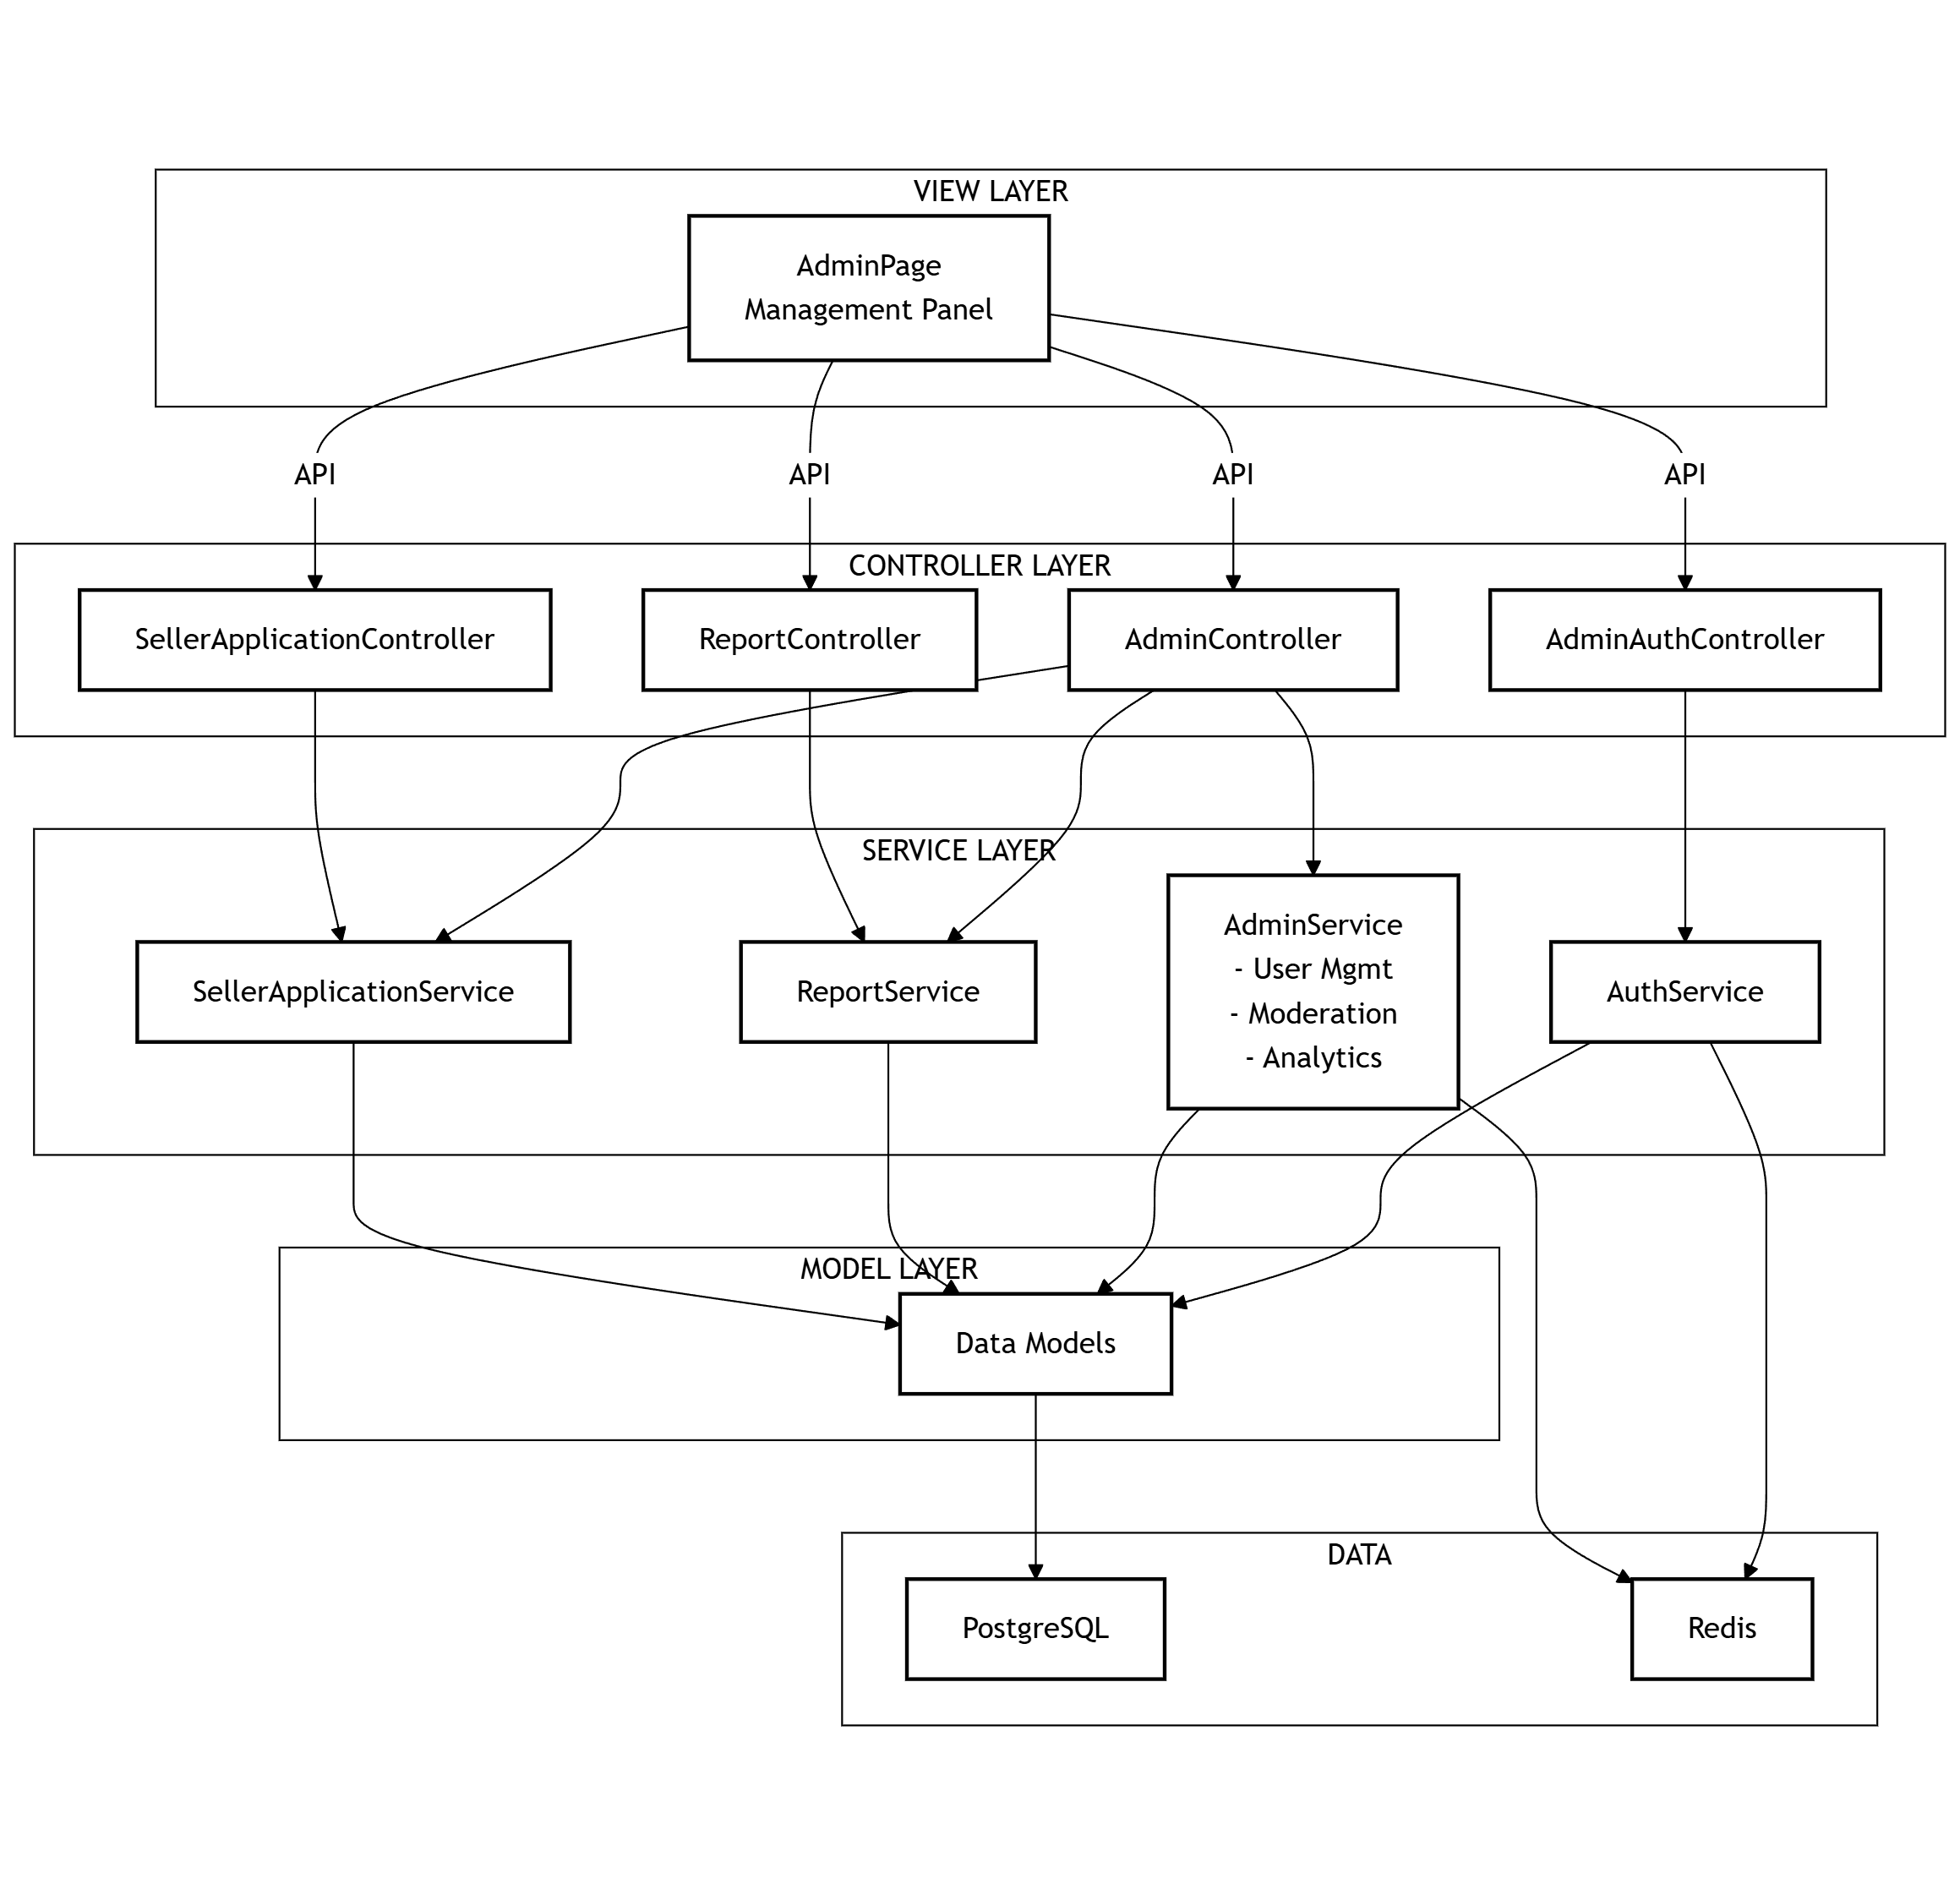
\includegraphics[width=0.9\textwidth]{Images/Component Diagrams/Admin Component Diagram.png}
    \caption{Component Diagram - Admin Role}
    \label{fig:component-admin}
\end{figure}

\textbf{View Layer} cho Admin bao gồm:
\begin{itemize}
    \item \textbf{Admin Login}: Đăng nhập admin qua admin API.
    \item \textbf{Dashboard}: Thống kê tổng quan và growth.
    \item \textbf{Users}: Quản lý user, trạng thái active và role.
    \item \textbf{Content}: Quản lý bài viết và sản phẩm.
    \item \textbf{Reports}: Xem và xử lý báo cáo vi phạm.
    \item \textbf{Categories}: Quản lý danh mục.
    \item \textbf{Sellers}: Duyệt hồ sơ seller và yêu cầu thay đổi dữ liệu nhạy cảm.
\end{itemize}

\textbf{Controller/Service Layer} cho Admin bao gồm:
\begin{itemize}
    \item \textbf{AdminAuthController/AuthService}: Xác thực admin.
    \item \textbf{AdminController/AdminService}: Users, content, categories và dashboard.
    \item \textbf{ReportController/ReportService}: Reports và moderation actions.
    \item \textbf{SellerAdmin Routes/SellerController}: Seller applications và sensitive change requests.
\end{itemize}

\paragraph{Lợi ích của việc chia nhỏ component diagram} Việc chia component diagram thành tổng quan và theo từng vai trò mang lại các lợi ích:
\begin{itemize}
    \item \textbf{Dễ hiểu}: Mỗi diagram tập trung vào một mục đích cụ thể.
    \item \textbf{Dễ maintain}: Cập nhật dễ hơn khi một module thay đổi.
    \item \textbf{Dễ phát triển}: Developers có thể tập trung vào diagram liên quan đến feature đang làm.
    \item \textbf{Dễ tài liệu hóa}: Tài liệu rõ ràng hơn cho từng user type và nhóm chức năng.
\end{itemize}


\section{Deployment Diagram}
Deployment diagram mô tả kiến trúc triển khai (deployment architecture) của hệ thống Social Commerce, bao gồm các thành phần phần cứng, phần mềm, môi trường triển khai và các kết nối giữa chúng. Diagram này giúp hiểu rõ cách hệ thống được triển khai trên môi trường production và cách các thành phần tương tác với nhau.

\subsection{Tổng quan kiến trúc triển khai}

\ref{fig:deployment-diagram} mô tả kiến trúc triển khai tổng thể của hệ thống, bao gồm các layers chính: Client Layer, CDN Layer, Application Server, Database và External Services.

\begin{figure}[htbp]
    \centering
    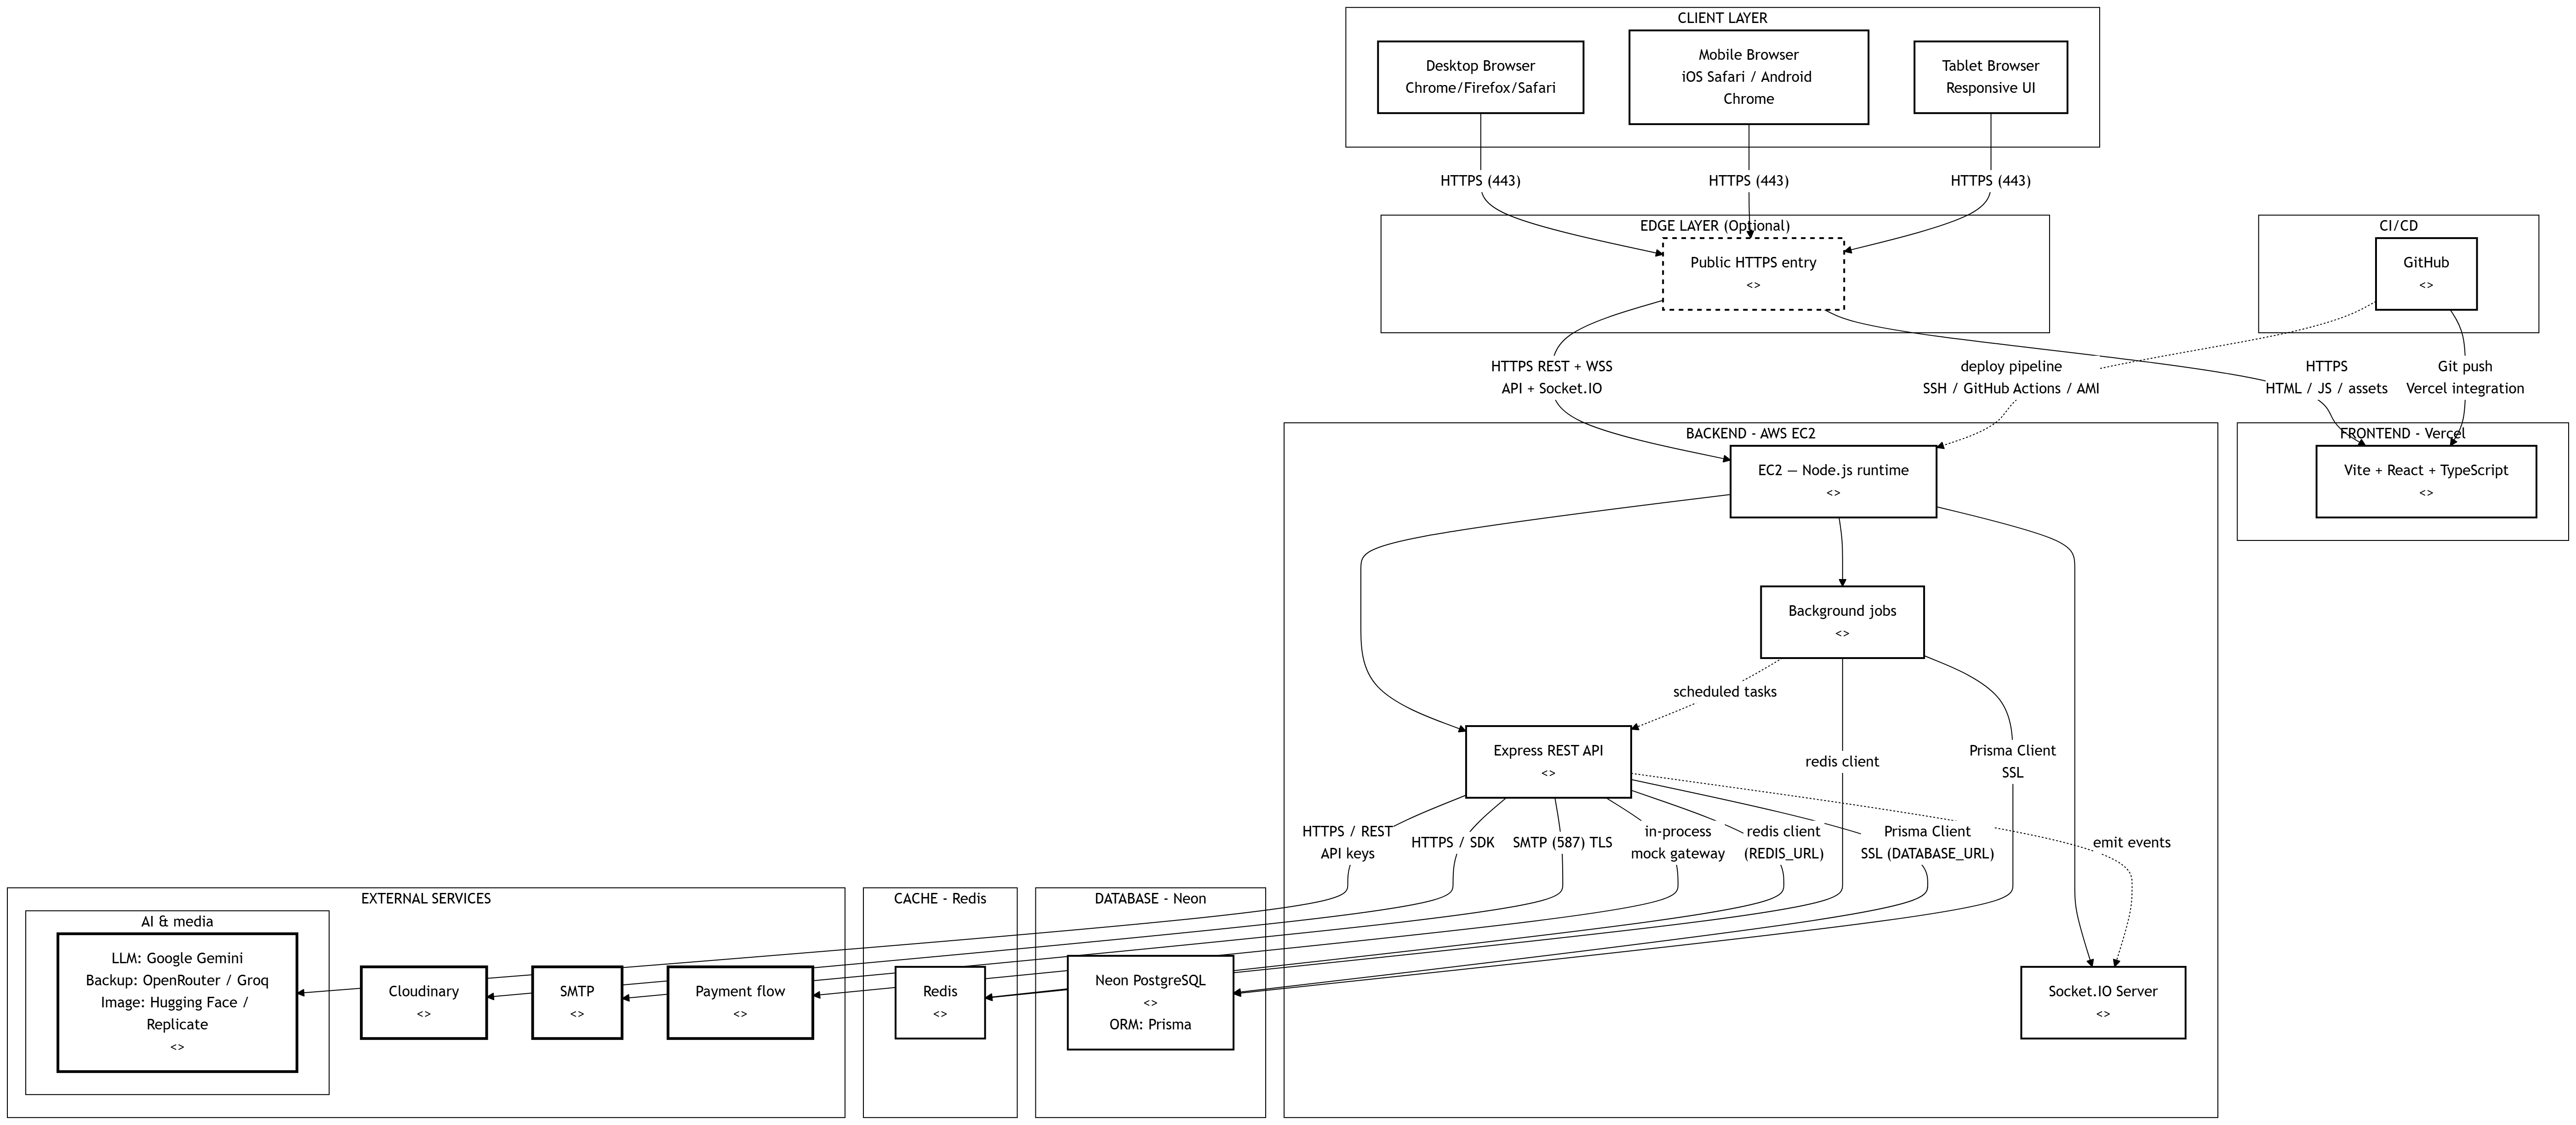
\includegraphics[width=\textwidth]{Images/Deployment Diagram.png}
    \caption{Deployment Diagram - Kiến trúc triển khai hệ thống}
    \label{fig:deployment-diagram}
\end{figure}

\subsection{Các thành phần chính}

\subsubsection{Client Layer}

\textbf{Client Layer} bao gồm các thiết bị và trình duyệt mà người dùng sử dụng để truy cập hệ thống:

\begin{itemize}
    \item \textbf{Desktop Browser}: Chrome, Firefox, Safari trên máy tính
    \item \textbf{Mobile Browser}: iOS Safari, Android Chrome trên điện thoại di động
    \item \textbf{Tablet Browser}: Giao diện responsive trên máy tính bảng
\end{itemize}

Tất cả các client kết nối đến hệ thống thông qua giao thức \textbf{HTTPS (port 443)} cho các request thông thường và \textbf{WebSocket Secure (WSS)} cho các tính năng real-time như thông báo và chat.

\subsubsection{CDN Layer (Optional)}

\textbf{Cloudflare CDN} là tầng tùy chọn được sử dụng để:

\begin{itemize}
    \item \textbf{Caching}: Lưu cache các static assets (HTML, CSS, JavaScript, images) để tăng tốc độ tải trang
    \item \textbf{DDoS Protection}: Bảo vệ hệ thống khỏi các cuộc tấn công DDoS
    \item \textbf{SSL/TLS Termination}: Xử lý chứng chỉ SSL/TLS, giảm tải cho application server
\end{itemize}

Khi CDN được triển khai, các static files sẽ được phục vụ từ CDN (cache hit), trong khi các request động sẽ được chuyển tiếp đến application server (cache miss). WebSocket connections có thể bypass CDN để kết nối trực tiếp với application server để đảm bảo độ trễ thấp.

\subsubsection{Application Server}

Hệ thống được triển khai trên \textbf{Render.com}, một platform-as-a-service (PaaS) cloud, với các thành phần sau:

\paragraph{Node.js Runtime} 
Môi trường thực thi sử dụng \textbf{Node.js version >= 18.0.0}, cung cấp nền tảng để chạy ứng dụng backend.

\paragraph{React Frontend}
Frontend được build bằng \textbf{Vite} và được deploy dưới dạng static files. Trong production, Express server phục vụ các static files này từ thư mục \texttt{frontend/dist/}, bao gồm:
\begin{itemize}
    \item HTML files
    \item JavaScript bundles
    \item CSS stylesheets
    \item Assets (images, fonts, etc.)
\end{itemize}

\paragraph{Express API Server}
Backend được xây dựng bằng \textbf{Express.js framework}, chịu trách nhiệm:
\begin{itemize}
    \item Xử lý các REST API endpoints
    \item Áp dụng middleware stack (authentication, validation, rate limiting, error handling)
    \item Thực thi business logic thông qua controllers
    \item Tích hợp với các external services
\end{itemize}

\paragraph{Socket.IO Server}
\textbf{Socket.IO server} được tích hợp vào cùng application server, cung cấp:
\begin{itemize}
    \item \textbf{WebSocket connections}: Kết nối real-time hai chiều với clients
    \item \textbf{Real-time events}: Gửi và nhận events real-time
    \item \textbf{Chat rooms}: Quản lý các phòng chat
    \item \textbf{Push Notifications}: Gửi thông báo tức thì đến clients
    \item \textbf{Live Updates}: Cập nhật trạng thái real-time (order status, notifications, etc.)
\end{itemize}

Socket.IO server tương tác với Express server để emit events khi có các thay đổi trong hệ thống (ví dụ: khi có đơn hàng mới, notification mới).

\paragraph{Background Jobs}
Hệ thống sử dụng \textbf{node-cron} để chạy các background jobs theo lịch:
\begin{itemize}
    \item \textbf{Auto-publish scheduled posts}: Tự động publish các bài viết đã được lên lịch
    \item \textbf{Cleanup old notifications}: Xóa các thông báo cũ
    \item \textbf{Reset monthly AI usage}: Reset số lần sử dụng AI theo tháng
    \item \textbf{Clean expired content requests}: Xóa các yêu cầu tạo nội dung AI đã hết hạn
\end{itemize}

Các cron jobs được chạy in-process trong cùng application server, không cần infrastructure riêng biệt.

\subsubsection{Database - PostgreSQL}

Hệ thống sử dụng \textbf{PostgreSQL} làm database chính:

\begin{itemize}
    \item \textbf{Managed Database}: Database được quản lý bởi Render.com hoặc cloud provider khác
    \item \textbf{ORM: Sequelize}: Sử dụng Sequelize ORM để tương tác với database, cung cấp abstraction layer và hỗ trợ migrations
    \item \textbf{SSL/TLS Connection}: Tất cả các kết nối đến database đều được mã hóa bằng SSL/TLS để đảm bảo bảo mật
\end{itemize}

Express server và cron jobs đều kết nối đến PostgreSQL thông qua Sequelize ORM để thực hiện các thao tác CRUD và query dữ liệu.

\subsubsection{External Services}

Hệ thống tích hợp với các external services để cung cấp các tính năng bổ sung:

\paragraph{AI Services}
\textbf{Google Gemini API và Google Veo 2} được sử dụng để:
\begin{itemize}
    \item Tạo bài viết từ mô tả, ý tưởng và hình ảnh sản phẩm (Generate Text)
    \item Tạo đồng thời bài viết và hình ảnh từ mô tả, ý tưởng và hình ảnh đầu vào (Generate Image + Text)
    \item Tạo video ngắn kèm tối đa 3 hình ảnh và bài viết từ mô tả, ý tưởng và hình ảnh đầu vào (Generate Video + Images + Text)
\end{itemize}

Kết nối đến Gemini API và Veo 2 sử dụng HTTPS/REST với API Key authentication. Hệ thống quản lý usage limit cho từng người dùng để kiểm soát chi phí và tài nguyên.

\paragraph{File Storage}
\textbf{Cloudinary} được sử dụng để:
\begin{itemize}
    \item Lưu trữ và quản lý hình ảnh, video
    \item Tối ưu hóa hình ảnh (resize, compress, format conversion)
    \item Cung cấp CDN global để phân phối assets nhanh chóng
\end{itemize}

Kết nối đến Cloudinary sử dụng HTTPS/REST API để upload và quản lý files.

\paragraph{Email Service}
\textbf{Gmail SMTP} được sử dụng để:
\begin{itemize}
    \item Gửi email thông báo đến người dùng
    \item Gửi email xác nhận đơn đăng ký seller
    \item Gửi email thông báo về đơn hàng, reviews, etc.
\end{itemize}

Kết nối sử dụng SMTP protocol (port 587) với TLS encryption, thông qua Nodemailer library.

\paragraph{Payment Simulator}
\textbf{Payment Simulator} là một mock service chạy local trong application server:
\begin{itemize}
    \item Mô phỏng quá trình thanh toán (success/failure)
    \item Chỉ sử dụng cho development và testing
    \item Không có kết nối mạng ngoài, không xử lý tiền thật
\end{itemize}

\subsubsection{CI/CD Pipeline}

\textbf{GitHub} được sử dụng làm repository để:
\begin{itemize}
    \item Lưu trữ source code
    \item Version control
    \item Quản lý pull requests và code reviews
\end{itemize}

\subsection{Đặc điểm kiến trúc}

\paragraph{Monolithic Deployment}
Hệ thống được triển khai dưới dạng monolithic architecture, tất cả các components (Frontend, Backend API, Socket.IO, Cron Jobs) chạy trong cùng một application server. Điều này đơn giản hóa việc triển khai và quản lý, phù hợp với quy mô hiện tại của dự án.

\paragraph{Server-Side Rendering Static Files}
Frontend React được build thành static files và được phục vụ bởi Express server. Điều này cho phép:
\begin{itemize}
    \item Single deployment cho cả frontend và backend
    \item Không cần CDN riêng cho static files (tùy chọn)
    \item Dễ dàng quản lý và deploy
\end{itemize}

\paragraph{Real-time Communication}
Socket.IO được tích hợp trực tiếp vào application server, cho phép real-time communication mà không cần infrastructure riêng biệt. Điều này đơn giản hóa kiến trúc nhưng có thể ảnh hưởng đến khả năng mở rộng (scalability) nếu số lượng WebSocket connections tăng cao.

\paragraph{External Service Integration}
Hệ thống tích hợp với các external services thông qua REST API và SMTP, giúp:
\begin{itemize}
    \item Giảm tải cho application server (file storage, email sending)
    \item Tận dụng các dịch vụ chuyên nghiệp (AI content generation, cloud storage)
    \item Dễ dàng thay thế hoặc bổ sung services khi cần
\end{itemize}

\paragraph{Bảo mật}
Tất cả các kết nối đều được mã hóa:
\begin{itemize}
    \item Client $\leftrightarrow$ Server: HTTPS/WSS (SSL/TLS)
    \item Application $\leftrightarrow$ Database: SSL/TLS connection
    \item Application $\leftrightarrow$ External Services: HTTPS (REST API) hoặc TLS (SMTP)
\end{itemize}

